\documentclass[hidelinks]{thesis}
\setlength{\marginparwidth}{2.5cm}
\usepackage[utf8]{inputenc}
\usepackage[pdftex,
            pdfauthor={James Hales},
            pdftitle={Quantifying over epistemic updates}]{hyperref}
\usepackage{notation}
\usepackage{subcaption}
\usepackage{tikz}
\usetikzlibrary{arrows}
\usetikzlibrary{fit}
\usetikzlibrary{positioning}

\title{Quantifying over epistemic updates}
\author{James Hales}
\date{May, 2016}

\keywords{
Refinement modal logic,
arbitrary action model logic,
dynamic epistemic logic,
epistemic protocol synthesis,
modal logic,
expressivity,
axiomatisations,
decision procedures.
}

\categories{
F.4.1 [Theory of Computation] Mathematical Logic and Formal Languages - Mathematical Logic, 
I.2.4 [Computing Methodolodies] Knowledge Representation Formalisms and Methods - Modal Logic.
}

\begin{document}
    
    \maketitle

    \begin{acknowledgements}
\todo[inline]{Acknowledgements}
\end{acknowledgements}

    \begin{abstract}
\todo[inline]{Abstract}
\end{abstract}


    \tableofcontents
    %\listoftables
    %\listoffigures

    \chapter{Introduction}\label{introduction}

Epistemic logic is the logic of knowledge, used to reason about the knowledge of a collection of agents hold regarding the truth of propositional atoms and each other's knowledge.
As a modal logic, situations involving knowledge are represented by relational structures known as Kripke models, and are reasoned about using modal operators that denote that an agent knows that a statement is true.
Epistemic logic only considers static situations involving knowledge, where knowledge and the truth of the propositional atoms that the knowledge is about do not change.
However many practical situations involving knowledge are not static, and many natural questions about knowledge directly concern changes in knowledge.
For example, your knowledge may change as a result of reading this dissertation, and you might ask ``What will I know after reading this dissertation?'', ``Will I know about epistemic updates after reading this dissertation?'' or ``How can I learn about epistemic updates?''.

Dynamic epistemic logics are logics of change of knowledge, used to reason about how knowledge changes in response to epistemic updates, events that provide agents with additional information.
Examples of epistemic updates include the direct observation of information by an agent, communication of information between agents, and epistemic protocols formed by composing simpler epistemic updates sequentially, concurrently, or conditionally.
For our purposes, when we discuss epistemic updates we assume that they are purely informative in nature, so they may cause knowledge to change, but not the truth of the propositional atoms that the knowledge is about.
We also assume that epistemic updates increase certainty about information monotonically, so they may not cause agents to forget or revise information that they were previously certain of. 

Previous work in dynamic epistemic logic has considered how knowledge changes in response to specific epistemic updates.
Notable works include the public announcement logic of Plaza~\cite{plaza:1989} and Gerbrandy and Groenveld~\cite{gerbrandy:1997}, and the action model logic of Baltag, Moss and Solecki~\cite{baltag:1998,baltag:2004}, which each introduce models for epistemic updates and logics for reasoning about the effects of specific epistemic updates using these models.
These logics extend epistemic logic with operators that denote that a specific epistemic update results in a statement becoming true, allowing us to answer questions such as ``Will I know about quantifying over epistemic updates after reading this dissertation?''.
Both logics represent changes in knowledge as operations that take a Kripke model representing a situation involving knowledge, and a model representing an epistemic update, and produces a new Kripke model, representing the result of the epistemic update.
These operations for performing epistemic updates on Kripke models give a powerful method for modelling and reasoning about the full effects of a specific epistemic update in a specific situation, allowing us to answer questions such as ``What will I know after reading this dissertation?''.
However many natural questions about changes in knowledge are not questions about specific epistemic updates, such as ``{\em How} can I learn about quantifying over epistemic updates?''.

More recent work in dynamic epistemic logic has considered the knowledge changes in response to arbitrary epistemic updates, by quantifying over epistemic updates.
Notable works include the arbitrary public announcement logic (\logicApal{}) of Balbiani, et al.~\cite{balbiani:2007} and the group announcement logic (GAL) of {\AA}gotnes, et al.~\cite{agotnes:2008,agotnes:2010}, which each introduce logics for quantifying over epistemic updates.
These logics extend public announcement logic with quantifiers that denote either that every epistemic update or some epistemic update results in a statement becoming true, allowing us to answer questions such as ``Can I learn about quantifying over epistemic updates (through some epistemic update)?''.
Supposing that the answer is in the affirmative we might subsequently ask ``How can I learn about quantifying over epistemic updates?'', expecting an example of a specific epistemic update that will result in the desired change in knowledge.
In principle, such questions may be answered by model-checking, decision and synthesis procedures for these logics.
However although both of these logics have model-checking procedures~\cite{agotnes:2010}, they are undecidable~\cite{agotnes:2014}.
In the present work we introduce several decidable logics for quantifying over epistemic updates, in the same style as \logicApal{} and GAL, but quantifying over different models for epistemic updates: refinement modal logic, arbitrary action model logic.

Refinement modal logic (\logicRml{}) is an extension of epistemic logic that introduces quantifiers over {\em refinements} of Kripke models.
Refinements correspond to the results of a very general notion of epistemic updates, in accordance with our informal understanding of epistemic updates as purely informative and monotonically increasing certainty of information.
The refinements of a Kripke model partially correspond to the results of action models, but are more general.
Unlike public announcements or action models, refinements in general are not backed by a model or operation for epistemic updates that produces the results.
We consider \logicRml{} in a variety of modal settings, including \classK{}, \classKF{}, \classKFF{}, \classKD{} and \classS{}.
In the settings of \classK{}, \classKFF{}, \classKD{} and \classS{} we provide sound and complete axiomatisations for \logicRml{}, we show that \logicRml{} is decidable and that \logicRml{} is expressively equivalent to modal logic.
In the setting of \classKF{} we show that \logicRml{} is decidable, and that its expressivity lies strictly between that of modal logic and the modal $\mu$-calculus.

Arbitrary action model logic (\logicAaml{}) is an extension of action model logic that introduces quantifiers over action models.
Like \logicRml{}, we consider \logicAaml{} in a variety of settings, including \classK{}, \classKFF{} and \classS{}.
In these settings we provide sound and complete axiomatisations, we show that \logicAaml{} is decidable and that \logicAaml{} is expressively equivalent to modal logic.
Moreover we show that action model quantification is equivalent to refinement quantification and we provide a synthesis procedure that constructs a specific action model that results in a desired change in knowledge whenever such an action model exists.

In Chapter~\ref{literature} we provide an overview of literature in epistemic logic and dynamic epistemic logic, giving context and motivation to the present work.
In Chapter~\ref{technical} we recall technical definitions and results used in the following chapters.
In Chapter~\ref{rml} we introduce the refinement modal logic in various settings, providing semantic results about refinements, sound and complete axiomatisations, and expressivity and decidability results.
In Chapter~\ref{aaml} we introduce the arbitrary action model logic in various settings, providing sound and complete axiomatisations, expressivity and decidability results, methods for action model synthesis, and we show that action model quantifiers are equivalent to refinement quantifiers.
Finally in Chapter~\ref{conclusion} we summarise our results, and outline on-going work and open questions.

    \chapter{Literature review}\label{literature}

Dynamic epistemic logics are logics of change of knowledge used to reason about how knowledge changes in response to epistemic updates.
Often the effects of epistemic updates on knowledge can be unintuitive or surprising: sometimes announcing a true statement makes it become false, as in Fitch's knowability paradox~\cite{fitch:1963}; sometimes repeating a statement can provide different information each time it is repeated, as in the muddy children puzzle~\cite{barwise:1981, vanditmarsch:2007}. 
Being able to reason about changes of knowledge has applications in a range of areas:
in artificial intelligence and information science we want to represent and reason about updates in knowledge bases and ontologies;
in the study of network protocols and computer security we want to ensure that information communicated through a network results in the desired knowledge-based goals
 and that information that is communicated doesn't result in the leaking of sensitive information; and
in economics and game theory we want to reason about processes or games with imperfect knowledge, where actions may provide players with additional information that's required to inform their decisions.
For some applications it's useful to know the effects of specific epistemic updates~\cite{plaza:1989,baltag:1998}, such as when a robot updates its internal knowledge base with with new sensor information, when a participant in a network protocol sends or receives a message containing new information, or a player in a game performs an action that reveals additional information about the game state.
At other times it's useful to reason about arbitrary epistemic updates in a goal-directed fashion~\cite{balbiani:2007,agotnes:2010,vanditmarsch:2009}, such as when a robot must sense enough of its environment to navigate an area, when a protocol designer must design a protocol that achieves desired knowledge-based goals whilst remaining secure, or when a player in a game must choose a strategy that maximises the information available in order to better inform their decisions.
Formal logics of knowledge have existed for many decades~\cite{vonwright:1951,hintikka:1957,hintikka:1961,hintikka:1962}, whilst logics for reasoning about the effects of specific epistemic updates have only arisen relatively recently~\cite{plaza:1989,gerbrandy:1997,baltag:1998}. 
Much more recently logics for reasoning about arbitrary epistemic updates have been considered~\cite{balbiani:2007,vanditmarsch:2009,agotnes:2010}, and logics of this variety are the focus of our research.
This review summarises the development of logics of knowledge, logics of specific epistemic updates and finally logics of arbitrary epistemic updates.  

\section{Logics of knowledge}

Epistemic logic is the modal logic of knowledge.
Modal logics extend propositional logic with modal operators that qualify the truth of statements in the logic.
In epistemic logic, the modal operators allow us to qualify the truth of a statement by saying that an agent knows that the statement is true.
For example, we can qualify the proposition ``The coin has landed heads up'' by saying ``Alice knows that the coin has landed heads up''.
Modal operators may also be nested, allowing us to make statements about an agent's knowledge about its own or another agent's knowledge.
For example, we could say ``Alice knows that Alice knows that the coin has landed heads up'', or ``Bob doesn't know that Alice knows that the coin has landed heads up''.

The semantics for many modal logics, including epistemic logic, are based in relational structures known as Kripke models~\cite{kripke:1963,blackburn:2001}.
A Kripke model is a labelled graph over a set of worlds, where each world has a set of propositional atoms that are true at that world, and each agent has an accessibility relation defined over the worlds.
At a particular world, an agent considers another world to be ``possible'' if that world is accessible from the given world through the agent's accessibility relation in the Kripke model.
An agent is said to ``know'' that a statement is true in a given world if that statement is true on each of the worlds that the agent considers possible.

Variants of modal logic may attribute different intuitive meanings to its modal operators, often depending on properties required of the Kripke models that are under consideration.
For example epistemic logics usually require that agents always consider the current, real, world to be possible, as otherwise the agent might ``know'' a statement that is actually false in the real world.
By contrast, doxastic logics, which are logics of belief, often relax this constraint as it's reasonable for an agent to ``believe'' a statement that is actually false in the real world.

\subsection{Modal and epistemic logics}

Lewis and Langford are widely acknowledged as the progenitors of early modal logic, with the earliest symbolic treatment of modal logic dating back to work by Lewis in 1912, and leading to a book with Langford~\cite{langford:1959} in 1959.
Early work in modal logic was mostly syntactic, lacking any formal semantics.
Carnap~\cite{carnap:1946, carnap:1947} first considered the notion of possible worlds to represent the semantics of modal logics, and other authors, amongst them Hintikka~\cite{hintikka:1957, hintikka:1961} and Kripke~\cite{kripke:1959} further developed these semantics, resulting in the final form by Kripke~\cite{kripke:1963}, the namesake of Kripke models and Kripke semantics for modal logics.
von Wright~\cite{vonwright:1951} was responsible for the first logical analysis of knowledge in terms of modal logic in 1951, and this was further developed by Hintikka~\cite{hintikka:1957,hintikka:1961} culminating in the first book-length treatment of the subject by Hintikka~\cite{hintikka:1962} in 1962.

\subsection{Common knowledge}

The first work on the topic of common knowledge was by Lewis~\cite{lewis:1969} and later work was by McCarthy, Sato, Hayashi and Igarishi~\cite{mccarthy:1979}.
Common knowledge is described by McCarthy as what ``any fool knows''; for a statement to be common knowledge, it is required that everyone knows that the statement is true, that every agent knows that every agent knows that the statement is true, and so on.
Whereas the definition of common knowledge of Lewis and McCarthy was in terms of modal logics, Aumann~\cite{aumann:1976} gave an alternative definition for common knowledge using Aumann structures and the meet of structures rather than Kripke models and modal formulas.
Common knowledge is of interest in economics and game theory, where common knowledge of rationality, rules and outcomes is assumed in order to permit backwards-induction reasoning about games~\cite{aumann:1995}.
Aumann~\cite{aumann:1976} discusses common knowledge with a focus towards discussing economics and game theory. 
Lehmann~\cite{lehmann:1984} and Halpern and Moses~\cite{halpern:1985} considered common knowledge in depth, and the book by Fagin, Halpern, Moses and Vardi~\cite{fagin:1995} gives a survey of much of their work in this area.

\subsection{Alternative logics of knowledge}

Non-modal logics of knowledge have been considered. 
Aumann~\cite{aumann:1976} proposed an event-based approach using Aumann structures, which represents knowledge as an operator on events rather than reasoning about knowledge using logical formulas.
There is in fact a one-to-one correspondence between epistemic Kripke models and Aumann structures~\cite{fagin:1995}.
A number of authors, among them van Emde Boas, Groenendijk, and Stokhof~\cite{vanemdeboas:1980}, Fagin and Vardi~\cite{fagin:1985}, Mertens and Zamir~\cite{mertens:1985} and Fagin, Halpern and Vardi~\cite{fagin:1991} have considered modeling knowledge and belief using an infinite hierarchy of sets representing the relative strength or plausibility of each piece of knowledge.
This representation lends itself easily to the concept of belief revision, discussed in the next section.
Fagin, Halpern and Vardi~\cite{fagin:1991} discussed the relationship between this representation of knowledge and belief with modal logic.  

%\subsection{Applications of logics of knowledge}

%\begin{enumerate}
    %\item McCarthy 1979 - Knowledge and belief for machines~\cite{mccarthy:1979b}
    %\item Aumann [5~\cite{aumann:1976},6~\cite{aumann:1999},7~\cite{aumann:1995}] -
        %Economics and Game theory

    %\item Orlowska 1989 - Knowledge as operator on events~\cite{orlowska:1989}
    %\item Brandenburger, et al. 1993, etc. - "Direct" representation of
        %knowledge~\cite{brandenburger:1993}
    %\item Fagin, Halpern, Vardi 1991 - Relationship of Brandenburger knowledge
        %to ML~\cite{fagin:1991}
    %\item Levesque 1984a - KD45 as knowledge~\cite{levesque:1984a}
    %\item Fagin and Halpern 1988a, Levesque 1984b - KD45 as
        %belief~\cite{fagin:1987, levesque:1984b}
    %\item Friedman and Halpern 1977, Kraus and Lehmann 1988, Moses and Shoham
        %1933, Voorbraak 1992 - System with knowledge and belief, interaction
    %between knowledge and belief~\cite{friedman:1997, kraus:1988, moses:1993,
    %voorbraak:1992}
    %% TODO AI, economics, game theory
%\end{enumerate}

\section{Logics of specific epistemic updates}

Dynamic epistemic logics consider how knowledge changes as a result of epistemic updates that provide agents with additional information.
For our purposes we generally assume that epistemic updates are purely informative, so they may cause knowledge to change, but not the truth of the propositional atoms that the knowledge is about.
For example, after flipping a coin, if Alice were to tell Bob ``The coin has landed heads up'', this would be a purely informative epistemic update, as the effect is only on Alice and Bob's knowledge.
However the act of Alice flipping the coin would not be purely informative, as it has an effect outside of Alice and Bob's knowledge, specifically on the truth of the statement that ``The coin has landed heads up''.
We also assume that epistemic updates provide additional information monotonically, so they may not cause agents to forget or revise information.
For example, if Alice wasn't wearing her glasses when she looked at the coin she might look again and tell Bob that actually the coin landed tails up, causing Bob to revise the information he was previously offered.
If Alice looks again she might tell Bob that she's now unsure about whether the coin has landed heads up, causing Bob to forget the information he was previously offered, as it was possibly unreliable.

Previous work in dynamic epistemic logic has considered how knowledge changes in response to specific epistemic updates.
These logics typically extend epistemic logic with operators that denote that a specific epistemic update results in a statement becoming true.
For example, we can say that ``After Alice tells Bob that the coin has landed heads up, Bob knows that the coin has landed heads up.''
Logics of this form have been considered for a number of different models for epistemic updates.
Often epistemic updates are modelled as operations on Kripke models, but there are examples of logics where this is not the case.

Notable logics for reasoning about specific epistemic updates include the logic of belief revision of Alchourr{\'o}n, G{\"a}rdenfors and Makinson~\cite{alchourron:1985}, the logic of public announcements of Plaza~\cite{plaza:1989} and Gerbrandy and Groenvald~\cite{gerbrandy:1997}, the logic of epistemic actions of van Ditmarsch~\cite{vanditmarsch:1999, vanditmarsch:2000, vanditmarsch:2002} and the logic of action models of Baltag, Moss and Solecki~\cite{baltag:1999, baltag:2004}.
A survey of these logics and related areas is given in the book by van Ditmarsch, van der Hoek and Kooi~\cite{vanditmarsch:2007}.

\subsection{Public announcement logic}

The public announcement logic was introduced by Plaza~\cite{plaza:1989}, and Gerbrandy and Groenvald~\cite{gerbrandy:1997}.
A public announcement is a simple epistemic update involving a true statement being publicly announced to all agents at once.
The public nature of the announcement means that every agent receives the announcement, every agent knows that every agent receives the announcement, every agents knows that every agents knows that every agent receives the announcement, and so on. 
The effect of publicly announcing a statement is often that the statement becomes common knowledge amongst agents. 
For example, if Alice, Bob and Carol are in a room and Alice publicly announces that ``The coin has landed heads up'' then as a result not only does Bob now know that the coin has landed heads up, Carol knows it as well, and because Bob witnessed Carol receiving the same information, Bob knows that Carol knows, and vice versa.
Public announcement logic extends epistemic logic with an operator that denotes that publicly announcing a true statement results in another statement becoming true.
Public announcements are modelled as an operation on Kripke models by restricting the worlds of the Kripke models to those worlds where the publicly announced statement is true, removing those worlds where the statement is false.

Plaza~\cite{plaza:1989} formulated and axiomatised a multi-agent public announcement logic with common knowledge operators, but without introspection of knowledge, i.e.  agents cannot reason about their own knowledge. 
Gerbrandy and Groenvald~\cite{gerbrandy:1997} formulated and axiomatised a multi-agent public announcement logic without common knowledge operators, but with introspection of knowledge.
Baltag, Moss and Solecki~\cite{baltag:1998,baltag:2004} provided a sound and complete axiomatisation of the public announcement logic with common knowledge operators and introspection of knowledge as a special case of their action model logic with common knowledge.

Public announcements are a very simple form of epistemic update, as the information communicated by a public announcement must be communicated publicly to all agents.
Public announcements cannot model epistemic updates that provide information to only some of the agents in the system, or that provides different information to each agent.
Public announcements are however suited to some interesting problems; for example, Fitch's knowability paradox~\cite{fitch:1963} can be adequately modelled and reasoned about with the public announcement logic, as can the muddy children puzzle~\cite{barwise:1981, vanditmarsch:2007}.

\subsection{Action model logic}

Action models capture a more general notion of epistemic updates than public announcements.
Compared to public announcements, action models are able to represent epistemic updates that provide information privately to some of the agents in the system and provide different information to each agent in the system.
When considering epistemic updates that communicate information privately to some agents, there are a number of ways in which the other agents in the system can interpret that epistemic update. 
For example, suppose that after flipping a coin, Alice looks at the coin so that Bob sees Alice looking at the coin, but Bob can't see the coin himself. Then Bob would know that either Alice knows that the coin has landed heads up or Alice knows that the coin has landed tails up, but Bob himself doesn't know which is actually the case.
If instead Alice were to sneakily look at the coin so that Bob doesn't see her looking, then Alice would know that the coin has landed heads up, but Bob wouldn't know that Alice knows.

Action models are relational structures similar to Kripke models, but nodes in the structure are labelled with epistemic formulas, called preconditions, instead of sets of propositional atoms.
The execution of an action model is represented as an operation that take a Kripke model and an action model, and produces a new Kripke model.
The operation essentially consists of a product between the relational structures of the Kripke model, followed by a restriction of the worlds in the resulting Kripke model, based on the satisfaction of the action models preconditions in worlds of the original Kripke model.
The nodes of the action model and their preconditions can be seen as representing a possible ``action'', an epistemic update that communicates the information in the precondition in some way.
The accessibility relation in the action model is used to represent uncertainty from the point of view of the agents as to which epistemic update actually took place.
Similar to the concept of possible worlds in a Kripke model, in an action model there is a concept of possible actions.
For example, when Alice looks at the coin after flipping it, she only considers one epistemic update to have been possible, where she learns that the coin has landed heads up, whereas Bob considers two epistemic updates to have been possible, one where Alice learns that the coin has landed heads up, and one where Alice learns that the coin has landed tails up.
This uncertainty is represented in an action model by having separate actions in the action model, one representing Alice learning that the coin has landed heads up and one representing Alice learning that the coin has landed tails up, and giving Alice and Bob different accessibility relations over the actions, so that Alice only considers one action possible, but Bob considers both actions possible.

The action model logic was introduced by Baltag, Solecki and Moss~\cite{baltag:1998, baltag:1999}.
Action model logic extends epistemic logic with an operator that denotes that executing a specific action model results in a statement becoming true.
Baltag, Solecki and Moss~\cite{baltag:1998} provided a sound and complete axiomatisation for the logic with and without common knowledge operators.
Later work by Baltag and Moss~\cite{baltag:2004} emphasised the generality of the action model approach, providing many examples of action models representing various kinds of epistemic updates, including public announcements.
Baltag and Moss~\cite{baltag:2004} introduced the notion of an action signature, representing a class of action models that have the same relational structure but which have different formulas as preconditions.
They show that sublanguages of the action model logic can be defined by restricting the possible action models to those corresponding to sets of action signatures, and that the resulting sublanguages have a sound and complete axiomatisation.
This gives for example a sound and complete axiomatisation for the public announcement logic of Gerbrandy and Groenvald~\cite{gerbrandy:1997}, the logic of completely private announcements to groups and the logic of common knowledge of alternatives.

Although the notion of information change that the action model logic captures is intuitively explained in a setting of knowledge, the formulation that Baltag, Moss and Solecki~\cite{baltag:1998} provide is in a more general modal setting that can be applied not only to epistemic logic, but to other modal logics, such as doxastic logics.
Whereas public announcements can only represent true epistemic updates, where the information that is communicated must actually be true in the real world, there is no such restriction for action models.
It is possible in a setting of doxastic logic for an action model to represent epistemic updates containing false information, leading agents to believe that false statements are true.
Baltag and Moss~\cite{baltag:2004} refer to the epistemic updates that action models represent as {\em justifiable changes in belief}, meaning that it is not assumed that action models communicate true information, only that they communicate information that is assumed to be trustworthy.
It is possible for action models to represent intentionally deceptive epistemic updates, such as if Alice knows that the coin has landed heads up, but tells Bob that the coin has landed tails up.
It is also possible for action models to represent unintentionally false epistemic updates, such as if Bob believes that the coin landed tails up, when it in fact did not, but then tells Carol that the coin landed tails up. 
However action models are not capable of {\em revising} beliefs.
That is, after Bob has been lead to believe that the coin has landed tails up, it is not possible to convince him otherwise using an action model.
Action models represent in some sense a monotonic change of knowledge or belief.

\subsection{Belief revision}

In contrast to the true epistemic updates of public announcements, and the justifiable, monotonic epistemic updates of action models, methods for belief revision consider ways in which agents can revise their beliefs in the light of new information.
The system of truth maintenance of Doyle~\cite{doyle:1979} is an early approach to belief revision in the setting of artificial intelligence, which models a ``knowledge base'' of beliefs along with the reasons for those beliefs, which are used to revise those beliefs when contradicting information is discovered. 
Levi~\cite{levi:1983} and Harper~\cite{harper:1976} provided a model of rational belief change which models beliefs and belief revision using Bayesian probability.

More recent developments in belief revision are heavily influenced by the AGM approach to belief revision, named for Alchourr{\'o}n, G{\"a}rdenfors and Makinson~\cite{alchourron:1985}.
The AGM approach models a single agent's beliefs with a belief set, consisting of a set of propositional formulas.
An epistemic update is represented by an operation on the belief set called a revision, which consists of adding a new formula to the belief set, and then removing contradicting formulas from the belief set until the resulting belief set is consistent.
Often there are multiple ways to remove formulas from the belief set that will result in a consistent belief set, and so the AGM approach uses a model of entrenchment, representing how strongly certain beliefs are held, in order to determine which formulas should be removed in favour of others.
Alchourr{\'o}n, G{\"a}rdenfors and Makinson do not provide a logical framework for reasoning about their method of belief revision, and their approach is limited in the sense that it only deals with propositional beliefs, and therefore cannot represent introspective beliefs (beliefs about the agent's own beliefs) or beliefs about other agents' beliefs. 

van Benthem~\cite{vanbenthem:1989, vanbenthem:1994, vanbenthem:1996}, Jaspars~\cite{jaspars:1994} and de Rijke~\cite{derijke:1994} applied dynamic modal logic to doxastic logic to model information change, taking influences from the AGM approach to belief revision.
This provided a logical framework for reasoning about belief revision, however the results still did not allow introspection of beliefs. 
Subsequent work by Lindstr{\"o}m and Rabinowicz~\cite{lindstrom:1999a, lindstrom:1999b} and Segerberg~\cite{segerberg:1999a, segerberg:1999b} developed a full dynamic doxastic logic, allowing reasoning about belief revision with introspective beliefs.
These logics introduce operators that denote that revising an agent's beliefs with a new statement results in another statement becoming true.

%\subsection{Other logics} %\begin{enumerate} %\item Groenendijk and Stokhot [81]~\cite{groenendijk:1991} - Philosophy of information change and
        %linguistics
    %\item Harel and Kozen and Tiuryu [93]~\cite{harel:1983},
        %Pratt~\cite{pratt:1980}, Halpern [17~\cite{benari:1982}, 90~\cite{halpern:1983},
        %28~\cite{berman:1982}], Parikh [161~\cite{parikh:1978}, Goldblatt
            %[79~\cite{goldblatt:1992}] - Dynamic modal
        %logic
    %\item Halpern and Moses [88~\cite{halpern:1985}] - Common knowledge is hard to achieve
    %\item Parikh and Ramanujan [164~\cite{parikh:1985}] - History-based semantics for change of
        %knowledge
    %\item Chandy and Misra [35~\cite{chandy:1986}] - Minimum information flow
    %\item Veltman~\cite{veltman:1996} - Update semantics
%\end{enumerate}
%\begin{enumerate}
    %\item van Ditmarsch [42~\cite{vanditmarsch:1999}, 43~\cite{vanditmarsch:2000},
            %44~\cite{vanditmarsch:2002}] - epistemic actions
    %\item van Benthem and van Eijck and Kooi [26~\cite{vanbenthem:2006}] - Factual change
    %\item Aucher [4~\cite{aucher:2005}], van Ditmarsch
        %[48~\cite{vanditmarsch:2005}], van Benthem and Liu
        %[27~\cite{vanbenthem:2007}]  -
        %Preference-based belief revision
    %\item Leveaque, Lakemeyer, Demolombe [125~\cite{lakemeyer:2000}, 41~\cite{demolombe:2003}] - AI-flavoured semantics
%\end{enumerate}

\section{Logics of arbitrary epistemic updates}

A more recent development in the field of dynamic epistemic logic concerns logics for reasoning about arbitrary epistemic updates.
These logics extend epistemic logic or dynamic epistemic logics for specific epistemic updates with quantifiers that denote either that every epistemic update or some epistemic update results in a statement becoming true.
These quantifiers could be applied to the development of network protocols, where we want to reason about the existence of epistemic protocols that achieve desired knowledge-based goals, or in the verification of secure computer systems, where we want to guarantee that no sequence of operations in the system will lead to sensitive information being leaked to unauthorised agents.

A closely related problem is that of synthesising epistemic updates that achieve desired knowledge-based goals.
For example, in the development of network protocols, if a protocol exists that would achieve a desired knowledge-based goal, then in principle a synthesis procedure could be applied to construct a specific protocol that can be used in practice, or in the verification of secure computer systems, if there is a sequence of operations that results in the system leaking sensitive information, then a synthesis procedure could be applied to construct an example of such a sequence of operations, assisting in debugging and securing the system.

\subsection{Arbitrary public announcement logic}

Early considerations of arbitrary epistemic updates were in relation to the concept of knowability.
A true statement is knowable by an agent if it is possible for the agent to know that it is true.
An example of an unknowable statement was given by Moore (see Hintikka~\cite{hintikka:1962}) which takes the form of ``The coin has landed heads up but Bob doesn't know that the coin has landed heads up''.
If Bob knew that this statement was true, then Bob would know that the coin has landed heads up, but this would contradict the second part of the statement, that says that Bob doesn't know that the coin has landed heads up.
Knowability was considered by Fitch~\cite{fitch:1963} in relation to the verification principle, which says that ``every true statement is knowable''.
Fitch shows that if every true statement is knowable then every true statement must be known; this is known as Fitch's knowability paradox.
It shows that if we accept the verification principle then the notions of truth and knowledge become equivalent, and therefore that the notion of knowledge is redundant in such a setting.
van Benthem~\cite{vanbenthem:2004} considers knowability in the setting of dynamic epistemic logic and dismisses a number of logical treatments of knowledge that attempt to accept the verification principle by weakening the rules for knowledge.
van Benthem~\cite{vanbenthem:2004} also considers the notion of a successful statement, which is a true statement that is known by an agent after it is announced to that agent.
For example, if Bob were to be told that the coin has landed heads up then he would know that the coin has landed heads up, and so ``the coin has landed heads up'' is a successful statement.
All successful statements are knowable, and so the previous example of an unknowable statement is also an example of an unsuccessful statement; after telling Bob that ``the coin has landed heads up and Bob doesn't know that the coin has landed heads up'', Bob does not know that this statement is true because its truth has been invalidated by telling it to Bob.
These treatments of knowable and successful statements introduce an informal syntactic notion of ``what can be known'' that bears some similarity to quantifiers over epistemic updates.

Fitch's knowability paradox partially motivated the work by Balbiani et al.~\cite{balbiani:2007} on the arbitrary public announcement logic.
Arbitrary public announcement logic extends public announcement logic with quantifiers that denote either that every public announcement or some public announcement results in a statement becoming true, allowing one to make statements such as ``there exists a public announcement that results in a statement becoming known'', corresponding to the notion of knowability.
Balbiani et al.~\cite{balbiani:2007} provided a number of semantic results for the arbitrary public announcement logic, along with a sound and complete axiomatisation, however the logic was shown to be undecidable in the setting of multiple agents by French and van Ditmarsch~\cite{french:2008}.
Balbiani et al.~\cite{balbiani:2007} also suggested a generalisation of the arbitrary public announcement logic to quantify over more general classes of epistemic updates, such as action models.

%\begin{enumerate}
    %\item Moore (see Hintikka 1962) - $K(\phi \land \neg K \phi)$~\cite{hintikka:1962}
    %\item Fine~\cite{fine:1970} - Propositional quantifiers
    %\item van Benthem~\cite{vanbenthem:2004} - knowable/successful formulas
    %\item Balbiani et al.~\cite{balbiani:2007} - arbitrary public announcement logic
    %\item van Ditmarsch and French~\cite{vanditmarsch:2008} - undecidability
    %\item Balbiani et al.~\cite{balbiani:2008} - ???
    %\item van Ditmarsch, van der Hoek and Iliev~\cite{vanditmarsch:2011} - ???
%\end{enumerate}

\subsection{Group announcement and coalition announcement logic}

Two logics related to the arbitrary public announcement logic are the group announcement and coalition announcement logics of {\AA}gotnes and van Ditmarsch~\cite{agotnes:2008,agotnes:2010}. 
Compared to the quantifiers of arbitrary public announcement logic, group announcement logic restricts the public announcements that are quantified over to group announcements.
A group announcement consists of a public announcement that each agent in a group knows a particular statement is true.
Each agent may only announce statements that they actually know to be true.
Group announcement logic extends public announcement logic with quantifiers that denote, for a given group of agents, either that every group announcement or some group announcement that can be made by the group results in a statement becoming true.
Coalition announcements is similar, but differs from group announcements in that agents outside of the coalition are also able to make public announcements that may sabotage whatever the coalition of agents is attempting to achieve through its announcements.
{\AA}gotnes et al.~\cite{agotnes:2010} provide a sound and complete axiomatisation of the group announcement logic, along with expressivity results and a complexity result for model checking, and {\AA}gotnes, van Ditmarsch and French~\cite{agotnes:2014} showed that group announcement logic is undecidable.
It is yet unknown whether the group announcement logic and coalition announcement logic are expressively equivalent.

%\begin{enumerate}
    %\item {\AA}gotnes et al.~\cite{agotnes:2010} - group announcement logic
    %\item Pauly~\cite{pauly:2001} - GAL embeds coalition logic
    %\item de Lima~\cite{delima:2011} - Alternating time temporal announcement logic
    %\item {\AA}gotnes and van Ditmarsch~\cite{aagotnes:2008b} - Coalitions and announcements ???
%\end{enumerate}

\subsection{Refinement modal logic}

Whereas group announcement and coalition announcement logics of {\AA}gotnes and van Ditmarsch~\cite{agotnes:2008} restricted the epistemic updates that are quantified over, compared to arbitrary announcement logic, the refinement modal logic of van Ditmarsch and French~\cite{vanditmarsch:2009} introduces quantifiers quantify over a much more general class of epistemic updates.
Refinement modal logic is related to the bisimulation quantified modal logic of French~\cite{french:2006}, which introduces an operator for quantifying over the pointed Kripke models that are bisimilar to the pointed Kripke model currently being considered, except for the value of a propositional atom that is allowed to vary.
Bisimulations are an important concept in the semantics of modal logics, that correspond to a notion of equivalence of Kripke models: if two pointed Kripke models are bisimilar then they are indistinguishable to any modal formula.
For two Kripke models to be considered bisimilar there must exist a bisimulation relation that satisfies the three conditions known as {\bf atoms}, {\bf forth} and {\bf back}.
Refinements are related to bisimulations: for a Kripke model to be a refinement of another Kripke model, there must exist a refinement relation that satisfies {\bf atoms} and {\bf forth}.
Refinements can be seen as one direction of a bisimulation; whereas bisimulation corresponds to an equivalence relation, refinement corresponds to a partial ordering.
The refinement modal logic of van Ditmarsch and French~\cite{vanditmarsch:2009} quantifies over the pointed Kripke models that are refinements of the pointed Kripke model currently being considered.
Whereas the quantifier in the bisimulation quantified modal logic of French~\cite{french:2006} binds a propositional atom as a variable, the quantifier in refinement modal logic binds no variables.
van Ditmarsch and French~\cite{vanditmarsch:2009} provide several semantic results to justify that refinements correspond to a very general notion of epistemic updates.
In particular, the result of executing any action model on a Kripke model is a refinement of the original Kripke model, and any refinement of a finite Kripke model corresponds to the result of executing some action model~\cite{vanditmarsch:2009}.
van Ditmarsch and French~\cite{vanditmarsch:2009} also compare their refinement modal logic to the arbitrary action model logic suggested by Balbiani et al.~\cite{balbiani:2007}, conjecturing that adding the operator from the action model logic to the refinement modal logic yields a logic equivalent to the arbitrary action model logic.

Refinement modal logic is considered in further detail by van Ditmarsch, French and Pinchinat~\cite{vanditmarsch:2010}, who provide a sound and complete axiomatisation for the single agent refinement modal logic over the class of all Kripke models.
The axiomatisation given for refinement modal logic have the form of reduction axioms, allowing formulas containing refinement quantifiers to be translated into modal formulas without refinement quantifiers.
A consequence of this is that single agent refinement modal logic over the class of all Kripke models is expressively equivalent to the single agent modal logic over the class of all Kripke models, and that the logic is decidable.

In addition to axiomatisations, decidability and expressivity results, van Ditmarsch, French and Pinchinat~\cite{vanditmarsch:2010} provided results for refinement modal $\mu$-calculus, which adds a refinement quantifier to the modal $\mu$-calculus, Bozzelli, van Ditmarsch and Pinchinat~\cite{bozzelli:2014a} showed complexity and succinctness results for the single-agent refinement modal logic over the \classK{} of all Kripke models, and Achilleos and Lampis~\cite{achilleos:2013} provided tighter complexity results for the decision problem and showed that the model-checking problem is PSPACE-complete.

    \chapter{Technical preliminaries}

In this chapter we introduce the technical preliminaries used throughout this dissertation.
We recall definitions and results from modal logic, public announcement logic and action model logic.

\section{Modal logic}

\subsection{Syntax}

Let $\atoms$ be a non-empty, countable set of propositional atoms, and
let $\agents$ be a non-empty, finite set of agents.

\begin{definition}[Language of modal logic]
The {\em language of modal logic}, \langMl{}, is inductively defined inductively as:
$$
\phi ::= 
    \atomP \mid
    \lnot \phi \mid
    (\phi \land \phi) \mid
    \necessary[\agentA] \phi
$$
where $\atomP \in \atoms$ and $\agentA \in \agents$.
\end{definition}

We use all of the standard abbreviations from propositional logic, in addition to the standard abbreviation $\possible[\agentA] \phi ::= \lnot \necessary[\agentA] \lnot \phi$.

The formula $\necessary[\agentA] \phi$ may be read as ``agent $\agentA$ {\em knows} that $\phi$ is true'', or ``agent $\agentA$ {\em believes} that $\phi$ is true'', depending on which terminology is appropriate for the setting we are working in.
The formula $\possible[\agentA] \phi$ may be read as ``agent $\agentA$ considers it possible that $\phi$ is true'', i.e. agent $\agentA$ doesn't know (or believe) that $\phi$ is not true.

\subsection{Semantics}

\begin{definition}[Kripke model]
A {\em Kripke model}, $\modelAndTuple$ consists of:
\begin{itemize}
    \item A {\em domain} $\states$, which is a non-empty set of states (or {\em possible worlds}).
    \item An indexed set of {\em accessibility relations}, indexed on $\agents$, where for every $\agentA \in \agents$, $\accessibility{\agentA} \subseteq \states \times \states$ is a binary relation on states.
    \item A {\em valuation function} $\valuation : \atoms \to \powerset(\states)$, which is a function from propositional atoms to sets of states.
\end{itemize}
A {\em multi-pointed Kripke model} $\pointedModelAndTuple{\statesT}$ consists of a Kripke model $\modelAndTuple$ along with a designated set of states $\statesT \subseteq \states$.
\end{definition}

We write $\stateS \accessibility{\agentA} \stateT$ to denote that $(\stateS, \stateT) \in \accessibility{\agentA}$.
We write $\successors{\agentA}{\statesT}$ to denote the set of successor states $\successors{\agentA}{\statesT} = \{\stateS \in \states \mid \stateT \in \statesT, \stateT \accessibility{\agentA} \stateS\}$ and
we write $\predecessors{\agentA}{\statesT}$ to denote the set of predecessor states $\predecessors{\agentA}{\statesT} = \{\stateS \in \states \mid \stateT \in \statesT, \stateS \accessibility{\agentA} \stateT\}$.
As we will often be required to discuss several Kripke models at once, we will use the convention that $\pointedModelAndTuple{\statesT}$, $\pointedModelAndTuple[\prime]{\statesT[\prime]}$, $\pointedModelAndTuple[\gamma]{\statesT[\gamma]}$, etc.
We abbreviate the {\em pointed Kripke model}
$\pointedModel{\{\stateS\}}$ as $\pointedModel{\stateS}$,
$\successors{\agentA}{\{\stateS\}}$ as $\successors{\agentA}{\stateS}$ and
$\predecessors{\agentA}{\{\stateS\}}$ as $\predecessors{\agentA}{\stateS}$.

We will be working with a variety of modal logics that are defined by relational properties on Kripke models.
We define those relational properties here.

\begin{definition}[Relational properties]
Let $\states$ be a set and let $\accessibilityRel \subseteq \states \times \states$ be a binary relation on $\states$. 
Then we say that $\accessibilityRel$ is\ldots
\begin{itemize}
    \item \ldots {\em serial} if and only if for every $\stateS \in \states$ there exists $\stateT \in \states$ such that $\stateS \accessibility{} \stateT$.
    \item \ldots {\em reflexive} if and only if for every $\stateS \in \states$: $\stateS \accessibility{} \stateS$.
    \item \ldots {\em transitive} if and only if for every $\stateS, \stateT, \stateU \in \states$: if $\stateS \accessibility{} \stateT$ and $\stateT \accessibility{} \stateU$ then $\stateS \accessibility{} \stateU$.
    \item \ldots {\em symmetric} if and only if for every $\stateS, \stateT \in \states$: if $\stateS \accessibility{} \stateT$ then $\stateT \accessibility{} \stateS$.
    \item \ldots {\em Euclidean} if and only if for every $\stateS, \stateT, \stateU \in \states$: if $\stateS \accessibility{} \stateT$ and $\stateS \accessibility{} \stateU$ then $\stateT \accessibility{} \stateU$.
\end{itemize}
\end{definition}

We say that a Kripke model $\modelAndTuple$ is \{serial, reflexive, etc.\} if and only if for every $\agentA \in \agents$ the binary relation $\accessibility{\agentA}$ is \{serial, reflexive, etc.\}.
We thus use these properties to define the classes of Kripke models that we will be working with.

\begin{definition}[Classes of Kripke models]
We define the following classes of Kripke models:
\begin{itemize}
    \item The class \classK{} of all Kripke models.
    \item The class \classKF{} of all transitive Kripke models.
    \item The class \classKFF{} of all transitive and Euclidean Kripke models.
    \item The class \classKD{} of all serial, transitive and Euclidean Kripke models.
    \item The class \classSF{} of all reflexive and transitive Kripke models.
    \item The class \classS{} of all reflexive, transitive and Euclidean Kripke models.
\end{itemize}
\end{definition}

We next define the semantics of modal logic.
We define the semantics in terms of a parameterised class of Kripke models, \classC{}, which could stand for \classK{}, \classKF{}, \classKFF{}, etc. or for any other class of Kripke models so defined.

\begin{definition}[Semantics of modal logic]
Let $\classC$ be a class of Kripke models and let $\pointedModelAndTuple{\stateS} \in \classC$ be a pointed Kripke model.
The interpretation of the formula $\phi \in \langMl$ in the logic \logicC{} on the pointed Kripke model $\pointedModel{\stateS}$ is defined inductively as:
$$
\begin{array}{lcl}
\pointedModel{\statesT} \entails \atomP & \text{ iff } & \statesT \subseteq \valuation(\atomP)\\
\pointedModel{\statesT} \entails \lnot \phi & \text{ iff } & \pointedModel{\statesT} \nentails \phi\\
\pointedModel{\statesT} \entails \phi \land \psi & \text{ iff } & \pointedModel{\statesT} \entails \phi \text{ and } \pointedModel{\statesT} \entails \psi\\
\pointedModel{\statesT} \entails \necessary[\agentA] \phi & \text{ iff } & \pointedModel{\successors{\agentA}{\statesT}} \entails \phi
\end{array}
$$
\end{definition}

Thus we get the definitions of the semantics of the modal logics \logicK{}, \logicKF{}, \logicKFF{}, etc. for the corresponding classes of Kripke models \classK{}, \classKF{}, \classKFF{}, etc.

Let $\pointedModelAndTuple{\statesT} \in \classC$ be a multi-pointed Kripke model and
let $\Phi \subseteq \langMl$ be a (possibly infinite) set of formulas.
If $\pointedModel{\statesT} \entails \phi$ for every $\phi \in \Phi$ then we say that $\Phi$ is {\em valid} on $\pointedModel{\statesT}$ and we write $\pointedModel{\statesT} \entails \Phi$.
If $\pointedModel{\states} \entails \Phi$ then we say that $\Phi$ is valid on $\model$ and we denote this by $\model \entails \Phi$.
If $\model \entails \Phi$ for every $\model \in \classC$ then we say that $\Phi$ is valid on \classC{} and we denote this by $\classC \entails \Phi$.
When \classC{} is clear from context we may simply write $\entails \Phi$ instead of $\classC \entails \Phi$.
If there exists $\stateS \in \statesT$ such that $\pointedModel{\stateS} \entails \Phi$ then we say that $\Phi$ is {\em satisfiable} in $\pointedModel{\statesT}$.
If $\Phi$ is satisfiable in $\pointedModel{\states}$ then we say that $\Phi$ is satisfiable in $\model$.
If there exists $\model \in \classC$ such that $\Phi$ is satisfiable in $\model$ then we say that $\Phi$ is satisfiable in \classC{}.
If every finite subset of $\Phi$ is satisfiable in \{$\pointedModel{\statesT}$, $\model$, \classC{}\} then we say that $\Phi$ is {\em finitely satisfiable} in \{$\pointedModel{\statesT}$, $\model$, \classC{}\}.

We write $\interpretation[\model]{\phi}$ to denote the set of states where $\phi$ is valid, $\interpretation[\model]{\phi} = \{\stateS \in \states \mid \pointedModel{\stateS} \entails \phi\}$.

Finally we recall definitions and results related to bisimilarity of Kripke models.
Bisimilarity captures a notion of equivalence between Kripke models with respect to modal validity.

\begin{definition}[Bisimulation]
Let $\modelAndTuple \in \classK$ and $\modelAndTuple[\prime] \in \classK$ be Kripke models.
A non-empty relation $\bisimulation \subseteq \states \times \states[\prime]$ is a {\em bisimulation} if and only if for every $\atomP \in \atoms$, $\agentA \in \agents$ and $(\stateS, \stateS[\prime]) \in \bisimulation$ the following conditions, {\bf atoms-$\atomP$}, {\bf forth-$\agentA$} and {\bf back-$\agentB$} holds:

\paragraph{atoms-$\atomP$}
$\stateS \in \valuation(\atomP)$ if and only if $\stateS[\prime] \in \valuation[\prime](\atomP)$.

\paragraph{forth-$\agentA$}
for every $\stateT \in \successors{\agentA}{\stateS}$ there exists $\stateT[\prime] \in \successors[\prime]{\agentA}{\stateS[\prime]}$ such that $\stateS \bisimulation \stateT$.

\paragraph{back-$\agentA$}
for every $\stateT[\prime] \in \successors[\prime]{\agentA}{\stateS[\prime]}$ there exists $\stateT \in \successors{\agentA}{\stateS}$ such that $\stateS \bisimulation \stateT$.

If there exists a bisimulation $\bisimulation$ such that $\stateS \bisimulation \stateS[\prime]$ then we say that $\pointedModel{\stateS}$ and $\pointedModel[\prime]{\stateS[\prime]}$ are {\em bisimilar} and we denote this by $\pointedModel{\stateS} \bisimilar \pointedModel[\prime]{\stateS[\prime]}$.
\end{definition}

We first note that the bisimilarity relation forms an equivalence relation.

\begin{proposition}
The relation $\bisimilar$ is an equivalence relation (reflexive, transitive and symmetric) on Kripke models.
\end{proposition}

Bisimilar Kripke models are equivalent under modal validity.

\begin{proposition}
Let $\phi \in \langMl$ be a modal formula and 
let $\pointedModel{\stateS}, \pointedModel[\prime]{\stateS[\prime]} \in \classK$ be pointed Kripke models such that $\pointedModel{\stateS} \bisimilar \pointedModel[\prime]{\stateS[\prime]}$.
Then $\pointedModel{\stateS} \entails \phi$ if and only if $\pointedModel[\prime]{\stateS[\prime]} \entails \phi$.
\end{proposition}

The converse, that Kripke models that are equivalent under modal validity are also bisimilar doesn't hold in general.
However we note that the converse holds for modally saturated Kripke models, a notion that we define now.

\begin{definition}
Let $\modelAndTuple \in \classK$ be a Kripke model.
We say that $\model$ is {\em modally saturated} if and only if for every $\agentA \in \agents$, $\stateS \in \states$ and $\Phi \subseteq \langMl$: if $\Phi$ is finitely satisfiable in $\pointedModel{\successors{\agentA}{\stateS}}$ then $\Phi$ is satisfiable in $\pointedModel{\successors{\agentA}{\stateS}}$.
\end{definition}

\begin{proposition}
Let $\phi \in \langMl$ be a modal formula,
let $\model, \model[\prime] \in \classK$ be modally saturated Kripke models, and
let the relation $\bisimulation \subseteq \states \times \states[\prime]$ be defined such that $\stateS \bisimulation \stateS[\prime]$ if and only if for every $\phi \in \langMl$: $\pointedModel{\stateS} \entails \phi$ if and only if $\pointedModel[\prime]{\stateS[\prime]} \entails \phi$.
Then $\bisimulation$ is a bisimulation.
\end{proposition}

A notable class of modally saturated Kripke models are the image-finite Kripke models.

\begin{definition}[Image-finiteness]
Let $\modelAndTuple \in \classK$ be a Kripke model.
We say that $\model$ is {\em image-finite} if and only if for every $\agentA \in \agents$ and $\stateS \in \states$: $\successors{\agentA}{\stateS}$ is finite.
\end{definition}

\begin{proposition}
Every finite Kripke model is image-finite.
\end{proposition}

\begin{proposition}
Every image-finite Kripke model is modally saturated.
\end{proposition}

\subsection{Axiomatisations}

\begin{definition}[Axiomatisation \axiomK{}]
The axiomatisation \axiomK{} is a substitution schema consisting of the following axioms and rules:
$$
\begin{array}{rl}
    {\bf P}     & \text{All propositional tautologies}\\
    {\bf K}     & \proves \necessary[\agentA] (\phi \implies \psi) \implies (\necessary[\agentA] \phi \implies \necessary[\agentA] \psi)\\
    {\bf MP}    & \text{From } \proves \phi \implies \psi \text{ and } \proves \phi \text{ infer } \proves \psi\\
    {\bf NecK}  & \text{From } \proves \phi \text{ infer } \proves \necessary[\agentA] \phi
\end{array}
$$
\end{definition}

If $\proves \phi$ we say that $\phi$ is {\em provable} using the axiomatisation.
If $\Phi \subseteq \langMl$ is a (possibly infinite) set of formulas and there exists $\phi_1, \dots, \phi_n \in \Phi$ such that $\proves (\phi_1 \land \cdots \land \phi_n) \implies \phi$ then we say that $\phi$ is {\em deducible} from $\Phi$ and we write $\Phi \proves \phi$.
If every formula provable using the axiomatisation is valid in the corresponding semantics then we say that the axiomatisation is {\em sound} with respect to the logic.
If every formula valid in a semantics is provable using the corresponding axiomatisation then we say that the axiomatisation is {\em (weakly) complete} with respect to the semantics.
If every set of formulas that is consistent according to an axiomatisation is satisfiable in the corresponding semantics then we say that the axiomatisation is {\em strongly complete} with respect to the semantics.

\begin{proposition}
The axiomatisation \axiomK{} is sound and strongly complete with respect to the semantics of the logic \logicK{}.
\end{proposition}

\begin{definition}[Axiomatisations \axiomKF{}, \axiomKFF{}, \axiomKD{}, \axiomSF{}, and \axiomS{}]
We define the following axioms:
$$
\begin{array}{rl}
    {\bf D}     & \proves \necessary[\agentA] \phi \implies \possible[\agentA] \phi\\
    {\bf T}     & \proves \necessary[\agentA] \phi \implies \phi\\
    {\bf 4}     & \proves \necessary[\agentA] \phi \implies \necessary[\agentA] \necessary[\agentA] \phi\\
    {\bf 5}     & \proves \possible[\agentA] \phi \implies \necessary[\agentA] \possible[\agentA] \phi
\end{array}
$$

Then the axiomatisations \axiomKF{}, \axiomKFF{}, \axiomKD{}, \axiomSF{}, and \axiomS{} consist of the axioms and rules of \axiomK{} along with the following respective additional axioms:
\begin{itemize}
    \item \axiomKF{}: {\bf 4}
    \item \axiomKFF{}: {\bf 4} and {\bf 5}
    \item \axiomKD{}: {\bf D}, {\bf 4} and {\bf 5}
    \item \axiomSF{}: {\bf T} and {\bf 4}
    \item \axiomS{}: {\bf T} and {\bf 5}
\end{itemize}
\end{definition}

\begin{proposition}
The axiomatisations \axiomKF{}, \axiomKFF{}, \axiomKD{}, \axiomSF{}, and \axiomS{} are sound and strongly complete with respect to the semantics of the the respective logics \logicKF{}, \logicKFF{}, \logicKD{}, \logicSF{}, and \logicS{}.
\end{proposition}

\section{Public announcement logic}

\subsection{Syntax}

\subsection{Semantics}

\subsection{Axiomatisation}

\section{Action model logic}

\subsection{Syntax}

\subsection{Semantics}

\subsection{Axiomatisation}

    \chapter{Refinement modal logic}\label{rml}

\begin{definition}[Language of refinement modal logic]
The {\em language of refinement modal logic}, \langRml{}, is inductively defined as:
$$
\phi ::= 
    \atomP \mid
    \lnot \phi \mid
    \phi \land \phi \mid
    \necessaryA \phi \mid
    \allrefsBs \phi
$$
where $\atomP \in \atoms$, $\agentA \in \agents$ and $\agentsB \subseteq \agents$.
\end{definition}

\begin{definition}[Simulation and refinement]
Let $\agentsB \subseteq \agents$ and let $\kModelAndTuple$ and $\kModelAndTupleP$ be Kripke models.
A non-empty relation $\refinement \subseteq \kStates \times \kStatesP$ is a {\em $\agentsB$-refinement} if and only if for every $\atomP \in \atoms$, $\agentA \in \agents$, $\agentC \in \agents \setminus \agentsB$ and $(\kStateS, \kStateSP) \in \refinement$ the conditions {\bf atoms-$\atomP$}, {\bf forth-$\agentC$} and {\bf back-$\agentA$} holds:

\paragraph{atoms-$\atomP$}
$\kStateS \in \kValuation(\atomP)$ if and only if $\kStateSP \in \kValuationP(\atomP)$.

\paragraph{forth-$\agentC$}
For every $\kStateT \in \kSuccessorsC{\kStateS}$ there exists $\kStateTP \in \kSuccessorsPC{\kStateSP}$ such that $\kStateT \refinement \kStateTP$.

\paragraph{back-$\agentA$}
For every $\kStateTP \in \kSuccessorsPA{\kStateSP}$ there exists $\kStateT \in \kSuccessorsA{\kStateS}$ such that $\kStateT \refinement \kStateTP$.

If there exists a $\agentsB$-refinement $\refinement$ such that $\kStateS \refinement \kStateSP$ then we say that $\kPModelP{\kStateSP}$ is a $\agentsB$-refinement of $\kPModel{\kStateS}$ and we denote this by $\kPModelP{\kStateSP} \refinesBs \kPModel{\kStateS}$ or equivalently $\kPModel{\kStateS} \simulatesBs \kPModelP{\kStateSP}$.
\end{definition}

\todo[inline]{Simulations, notation, abbreviations, conventions.}

We first note that bisimulations are also refinements.

\begin{proposition}\label{bisimulation-refinement}
Let $\agentsB \subseteq \agents$ and let $\kPModel{\kStateS}$ and $\kPModelP{\kStateSP}$ be Kripke models.
If $\kPModel{\kStateS} \bisimilar \kPModelP{\kStateSP}$ then $\kPModel{\kStateS} \simulatesBs \kPModelP{\kStateSP}$.
\end{proposition}

\begin{proof}
    Suppose that $\kPModel{\kStateS} \bisimilar \kPModelP{\kStateSP}$.
    Then there exists a bisimulation $\bisimulation \subseteq \kStates \times \kStatesP$ that for every $\atomP \in \atoms$, $\agentA \in \agents$ and $(\kStateT, \kStateTP) \in \bisimulation$ satisfies the conditions {\bf atoms-$\atomP$}, {\bf forth-$\agentA$} and {\bf back-$\agentA$} and such that $\kStateS \bisimulation \kStateSP$.
    Therefore $\bisimulation$ is also a $\agentsB$-refinement relation and as $\kStateS \bisimulation \kStateSP$ we have $\kPModel{\kStateS} \simulatesBs \kPModelP{\kStateSP}$.
\end{proof}

The refinement relation forms a preorder.

\begin{proposition}
The relation $\simulatesBs$ is a preorder (reflexive and transitive) on Kripke models.
\end{proposition}

\begin{proof}
    Let $\agentsB \subseteq \agents$ and let $\kPModel{\kStateS}$ be a Kripke model.
    By Proposition~\ref{bisimulation-equivalence-relation} we have $\kPModel{\kStateS} \bisimilar \kPModel{\kStateS}$ and by Proposition~\ref{bisimulation-refinement} we have $\kPModel{\kStateS} \simulatesBs \kPModel{\kStateS}$.
    Therefore the relation $\simulatesBs$ is reflexive.

    Let $\agentsB \subseteq \agents$ and let $\kPModel{\kStateS}$, $\kPModelP{\kStateSP}$ and $\kPModelPP{\kStateSPP}$ be Kripke models such that $\kPModel{\kStateS} \simulatesBs \kPModelP{\kStateSP}$ and $\kPModelP{\kStateSP} \simulatesBs \kPModelPP{\kStateSPP}$.
    Then there exists $\agentsB$-refinements $\refinement \subseteq \kStates \times \kStatesP$ and $\refinement' \subseteq \kStatesP \times \kStatesPP$.
    We claim that the relation $\refinement'' = \refinement \circ \refinement' \subseteq \kStates \times \kStatesPP$ is a $\agentsB$-refinement and therefore $\kPModel{\kStateS} \simulatesBs \kPModelPP{\kStateSPP}$.
    Let $\atomP \in \atoms$, $\agentA \in \agents$, $\agentC \in \agents \setminus \agentsB$ and $(\kStateS, \kStateSPP) \in \refinement''$.
    We note that $\kStateS \refinement'' \kStateSPP$ if and only if there exists $\kStateSP \in \kStatesP$ such that $\kStateS \refinement \kStateSP$ and $\kStateSP \refinement' \kStateSPP$.
    We show that the conditions {\bf atoms-$\atomP$}, {\bf forth-$\agentC$} and {\bf back-$\agentA$} hold.

    \paragraph{atoms-$\atomP$}
    As $\kStateS \refinement \kStateSP$ from {\bf atoms-$\atomP$} we have that $\kStateS \in \kValuation(\atomP)$ if and only if $\kStateSP \in \kValuationP(\atomP)$.
    As $\kStateSP \refinement' \kStateSPP$ from {\bf atoms-$\atomP$} we have that $\kStateSP \in \kValuationP(\atomP)$ if and only if $\kStateSPP \in \kValuationPP(\atomP)$.
    Therefore $\kStateS \in \kValuation(\atomP)$ if and only if $\kStateSPP \in \kValuationPP(\atomP)$.

    \paragraph{forth-$\agentC$}
    Let $\kStateT \in \kSuccessorsC{\kStateS}$.
    As $\kStateS \refinement \kStateSP$ from {\bf forth-$\agentC$} there exists $\kStateTP \in \kSuccessorsPC{\kStateSP}$ such that $\kStateT \refinement \kStateTP$.
    As $\kStateSP \refinement \kStateSPP$ from {\bf forth-$\agentC$} there exists $\kStateTPP \in \kSuccessorsPPC{\kStateSPP}$ such that $\kStateTP \refinement' \kStateTPP$.
    Therefore there exists $\kStateTPP \in \kSuccessorsPPC{\kStateSPP}$ such that $\kStateT \refinement'' \kStateTPP$.

    \paragraph{back-$\agentA$}
    Let $\kStateT \in \kSuccessorsA{\kStateS}$.
    As $\kStateS \refinement \kStateSP$ from {\bf back-$\agentA$} there exists $\kStateTP \in \kSuccessorsPA{\kStateSP}$ such that $\kStateT \refinement \kStateTP$.
    As $\kStateSP \refinement \kStateSPP$ from {\bf back-$\agentA$} there exists $\kStateTPP \in \kSuccessorsPPA{\kStateSPP}$ such that $\kStateTP \refinement' \kStateTPP$.
    Therefore there exists $\kStateTPP \in \kSuccessorsPPA{\kStateSPP}$ such that $\kStateT \refinement'' \kStateTPP$.

    Therefore $\refinement''$ is a $\agentsB$-refinement and $\kPModel{\kStateS} \simulatesBs \kPModelPP{\kStateSPP}$. 
\end{proof}

Refinements preserve the validity of positive formulas.

\begin{definition}[Positive formulas]
Let $\agentsB \subseteq \agents$.
The {\em language of $\agentsB$-positive formulas}, \langMlPlusBs{}, is inductively defined as:
$$
\phi ::= 
    \atomP \mid
    \lnot \atomP \mid
    \phi \land \phi \mid
    \phi \lor \phi \mid
    \necessaryA \phi \mid
    \possibleC \phi
$$
where $\atomP \in \atoms$, $\agentA \in \agents$ and $\agentC \in \agents \setminus \agentsB$.
\end{definition}

\begin{proposition}
Let $\agentsB \subseteq \agents$ and let $\kPModel{\kStateS}$ and $\kPModelP{\kStateSP}$ be pointed Kripke models such that $\kPModel{\kStateS} \simulatesBs \kPModelP{\kStateSP}$.
Then for every $\phi \in \langMlPlusBs$:
if $\kPModel{\kStateS} \entails \phi$ then $\kPModelP{\kStateSP} \entails \phi$.
\end{proposition}

\begin{proof}
Let $\phi \in \langMlPlusBs$.
As $\kPModel{\kStateS} \simulatesBs \kPModelP{\kStateSP}$ there exists a $\agentsB$-refinement $\refinement \subseteq \kStates \times \kStatesP$ such that $(\kStateS, \kStateSP) \in \refinement$.
We show for every $(\kStateT, \kStateTP) \in \refinement$ that $\kPModel{\kStateT} \entails \phi$ implies $\kPModelP{\kStateTP} \entails \phi$ by induction on the structure of $\phi$.
Let $(\kStateT, \kStateTP) \in \refinement$.

Suppose that $\phi = \atomP$ for $\atomP \in \atoms$ and suppose that $\kPModel{\kStateT} \entails \atomP$.
As $\kStateT \refinement \kStateTP$ then by {\bf atoms-$\atomP$} we have that $\kPModelP{\kStateTP} \entails \atomP$.

Suppose that $\phi = \lnot \atomP$ for $\atomP \in \atoms$ and suppose that $\kPModel{\kStateT} \entails \lnot \atomP$.
As $\kStateT \refinement \kStateTP$ then by {\bf atoms-$\atomP$} we have that $\kPModelP{\kStateTP} \entails \lnot \atomP$.

Suppose that $\phi = \psi \land \chi$ for $\psi, \chi \in \langMlPlusBs$ and suppose that $\kPModel{\kStateT} \entails \psi \land \chi$.
This follows directly from the induction hypothesis.

Suppose that $\phi = \psi \lor \chi$ for $\psi, \chi \in \langMlPlusBs$ and suppose that $\kPModel{\kStateT} \entails \psi \lor \chi$.
This follows directly from the induction hypothesis.

Suppose that $\phi = \necessaryA \psi$ for $\agentA \in \agents$ and $\psi \langMlPlusBs$, and suppose that $\kPModel{\kStateT} \entails \necessaryA \psi$.
Then $\kPModel{\kStateU} \entails \psi$ for every $\kStateU \in \kSuccessorsA{\kStateT}$.
Let $\kStateUP \in \kSuccessorsPA{\kStateTP}$.
As $\kStateT \refinement \kStateTP$ then by {\bf back-$\agentA$} there exists $\kStateU \in \kSuccessorsA{\kStateT}$ such that $\kStateU \refinement \kStateUP$.
As $\kStateU \refinement \kStateUP$ then by the induction hypothesis we have $\kPModelP{\kStateUP} \entails \psi$.
Therefore $\kPModelP{\kStateTP} \entails \necessaryA \psi$.

Suppose that $\phi = \possibleC \psi$ for $\agentC \in \agents \setminus \agentsB$ and $\psi \in \langMlPlusBs$, and suppose that $\kPModel{\kStateT} \entails \possibleC \psi$.
Then there exists $\kStateU \in \kSuccessorsC{\kStateT}$ such that $\kPModel{\kStateU} \entails \psi$.
As $\kStateT \refinement \kStateTP$ then by {\bf forth-$\agentC$} there exists $\kStateUP \in \kSuccessorsPC{\kStateTP}$ such that $\kStateU \refinement \kStateUP$.
As $\kStateU \refinement \kStateUP$ then by the induction hypothesis we have $\kPModelP{\kStateUP} \entails \psi$.
Therefore $\kPModel{\kStateTP} \entails \possibleC \psi$.

Therefore if $\kPModel{\kStateS} \entails \phi$ then $\kPModel{\kStateSP} \entails \phi$.
\end{proof}

\begin{proposition}
Let $\agentsB \subseteq \agents$ and let $\kModel$ and $\kModelP$ be modally saturated Kripke models such that for every $\phi \in \langMlPlusBs$: if $\kPModel{\kStateS} \entails \phi$ then $\kPModelP{\kStateSP} \entails \phi$.
Then $\kPModel{\kStateS} \simulatesBs \kPModelP{\kStateSP}$.
\end{proposition}

\begin{proof}
Let $\refinement \subseteq \kStates \times \kStatesP$ be a relation such that $\kStateT \refinement \kStateTP$ if and only if for every $\phi \in \langMlPlusBs$: if $\kPModel{\kStateT} \entails \phi$ then $\kPModelP{\kStateTP} \entails \phi$.
We claim that the $\refinement$ is a $\agentsB$-refinement and therefore $\kPModel{\kStateS} \simulatesBs \kPModelP{\kStateSP}$.
Let $\atomP \in \atoms$, $\agentA \in \agents$, $\agentC \in \agents \setminus \agentsB$ and $(\kStateT, \kStateTP) \in \refinement'$.
We show that the conditions {\bf atoms-$\atomP$}, {\bf forth-$\agentC$} and {\bf back-$\agentA$} hold.

\paragraph{atoms-$\atomP$}
$\kStateT \in \kValuation(\atomP)$ if and only if $\kPModel{\kStateT} \entails \atomP$.
As $\atomP \in \langMlPlusBs$ and $\kStateT \refinement \kStateTP$ then $\kPModel{\kStateT} \entails \atomP$ if and only if $\kPModelP{\kStateTP} \entails \atomP$.
$\kPModelP{\kStateTP} \entails \atomP$ if and only if $\kStateTP \in \kValuationP(\atomP)$
Therefore $\kStateT \in \kValuation(\atomP)$ if and only if $\kStateTP \in \kValuationP(\atomP)$.

\paragraph{forth-$\agentC$}
Let $\kStateU \in \kSuccessorsC{\kStateT}$, let $\Sigma = \{\phi \in \langMlPlusBs \mid \kPModel{\kStateU} \entails \phi\}$ be the set of $\agentsB$-positive formulas satisfied at $\kPModel{\kStateU}$, and let $\Delta \subseteq \Sigma$ be a finite subset of $\Sigma$.
Then $\kPModel{\kStateU} \entails \bigwedge \Delta$ and so $\kPModel{\kStateT} \entails \possibleC \bigwedge \Delta$.
As $\possibleC \bigwedge \Delta \in \langMlPlusBs$ and $\kStateT \refinement \kStateTP$ then $\kPModelP{\kStateTP} \entails \possibleC \bigwedge \Delta$.
So $\Sigma$ is finitely satisfiable on $\kPModelP{\kSuccessorsPC{\kStateTP}}$ and as $\kModelP$ is modally saturated then $\Sigma$ is satisfiable on $\kPModelP{\kSuccessorsPC{\kStateTP}}$.
So there exists $\kStateUP \in \kSuccessorsPC{\kStateTP}$ such that $\kPModelP{\kStateUP} \entails \Sigma$, and so for every $\phi \in \langMlPlusBs$: if $\kPModel{\kStateU} \entails \phi$ then $\kPModelP{\kStateUP} \entails \phi$.
Therefore $\kStateU \refinement \kStateUP$.

\paragraph{back-$\agentA$}
Let $\kStateUP \in \kSuccessorsPA{\kStateTP}$, let $\Sigma = \{\phi \in \langMlPlusBs \mid \kPModelP{\kStateUP} \nentails \phi\}$ be the set of $\agentsB$-positive formulas {\em not} satisfied at $\kPModelP{\kStateUP}$, and let $\Delta \subseteq \Sigma$ be a finite subset of $\Sigma$.
Then $\kPModelP{\kStateUP} \entails \bigwedge \lnot \Delta$ and so $\kPModelP{\kStateTP} \entails \possibleA \bigwedge \lnot \Delta$, or equivalently $\kPModelP{\kStateTP} \nentails \necessaryA \bigvee \Delta$.
As $\necessaryA \bigvee \Delta \in \langMlPlusBs$ and $\kStateT \refinement \kStateTP$ then $\kPModel{\kStateT} \nentails \necessaryA \bigvee \Delta$, or equivalently $\kPModel{\kStateT} \entails \possibleA \bigwedge \lnot \Delta$.
So $\lnot \Sigma$ is finitely satisfiable on $\kPModel{\kSuccessorsA{\kStateT}}$ and as $\kModel$ is modally saturated then $\lnot \Sigma$ is satisfiable on $\kPModel{\kSuccessorsA{\kStateT}}$.
So there exists $\kStateU \in \kSuccessorsA{\kStateT}$ such that $\kPModel{\kStateU} \entails \lnot \Sigma$, and so for every $\phi \in \langMlPlusBs$: if $\kPModel{\kStateU} \entails \phi$ then $\kPModelP{\kStateUP} \entails \phi$.
Therefore $\kStateU \refinement \kStateUP$.

Therefore $\refinement$ is a $\agentsB$-refinement and $\kPModel{\kStateS} \simulatesBs \kPModelP{\kStateSP}$.
\end{proof}

\begin{proposition}
Let $\kPModel{\kStateS}$ be a Kripke model and let $\aPModel{\aStateS}$ be an action model.
Then $\kPModel{\kStateS} \simulates \kPModel{\kStateS} \exec \aPModel{\aStateS}$.
\end{proposition}

\begin{proof}
Let $\kModel \exec \aModel = \kModelTupleP$ where:
\begin{eqnarray*}
    \kStatesP &=& \{(\kStateT, \aStateT) \in \kStates \times \aStates \mid \kPModel{\kStateT} \entails \aPrecondition(\aStateT)\}\\
    (\kStateT, \aStateT) \kAccessibilityPA (\kStateU, \aStateU) &\text{ iff }& \kStateT \kAccessibilityA \kStateU \text{ and } \aStateT \aAccessibilityA \aStateU\\
    \kValuationP(\atomP) &=& \{(\kStateT, \aStateT) \in \kStatesP \mid \kStateT \in \kValuation(\atomP)\}
\end{eqnarray*}
and let $\refinement \subseteq \kStates \times \kStatesP$ be a relation such that $\kStateT \refinement (\kStateT, \aStateT)$ for every $(\kStateT, \aStateT) \in \kStatesP$.
We claim that the $\refinement$ is a refinement and therefore $\kPModel{\kStateS} \simulates \kPModel{\kStateS} \exec \aPModel{\aStateS}$.
Let $\atomP \in \atoms$, $\agentA \in \agents$ and $(\kStateT, (\kStateT, \aStateT)) \in \refinement'$.
We show that the conditions {\bf atoms-$\atomP$} and {\bf back-$\agentA$} hold.

\paragraph{atoms-$\atomP$}
By construction, $\kStateT \in \kValuation(\atomP)$ if and only if $(\kStateT, \aStateT) \in \kValuationP(\atomP)$.

\paragraph{back-$\agentA$}
Let $(\kStateU, \aStateU) \in \kAccessibilityPA{(\kStateT, \aStateT)}$.
Then by construction $\kStateU \in \kAccessibilityA{\kStateT}$ and $\kStateU \refinement (\kStateU, \aStateU)$.

Therefore $\refinement$ is a refinement and $\kPModel{\kStateS} \simulates \kPModel{\kStateS} \exec \aPModel{\aStateS}$.
\end{proof}

\begin{proposition}
Let $\kPModel{\kStateS}$ be a finite Kripke model and let $\kPModelP{\kStateSP}$ be a (possibly infinte) Kripke model such that $\kPModel{\kStateS} \simulatesBs \kPModelP{\kStateSP}$.
Then there exists an action model $\aPModel{\aStateS}$ such that $\kPModel{\kStateS} \exec \aPModel{\aStateS} \bisimilar \kPModelP{\kStateSP}$.
\end{proposition}

\todo[inline]{Proof}

\begin{proposition}
Let $\kModelAndTuple$ and $\kModelAndTupleP$ be finite Kripke models.
There is a unique, maximal refinement between $\kModel$ and $\kModelP$ and it can be computed in polynomial time.
\end{proposition}

\todo[inline]{Proof}

\begin{definition}[Semantics of refinement modal logic]
Let $\classC$ be a class of Kripke frames, let $\phi \in \langRml$, and let $\kPModelAndTuple{\kStateS} \in \classC$ be a pointed Kripke model.
The interpretation of the formula $\phi$ in the logic \logicRmlC{} on the pointed Kripke model $\kPModel{\kStateS}$ is the same as its interpretation in modal logic, defined in Definition~\ref{ml-semantics}, with the additional inductive case:
$$
\begin{array}{lcl}
    \kPModel{\kStateS} \entails \allrefsBs \phi & \text{ iff } & \text{for every } \kPModelP{\kStateSP} \in \classC \text{ such that } \kPModelP{\kStateSP} \refinesBs \kPModel{\kStateS} : \kPModelP{\kStateSP} \entails \phi
\end{array}
$$
\end{definition}

\begin{proposition}
Let $\classC$ be a class of Kripke frames. Then:
$$
\begin{array}{l}
    \classC \entails \allrefsBs (\phi \implies \psi) \implies (\allrefsBs \phi \implies \allrefsBs \psi)\\
    \classC \entails \phi \text{ implies } \classC \entails \allrefsBs \phi\\
    \classC \entails \allrefsBs \phi \implies \phi\\
    \classC \entails \allrefsBs \phi \implies \allrefsBs \allrefsBs \phi\\
    \classC \entails \phi^+ \implies \allrefsBs \phi^+
\end{array}
$$
where $\agentsB \subseteq \agents$, $\phi, \psi \in \langRml$ and $\phi^+ \in \langMlPlus$.
\end{proposition}

\todo[inline]{Proof}

\begin{proposition}
Let $\classC \in \{\classK, \classKF, \classKFF, \classKD, \classSF, \classS\}$. Then:
$$
\begin{array}{l}
    \classC \entails \allrefsBs \somerefsBs \phi \implies \somerefsBs \allrefsBs \phi\\
    \classC \entails (\allrefsBs \somerefsBs \phi \land \allrefsBs \somerefsBs \psi) \implies \somerefsBs (\phi \land \psi)
\end{array}
$$
where $\agentsB \subseteq \agents$ and $\phi, \psi \in \langRml$.
\end{proposition}

\todo[inline]{Proof}

\begin{proposition}
Let $\classC \in \{\classK, \classKF, \classKFF, \classSF, \classS\}$. Then:
$$
\begin{array}{l}
    \classC \entails \somerefsBs \allrefsBs \phi \implies \allrefsBs \somerefsBs \phi
\end{array}
$$
where $\agentsB \subseteq \agents$ and $\phi \in \langRml$.
\end{proposition}

\todo[inline]{Proof}

\begin{proposition}
Let $\kPModel{\kStateS}$ and $\kPModelP{\kStateSP}$ be pointed Kripke models such that $\kPModel{\kStateS} \bisimilar \kPModelP{\kStateSP}$.
Then for every $\phi \in \langRml$:
$\kPModel{\kStateS} \entails \phi$ if and only if $\kPModelP{\kStateSP} \entails \phi$.
\end{proposition}

\begin{proposition}
The logic \logicRmlK{} is not a sublogic of \logicRmlKF{}, \logicRmlKFF{}, \logicRmlKD{}, \logicRmlSF{} or \logicRmlS{}.
\end{proposition}

\todo[inline]{Proof}

\section{K}

\begin{definition}[Axiomatisation \axiomRmlK{}]
    The axiomatisation \axiomRmlK{} is a substitution schema consisting of the axioms and rules of \axiomK{} along with the following additional axioms and rules:
$$
\begin{array}{rl}
    {\bf R} & \allrefsBs (\phi \implies \psi) \implies (\allrefsBs \phi \implies \allrefsBs \psi)\\
    {\bf RP} & \allrefsBs \atomP \iff \atomP\\
    {\bf RK} & \somerefsBs \coversA \Gamma \iff \bigwedge_{\gamma \in \Gamma} \possibleA \somerefsBs \gamma \text{ where } \agentA \in \agentsB\\
    {\bf RComm} & \somerefsBs \coversA \Gamma \iff \coversA \{\somerefsBs \gamma \mid \gamma \in \Gamma\} \text{ where } \agentA \notin \agentsB\\
    {\bf RDist} & \somerefsBs \bigwedge_{\agentC \in \agentsC} \coversC \Gamma_\agentC \iff \bigwedge_{\agentC \in \agentsC} \somerefsBs \coversC \Gamma_\agentC\\
    {\bf NecR} & \text{From } \proves \phi \text{ infer } \proves \allrefsBs \phi
\end{array}
$$
\end{definition}

\begin{lemma}
The axiomatisation \axiomRmlK{} is sound with respect to the semantics of the logic \logicRmlK{}.
\end{lemma}

\todo[inline]{Proof}

\begin{definition}[Negation normal form]
A formula in {\em negation normal form} is inductively defined as:
$$
\phi ::= \atomP \mid
         \neg \atomP \mid
         \phi \land \phi \mid
         \phi \lor \phi \mid
         \necessaryA \phi \mid
         \possibleA \phi
$$
where $\atomP \in \atoms$ and $\agentA \in \agents$.
\end{definition}

\begin{lemma}
Every modal formula is equivalent to a formula in negation normal form.
\end{lemma}

\todo[inline]{Proof}

\begin{definition}[Disjunctive normal form]
A formula in {\em disjunctive normal form} is inductively defined as:
\begin{eqnarray*}
\phi &::=& \delta \mid \phi \lor \phi\\
\delta &::=& \atomP \mid \neg \atomP \mid \necessaryA \phi \mid \possibleA \phi \mid \delta \land \delta
\end{eqnarray*}
where $\atomP \in \atoms$ and $\agentA \in \agents$.
\end{definition}

\begin{lemma}
Every modal formula is equivalent to a formula in disjunctive normal form.
\end{lemma}

\todo[inline]{Proof}

\begin{definition}[Cover disjunctive normal form]
A formula in {\em cover disjunctive normal form} is inductively defined as:
$$
\phi ::= \bigwedge_{\atomQ \in \atomsQ} \atomQ \land \bigwedge_{\atomQ' \in \atomsQ'} \atomQ' \land \bigwedge_{\agentB \in \agentsB} \coverB \Gamma_\agentB \mid \phi \lor \phi
$$
where $\atomsQ, \atomsQ' \subseteq \atoms$ are finite sets of propositional atoms and $\agentsB \subseteq \agents$.
\end{definition}

\begin{lemma}
Every modal formula is equivalent to a formula in cover disjunctive normal form.
\end{lemma}

\todo[inline]{Proof}

\begin{lemma}
Every refinement modal formula is equivalent to a modal formula.
\end{lemma}

\todo[inline]{Proof}

\begin{theorem}
The axiomatisation \axiomRmlK{} is sound and strongly complete with respect to the semantics of the logic \logicRmlK{}.
\end{theorem}

\todo[inline]{Proof}

\begin{corollary}
The logic \logicRmlK{} is expressively equivalent to the logic \logicK{}.
\end{corollary}

\begin{corollary}
The logic \logicRmlK{} is compact.
\end{corollary}

\begin{corollary}
The satisfiability problem for the logic \logicRmlK{} is decidable.
\end{corollary}

\section{K45 and KD45}

\todo[inline]{Define $\agentsB$-restricted formulas.}

\begin{definition}[Axiomatisation \axiomRmlKD{}]
    The axiomatisation \axiomRmlKD{} is a substitution schema consisting of the axioms and rules of \axiomKD{} along with the following additional axioms and rules:
$$
\begin{array}{rl}
    {\bf R} & \allrefsBs (\phi \implies \psi) \implies (\allrefsBs \phi \implies \allrefsBs \psi)\\
    {\bf RP} & \allrefsBs \atomP \iff \atomP\\
    {\bf RKD45} & \somerefsBs \coversA \Gamma_\agentA \iff \bigwedge_{\gamma \in \Gamma_\agentA} \possibleA \somerefsBs \gamma \text{ where } \agentA \in \agentsB\\
    {\bf RComm} & \somerefsBs \coversA \Gamma_\agentA \iff \coversA \{\somerefsBs \gamma \mid \gamma \in \Gamma_\agentA\} \text{ where } \agentA \notin \agentsB\\
    {\bf RDist} & \somerefsBs \bigwedge_{\agentC \in \agentsC} \coversC \Gamma_\agentC \iff \bigwedge_{\agentC \in \agentsC} \somerefsBs \coversC \Gamma_\agentC\\
    {\bf NecR} & \text{From } \proves \phi \text{ infer } \proves \allrefsBs \phi
\end{array}
$$
where for every $\agentA \in \agents$, $\Gamma_\agentA$ is a non-empty, finite set of $\agentA$-restricted formulas.
\end{definition}

\begin{lemma}
The axiomatisation \axiomRmlKD{} is sound with respect to the semantics of the logic \logicRmlKD{}.
\end{lemma}

\todo[inline]{Proof}

\begin{definition}[Alternating disjunctive normal form]
Let $\agentsB \subseteq \agents$ be a set of agents.
A formula in {\em $\agentsB$-alternating disjunctive normal form} is inductively defined as:
\begin{eqnarray*}
\phi &::=& \delta \mid \phi \lor \phi\\
\delta &::=& \atomP \mid \neg \atomP \mid \necessaryB \phi_\agentB \mid \possibleB \phi_\agentB \mid \delta \land \delta
\end{eqnarray*}
where $\atomP \in \atoms$, $\agentB \in \agentsB$, and $\phi_\agentB$ is a formula in $\{\agentB\}$-alternating disjunctive normal form.
\end{definition}

\begin{lemma}
Every $\agentsB$-restricted modal formula is equivalent to a formula in $\agentsB$-alternating disjunctive normal form under the semantics of the logic \logicKD{}.
\end{lemma}

\todo[inline]{Proof}

\begin{definition}[Alternating cover disjunctive normal form]
Let $\agentsB \subseteq \agents$ be a set of agents.
A formula in {\em $\agentsB$-alternating disjunctive normal form} is inductively defined as:
$$
\phi ::= \bigwedge_{\atomQ \in \atomsQ} \atomQ \land \bigwedge_{\atomQ' \in \atomsQ'} \atomQ' \land \bigwedge_{\agentB \in \agentsB} \coverB \Gamma_\agentB \mid \phi \lor \phi
$$
where $\atomsQ, \atomsQ' \subseteq \atoms$ are finite sets of propositional atoms, $\agentsB \subseteq \agents$, and $\Gamma_\agentB$ is a finite set of formulas in $\{\agentB\}$-alternating cover disjunctive normal form.
\end{definition}

\begin{lemma}
Every $\agentsB$-restricted modal formula is equivalent to a formula in $\agentsB$-alternating cover disjunctive normal form under the semantics of the logic \logicKD{}.
\end{lemma}

\todo[inline]{Proof}

\begin{lemma}
Every refinement modal formula is equivalent to a modal formula under the semantics of the logic \logicRmlKD{}.
\end{lemma}

\todo[inline]{Proof}

\begin{theorem}
The axiomatisation \axiomRmlKD{} is sound and strongly complete with respect to the semantics of the logic \logicRmlKD{}.
\end{theorem}

\todo[inline]{Proof}

\begin{corollary}
The logic \logicRmlKD{} is expressively equivalent to the logic \logicKD{}.
\end{corollary}

\begin{corollary}
The logic \logicRmlKD{} is compact.
\end{corollary}

\begin{corollary}
The satisfiability problem for the logic \logicRmlKD{} is decidable.
\end{corollary}

\section{S5}

\section{K4}

    \chapter{Refinement modal logic: \classK{}}\label{rml-k}

In this chapter we consider results specific to the logic \logicRmlK{} in the setting of \classK{}.
The main result of this chapter is a sound and complete axiomatisation of \logicRmlK{}.
The axiomatisation forms a set of reduction axioms, admitting a provably correct translation from \langRml{} to the underlying modal language \langMl{}.
We use this provably correct translation to show the completeness of the axiomatisation, to show that \logicRmlK{} is expressively equivalent to \logicK{}, and to show that \logicRmlK{} is compact and decidable.
Whereas in the previous chapter we provided definitions and results common to all or most of the settings that we consider, the results in this chapter are specific to \logicRmlK{} and do not trivially generalise to other settings.
However in Chapter~\ref{rml-kd45} and Chapter~\ref{rml-s5} we provide sound and complete axiomatisations, and the same accompanying results for \logicRmlKFF{}, \logicRmlKD{} and \logicRmlS{}, results which build upon the techniques developed in this chapter.

In the following sections we provide a sound and complete axiomatisation for \logicRmlK{}.
In Section~\ref{rml-k-axiomatisation} we provide the axiomatisation for \logicRmlK{}.
In Section~\ref{rml-k-soundness} we show that the axiomatisation is sound.
In Section~\ref{rml-k-completeness} we show that the axiomatisation is complete via a provably correct translation from \langRml{} to \langMl{}.
This provably correct translation uses a disjunctive normal form for modal logic defined using cover operators, followed by applications of the reduction axioms in \axiomRmlK{}.
As a result of this provably correct translation we have as corollaries that \logicRmlK{} is expressively equivalent to \logicK{}, and that \logicRml{} is compact and decidable.

\section{Axiomatisation}\label{rml-k-axiomatisation}

In this section we present the axiomatisation \axiomRmlK{} for the logic \logicRmlK{}.
The axiomatisation relies heavily on the cover operator, which we recall is defined by the syntactic abbreviation $\coversA \Gamma ::= \necessaryA \bigvee_{\gamma \in \Gamma} \gamma \land \bigwedge_{\gamma \in \Gamma} \possibleA \gamma$.
The cover operator also forms the basis of our axiomatisations of \logicRmlKFF{}, \logicRmlKD{}, and \logicRmlS{}, which will be presented in the following chapters.
We now present our axiomatisation for \logicRmlK{} and discuss its features, particularly the use of the cover operator.

\begin{definition}[Axiomatisation \axiomRmlK{}]
    The axiomatisation \axiomRmlK{} is a substitution schema consisting of the axioms and rules of \axiomK{} along with the following additional axioms and rules:
$$
\begin{array}{rl}
    {\bf R} & \proves \allrefsBs (\phi \implies \psi) \implies (\allrefsBs \phi \implies \allrefsBs \psi)\\
    {\bf RP} & \proves \allrefsBs \pi \iff \pi\\
    {\bf RK} & \proves \somerefsBs \coversA \Gamma_\agentA \iff \bigwedge_{\gamma \in \Gamma_\agentA} \possibleA \somerefsBs \gamma \text{ where } \agentA \in \agentsB\\
    {\bf RComm} & \proves \somerefsBs \coversA \Gamma_\agentA \iff \coversA \{\somerefsBs \gamma \mid \gamma \in \Gamma_\agentA\} \text{ where } \agentA \notin \agentsB\\
    {\bf RDist} & \proves \somerefsBs \bigwedge_{\agentC \in \agentsC} \coversC \Gamma_\agentC \iff \bigwedge_{\agentC \in \agentsC} \somerefsBs \coversC \Gamma_\agentC\\
    {\bf NecR} & \text{From } \proves \phi \text{ infer } \proves \allrefsBs \phi
\end{array}
$$
where $\phi, \psi \in \langRml$, $\pi \in \langPl$, $\agentA \in \agents$, $\agentsB, \agentsC \subseteq \agents$, and for every $\agentA \in \agents$: $\Gamma_\agentA \subseteq \langRml$ is a finite set of formulas.
\end{definition}

We note that the axioms {\bf R} and {\bf RP}, and the rule {\bf NecR} are validities established for all variants of \logicRml{} in the previous chapter, in Proposition~\ref{rml-validities}.
We also note that although reflexivity and transitivity are important properties of the relational operator $\simulatesBs$ for refinements, the validities from Proposition~\ref{rml-validities} corresponding to these properties do not feature in this axiomatisation, as we will see that they are not necessary in order to show the completeness of the axiomatisation.

The axioms of \logicRmlK{} have the appearance of reduction axioms, as they allow refinement quantifiers to be ``pushed'' past propositional connectives and modalities, reducing the complexity of the formulas that refinement quantifiers are applied to, or in the case of the axiom {\bf RP}, or some applications of {\bf RK} and {\bf RComm}, allow refinement quantifiers to be removed completely.
In Section~\ref{rml-k-completeness} we will provide a provably correct translation using these reduction axioms, pushing refinement quantifiers past propositional connectives and modalities, until the refinement quantifiers can be removed completely by an application of {\bf RP}, {\bf RK} or {\bf RComm}.
This is similar to the approach used to show the completeness of the axiomatisations for \logicAml{} and \logicPal{}.
However unlike the axiomatisations for \logicAml{} and \logicPal{}, it's not immediately obvious that the reduction axioms of \axiomRmlK{} are applicable to all \langRml{} formulas.
In particular, the reduction axioms can only push refinement quantifiers past negations in propositional formulas, using the axiom {\bf RP}, and can only push refinement quantifiers past conjunctions in specific situations involving cover operators, using the axioms {\bf RK}, {\bf RComm}, and {\bf RDist}.
In Section~\ref{rml-k-completeness} we address these limitation with the introduction of a normal form that restricts negations to propositional formulas and conjunctions to the specific situations handled by {\bf RK}, {\bf RComm}, and {\bf RDist}.

The cover operator features prominently in the axioms, {\bf RK}, {\bf RComm}, and {\bf RDist}.
These axioms describe the interaction between existential refinement quantifiers and conjunctions of modalities, where the cover operator is used as a convenient notation for a conjunction of modalities.
We must have reduction axioms specifically for conjunctions of modalities because of the difficulty in pushing existential refinement quantifiers past conjunctions, or dually, pushing universal refinement quantifiers past disjunctions.
For example, a reduction axiom such as $\proves \somerefsBs (\phi \land \psi) \iff (\somerefsBs \phi \land \somerefsBs \psi)$ would not be sound.
This can be seen if we consider a Kripke model $\kPModel{\kStateS}$ such that $\kPModel{\kStateS} \entails \possibleA \top$.
Then we have $\kPModel{\kStateS} \entails \somerefsA \possibleA \top$, with the witnessing $\agentA$-refinement being $\kPModel{\kStateS}$ itself, and we have $\kPModel{\kStateS} \entails \somerefsA \necessaryA \bot$, with the witnessing $\agentA$-refinement being $\kPModel{\kStateS}$ with its $\agentA$-successors removed, but as $\possibleA \top \land \necessaryA \bot$ is a contradiction then we have that $\kPModel{\kStateS} \nentails \somerefsA (\possibleA \top \land \necessaryA \bot)$.
Clearly there is an interaction between the modalities inside each of the refinement quantifiers, so these two formulas cannot be so easily separated.
Instead we give the axioms {\bf RK}, {\bf RComm}, and {\bf RDist} which consider conjunctions of modalities rather than single modalities, and use the cover operators as an abbreviation for a conjunction of an arbitrary number of modalities.
As the cover operator is defined by a syntactic abbreviation, these axioms could be restated in terms of the more conventional $\necessaryA$ and $\possibleA$ modalities.
However the axioms {\bf RK} and {\bf RComm} would not be sound for arbitrary conjunctions of $\necessaryA$ and $\possibleA$ modalities.
For example, we showed above an example where $\nentails \somerefsA (\possibleA \phi \land \necessaryA \psi) \iff (\somerefsBs \possibleA \phi \land \somerefsBs \necessaryA \psi)$.
In fact if we rewrite $\possibleA \phi \land \necessaryA \psi$ into cover operator form as $\coversA \{\phi \land \psi, \psi\}$ we see from {\bf RK} that $\proves \somerefsA (\possibleA \phi \land \necessaryA \psi) \iff \possibleA \somerefsA (\phi \land \psi) \land \possibleA \somerefsA \psi$.
Hence the cover operator also serves as a convenient notation to restrict conjunctions of modalities to cases where such axioms are sound.
In Section~\ref{rml-k-soundness} we will see that the semantics of the cover operator are convenient for showing the soundness of these axioms.
In Section~\ref{rml-k-completeness} we see that the cover operator allows a convenient disjunctive normal form for modal formulas, which we use in our provably correct translation from \langRml{} to \langMl{}.

Finally we give an example derivation using the axiomatisation \axiomRmlK{}.

\begin{example}\label{rml-k-example-derivation}
We show that $\proves \somerefsA (\necessaryA \atomP \land \lnot \necessaryB \atomP) \iff \possibleB \lnot \atomP$ using the axiomatisation \axiomRmlK{}.
$$
\begin{array}{ll}
    \proves \possibleB \lnot \atomP \iff ((\possibleA \atomP \lor \top) \land \possibleB \lnot \atomP) & {\bf P}\\
    \proves \possibleB \lnot \atomP \iff ((\possibleA \atomP \lor \top) \land \coversB \{\lnot \atomP, \top\}) & \text{Defn. of $\coversB$}\\
    \proves \possibleB \lnot \atomP \iff ((\possibleA \lnot \lnot \atomP \lor \top) \land \coversB \{\lnot \lnot \lnot \atomP, \lnot \lnot \top\}) & {\bf P}\\
    \proves \possibleB \lnot \atomP \iff ((\possibleA \lnot \allrefsA \lnot \atomP \lor \top) \land \coversB \{\lnot \allrefsA \lnot \lnot \atomP, \lnot \allrefsA \lnot \top\}) & {\bf RP}\\
    \proves \possibleB \lnot \atomP \iff ((\possibleA \somerefsA \atomP \lor \top) \land \coversB \{\somerefsA \lnot \atomP, \somerefsA \top\}) & \text{Defn. of $\somerefsA$}\\
    \proves \possibleB \lnot \atomP \iff ((\somerefsA \coversA \{\atomP\} \lor \somerefsA \coversA \emptyset) \land \coversB \{\somerefsA \lnot \atomP, \somerefsA \top\}) & {\bf RK}\\
    \proves \possibleB \lnot \atomP \iff ((\somerefsA \coversA \{\atomP\} \lor \somerefsA \coversA \emptyset) \land \somerefsA \coversB \{\lnot \atomP, \top\}) & {\bf RComm}\\
    \proves \possibleB \lnot \atomP \iff ((\somerefsA \coversA \{\atomP\} \land \somerefsA \coversB \{\lnot \atomP, \top\}) \lor (\somerefsA \coversA \emptyset \land \somerefsA \coversB \{\lnot \atomP, \top\})) & {\bf P}\\
    \proves \possibleB \lnot \atomP \iff (\somerefsA (\coversA \{\atomP\} \land \coversB \{\lnot \atomP, \top\}) \lor \somerefsA (\coversA \emptyset \land \coversB \{\lnot \atomP, \top\})) & {\bf RDist}\\
    \proves \possibleB \lnot \atomP \iff (\somerefsA (\necessaryA \atomP \land \possibleA \atomP \land \possibleB \lnot \atomP) \lor \somerefsA (\necessaryA \bot \land \possibleB \lnot \atomP)) & \text{Defn. of $\coversA$ and $\coversB$}\\
    \proves \possibleB \lnot \atomP \iff (\somerefsA (\necessaryA \atomP \land \possibleA \atomP \land \possibleB \lnot \atomP) \lor \somerefsA (\necessaryA \atomP \land \lnot \possibleA \atomP \land \possibleB \lnot \atomP)) & \text{Modal reasoning}\\
    \proves \possibleB \lnot \atomP \iff \somerefsA (\necessaryA \atomP \land \possibleB \lnot \atomP) & {\bf P}\\
    \proves \possibleB \lnot \atomP \iff \somerefsA (\necessaryA \atomP \land \lnot \necessaryB \atomP) & \text{Defn. of $\possibleB$}
\end{array}
$$
\end{example}

\section{Soundness}\label{rml-k-soundness}

In this section we show that the axiomatisation \axiomRmlK{} is sound with respect to the semantics of the logic \logicRmlK{}.
The axioms {\bf R} and {\bf RP}, and the rule {\bf NecR} are already known to be sound as they were established for all variants of \logicRml{}, in Proposition~\ref{rml-validities}.
What remains to be shown is that the axioms {\bf RK}, {\bf RComm}, and {\bf RDist} are sound.
Each of these axioms share the general form of equivalences, where the left side of the equivalence describes the existence of a single refinement that satisfies a given formula, whilst the right side describes the existence of multiple refinements that satisfy subformulas of the given formula.
Accordingly the proof of soundness for each of these axioms share the same general technique.
For the left-to-right direction of the equivalence, we show that if we have the refinement described on the left of the equivalence, then this same refinement satisfies all that we need for the right of the equivalence.
Conversely, for the right-to-left direction of the equivalence, we show that if we have all of the refinements described on the right of the equivalence, then these refinements can be combined into a single refinement that satisfies the left of the equivalence.
The left-to-right direction is simple to show, whereas the right-to-left direction is more involved.

We begin by showing that the axiom {\bf RK} is sound.
Recall that the axiom {\bf RK} takes the form of $\proves \somerefsBs \coversA \Gamma_\agentA \iff \bigwedge_{\gamma \in \Gamma_\agentA} \possibleA \somerefsBs \gamma$ where $\agentsB \subseteq \agents$, $\agentA \in \agentsB$, and $\Gamma_\agentA \subseteq \langRml$ is a finite set of formulas.

\begin{lemma}\label{rml-k-rk}
The axiom {\bf RK} from the axiomatisation \axiomRmlK{} is sound with respect to the semantics of the logic \logicRmlK{}.
\end{lemma}

\begin{proof}
($\Rightarrow$) 
We show that $\entails \somerefsBs \coversA \Gamma_\agentA \implies \bigwedge_{\gamma \in \Gamma_\agentA} \possibleA \somerefsBs \gamma$ where $\agentA \in \agentsB$.
Let $\kPModelAndTuple{\kStateS} \in \classK$ be a pointed Kripke model such that $\kPModel{\kStateS} \entails \somerefsBs \coversA \Gamma_\agentA$.
There exists $\kPModelAndTupleP{\kStateSP} \in \classK$ such that $\kPModel{\kStateS} \simulatesBs \kPModelP{\kStateSP}$ and $\kPModelP{\kStateSP} \entails \coversA \Gamma_\agentA$.
For every $\gamma \in \Gamma_\agentA$ there exists $\kStateTP_\gamma \in \kSuccessorsPA{\kStateSP}$ such that $\kPModelP{\kStateTP_\gamma} \entails \gamma$.
From {\bf back-$\agentA$} there exists $\kStateT_\gamma \in \kSuccessorsA{\kStateS}$ such that $\kPModel{\kStateT_\gamma} \simulatesBs \kPModelP{\kStateTP_\gamma}$.
Then $\kPModel{\kStateT_\gamma} \entails \somerefsBs \gamma$ and so $\kPModel{\kStateS} \entails \possibleA \somerefsBs \gamma$.
Therefore $\kPModel{\kStateS} \entails \bigwedge_{\gamma \in \Gamma_\agentA} \possibleA \somerefsBs \gamma$.

($\Leftarrow$) 
We show that $\entails \bigwedge_{\gamma \in \Gamma_\agentA} \possibleA \somerefsBs \gamma \implies \somerefsBs \coversA \Gamma_\agentA$ where $\agentA \in \agentsB$.
Let $\kPModelAndTuple{\kStateS} \in \classK$ be a pointed Kripke model such that $\kPModel{\kStateS} \entails \bigwedge_{\gamma \in \Gamma_\agentA} \possibleA \somerefsBs \gamma$.
For every $\gamma \in \Gamma_\agentA$ there exists $\kStateT_\gamma \in \kSuccessorsA{\kStateS}$ and $\kPModelAndTuple[\gamma]{\kStateS[\gamma]} \in \classK$ such that $\kPModel{\kStateT_\gamma} \simulatesBs \kPModel[\gamma]{\kStateS[\gamma]}$ and $\kPModel[\gamma]{\kStateS[\gamma]} \entails \gamma$.
We use these refinements to construct a single larger refinement to satisfy the left-hand-side of the {\bf RK} equivalence.

Let $\kPModelAndTupleP{\kStateSP}$ be a pointed Kripke model where:
\begin{eqnarray*}
    \kStatesP &=& \{\kStateSP\} \cup \kStates \cup \bigcup_{\gamma \in \Gamma_\agentA} \kStates[\gamma]\\
    \kAccessibilityPA &=& \{(\kStateSP, \kStateS[\gamma]) \mid \gamma \in \Gamma_\agentA\} \cup \kAccessibilityA \cup \bigcup_{\gamma \in \Gamma_\agentA} \kAccessibilityA[\gamma]\\
    \kAccessibilityPB &=& \{(\kStateSP, \kStateT) \mid \kStateT \in \kSuccessorsB{\kStateS}\} \cup \kAccessibilityB \cup \bigcup_{\gamma \in \Gamma_\agentA} \kAccessibilityB[\gamma]\\
    \kValuationP(\atomP) &=& \{\kStateSP \mid \kStateS \in \kValuation(\atomP)\} \cup \kValuation(\atomP) \cup \bigcup_{\gamma \in \Gamma_\agentA} \kValuation[\gamma](\atomP)
\end{eqnarray*}
where $\kStateSP$ is a fresh state not appearing in $\kStates$ or $\kStates[\gamma]$ for any $\gamma \in \Gamma_\agentA$, and $\agentB \in \agents \setminus \{\agentA\}$.

\begin{figure}
    \caption{A schematic of the construction used to show soundness of {\bf RK}.}\label{rml-k-rk-construction}
    \centering
    \begin{tikzpicture}[>=stealth',shorten >=1pt,auto,node distance=7em,thick]

        \node (sp) {\underline{$\kPModelP{\kStateSP} \entails \coversA \{\gamma_1, \dots, \gamma_n\}$}};
        \node (mgn) [above of=sp] {$\kPModel[\gamma_n]{\kStateS[\gamma_n]} \entails \gamma_n$};
        \node (mgd) [left of=mgn,node distance=3.5em] {$\cdots$};
        \node (mg1) [left of=mgd,node distance=3.5em] {$\kPModel[\gamma_1]{\kStateS[\gamma_1]} \entails \gamma_1$};
        \node (mtn) [above of=mgn] {$\kPModel{\kStateT_{\gamma_n}} \entails \somerefsBs \gamma_n$};
        \node (mtd) [left of=mtn,node distance=3.5em] {$\cdots$};
        \node (mt1) [left of=mtd,node distance=3.5em] {$\kPModel{\kStateT_{\gamma_1}} \entails \somerefsBs \gamma_1$};
        \node (mtd2) [right of=mtn,node distance=3.5em] {$\cdots$};
        \node (mtr) [right of=mtd2,node distance=3.5em] {$\kPModel{\kStateT} \entails \top$};
        \node (ms) [above of=mtn] {$\kPModel{\kStateS} \entails \possibleA \somerefsBs \gamma_1 \land \cdots \land \possibleA \somerefsBs \gamma_n$};

      \path[every node/.style={font=\sffamily\small},->]
        (mt1) edge [swap,dashed] node {$\simulatesBs$} (mg1)
        (mtn) edge [dashed] node {$\simulatesBs$} (mgn)
        (ms) edge [dashed,bend left=90,min distance=10em] node {$\simulatesBs$} (sp)
        (ms) edge [draw=none,dashed,bend right=90,min distance=10em] node {} (sp)
        (sp) edge node {$\agentA$} (mg1)
             edge [swap] node {$\agentA$} (mgn)
        (ms) edge [swap] node {$\agentA$} (mt1)
             edge node {$\agentA$} (mtr)
             edge node {$\agentA$} (mtn);
    \end{tikzpicture}
\end{figure}

A schematic of the Kripke model $\kPModelP{\kStateSP}$ and an overview of our construction is shown in Figure~\ref{rml-k-rk-construction}.
Here we can see that each of the $\agentsB$-refinements at successors, $\kPModel[\gamma_1]{\kStateT[\gamma_1]}, \dots, \kPModel[\gamma_n]{\kStateT[\gamma_n]}$, are combined into the larger Kripke model $\kPModelP{\kStateSP}$.
From this schematic representation we can clearly see that $\kPModel{\kStateS} \simulatesBs \kPModelP{\kStateSP}$ and $\kPModelP{\kStateSP} \entails \coversA \{\gamma_1, \dots, \gamma_n\}$.
We note that there are $\agentA$-successors of $\kPModel{\kStateS}$ that do not satisfy any $\somerefsBs \gamma_i$ and do not correspond to any $\agentsB$-refinement $\kPModel[\gamma_i]{\kStateT[\gamma_i]}$.
This is permissible as $\agentA \in \agentsB$ and so {\bf forth-$\agentA$} is not required in order for $\kPModelP{\kStateSP}$ to be a $\agentsB$-refinement of $\kPModel{\kStateS}$.

To show that $\kPModel{\kStateS} \entails \somerefsBs \coversA \Gamma_\agentA$ we will show that $\kPModel{\kStateS} \simulatesBs \kPModelP{\kStateSP}$ and $\kPModelP{\kStateSP} \entails \coversA \Gamma_\agentA$.

We first show that $\kPModel{\kStateS} \simulatesBs \kPModelP{\kStateSP}$.

For every $\gamma \in \Gamma_\agentA$ let $\refinement^\gamma \subseteq \kStates \times \kStates[\gamma]$ be a $\agentsB$-refinement from $\kPModel{\kStateT_\gamma}$ to $\kPModel[\gamma]{\kStateS[\gamma]}$.
We define $\refinement \subseteq \kStates \times \kStatesP$ where:
$$
\refinement = \{(\kStateS, \kStateSP)\} \cup \{(\kStateT, \kStateT) \mid \kStateT \in \kStates\} \cup \bigcup_{\gamma \in \Gamma_\agentA} \refinement^\gamma
$$
We show that $\refinement$ is a $\agentsB$-refinement from $\kPModel{\kStateS}$ to $\kPModelP{\kStateSP}$.

Let $\atomP \in \atoms$, $\agentB \in \agents$, $\agentC \in \agents \setminus \agentsB$.
We show by cases that the relationships in $\refinement$ satisfy the conditions {\bf atoms-$\atomP$}, {\bf forth-$\agentC$}, and {\bf back-$\agentB$}.

\begin{description}
    \item[Case $(\kStateS, \kStateSP) \in \refinement$:]
        \hfill
        \begin{description}
            \item[atoms-$\atomP$] 
                By construction $\kStateS \in \kValuation(\atomP)$ if and only if $\kStateSP \in \kValuationP(\atomP)$.
            \item[forth-$\agentC$]
                Let $\kStateT \in \kSuccessorsC{\kStateS}$.
                As $\agentC \in \agents \setminus \agentsB$ and $\agentA \in \agentsB$ then $\agentC \neq \agentA$.
                By construction $\kSuccessorsPC{\kStateSP} = \kSuccessorsC{\kStateSP}$.
                Then $\kStateT \in \kSuccessorsPC{\kStateSP}$ and by construction $(\kStateT, \kStateT) \in \refinement$.
            \item[back-$\agentB$]
                Suppose that $\agentB = \agentA$.
                By construction $\kSuccessorsPA{\kStateSP} = \{\kStateS[\gamma] \mid \gamma \in \Gamma_\agentA\}$.
                Let $\kStateS[\gamma] \in \kSuccessorsPA{\kStateSP}$ where $\gamma \in \Gamma_\agentA$.
                Then by hypothesis $\kStateT_\gamma \in \kSuccessorsA{\kStateS}$ and $(\kStateT_\gamma, \kStateS[\gamma]) \in \refinement^\gamma \subseteq \refinement$.

                Suppose that $\agentB \neq \agentA$.
                Let $\kStateT \in \kSuccessorsPB{\kStateSP}$.
                By construction $\kSuccessorsPB{\kStateSP} = \kSuccessorsB{\kStateS}$.
                Then $\kStateT \in \kSuccessorsB{\kStateS}$ and by construction $(\kStateT, \kStateT) \in \refinement$.
        \end{description}
    \item[Case $(\kStateT, \kStateT) \in \refinement$ where $\kStateT \in \kStates$:]
        \hfill
        \begin{description}
            \item [atoms-$\atomP$] 
                By construction $\kStateT \in \kValuation(\atomP)$ if and only if $\kStateT \in \kValuationP(\atomP)$.
            \item [forth-$\agentC$]
                Let $\kStateU \in \kSuccessorsC{\kStateT}$.
                By construction $\kSuccessorsPC{\kStateT} = \kSuccessorsC{\kStateT}$.
                Then $\kStateU \in \kSuccessorsPC{\kStateT}$ and by construction $(\kStateU, \kStateU) \in \refinement$.
            \item [back-$\agentB$]
                Let $\kStateU \in \kSuccessorsPB{\kStateT}$.
                By construction $\kSuccessorsPB{\kStateT} = \kSuccessorsB{\kStateT}$.
                Then $\kStateU \in \kSuccessorsB{\kStateT}$ and by construction $(\kStateU, \kStateU) \in \refinement$.
        \end{description}
    \item[{Case $(\kStateT, \kStateT[\gamma]) \in \refinement^\gamma \subseteq \refinement$ where $\gamma \in \Gamma_\agentA$:}]
        \hfill
        \begin{description}
            \item [atoms-$\atomP$]
                By {\bf atoms-$\atomP$} for $\refinement^\gamma$ we have $\kStateT \in \kValuation(\atomP)$ if and only if $\kStateT[\gamma] \in \kValuation[\gamma](\atomP)$.
                By construction $\kStateT[\gamma] \in \kValuation[\gamma](\atomP)$ if and only if $\kStateT[\gamma] \in \kValuationP(\atomP)$.
            \item [forth-$\agentC$]
                Let $\kStateU \in \kSuccessorsC{\kStateT}$.
                By {\bf forth-$\agentC$} for $\refinement^\gamma$ there exists $\kStateU[\gamma] \in \kSuccessorsC[\gamma]{\kStateT[\gamma]}$ such that $(\kStateU, \kStateU[\gamma]) \in \refinement^\gamma$.
                By construction $\kSuccessorsPC{\kStateT[\gamma]} = \kSuccessorsC[\gamma]{\kStateT[\gamma]}$.
                Then $\kStateU[\gamma] \in \kSuccessorsPC{\kStateT[\gamma]}$ and by construction $(\kStateU, \kStateU[\gamma]) \in \refinement$.
            \item [back-$\agentB$]
                Let $\kStateU[\gamma] \in \kSuccessorsPB{\kStateT[\gamma]}$.
                By construction $\kSuccessorsPB{\kStateT[\gamma]} = \kSuccessorsB[\gamma]{\kStateT[\gamma]}$.
                Then $\kStateU[\gamma] \in \kSuccessorsB[\gamma]{\kStateT[\gamma]}$.
                By {\bf back-$\agentB$} for $\refinement^\gamma$ there exists $\kStateU \in \kSuccessorsB{\kStateT}$ such that $(\kStateU, \kStateU[\gamma]) \in \refinement^\gamma \subseteq \refinement$.
        \end{description}
\end{description}

Therefore $\refinement$ is a $\agentsB$-refinement and as $(\kStateS, \kStateSP) \in \refinement$ we have that $\kPModel{\kStateS} \simulatesBs \kPModelP{\kStateSP}$.

We finally show that $\kPModelP{\kStateSP} \entails \coversA \Gamma_\agentA$.

Let $\gamma \in \Gamma_\agentA$.
We note that $\kPModel[\gamma]{\kStateS[\gamma]} \bisimilar \kPModelP{\kStateS[\gamma]}$ as by construction the valuations and successors of states of $\kModel[\gamma]$ are left unchanged in $\kModelP$.
As $\kPModel[\gamma]{\kStateS[\gamma]} \entails \gamma$ then by Proposition~\ref{rml-bisimulation-invariance} we have that $\kPModelP{\kStateS[\gamma]} \entails \gamma$.

For every $\gamma \in \Gamma_\agentA$ we have that $\kStateS[\gamma] \in \kSuccessorsPA{\kStateSP}$ and $\kPModelP{\kStateS[\gamma]} \entails \gamma$.
For every $\kStateS[\gamma] \in \kSuccessorsPA{\kStateSP}$ we have that $\kPModelP{\kStateS[\gamma]} \entails \gamma$.
Therefore $\kPModelP{\kStateSP} \entails \coversA \Gamma_\agentA$.

Therefore $\kPModel{\kStateS} \entails \somerefsBs \coversA \Gamma_\agentA$.
\end{proof}

In the previous section we justified the use of the cover operator in the axiomatisation partially by the opinion that it is convenient for the soundness proofs.
In particular we note that in the right-to-left direction of the axioms {\bf RK} and {\bf RComm} there is a one-to-one correspondence between formulas in the cover operator on the left of the equivalence and the refinements described on the right of the equivalence.
As we have just seen in the proof of soundness of {\bf RK}, the refinements described on the right of the equivalence are then directly used in the construction of a single refinement that satisfies the left of the equivalence, and the one-to-one correspondence between refinements and formulas is used to show that the cover operator on the left of the equivalence is satisfied by the constructed refinement.

We next show that the axiom {\bf RComm} is sound.
Recall that the axiom {\bf RComm} takes the form of $\proves \somerefsBs \coversA \Gamma_\agentA \iff \coversA \{\somerefsBs \gamma \mid \gamma \in \Gamma_\agentA\}$ where $\agentsB \subseteq \agents$, $\agentA \notin \agentsB$, and $\Gamma_\agentA \subseteq \langRml$ is a finite set of formulas.
The axiom {\bf RComm} is similar to the axiom {\bf RK}, and the proof strategy is also similar.
Whereas for {\bf RK} we have that $\agentA \in \agentsB$, and therefore a $\agentsB$-refinement need not satisfy {\bf forth-$\agentA$}, for {\bf RComm} we have that $\agentA \notin \agentsB$ and so {\bf forth-$\agentA$} is required.
Accordingly for {\bf RK} our constructed model need not satisfy {\bf forth-$\agentA$} in order to be a $\agentsB$-refinement, so we do not require that every $\agentA$-successor of the original model have a refinement satisfying some $\gamma$.
However for {\bf RComm} our constructed model does require {\bf forth-$\agentA$} in order to be a $\agentsB$-refinement, so we require every $\agentA$-successor of the original model to have a refinement satisfying some $\gamma$.
The difference between {\bf RComm} and {\bf RK} accounts for this additional requirement, ensuring that we can construct an appropriate $\agentsB$-refinement.

\begin{lemma}\label{rml-k-rcomm}
The axiom {\bf RComm} from the axiomatisation \axiomRmlK{} is sound with respect to the semantics of the logic \logicRmlK{}.
\end{lemma}

\begin{proof}
($\Rightarrow$) 
We show that $\entails \somerefsBs \coversA \Gamma_\agentA \implies \coversA \{\somerefsBs \gamma \mid \gamma \in \Gamma_\agentA\}$.
Let $\kPModelAndTuple{\kStateS} \in \classK$ be a pointed Kripke model such that $\kPModel{\kStateS} \entails \somerefsBs \coversA \Gamma_\agentA$.
There exists $\kPModelAndTupleP{\kStateSP} \in \classK$ such that $\kPModel{\kStateS} \simulatesBs \kPModelP{\kStateSP}$ and $\kPModelP{\kStateSP} \entails \coversA \Gamma_\agentA$.
For every $\gamma \in \Gamma_\agentA$ there exists $\kStateTP_\gamma \in \kSuccessorsPA{\kStateSP}$ such that $\kPModelP{\kStateTP_\gamma} \entails \gamma$.
From {\bf back-$\agentA$} there exists $\kStateT_\gamma \in \kSuccessorsA{\kStateS}$ such that $\kPModel{\kStateT_\gamma} \simulatesBs \kPModelP{\kStateTP_\gamma}$.
Then $\kPModel{\kStateT_\gamma} \entails \somerefsBs \gamma$ and so $\kPModel{\kStateS} \entails \possibleA \somerefsBs \gamma$.
For every $\kStateT \in \kSuccessorsA{\kStateS}$ from {\bf forth-$\agentA$} there exists $\kStateTP \in \kSuccessorsPA{\kStateSP}$ such that $\kPModel{\kStateT} \simulatesBs \kPModelP{\kStateTP}$.
As $\kPModelP{\kStateSP} \entails \coversA \Gamma_\agentA$ then $\kPModelP{\kStateTP} \entails \gamma$ for some $\gamma \in \Gamma_\agentA$.
Then $\kPModel{\kStateT} \entails \bigvee_{\gamma \in \Gamma_\agentA} \somerefsBs \gamma$ and so $\kPModel{\kStateS} \entails \necessaryA \bigvee_{\gamma \in \Gamma_\agentA} \somerefsBs \gamma$.
Therefore $\kPModel{\kStateS} \entails \coversA \{\somerefsBs \gamma \mid \gamma \in \Gamma_\agentA\}$.

($\Leftarrow$)
We show that $\entails \coversA \{\somerefsBs \gamma \mid \gamma \in \Gamma_\agentA\} \implies \somerefsBs \coversA \Gamma_\agentA$.
Let $\kPModelAndTuple{\kStateS} \in \classK$ be a pointed Kripke model such that $\kPModel{\kStateS} \entails \coversA \{\somerefsBs \gamma \mid \gamma \in \Gamma_\agentA\}$.
For every $\gamma \in \Gamma_\agentA$ there exists $\kStateT_\gamma \in \kSuccessorsA{\kStateS}$ and $\kPModelAndTuple[\gamma]{\kStateS[\gamma]} \in \classK$ such that $\kPModel{\kStateT_\gamma} \simulatesBs \kPModel[\gamma]{\kStateS[\gamma]}$ and $\kPModel[\gamma]{\kStateS[\gamma]} \entails \gamma$.
For every $\kStateT \in \kSuccessorsA{\kStateS}$ there exists $\gamma \in \Gamma_\agentA$ and $\kPModelAndTuple[\kStateT]{\kStateS[\kStateT]} \in \classK$ such that $\kPModel{\kStateT} \simulatesBs \kPModel[\kStateT]{\kStateS[\kStateT]}$ and $\kPModel[\kStateT]{\kStateS[\kStateT]} \entails \gamma$.
We use these refinements to construct a single larger refinement to satisfy the left-hand-side of the {\bf RComm} equivalence.

Let $\kPModelAndTupleP{\kStateSP}$ be a pointed Kripke model where:
\begin{eqnarray*}
    \kStatesP &=& \{\kStateSP\} \cup \kStates \cup \bigcup_{\gamma \in \Gamma_\agentA} \kStates[\gamma] \cup \bigcup_{\kStateT \in \kSuccessorsA{\kStateS}} \kStates[\kStateT]\\
    \kAccessibilityPA &=& \{(\kStateSP, \kStateS[\gamma]) \mid \gamma \in \Gamma_\agentA\} \cup \{(\kStateSP, \kStateS[\kStateT]) \mid \kStateT \in \kSuccessorsA{\kStateS}\} \cup \kAccessibilityA \cup \bigcup_{\gamma \in \Gamma_\agentA} \kAccessibilityA[\gamma] \cup \bigcup_{\kStateT \in \kSuccessorsA{\kStateS}} \kAccessibilityA[\kStateT]\\
    \kAccessibilityPB &=& \{(\kStateSP, \kStateT) \mid \kStateT \in \kSuccessorsB{\kStateS}\} \cup \kAccessibilityB \cup \bigcup_{\gamma \in \Gamma_\agentA} \kAccessibilityB[\gamma] \cup \bigcup_{\kStateT \in \kSuccessorsA{\kStateS}} \kAccessibilityB[\kStateT]\\
    \kValuationP(\atomP) &=& \{\kStateSP \mid \kStateS \in \kValuation(\atomP)\} \cup \kValuation(\atomP) \cup \bigcup_{\gamma \in \Gamma_\agentA} \kValuation[\gamma](\atomP) \cup \bigcup_{\kStateT \in \kSuccessorsA{\kStateS}} \kValuation[\kStateT](\atomP)
\end{eqnarray*}
where $\kStateSP$ is a fresh state not appearing in $\kStates$, $\kStates[\gamma]$ for any $\gamma \in \Gamma_\agentA$ or $\kStates[\kStateT]$ for any $\kStateT \in \kSuccessorsA{\kStateS}$, and $\agentB \in \agents \setminus \{\agentA\}$.

\begin{figure}
    \caption{A schematic of the construction used to show soundness of {\bf RComm}.}\label{rml-k-rcomm-construction}
    \centering
    \begin{tikzpicture}[>=stealth',shorten >=1pt,auto,node distance=7em,thick]

        \node (sp) {\underline{$\kPModelP{\kStateSP} \entails \coversA \{\gamma_1, \dots, \gamma_n\}$}};
        \node (mgn) [above of=sp] {$\kPModel[\gamma_n]{\kStateS[\gamma_n]} \entails \gamma_n$};
        \node (mgd) [left of=mgn,node distance=3.5em] {$\cdots$};
        \node (mg1) [left of=mgd,node distance=3.5em] {$\kPModel[\gamma_1]{\kStateS[\gamma_1]} \entails \gamma_1$};
        \node (mgd) [right of=mgn,node distance=3.5em] {$\cdots$};
        \node (mgr) [right of=mgd,node distance=3.5em] {$\kPModel[\kStateT]{\kStateS[\kStateT]} \entails \bigvee \Gamma_\agentA$};
        \node (mtn) [above of=mgn] {$\kPModel{\kStateT_{\gamma_n}} \entails \somerefsBs \gamma_n$};
        \node (mtd) [left of=mtn,node distance=3.5em] {$\cdots$};
        \node (mt1) [left of=mtd,node distance=3.5em] {$\kPModel{\kStateT_{\gamma_1}} \entails \somerefsBs \gamma_1$};
        \node (mtd2) [right of=mtn,node distance=3.5em] {$\cdots$};
        \node (mtr) [right of=mtd2,node distance=3.5em] {$\kPModel{\kStateT} \entails \bigvee \somerefsBs \Gamma_\agentA$};
        \node (ms) [above of=mtn] {$\kPModel{\kStateS} \entails \coversA \{\somerefsBs \gamma_1, \dots, \somerefsBs \gamma_n\}$};

      \path[every node/.style={font=\sffamily\small},->]
        (mt1) edge [swap,dashed] node {$\simulatesBs$} (mg1)
        (mtn) edge [dashed] node {$\simulatesBs$} (mgn)
        (mtr) edge [dashed] node {$\simulatesBs$} (mgr)
        (ms) edge [dashed,bend left=90,min distance=10em] node {$\simulatesBs$} (sp)
        (ms) edge [draw=none,dashed,bend right=90,min distance=10em] node {} (sp)
        (sp) edge node {$\agentA$} (mg1)
             edge [swap] node {$\agentA$} (mgn)
             edge [swap] node {$\agentA$} (mgr)
        (ms) edge [swap] node {$\agentA$} (mt1)
             edge node {$\agentA$} (mtr)
             edge node {$\agentA$} (mtn);
    \end{tikzpicture}
\end{figure}

A schematic of the Kripke model $\kPModelP{\kStateSP}$ and an overview of our construction is shown in Figure~\ref{rml-k-rcomm-construction}.
As in the construction used for {\bf RK} we can see that each of the $\agentsB$-refinements at successors, $\kPModel[\gamma_1]{\kStateT[\gamma_1]}, \dots, \kPModel[\gamma_n]{\kStateT[\gamma_n]}$, are combined into the larger Kripke model $\kPModelP{\kStateSP}$.
However in contrast to the construction used for {\bf RK} we note that here every $\agentA$-successor of $\kPModel{\kStateS}$ satisfies $\somerefsBs \gamma$ for some $\gamma \in \Gamma_\agentA$, and corresponds to some $\agentsB$-refinement $\kPModel[\kStateT]{\kStateS[\kStateT]}$.
This is required as $\agentA \notin \agentsB$ and so {\bf forth-$\agentA$} is required in order for $\kPModelP{\kStateSP}$ to be a $\agentsB$-refinement of $\kPModel{\kStateS}$.
From this schematic representation we can clearly see that $\kPModel{\kStateS} \simulatesBs \kPModelP{\kStateSP}$ and $\kPModelP{\kStateSP} \entails \coversA \{\gamma_1, \dots, \gamma_n\}$.

To show that $\kPModel{\kStateS} \entails \somerefsBs \coversA \Gamma_\agentA$ we will show that $\kPModel{\kStateS} \simulatesBs \kPModelP{\kStateSP}$ and $\kPModelP{\kStateSP} \entails \coversA \Gamma_\agentA$.

We first show that $\kPModel{\kStateS} \simulatesBs \kPModelP{\kStateSP}$.

For every $\gamma \in \Gamma_\agentA$ let $\refinement^\gamma \subseteq \kStates \times \kStates[\gamma]$ be a $\agentsB$-refinement from $\kPModel{\kStateT_\gamma}$ to $\kPModel[\gamma]{\kStateS[\gamma]}$ and
for every $\kStateT \in \kSuccessorsA{\kStateS}$ let $\refinement^{\kStateT} \subseteq \kStates \times \kStates[\kStateT]$ be a $\agentsB$-refinement from $\kPModel{\kStateT}$ to $\kPModel[\kStateT]{\kStateS[\kStateT]}$.
We define $\refinement \subseteq \kStates \times \kStatesP$ where:
$$
\refinement = \{(\kStateS, \kStateSP)\} \cup \{(\kStateT, \kStateT) \mid \kStateT \in \kStates\} \cup \bigcup_{\gamma \in \Gamma_\agentA} \refinement^\gamma \cup \bigcup_{\kStateT \in \kSuccessorsA{\kStateS}} \refinement^{\kStateT}
$$
We show that $\refinement$ is a $\agentsB$-refinement from $\kPModel{\kStateS}$ to $\kPModelP{\kStateSP}$.

Let $\atomP \in \atoms$, $\agentB \in \agents$, $\agentC \in \agents \setminus \agentsB$.
We show by cases that the relationships in $\refinement$ satisfy the conditions {\bf atoms-$\atomP$}, {\bf forth-$\agentC$}, and {\bf back-$\agentB$}.

\begin{description}
    \item[Case $(\kStateS, \kStateSP) \in \refinement$:]
        \hfill
        \begin{description}
            \item[atoms-$\atomP$] 
                By construction $\kStateS \in \kValuation(\atomP)$ if and only if $\kStateSP \in \kValuationP(\atomP)$.
            \item[forth-$\agentC$]
                Suppose that $\agentC = \agentA$.
                Let $\kStateT \in \kSuccessorsA{\kStateS}$.
                By construction $\kStateS[\kStateT] \in \kSuccessorsPA{\kStateSP}$ and $(\kStateT, \kStateS[\kStateT]) \in \refinement^{\kStateT} \subseteq \refinement$.

                Suppose that $\agentC \neq \agentA$.
                Let $\kStateT \in \kSuccessorsC{\kStateS}$.
                By construction $\kSuccessorsPC{\kStateSP} = \kSuccessorsC{\kStateSP}$.
                Then $\kStateT \in \kSuccessorsPC{\kStateSP}$ and by construction $(\kStateT, \kStateT) \in \refinement$.
            \item[back-$\agentB$]
                Suppose that $\agentB = \agentA$.
                Let $\kStateS[\gamma] \in \kSuccessorsPA{\kStateSP}$ where $\gamma \in \Gamma_\agentA$.
                Then by hypothesis $\kStateT_\gamma \in \kSuccessorsA{\kStateS}$ and $(\kStateT_\gamma, \kStateS[\gamma]) \in \refinement^\gamma \subseteq \refinement$.
                Let $\kStateS[\kStateT] \in \kSuccessorsPA{\kStateSP}$ where $\kStateT \in \kSuccessorsA{\kStateS}$.
                Then by hypothesis $\kStateT \in \kSuccessorsA{\kStateS}$ and $(\kStateT, \kStateS[\kStateT]) \in \refinement^{\kStateT} \subseteq \refinement$.

                Suppose that $\agentB \neq \agentA$.
                Let $\kStateT \in \kSuccessorsPB{\kStateSP}$.
                By construction $\kStateT \in \kSuccessorsB{\kStateS}$ and $(\kStateT, \kStateT) \in \refinement$.
        \end{description}
    \item[Case $(\kStateT, \kStateT) \in \refinement$ where $\kStateT \in \kStates$:]
        \hfill
        \begin{description}
            \item[atoms-$\atomP$] 
                By construction $\kStateT \in \kValuation(\atomP)$ if and only if $\kStateT \in \kValuationP(\atomP)$.
            \item[forth-$\agentC$]
                Let $\kStateU \in \kSuccessorsC{\kStateT}$.
                By construction $\kSuccessorsPC{\kStateT} = \kSuccessorsC{\kStateT}$.
                Then $\kStateU \in \kSuccessorsPC{\kStateT}$ and by construction $(\kStateU, \kStateU) \in \refinement$.
            \item[back-$\agentB$]
                Let $\kStateU \in \kSuccessorsPB{\kStateT}$.
                By construction $\kSuccessorsPB{\kStateT} = \kSuccessorsB{\kStateT}$.
                Then $\kStateU \in \kSuccessorsB{\kStateT} \subseteq \kStates$ and by construction $(\kStateU, \kStateU) \in \refinement$.
        \end{description}
    \item[{Case $(\kStateU, \kStateU[\gamma]) \in \refinement^\gamma \subseteq \refinement$ where $\gamma \in \Gamma_\agentA$:}]
        \hfill
        \begin{description}
            \item[atoms-$\atomP$] 
                By {\bf atoms-$\atomP$} for $\refinement^\gamma$ we have $\kStateU \in \kValuation(\atomP)$ if and only if $\kStateU[\gamma] \in \kValuation[\gamma](\atomP)$.
                By construction $\kStateU[\gamma] \in \kValuation[\gamma](\atomP)$ if and only if $\kStateU[\gamma] \in \kValuationP(\atomP)$.
            \item[forth-$\agentC$]
                Let $\kStateV \in \kSuccessorsC{\kStateU}$.
                By {\bf forth-$\agentC$} for $\refinement^{\gamma}$ there exists $\kStateV[\gamma] \in \kSuccessorsC[\gamma]{\kStateU[\gamma]}$ such that $(\kStateV, \kStateV[\gamma]) \in \refinement^{\gamma}$.
                By construction $\kSuccessorsPC{\kStateU[\gamma]} = \kSuccessorsC{\kStateU[\gamma]}$.

                Then $\kStateV[\gamma] \in \kSuccessorsPC{\kStateU[\gamma]}$ and $(\kStateV, \kStateV[\gamma]) \in \refinement$.
            \item[back-$\agentB$]
                Let $\kStateV[\gamma] \in \kSuccessorsPB{\kStateU[\gamma]}$.
                By construction $\kSuccessorsPB{\kStateU[\gamma]} = \kSuccessorsB[\gamma]{\kStateU[\gamma]}$.
                Then $\kStateV[\gamma] \in \kSuccessorsB[\gamma]{\kStateU[\gamma]}$.
                By {\bf back-$\agentB$} for $\refinement^{\gamma}$ there exists $\kStateV \in \kSuccessorsB{\kStateU}$ such that $(\kStateV, \kStateV[\gamma]) \in \refinement^{\gamma} \subseteq \refinement$.
        \end{description}
    \item[{Case $(\kStateU, \kStateU[\kStateT]) \in \refinement^{\kStateT} \subseteq \refinement$ where $\kStateT \in \kSuccessorsA{\kStateS}$:}]
        \hfill
        \begin{description}
            \item[atoms-$\atomP$] 
                By {\bf atoms-$\atomP$} for $\refinement^{\kStateT}$ we have $\kStateU \in \kValuation(\atomP)$ if and only if $\kStateU[\kStateT] \in \kValuation[\kStateT](\atomP)$.
                By construction $\kStateU[\kStateT] \in \kValuation[\kStateT](\atomP)$ if and only if $\kStateU[\kStateT] \in \kValuationP(\atomP)$.
            \item[forth-$\agentC$]
                Let $\kStateV \in \kSuccessorsC{\kStateU}$.
                By {\bf forth-$\agentC$} for $\refinement^{\kStateT}$ there exists $\kStateV[\kStateT] \in \kSuccessorsC[\kStateT]{\kStateU[\kStateT]}$ such that $(\kStateV, \kStateV[\kStateT]) \in \refinement^{\kStateT}$.
                By construction $\kSuccessorsPC{\kStateU[\kStateT]} = \kSuccessorsC{\kStateU[\kStateT]}$.
                Then $\kStateV[\kStateT] \in \kSuccessorsPC{\kStateU[\kStateT]}$ and $(\kStateV, \kStateV[\gamma]) \in \refinement$.
            \item[back-$\agentB$]
                Let $\kStateV[\kStateT] \in \kSuccessorsPB{\kStateU[\kStateT]}$.
                By construction $\kSuccessorsPB{\kStateU[\kStateT]} = \kSuccessorsB[\kStateT]{\kStateU[\kStateT]}$.
                Then $\kStateV[\kStateT] \in \kSuccessorsB[\kStateT]{\kStateU[\kStateT]}$.
                By {\bf back-$\agentB$} for $\refinement^{\kStateT}$ there exists $\kStateV \in \kSuccessorsB{\kStateU}$ such that $(\kStateV, \kStateV[\kStateT]) \in \refinement^{\kStateT} \subseteq \refinement$.
        \end{description}
\end{description}

Therefore $\refinement$ is a $\agentsB$-refinement and as $(\kStateS, \kStateSP) \in \refinement$ we have that $\kPModel{\kStateS} \simulatesBs \kPModelP{\kStateSP}$.

Finally $\kPModelP{\kStateSP} \entails \coversA \Gamma_\agentA$ follows from the same reasoning as in the proof of soundness of {\bf RK} in Lemma~\ref{rml-k-rk}.
Therefore $\kPModel{\kStateS} \entails \somerefsBs \coversA \Gamma_\agentA$.
\end{proof}

We next show that the axiom {\bf RDist} is sound.
Recall that the axiom {\bf RDist} takes the form of $\proves \somerefsBs \bigwedge_{\agentC \in \agentsC} \coversC \Gamma_\agentC \iff \bigwedge_{\agentC \in \agentsC} \somerefsBs \coversC \Gamma_\agentC$ where $\agentsB, \agentsC \subseteq \agents$ and for every $\agentC \in \agentsC$: $\Gamma_\agentC \subseteq \langRml$ is a finite set of formulas.

\begin{lemma}\label{rml-k-rdist}
The axiom {\bf RDist} from the axiomatisation \axiomRmlK{} is sound with respect to the semantics of the logic \logicRmlK{}.
\end{lemma}

\begin{proof}
($\Rightarrow$) Let $\kPModel{\kStateS} \in \classK$ be a pointed Kripke model such that $\kPModel{\kStateS} \entails \somerefsBs \bigwedge_{\agentC \in \agentsC} \coversC \Gamma_\agentC$.
There exists $\kPModelP{\kStateSP} \in \classK$ such that $\kPModel{\kStateS} \simulatesBs \kPModelP{\kStateSP}$ and $\kPModelP{\kStateSP} \entails \bigwedge_{\agentC \in \agentsC} \coversC \Gamma_\agentC$.
For every $\agentC \in \agentsC$ we have that $\kPModelP{\kStateSP} \entails \coversC \Gamma_\agentC$ and so $\kPModel{\kStateS} \entails \somerefsBs \coversC \Gamma_\agentC$.
Therefore $\kPModel{\kStateS} \entails \bigwedge_{\agentC \in \agentsC} \somerefsBs \coversC \Gamma_\agentC$.

($\Leftarrow$) Let $\kPModelAndTuple{\kStateS} \in \classK$ be a pointed Kripke model such that $\kPModel{\kStateS} \entails \bigwedge_{\agentC \in \agentsC} \somerefsBs \coversC \Gamma_\agentC$.
For every $\agentC \in \agentsC$ there exists $\kPModel[\agentC]{\kStateS[\agentC]} \in \classK$ such that $\kPModel{\kStateS} \simulatesBs \kPModel[\agentC]{\kStateS[\agentC]}$ and $\kPModel[\agentC]{\kStateS[\agentC]} \entails \coversC \Gamma_\agentC$.
We use these refinements to construct a single larger refinement to satisfy the left-hand-side of the {\bf RDist} equivalence.

Let $\kPModelAndTupleP{\kStateSP}$ be a pointed Kripke model where:
\begin{eqnarray*}
    \kStatesP &=& \{\kStateSP\} \cup \kStates \cup \bigcup_{\agentC \in \agentsC} \kStates[\agentC]\\
    \kAccessibilityC &=& \{(\kStateSP, \kStateT[\agentC]) \mid \kStateT[\agentC] \in \kSuccessorsC[\agentC]{\kStateS[\agentC]}\} \cup \kAccessibilityC \cup \bigcup_{\agentD \in \agentsC} \kAccessibilityC[\agentD] \text{ for } \agentC \in \agentsC\\
    \kAccessibilityB &=& \{(\kStateSP, \kStateT) \mid \kStateT \in \kSuccessorsB{\kStateS}\} \cup \kAccessibilityB \cup \bigcup_{\agentC \in \agentsC} \kAccessibilityB[\agentC] \text{ for } \agentB \notin \agentsC\\
    \kValuation(\atomP) &=& \{\kStateSP \mid \kStateS \in \kValuation(\atomP)\} \cup \kValuation(\atomP) \cup \bigcup_{\agentC \in \agentsC} \kValuation[\agentC](\atomP)
\end{eqnarray*}
where $\kStateSP$ is a fresh state not appearing in $\kStates$ or $\kStates[\agentC]$ for any $\agentC \in \Gamma_\agentA$; $\agentC \in \agentsC$; and, $\agentB \in \agents \setminus \agentsC$.

\begin{figure}
    \caption{A schematic of the construction used to show soundness of {\bf RDist}.}\label{rml-k-rdist-construction}
    \centering
    \begin{tikzpicture}[>=stealth',shorten >=1pt,auto,node distance=7em,thick]

        \node (sp) {\underline{$\kStateSP \entails \somerefsBs (\covers[\agentC_1] \Gamma_{\agentC_1} \land \cdots \land \covers[\agentC_n] \Gamma_{\agentC_n})$}};
        \node (mtid) [above of=sp] {};
        \node (mt1m) [left of=mtid,node distance=3.5em] {$\kStateT[\agentC_1]_m$};
        \node (mt1d) [left of=mt1m,node distance=3.5em] {$\cdots$};
        \node (mt11) [left of=mt1d,node distance=3.5em] {$\kStateT[\agentC_1]_1$};
        \node (mtn1) [right of=mtid,node distance=3.5em] {$\kStateT[\agentC_n]_1$};
        \node (mtnd) [right of=mtn1,node distance=3.5em] {$\cdots$};
        \node (mtnm) [right of=mtnd,node distance=3.5em] {$\kStateT[\agentC_n]_m$};
        \node (mtd) [above of=mtid] {$\cdots$};
        \node (ms) [above of=mtd] {$\kStateS \entails \somerefsBs \covers[\agentC_1] \Gamma_{\agentC_1} \land \cdots \land \somerefsBs \covers[\agentC_n] \Gamma_{\agentC_n}$};
        \node (mt1) [left of=mtd] {$\kPModel[\agentC_1]{\kStateS[\agentC_1]} \entails \covers[\agentC_1] \Gamma_{\agentC_1}$};
        \node (mtn) [right of=mtd] {$\kPModel[\agentC_n]{\kStateS[\agentC_n]} \entails \covers[\agentC_n] \Gamma_{\agentC_n}$};

      \path[every node/.style={font=\sffamily\small},->]
        (mt1) edge [swap] node {$\agentC_1$} (mt11)
              edge node {$\agentC_1$} (mt1m)
        (mtn) edge [swap] node {$\agentC_n$} (mtn1)
              edge node {$\agentC_n$} (mtnm)
        (ms) edge [dashed,bend left=90,min distance=10em] node {$\simulatesBs$} (sp)
        (ms) edge [draw=none,dashed,bend right=90,min distance=10em] node {} (sp)
        (sp) edge node {$\agentC_1$} (mt11)
             edge node {$\agentC_1$} (mt1m)
             edge [swap] node {$\agentC_n$} (mtn1)
             edge [swap] node {$\agentC_n$} (mtnm)
        (ms) edge [swap,dashed] node {$\simulatesBs$} (mt1)
             edge [dashed]node {$\simulatesBs$} (mtn);
    \end{tikzpicture}
\end{figure}

A schematic of the Kripke model $\kPModelP{\kStateSP}$ and an overview of our construction is shown in Figure~\ref{rml-k-rdist-construction}.
Here we can see that $\kPModelP{\kStateSP}$ is formed by taking the $\agentC$-successors for each respective $\agentsB$-refinement $\kPModel[\agentC]{\kStateS[\agentC]}$ and combining them into a single model.
From this schematic representation we can clearly see that  and $\kPModelP{\kStateSP} \entails \coversA \{\gamma_1, \dots, \gamma_n\}$.
It is less clear that $\kPModel{\kStateS} \simulatesBs \kPModelP{\kStateSP}$, but it is straight-forward to show this by combining the refinements $\refinement^\agentC$.

To show that $\kPModel{\kStateS} \entails \somerefsBs \bigwedge_{\agentC \in \agentsC} \coversC \Gamma_\agentC$ we will show that $\kPModel{\kStateS} \simulatesBs \kPModelP{\kStateSP}$ and $\kPModelP{\kStateSP} \entails \bigwedge_{\agentC \in \agentsC} \coversC \Gamma_\agentC$.

We first show that $\kPModel{\kStateS} \simulatesBs \kPModelP{\kStateSP}$.

For every $\agentC \in \agentsC$ let $\refinement^\agentC \subseteq \kStates \times \kStates[\agentC]$ be a $\agentsB$-refinement from $\kPModel{\kStateS}$ to $\kPModel[\agentC]{\kStateS[\agentC]}$.
We define $\refinement \subseteq \kStates \times \kStatesP$ where:
$$
\refinement = \{(\kStateS, \kStateSP)\} \cup \{(\kStateT, \kStateT) \mid \kStateT \in \kStates\} \cup \bigcup_{\agentC \in \agentsC} \refinement^\agentC
$$
We show that $\refinement$ is a $\agentsB$-refinement from $\kPModel{\kStateS}$ to $\kPModelP{\kStateSP}$.

Let $\atomP \in \atoms$, $\agentB \in \agents$, $\agentD \in \agents \setminus \agentsB$.
We show by cases that the relationships in $\refinement$ satisfy the conditions {\bf atoms-$\atomP$}, {\bf forth-$\agentD$}, and {\bf back-$\agentB$}.

\begin{description}
    \item[Case $(\kStateS, \kStateSP) \in \refinement$:]
        \hfill
        \begin{description}
            \item[atoms-$\atomP$] 
                By construction $\kStateS \in \kValuation(\atomP)$ if and only if $\kStateSP \in \kValuationP(\atomP)$.
            \item[forth-$\agentD$]
                Suppose that $\agentD \in \agentsC$.
                Let $\kStateT \in \kSuccessorsD{\kStateS}$.
                By hypothesis $(\kStateS, \kStateS[\agentD]) \in \refinement^\agentD$.
                By {\bf forth-$\agentD$} for $\refinement^\agentD$ there exists $\kStateT[\agentD] \in \kSuccessorsD[\agentD]{\kStateS[\agentD]}$ such that $(\kStateT, \kStateT[\agentD]) \in \refinement^\agentD$.
                By construction $\kSuccessorsPD{\kStateSP} = \kSuccessorsD[\agentD]{\kStates[\agentD]}$.
                Then $\kStateT[\agentD] \in \kSuccessorsPD{\kStateSP}$ and by construction $(\kStateT, \kStateT[\agentD]) \in \refinement$.

                Suppose that $\agentD \notin \agentsC$.
                Let $\kStateT \in \kSuccessorsD{\kStateS}$.
                By construction $\kSuccessorsPD{\kStateSP} = \kSuccessorsD{\kStateS}$.
                Then $\kStateT \in \kSuccessorsPD{\kStateSP}$ and by construction $(\kStateT, \kStateT) \in \refinement$.
            \item[back-$\agentB$]
                Suppose that $\agentB \in \agentsC$.
                By construction $\kSuccessorsPB{\kStateSP} \kSuccessorsB[\agentB]{\kStateS[\agentB]}$.
                Let $\kStateT[\agentB] \in \kSuccessorsB[\agentB]{\kStateS[\agentB]}$.
                By hypothesis $(\kStateS, \kStateS[\agentB]) \in \refinement^\agentB$.
                By {\bf back-$\agentB$} for $\refinement^\agentB$ there exists $\kStateT \in \kSuccessorsB{\kStateS}$ such that $(\kStateT, \kStateT[\agentB]) \in \refinement^\agentB \subseteq \refinement$.

                Suppose that $\agentB \notin \agentsC$.
                Let $\kStateT \in \kSuccessorsPB{\kStateSP}$.
                By construction $\kStateT \in \kSuccessorsB{\kStateS}$ and $(\kStateT, \kStateT) \in \refinement$.
        \end{description}
    \item[{Case $(\kStateT, \kStateT) \in \refinement$ where $\kStateT \in \kStates$:}]
        \hfill
        \begin{description}
            \item[atoms-$\atomP$] 
                By construction $\kStateT \in \kValuation(\atomP)$ if and only if $\kStateT \in \kValuationP(\atomP)$.
            \item[forth-$\agentD$]
                Let $\kStateU \in \kSuccessorsD{\kStateT}$.
                By construction $\kSuccessorsPD{\kStateT} = \kSuccessorsD{\kStateT}$.
                Then $\kStateU \in \kSuccessorsPD{\kStateT}$ and by construction $(\kStateU, \kStateU) \in \refinement$.
            \item[back-$\agentB$]
                Let $\kStateU \in \kSuccessorsPB{\kStateT}$.
                By construction $\kSuccessorsPB{\kStateT} = \kSuccessorsB{\kStateT}$.
                Then $\kStateU \in \kSuccessorsB{\kStateT}$ and by construction $(\kStateU, \kStateU) \in \refinement$.
        \end{description}
    \item[{Case $(\kStateT, \kStateT[\agentC]) \in \refinement^\agentC \subseteq \refinement$ where $\agentC \in \agentsC$:}]
        \hfill
        \begin{description}
            \item[atoms-$\atomP$] 
                By {\bf atoms-$\atomP$} for $\refinement^\agentC$ we have $\kStateT \in \kValuation(\atomP)$ if and only if $\kStateT[\agentC] \in \kValuation[\agentC](\atomP)$.
                By construction $\kStateT[\agentC] \in \kValuation[\agentC](\atomP)$ if and only if $\kStateT[\agentC] \in \kValuationP(\atomP)$.
            \item[forth-$\agentD$]
                Let $\kStateU \in \kSuccessorsD{\kStateT}$.
                By {\bf forth-$\agentD$} for $\refinement^\agentC$ there exists $\kStateU[\agentC] \in \kSuccessorsD[\agentC]{\kStateT[\agentC]}$ such that $(\kStateU, \kStateU[\agentC]) \in \refinement^\agentC$.
                By construction $\kSuccessorsPD{\kStateT[\agentC]} \kSuccessorsD[\agentC]{\kStateT[\agentC]}$.
                Then $\kStateU[\agentC] \in \kSuccessorsPD{\kStateT[\agentC]}$ and $(\kStateU, \kStateU[\agentC]) \in \refinement$.
            \item[back-$\agentB$]
                Let $\kStateU[\agentC] \in \kSuccessorsPB{\kStateT[\agentC]}$.
                By construction $\kSuccessorsPB{\kStateT[\agentC]} = \kSuccessorsB[\agentC]{\kStateT[\agentC]}$.
                Then $\kStateU[\agentC] \in \kSuccessorsB[\agentC]{\kStateT[\agentC]}$.
                By {\bf back-$\agentB$} for $\refinement^\agentC$ there exists $\kStateU \in \kSuccessorsB{\kStateT}$ such that $(\kStateU, \kStateU[\agentC]) \in \refinement^\agentC \subseteq \refinement$.
        \end{description}
\end{description}

Therefore $\refinement$ is a $\agentsB$-refinement and as $(\kStateS, \kStateSP) \in \refinement$ we have that $\kPModel{\kStateS} \simulatesBs \kPModelP{\kStateSP}$.

Finally $\kPModelP{\kStateSP} \entails \bigwedge_{\agentC \in \agentsC} \coversC \Gamma_\agentC$ follows from similar reasoning to the proof of soundness of {\bf RK} in Lemma~\ref{rml-k-rk}.
Therefore $\kPModel{\kStateS} \entails \somerefsBs \bigwedge_{\agentC \in \agentsC} \coversC \Gamma_\agentC$.
\end{proof}

Finally we show that the axiomatisation \axiomRmlK{} is sound.

\begin{lemma}\label{rml-k-sound}
The axiomatisation \axiomRmlK{} is sound with respect to the semantics of the logic \logicRmlK{}.
\end{lemma}

\begin{proof}
The soundness of the axioms and rules of \axiomK{} with respect to the semantics of the logic \logicRmlK{} follow from the same reasoning that they are sound in the logic \logicK{}.
The soundness of {\bf R}, {\bf RP} and {\bf NecR} follow from Proposition~\ref{rml-validities}.
The soundness of {\bf RK}, {\bf RComm} and {\bf RDist} were shown in the previous lemmas.
\end{proof}

\section{Completeness}\label{rml-k-completeness}

In this section we show that the axiomatisation \axiomRmlK{} is complete with respect to the semantics of the logic \logicRmlK{}.
We show that \axiomRmlK{} is complete by demonstrating a provably correct translation from formulas of \langRml{} to the underlying modal language \langMl{}.
As the interpretation of \langMl{} formulas is the same between \logicRmlK{} and \logicK{}, and \logicK{} has a sound and complete axiomatisation \axiomK{} that forms part of the axiomatisation \logicRmlK{}, this allows us to construct proofs of valid \langRml{} formulas by first translating to \langMl{} and then relying on the completeness of \axiomK{}.
As a consequence of this provably correct translation we also have that \logicRmlK{} is expressively equivalent to \logicK{}, and that \logicRmlK{} is compact and decidable (via the compactness and decidability of \logicK{}).

In order to show that the reduction axioms of \axiomRmlK{} are applicable to all \langRml{} formulas we will use a disjunctive normal form for modal logic taken from work by Janin and Walukiewicz~\cite{janin:1995} in the modal $\mu$-calculus.
The disjunctive normal form uses the cover operator, and restricts negations and conjunctions to situations where the reduction axioms are applicable.
Much of our work in this section is simply restating results by Janin and Walukiewicz~\cite{janin:1995} about the disjunctive normal form.
We provide these details because the presentation of the disjunctive normal form of Janin and Walukiewicz~\cite{janin:1995} differs from our presentation, and also includes aspects specific to the modal $\mu$-calculus that are not relevant for our purposes.
In Chapter~\ref{rml-kd45} we introduce a similar normal form in order to show the completeness of the axiomatisations for \logicRmlKFF{} and \logicRmlKD{}.

We first recall the negation normal form, as an intermediate step before the disjunctive normal form.

\begin{definition}[Negation normal form]
A formula in {\em negation normal form} is inductively defined as:
$$
\phi ::= \atomP \mid
         \lnot \atomP \mid
         \phi \land \phi \mid
         \phi \lor \phi \mid
         \necessaryA \phi \mid
         \possibleA \phi
$$
where $\atomP \in \atoms$ and $\agentA \in \agents$.
\end{definition}

\begin{lemma}\label{nnf-equivalent}
Every modal formula is equivalent to a formula in negation normal form in the logic \logicK{}.
\end{lemma}

\begin{proof}
Similar to negation normal forms in propositional logic, we can recursively push the negations inwards until negations are only applied to propositional atoms, using the following equivalences:
\begin{eqnarray*}
    \entails \lnot \lnot \phi &\iff& \phi\\
    \entails \lnot (\phi \land \psi) &\iff& \lnot \phi \lor \lnot \psi\\
    \entails \lnot \necessaryA \phi &\iff& \possibleA \lnot \phi
\end{eqnarray*}
\end{proof}

We next recall the disjunctive normal of Janin and Walukiewicz~\cite{janin:1995}.
We note that the original work by Janin and Walukiewicz~\cite{janin:1995} used a different syntax for the cover operator, and additionally featured the modal $\mu$-calculus fixed-point operators.
Our syntax follows that of Bilkova, Palmigiano and Venema~\cite{bilkova:2008} primarily to be consistent with the established literature in \logicRml{}~\cite{vanditmarsch:2009,vanditmarsch:2010}.

\begin{definition}[Disjunctive normal form]
A formula in {\em disjunctive normal form} is inductively defined as:
$$
\phi ::= \pi \land \bigwedge_{\agentB \in \agentsB} \coverB \Gamma_\agentB \mid \phi \lor \phi
$$
where $\pi \in \langPl$, $\agentsB \subseteq \agents$, and for every $\agentB \in \agentsB$, $\Gamma_\agentB \subseteq \langMl$ is a finite set of formulas in disjunctive normal form.
\end{definition}

\begin{lemma}\label{dnf-equivalent}
Every modal formula is equivalent to a formula in disjunctive normal form in the logic \logicK{}.
\end{lemma}

\begin{proof}
Let $\phi \in \langMl$ be a modal formula.
Without loss of generality, by Lemma~\ref{nnf-equivalent} we may assume that $\phi$ is in negation normal form.
We prove by induction on the modal depth of $\phi$ and the structure of $\phi$ that it is equivalent to a formula in disjunctive normal form.

Suppose that $\phi = \atomP$ or $\phi = \lnot \atomP$ where $\atomP \in \atoms$.
Then $\phi$ is already in disjunctive normal form.

Suppose that $\phi = \psi \lor \chi$ where $\psi, \chi \in \langMl$ in negation normal form.
By the induction hypothesis there exists $\psi', \chi' \in \langMl$ in disjunctive normal form such that $\entails \psi \iff \psi'$ and $\entails \chi \iff \chi'$.
Then $\psi' \lor \chi'$ is in disjunctive normal form and $\entails (\psi \lor \chi) \iff (\psi' \lor \chi')$.

Suppose that $\phi = \necessaryA \psi$ where $\psi \in \langMl$ in negation normal form.
By the induction hypothesis there exists $\psi' \in \langMl$ in disjunctive normal form such that $\entails \psi \iff \psi'$.
Then $\coversA \{\phi'\} \lor \coversA \emptyset$ is in disjunctive normal form and $\entails \necessaryA \phi \iff (\coversA \{\phi'\} \lor \coversA \emptyset)$.

Suppose that $\phi = \possibleA \psi$ where $\psi \in \langMl$ in negation normal form.
By the induction hypothesis there exists $\psi' \in \langMl$ in disjunctive normal form such that $\entails \psi \iff \psi'$.
Then $\coversA \{\phi', \top\}$ is in disjunctive normal form and $\entails \possibleA \phi \iff \coversA \{\phi', \top\}$.

Suppose that $\phi = \psi \land \chi$ where $\psi, \chi \in \langMl$ in negation normal form.
By the induction hypothesis there exists $\psi', \chi' \in \langMl$ in disjunctive normal form such that $\entails \psi \iff \psi'$ and $\entails \chi \iff \chi'$.
As $\psi'$ and $\chi'$ are in disjunctive normal form then $\psi' = \delta_0 \lor \cdots \lor \delta_m$ and $\chi' = \gamma_0 \lor \cdots \lor \gamma_n$ where $m, n \in \naturals$.
We distribute the disjunctions over the conjunction using the following equivalence:
$$
\entails (\psi \land \chi) \iff (\psi' \land \chi') \iff \vee_{\substack{0 \leq i \leq m\\0 \leq j \leq n}} (\delta_i \land \gamma_i)
$$
Here we note that the subformulas $\delta_i \land \gamma_i$ may not be in the appropriate form, and so we use some equivalences to find appropriate substitutes. 
Let $i, j \in \naturals$ such that $0 \leq i \leq m$ and $0 \leq j \leq n$ and suppose that $\delta_i = \pi \land \bigwedge_{\agentB \in \agentsB} \coverB \Gamma_\agentB$ and $\gamma_j = \tau \land \bigwedge_{\agentC \in \agentsC} \coverC \Gamma_\agentC$.
We rewrite the conjunction $\delta_i \land \gamma_j$ using the following equivalence:
$$
\entails (\delta_i \land \gamma_j) \iff 
(\pi \land \tau) \land \left( \bigwedge_{\agentB \in \agentsB} \coverB \Gamma_\agentB \land \bigwedge_{\agentC \in \agentsC} \coverC \Gamma_\agentC \right)
$$
This may leave us with more than one cover operator for some agents, but we can combine these cover operators using the following equivalence:
$$
\entails (\coversA \Gamma \land \coversA \Gamma') \iff \coversA \{\gamma \land \gamma' \mid \gamma \in \Gamma, \gamma' \in \Gamma'\}
$$
This equivalence should be obvious when the cover operator is expanded:
\begin{eqnarray*}
&&\entails \left( \necessaryA \bigvee_{\gamma \in \Gamma} \gamma \land \bigwedge_{\gamma \in \Gamma} \possibleA \gamma \land \necessaryA \bigvee_{\gamma' \in \Gamma'} \gamma' \land \bigwedge_{\gamma' \in \Gamma'} \possibleA \gamma' \right)
\\&&\quad\iff
\left( \necessaryA \bigvee_{\gamma \in \Gamma, \gamma' \in \Gamma'} (\gamma \land \gamma') \land \bigwedge_{\gamma \in \Gamma, \gamma' \in \Gamma'} \possibleA (\gamma \land \gamma') \right)
\end{eqnarray*}
Here we note that $\gamma \land \gamma'$ may not be in disjunctive normal form, and so we will use to the induction hypothesis to find a substitute.
For every $\gamma \in \Gamma$, $\gamma' \in \Gamma'$ as $\gamma \land \gamma'$ has a modal depth less than $\phi$ then by the induction hypothesis there exists an $\epsilon_{\gamma,\gamma'} \in \langMl$ in disjunctive normal form such that $\entails \epsilon_{\gamma,\gamma'} \iff (\gamma \land \gamma')$.
Substituting $\epsilon_{\gamma,\gamma'}$ for $\gamma \land \gamma'$ after applying all of the above equivalences leaves us with a formula in disjunctive normal form.
\end{proof}

We note that we have shown a semantic equivalence between \langMl{} formulas and formulas in disjunctive normal form.
As \axiomK{} is a sound and complete axiomatisation for \logicK{} then this is also a provable equivalence in \axiomK{}, and as the axioms and rules of \axiomK{} are included in the axiomatisation \axiomRmlK{} this is also a provable equivalence in \axiomRmlK{}.

Given the disjunctive normal form, we will show that the reduction axioms of \axiomRmlK{} may be applied to formulas in disjunctive normal form in order to give a provably correct translation.
We first show some useful theorems in \axiomRmlK{}.

\begin{lemma}\label{rml-k-theorems}
The following are theorems of \axiomRmlK{}:
\begin{align}
    \proves & \allrefsBs (\phi \land \psi) \iff (\allrefsBs \phi \land \allrefsBs \psi) \label{rml-k-and}\\
    \proves & \somerefsBs (\phi \lor \psi) \iff (\somerefsBs \phi \lor \somerefsBs \psi) \label{rml-k-or}\\
    \proves & \somerefsBs (\phi \land \psi) \implies (\somerefsBs \phi \land \somerefsBs \psi) \label{rml-k-d-and}\\
    \proves & (\allrefsBs \phi \land \somerefsBs \psi) \implies \somerefsBs (\phi \land \psi) \label{rml-k-db-and}\\
    \proves & (\pi \land \somerefsBs \psi) \iff \somerefsBs (\pi \land \psi) \label{rml-k-pd-and}\\
    \proves & \displaystyle \somerefsBs (\pi \land \bigwedge_{\agentC \in \agentsC} \coverC \Gamma_\agentC) \iff \nonumber\\
            & \displaystyle \quad
            (
            \pi \land
            \bigwedge_{\agentC \in \agentsC \cap \agentsB} \bigwedge_{\gamma \in \Gamma_\agentC} \possibleC \somerefsBs \gamma \land
            \bigwedge_{\agentC \in \agentsC \setminus \agentsB} \coversC \{\somerefsBs \gamma \mid \gamma \in \Gamma_\agentC\} 
            ) \label{rml-k-cover}
\end{align}
where $\phi, \psi \in \langRml$, $\pi \in \langPl$, $\agentA \in \agents$, $\agentsB, \agentsC \subseteq \agents$, and for every $\agentA \in \agents$: $\Gamma_\agentA \subseteq \langRml$ is a finite set of formulas.
\end{lemma}

\begin{proof}
\begin{description}
    \item[(\ref{rml-k-and})]
    We show that $\proves \allrefsBs (\phi \land \psi) \iff (\allrefsBs \phi \land \allrefsBs \psi)$.

    For the left-to-right direction:
    $$
    \begin{array}{ll}
        \proves (\phi \land \psi) \implies \phi & \text{{\bf P}}\\
        \proves \allrefsBs ((\phi \land \psi) \implies \phi) & \text{{\bf NecR}}\\
        \proves \allrefsBs ((\phi \land \psi) \implies \phi) \implies (\allrefsBs (\phi \land \psi) \implies \allrefsBs \phi) & \text{{\bf R}}\\
        \proves \allrefsBs (\phi \land \psi) \implies \allrefsBs \phi & \text{{\bf MP}}\\
        \proves (\phi \land \psi) \implies \psi & \text{{\bf P}}\\
        \proves \allrefsBs ((\phi \land \psi) \implies \psi) & \text{{\bf NecR}}\\
        \proves \allrefsBs ((\phi \land \psi) \implies \psi) \implies (\allrefsBs (\phi \land \psi) \implies \allrefsBs \psi) & \text{{\bf R}}\\
        \proves \allrefsBs (\phi \land \psi) \implies \allrefsBs \psi & \text{{\bf MP}}\\
        \proves \allrefsBs (\phi \land \psi) \implies (\allrefsBs \phi \land \allrefsBs \psi) & \text{{\bf P}}
    \end{array}
    $$

    For the right-to-left direction:
    $$
    \begin{array}{ll}
        \proves \phi \implies (\psi \implies (\phi \land \psi)) & \text{{\bf P}}\\
        \proves \allrefsBs (\phi \implies (\psi \implies (\phi \land \psi))) & \text{{\bf NecR}}\\
        \proves \allrefsBs (\phi \implies (\psi \implies (\phi \land \psi))) \implies \\\quad(\allrefsBs \phi \implies \allrefsBs (\psi \implies (\phi \land \psi))) & \text{{\bf R}}\\
        \proves \allrefsBs \phi \implies \allrefsBs (\psi \implies (\phi \land \psi)) & \text{{\bf MP}}\\
        \proves \allrefsBs (\psi \implies (\phi \land \psi)) \implies (\allrefsBs \psi \implies \allrefsBs (\phi \land \psi)) & \text{{\bf R}}\\
        \proves \allrefsBs \phi \implies (\allrefsBs \psi \implies \allrefsBs (\phi \land \psi)) & \text{{\bf P}}\\
        \proves (\allrefsBs \phi \land \allrefsBs \psi) \implies \allrefsBs (\phi \land \psi)) & \text{{\bf P}}
    \end{array}
    $$

    \item[(\ref{rml-k-or})]
    We show that $\proves \somerefsBs (\phi \lor \psi) \iff (\somerefsBs \phi \lor \somerefsBs \psi)$.

    Given (\ref{rml-k-and}) above we have:
    $$
    \begin{array}{ll}
        \proves \allrefsBs (\lnot \phi \land \lnot \psi) \iff (\allrefsBs \lnot \phi \land \allrefsBs \lnot \psi) & \text{(\ref{rml-k-and})}\\
        \proves \lnot \allrefsBs (\lnot \phi \land \lnot \psi) \iff \lnot (\allrefsBs \lnot \phi \land \allrefsBs \lnot \psi) & \text{{\bf P}}\\
        \proves \lnot \allrefsBs \lnot (\phi \lor \psi) \iff (\lnot \allrefsBs \lnot \phi \lor \lnot \allrefsBs \lnot \psi) & \text{{\bf P}}\\
        \proves \somerefsBs (\phi \lor \psi) \iff (\somerefsBs \phi \lor \somerefsBs \psi) & \text{Defn. of $\somerefsBs$}
    \end{array}
    $$

    \item[(\ref{rml-k-d-and})]
    We show that $\proves \somerefsBs (\phi \land \psi) \implies (\somerefsBs \phi \land \somerefsBs \psi)$.
    $$
    \begin{array}{ll}
        \proves \lnot \phi \implies (\lnot \phi \lor \lnot \psi) & {\bf P}\\
        \proves \allrefsBs (\lnot \phi \implies (\lnot \phi \lor \lnot \psi)) & {\bf NecR}\\
        \proves \allrefsBs (\lnot \phi \implies (\lnot \phi \lor \lnot \psi)) \implies (\allrefsBs \lnot \phi \implies \allrefsBs (\lnot \phi \lor \lnot \psi)) & {\bf R}\\
        \proves \allrefsBs \lnot \phi \implies \allrefsBs (\lnot \phi \lor \lnot \psi) & {\bf MP}\\
        \proves \lnot \somerefsBs \phi \implies \lnot \somerefsBs \lnot (\lnot \phi \lor \lnot \psi) & \text{Defn. of $\somerefsBs$}\\
        \proves \somerefsBs \lnot (\lnot \phi \lor \lnot \psi) \implies \somerefsBs \phi  & {\bf P}\\
        \proves \somerefsBs (\phi \land \psi) \implies \somerefsBs \phi  & {\bf P}\\
        \proves \lnot \psi \implies (\lnot \phi \lor \lnot \psi) & {\bf P}\\
        \proves \allrefsBs (\lnot \psi \implies (\lnot \phi \lor \lnot \psi)) & {\bf NecR}\\
        \proves \allrefsBs (\lnot \psi \implies (\lnot \phi \lor \lnot \psi)) \implies (\allrefsBs \lnot \psi \implies \allrefsBs (\lnot \phi \lor \lnot \psi)) & {\bf R}\\
        \proves \allrefsBs \lnot \psi \implies \allrefsBs (\lnot \phi \lor \lnot \psi) & {\bf MP}\\
        \proves \lnot \somerefsBs \psi \implies \lnot \somerefsBs \lnot (\lnot \phi \lor \lnot \psi) & \text{Defn. of $\somerefsBs$}\\
        \proves \somerefsBs \lnot (\lnot \phi \lor \lnot \psi) \implies \somerefsBs \psi  & {\bf P}\\
        \proves \somerefsBs (\phi \land \psi) \implies \somerefsBs \psi  & {\bf P}\\
        \proves \somerefsBs (\phi \land \psi) \implies (\phi \land \somerefsBs \psi) & {\bf P}
    \end{array}
    $$

    \item[(\ref{rml-k-db-and})]
    We show that $\proves (\pi \land \somerefsBs \psi) \iff \somerefsBs (\pi \land \psi)$.

    For the left-to-right direction:
    $$
    \begin{array}{ll}
        \proves \somerefsBs (\pi \land \psi) \implies (\somerefsBs \pi \land \somerefsBs \psi) & (\ref{rml-k-d-and})\\
        \proves \allrefsBs \lnot \pi \iff \lnot \pi & {\bf RP}\\
        \proves \lnot \allrefsBs \lnot \pi \iff \pi & {\bf P}\\
        \proves \somerefsBs \pi \iff \pi & \text{Defn. of $\somerefsBs$}\\
        \proves \somerefsBs (\pi \land \psi) \implies (\pi \land \somerefsBs \psi) & {\bf P}
    \end{array}
    $$

    For the right-to-left direction:
    $$
    \begin{array}{ll}
        \proves (\allrefsBs \pi \land \somerefsBs \psi) \iff (\allrefsBs \pi \land \lnot \allrefsBs \lnot \psi)& \text{Defn. of $\somerefsBs$}\\
        \proves (\allrefsBs \pi \land \somerefsBs \psi) \iff \lnot (\allrefsBs \pi \implies \allrefsBs \lnot \psi)& {\bf P}\\
        \proves \allrefsBs (\pi \implies \lnot \psi) \implies (\allrefsBs \pi \implies \allrefsBs \lnot \psi)& {\bf R}\\
        \proves \lnot (\allrefsBs \pi \implies \allrefsBs \lnot \psi) \implies \lnot \allrefsBs (\pi \implies \lnot \psi)& {\bf P}\\
        \proves (\allrefsBs \pi \land \lnot \allrefsBs \lnot \psi) \implies \lnot \allrefsBs (\pi \implies \lnot \psi)& {\bf P}\\
        \proves (\allrefsBs \pi \land \somerefsBs \psi) \implies \somerefsBs \lnot (\pi \implies \lnot \psi)& \text{Defn. of $\somerefsBs$}\\
        \proves (\allrefsBs \pi \land \somerefsBs \psi) \implies \somerefsBs (\pi \land \psi)& \text{Defn. of $\somerefsBs$}\\
        \proves \allrefsBs \pi \iff \pi & {\bf RP}\\
        \proves (\pi \land \somerefsBs \psi) \implies \somerefsBs (\pi \land \psi)& {\bf P}\\
    \end{array}
    $$

    \item[(\ref{rml-k-cover})]
    We show that:
    \begin{align*}
        \proves & \displaystyle \somerefsBs (\pi \land \bigwedge_{\agentC \in \agentsC} \coverC \Gamma_\agentC) \iff \\&\quad
            (
            \pi \land
            \bigwedge_{\agentC \in \agentsC \cap \agentsB} \bigwedge_{\gamma \in \Gamma_\agentA} \possibleA \somerefsBs \gamma \land
            \bigwedge_{\agentC \in \agentsC \setminus \agentsB} \coversC \{\somerefsBs \gamma \mid \gamma \in \Gamma_\agentC\} 
            )
    \end{align*}

    By (\ref{rml-k-db-and}) we have:
    \begin{align*}
    \proves & \displaystyle \somerefsBs (\pi \land \bigwedge_{\agentC \in \agentsC} \coverC \Gamma_\agentC) \iff 
            (
            \pi \land
            \somerefsBs (\bigwedge_{\agentC \in \agentsC} \coverC \Gamma_\agentC)
            )
        \end{align*}

    By {\bf RDist} we have:
    \begin{align*}
    \proves & \displaystyle \somerefsBs (\pi \land \bigwedge_{\agentC \in \agentsC} \coverC \Gamma_\agentC) \iff 
            (
            \pi \land
            \bigwedge_{\agentC \in \agentsC} \somerefsBs \coverC \Gamma_\agentC
            )
    \end{align*}

    By {\bf RK} we have:
    \begin{align*}
        \proves & \displaystyle \somerefsBs (\pi \land \bigwedge_{\agentC \in \agentsC} \coverC \Gamma_\agentC) \iff \\&\quad
            (
            \pi \land
            \bigwedge_{\agentC \in \agentsC \cap \agentsB} \bigwedge_{\gamma \in \Gamma_\agentA} \possibleA \somerefsBs \gamma \land
            \bigwedge_{\agentC \in \agentsC \setminus \agentsB} \somerefsBs \coverC \Gamma_\agentC
            )
    \end{align*}

    Finally by {\bf RComm} we have:
    \begin{align*}
        \proves & \displaystyle \somerefsBs (\pi \land \bigwedge_{\agentC \in \agentsC} \coverC \Gamma_\agentC) \iff \\&\quad
            (
            \pi \land
            \bigwedge_{\agentC \in \agentsC \cap \agentsB} \bigwedge_{\gamma \in \Gamma_\agentA} \possibleA \somerefsBs \gamma \land
            \bigwedge_{\agentC \in \agentsC \setminus \agentsB} \coversC \{\somerefsBs \gamma \mid \gamma \in \Gamma_\agentC\} 
            )
    \end{align*}
    \end{description}
\end{proof}

We can now clearly recognise that the equivalences (\ref{rml-k-or}) and (\ref{rml-k-cover}) are reduction axioms that can be used to push refinement quantifiers past propositional connectives and modalities in formulas in disjunctive normal form.
These equivalences form the basis of our provably correct translation from \langRml{} to \langMl{}.

Before we give our provably correct translation we give two lemmas.
First we note that every \axiomK{} theorem is an \axiomRmlK{} theorem.

\begin{lemma}\label{rml-k-ml-provability}
Let $\phi \in \langMl$ be a modal formula.
If $\proves_\axiomK \phi$ then $\proves_\axiomRmlK \phi$.
\end{lemma}

\begin{proof}
Suppose that $\proves_\axiomK \phi$.
Then there exists a proof of $\proves_\axiomK \phi$ using the axioms and rules of \axiomK{}.
As \axiomRmlK{} includes all of the axioms and rules of \axiomK{} then the proof of $\proves_\axiomK \phi$ using the axioms and rules of \axiomK{} is also a proof of $\proves_\axiomRmlK{} \phi$ using the axioms and rules of \axiomRmlK{}.
Therefore $\proves_\axiomRmlK{} \phi$.
\end{proof}

Secondly we show that \axiomRmlK{} is closed under substitution of equivalents.

\begin{lemma}\label{rml-k-substitution-equivalents}
Let $\phi, \psi, \chi \in \langRml$ be formulas and let $\atomP \in \atoms$ be a propositional atom.
If $\proves \psi \iff \chi$ then $\proves \phi[\psi\backslash\atomP] \iff \phi[\chi\backslash\atomP]$.
\end{lemma}

\begin{proof}
We proceed by induction on the structure of $\phi$.

Suppose that $\phi = \atomP$.
Then $\atomP[\psi\backslash\atomP] = \psi$ and $\atomP[\chi\backslash\atomP] = \chi$ and by hypothesis $\proves \psi \iff \chi$ so by {\bf P} we have $\proves \atomP[\psi\backslash\atomP] \iff \atomP[\chi\backslash\atomP]$.

Suppose that $\phi = \atomQ$ where $\atomQ \in \atoms$ and $\atomQ \neq \atomP$.
Then $\atomQ[\psi\backslash\atomP] = \atomQ$ and $\atomQ[\chi\backslash\atomP] = \atomQ$ so by {\bf P} we have $\proves \atomQ[\psi\backslash\atomP] \iff \atomQ[\chi\backslash\atomP]$.

Suppose that $\phi = \lnot \alpha$.
By the induction hypothesis $\proves \alpha[\psi\backslash\atomP] \iff \alpha[\chi\backslash\atomP]$.
Then by {\bf P} we have $\proves \lnot \alpha[\psi\backslash\atomP] \iff \lnot \alpha[\chi\backslash\atomP]$.

Suppose that $\phi = \alpha \land \beta$.
By the induction hypothesis $\proves \alpha[\psi\backslash\atomP] \iff \alpha[\chi\backslash\atomP]$ and $\proves \beta[\psi\backslash\atomP] \iff \beta[\chi\backslash\atomP]$.
Then by {\bf P} we have $\proves (\alpha[\psi\backslash\atomP] \land \beta[\psi\backslash\atomP]) \iff (\alpha[\chi\backslash\atomP] \land \beta[\chi\backslash\atomP])$.

Suppose that $\phi = \necessaryA \alpha$.
By the induction hypothesis $\proves \alpha[\psi\backslash\atomP] \iff \alpha[\chi\backslash\atomP]$.
By {\bf NecK} we have $\proves \necessaryA (\alpha[\psi\backslash\atomP] \implies \alpha[\chi\backslash\atomP])$ and by {\bf K} we have $\proves \necessaryA \alpha[\psi\backslash\atomP] \implies \necessaryA \alpha[\chi\backslash\atomP]$.
Likewise by {\bf NecK} we have $\proves \necessaryA (\alpha[\chi\backslash\atomP] \implies \alpha[\psi\backslash\atomP])$ and by {\bf K} we have $\proves \necessaryA \alpha[\chi\backslash\atomP] \implies \necessaryA \alpha[\psi\backslash\atomP]$.
Then by {\bf P} we have $\proves \necessaryA \alpha[\psi\backslash\atomP] \iff \necessaryA \alpha[\chi\backslash\atomP]$.

Suppose that $\phi = \allrefsBs \alpha$.
By the induction hypothesis $\proves \alpha[\psi\backslash\atomP] \iff \alpha[\chi\backslash\atomP]$.
By {\bf NecR} we have $\proves \allrefsBs (\alpha[\psi\backslash\atomP] \implies \alpha[\chi\backslash\atomP])$ and by {\bf R} we have $\proves \allrefsBs \alpha[\psi\backslash\atomP] \implies \allrefsBs \alpha[\chi\backslash\atomP]$.
Likewise by {\bf NecR} we have $\proves \allrefsBs (\alpha[\chi\backslash\atomP] \implies \alpha[\psi\backslash\atomP])$ and by {\bf R} we have $\proves \allrefsBs \alpha[\chi\backslash\atomP] \implies \allrefsBs \alpha[\psi\backslash\atomP]$.
Then by {\bf P} we have $\proves \allrefsBs \alpha[\psi\backslash\atomP] \iff \allrefsBs \alpha[\chi\backslash\atomP]$.
\end{proof}

Now that we have shown the equivalences of Lemma~\ref{rml-k-theorems}, and that \axiomRmlK{} is closed under substitution of equivalents we can give an alternative version of the proof in Example~\ref{rml-k-example-derivation}.

\begin{example}
We show that $\proves \somerefsA (\necessaryA \atomP \land \lnot \necessaryB \atomP) \iff \possibleB \lnot \atomP$ using the axiomatisation \axiomRmlK{}.
$$
\begin{array}{ll}
    \proves (\necessaryA \atomP \land \lnot \necessaryB \atomP) \iff ((\coversA \{\atomP\} \lor \coversA \emptyset) \land \coversB \{\lnot \atomP, \top\}) & \text{Defn. of $\covers$}\\
    \proves (\necessaryA \atomP \land \lnot \necessaryB \atomP) \iff ((\coversA \{\atomP\} \land \coversB \{\lnot \atomP, \top\}) \lor (\coversA \emptyset \land \coversB \{\lnot \atomP, \top\})) & \text{Defn. of $\covers$}\\
    \proves \somerefsA (\necessaryA \atomP \land \lnot \necessaryB \atomP) \iff \somerefsA ((\coversA \{\atomP\} \land \coversB \{\lnot \atomP, \top\}) \lor (\coversA \emptyset \land \coversB \{\lnot \atomP, \top\})) & \text{Substitution of equivalents}\\
    \proves \somerefsA (\necessaryA \atomP \land \lnot \necessaryB \atomP) \iff (\somerefsA (\coversA \{\atomP\} \land \coversB \{\lnot \atomP, \top\}) \lor \somerefsA (\coversA \emptyset \land \coversB \{\lnot \atomP, \top\})) & \text{(\ref{rml-k-or}) from Lemma~\ref{rml-k-theorems}}\\
    \proves \somerefsA (\necessaryA \atomP \land \lnot \necessaryB \atomP) \iff ((\possibleA \somerefsA \atomP \land \possibleB \somerefsA \lnot \atomP \land \possibleB \somerefsA \top) \lor (\top \land \possibleB \somerefsA \lnot \atomP \land \possibleB \somerefsA \top)) & \text{(\ref{rml-k-cover}) from Lemma~\ref{rml-k-theorems}}\\
    \proves \somerefsA (\necessaryA \atomP \land \lnot \necessaryB \atomP) \iff ((\possibleA \atomP \land \possibleB \lnot \atomP \land \possibleB \top) \lor (\top \land \possibleB \lnot \atomP \land \possibleB \top)) & {\bf RP}\\
    \proves \somerefsA (\necessaryA \atomP \land \lnot \necessaryB \atomP) \iff (\possibleB \lnot \atomP \land \possibleB \top) & {\bf P}\\
    \proves \somerefsA (\necessaryA \atomP \land \lnot \necessaryB \atomP) \iff \possibleB \lnot \atomP & \text{Modal reasoning}\\
\end{array}
$$
\end{example}

We now show that the reduction axioms of \logicRmlK{} admit a provably correct translation from \langRml{} to \langMl{}.
The example above demonstrates the general strategy behind our provably correct translation: convert to disjunctive normal form, then use the provable equivalences from Lemma~\ref{rml-k-theorems} to push refinement quantifiers past modalities and connectives until {\bf RP} may be applied to remove the refinement quantifiers altogether.

\begin{lemma}\label{rml-k-ml-equivalent}
Every refinement modal formula is provably equivalent to a modal formula using the axiomatisation \axiomRmlK{}.
\end{lemma}

\begin{proof}
Let $\phi \in \langRml$ be a refinement modal formula.
Assume without loss of generality that all $\allrefsBs$~operators are expressed instead as $\somerefsBs$~operators.
We show by induction on the number of $\somerefsBs$~operators in $\phi$ ($\somerefsBs$~operators for any $\agentsB \subseteq \agents$) that $\phi$ is provably equivalent to a modal formula.

Suppose that $\phi$ has no $\somerefsBs$~operators.
Then $\phi$ is already a modal formula.

Suppose that $\phi$ has $n + 1$ $\somerefsBs$~operators.
Let $\somerefsBs \psi$ be a subformula of $\phi$ such that $\psi \in \langMl$ is a modal formula.
By Lemma~\ref{dnf-equivalent} there exists $\psi' \in \langMl$ in disjunctive normal form such that $\entails_\logicK{} \psi \iff \psi'$ under the semantics of the logic \logicK{}.
By the completeness of the logic \logicK{}, we have that $\proves_\axiomK{} \psi \iff \psi'$ using the axiomatisation \axiomK{}.
By Lemma~\ref{rml-k-ml-provability} we have that $\proves_\axiomRmlK \psi \iff \psi'$ using the axiomatisation \axiomRmlK{}.
By substitution of equivalents we have $\proves_\axiomRmlK \somerefsBs \psi \iff \somerefsBs \psi'$.
We show by induction on the structure of $\psi'$ that $\somerefsBs \psi'$ is provably equivalent to a modal formula.

Suppose that $\psi' = \alpha \lor \beta$.
By Lemma~\ref{rml-k-theorems} we have that $\proves_\axiomRmlK \somerefsBs (\alpha \lor \beta) \iff (\somerefsBs \alpha \lor \somerefsBs \beta)$.
By the induction hypothesis there exists $\alpha', \beta' \in \langMl$ such that $\proves_\axiomRmlK \somerefsBs \alpha \iff \alpha'$ and $\proves_\axiomRmlK \somerefsBs \beta \iff \beta'$.
Therefore by substitution of equivalents we have that $\proves_\axiomRmlK \somerefsBs (\alpha \lor \beta) \iff (\alpha' \lor \beta')$, where $\alpha' \lor \beta' \in \langMl$.

Suppose that $\psi' = \pi \land \bigwedge_{\agentC \in \agentsC} \coverC \Gamma_\agentC$.
By Lemma~\ref{rml-k-theorems} we have the equivalence (\ref{rml-k-cover}).
By the induction hypothesis for every $\agentC \in \agentsC$, $\gamma \in \Gamma_\agentC$ there exists $\gamma' \in \langMl$ such that $\proves_\axiomRmlK \somerefsBs \gamma \iff \gamma'$.
Therefore by substitution of equivalents we may replace each occurrence of $\somerefsBs \gamma$ with the corresponding $\gamma'$ to yield an equivalent modal formula. 

Therefore $\somerefsBs \psi'$ is provably equivalent to a modal formula $\psi''$.
By substitution of equivalents, substiting $\psi''$ for $\somerefsBs \psi$ in $\phi$ yields a provably equivalent formula $\phi'$ with $n$ $\somerefsBs$~operators.
By the induction hypothesis $\phi'$ is provably equivalent to a modal formula and therefore $\phi$ is provably equivalent to a modal formula.
\end{proof}

Given the provably correct translation we have that \axiomRmlK{} is sound and complete.

\begin{theorem}\label{rml-k-sound-complete}
The axiomatisation \axiomRmlK{} is sound and strongly complete with respect to the semantics of the logic \logicRmlK{}.
\end{theorem}

\begin{proof}
Soundness is shown in Lemma~\ref{rml-k-sound}.

Let $\Phi \subseteq \langRml$ be a set of formulas consistent according to the axiomatisation \axiomRmlK{}.
By Lemma~\ref{rml-k-ml-equivalent}, for every $\phi \in \Phi$ there exists $\phi' \in \langMl$ such that $\proves_\axiomRmlK \phi \iff \phi'$.
Let $\Phi' = \{\phi' \mid \phi \in \Phi\}$.
Then $\Phi'$ is consistent according to the axiomatisation \axiomRmlK{}.
As \axiomRmlK{} contains all of the axioms and rules of \axiomK{} then $\Phi'$ is also consistent according to the axiomatisation \axiomK{}.
By the strong completeness of \axiomK{} it follows that $\Phi'$ is satisfiable with respect to the semantics of the logic \logicK{}.
Suppose that $\kPModel{\kStateS} \in \classK$ is a Kripke model such that $\kPModel{\kStateS} \entails_\logicK{} \Phi'$.
Then $\kPModel{\kStateS} \entails_\logicRmlK{} \Phi'$.
Let $\phi \in \Phi$.
Then $\kPModel{\kStateS} \entails_\logicRmlK{} \phi'$, and as $\proves_\axiomRmlK \phi \iff \phi'$ by the soundness of the axiomatisation \axiomRmlK{} it follows that $\entails_\logicRmlK{} \phi \iff \phi'$ and $\kPModel{\kStateS} \entails_\logicRmlK{} \phi$.
Therefore $\kPModel{\kStateS} \entails_\logicRmlK{} \Phi$.
Therefore $\Phi$ is satisfiable.
\end{proof}

The provably correct translation also obviously implies that \logicRmlK{} is expressively equivalent to \logicK{}.

\begin{corollary}
The logic \logicRmlK{} is expressively equivalent to the logic \logicK{}.
\end{corollary}

Finally, as \logicRmlK{} is expressively equivalent to \logicK{}, and \logicK{} is compact and decidable, we also have that \logicRmlK{} is compact and decidable.

\begin{corollary}
The logic \logicRmlK{} is compact.
\end{corollary}

\begin{corollary}
The satisfiability problem for the logic \logicRmlK{} is decidable.
\end{corollary}

    \section{K45 and KD45}

\begin{definition}[$\agentsB$-restricted modal formulas]
Let $\agentsB \subseteq \agents$ be a set of agents.
A $\agentsB$-restricted modal formula is inductively defined as:
$$
\phi ::= \atomP \mid
         \lnot \phi \mid
         \phi \land \phi \mid
         \necessary[\agentB] \psi
$$
where $\atomP \in \atoms$, $\agentB \in \agentsB$ and $\psi \in \langMl$.
\end{definition}

\begin{definition}[$\agentsB$-bisimilarity]
Let $\agentsB \subseteq \agents$ be a set of agents and let $\kPModelAndTuple{\kStateS}$ and $\kPModelAndTupleP{\kStateSP}$ be pointed Kripke models.
Then $\kPModel{\kStateS}$ and $\kPModelP{\kStateSP}$ are $\agentsB$-bisimilar and we write $\kPModel{\kStateS} \bisimilar[\agentsB] \kPModelP{\kStateSP}$ if and only if:
\begin{enumerate}
    \item For every $\atomP \in \atoms$, $\kStateS \in \kValuation(\atomP)$ if and only if $\kStateSP \in \kValuationP(\atomP)$.
    \item For every $\agentB \in \agentsB$, $\kStateT \kSuccessorsB{\kStateS}$ there exists $\kStateTP \in \kSuccessorsPB{\kStateSP}$ such that $\kPModel{\kStateT} \bisimilar \kPModelP{\kStateTP}$.
    \item For every $\agentB \in \agentsB$, $\kStateTP \kSuccessorsPB{\kStateSP}$ there exists $\kStateT \in \kSuccessorsB{\kStateS}$ such that $\kPModel{\kStateT} \bisimilar \kPModelP{\kStateTP}$.
\end{enumerate}

\end{definition}

\begin{lemma}\label{b-restricted-invariance}
Let $\agentsB \subseteq \agents$ be a set of agents and let $\kPModel{\kStateS}$ and $\kPModelP{\kStateSP}$ be pointed Kripke models such that $\kPModel{\kStateS} \bisimilar[\agentsB] \kPModelP{\kStateSP}$.
Then for every $\agentsB$-restricted modal formula $\phi \in \langMl$:
$\kPModel{\kStateS} \entails \phi$ if and only if $\kPModelP{\kStateSP} \entails \phi$.
\end{lemma}

\begin{proof}
Let $\phi \in \langMl$ be a $\agentsB$-restricted modal formula.
Assume without loss of generality that all $\necessaryB$~operators are expressed instead as $\possibleB$~operators.
We show that $\kPModel{\kStateS} \entails \phi$ if and only if $\kPModelP{\kStateSP} \entails \phi$ by induction on the structure of $\phi$.

Suppose that $\phi = \atomP$ for $\atomP \in \atoms$.
Then $\kPModel{\kStateS} \entails \atomP$ if and only if $\kStateS \in \kValuation(\atomP)$.
As $\kPModel{\kStateS} \bisimilar[\agentsB] \kPModelP{\kStateSP}$ then $\kStateS \in \kValuation(\atomP)$ if and only if $\kStateSP \in \kValuationP(\atomP)$.
Finally $\kStateSP \in \kValuationP(\atomP)$ if and only if $\kPModelP{\kStateSP} \entails \atomP$.

Suppose that $\phi = \lnot \psi$ or $\phi = \psi \land \chi$ for $\agentsB$-restricted modal formulas $\psi, \chi \in \langMl$.
These follow directly from the induction hypothesis.

Suppose that $\phi = \possible[\agentB] \psi$ for $\agentB \in \agentsB$ and $\psi \in \langMl$.
Then $\kPModel{\kStateS} \entails \necessary[\agentB] \psi$ if and only if there exists $\kStateT \in \kSuccessorsA{\kStateS}$ such that $\kPModel{\kStateT} \entails \psi$.
As $\kPModel{\kStateS} \bisimilar[\agentsB] \kPModelP{\kStateSP}$ then if there exists $\kStateT \in \kSuccessorsA{\kStateS}$ such that $\kPModel{\kStateT} \entails \psi$ if and only if there exists $\kStateTP \in \kSuccessorsPA{\kStateSP}$ such that $\kPModelP{\kStateTP} \entails \psi$ (as we can find a bisimilar $\kStateTP$ for every $\kStateT$ and vice-versa).
Finally there exists $\kStateTP \in \kSuccessorsPA{\kStateSP}$ such that $\kPModelP{\kStateTP} \entails \psi$ if and only if $\kPModelP{\kStateS} \entails \necessary[\agentB] \psi$.
\end{proof}

\begin{definition}[Axiomatisation \axiomRmlKD{}]
    The axiomatisation \axiomRmlKD{} is a substitution schema consisting of the axioms and rules of \axiomKD{} along with the following additional axioms and rules:
$$
\begin{array}{rl}
    {\bf R} & \proves \allrefsBs (\phi \implies \psi) \implies (\allrefsBs \phi \implies \allrefsBs \psi)\\
    {\bf RP} & \proves \allrefsBs \atomP \iff \atomP\\
    {\bf RKD45} & \proves \somerefsBs \coversA \Gamma_\agentA \iff \bigwedge_{\gamma \in \Gamma_\agentA} \possibleA \somerefsBs \gamma \text{ where } \agentA \in \agentsB\\
    {\bf RComm} & \proves \somerefsBs \coversA \Gamma_\agentA \iff \coversA \{\somerefsBs \gamma \mid \gamma \in \Gamma_\agentA\} \text{ where } \agentA \notin \agentsB\\
    {\bf RDist} & \proves \somerefsBs \bigwedge_{\agentC \in \agentsC} \coversC \Gamma_\agentC \iff \bigwedge_{\agentC \in \agentsC} \somerefsBs \coversC \Gamma_\agentC\\
    {\bf NecR} & \text{From } \proves \phi \text{ infer } \proves \allrefsBs \phi
\end{array}
$$
where for every $\agentA \in \agents$, $\Gamma_\agentA$ is a non-empty, finite set of $(\agents \setminus \{\agentA\})$-restricted modal formulas.
\end{definition}

\begin{lemma}
The axiom {\bf RKD45} is sound with respect to the semantics of the logic \logicRmlKD{}.
\end{lemma}

\begin{proof}
($\Rightarrow$) Let $\kPModel{\kStateS} \in \classKD$ be a pointed Kripke model such that $\kPModel{\kStateS} \entails \somerefsBs \coversA \Gamma_\agentA$.
Then we show that $\kPModel{\kStateS} \entails \bigwedge_{\gamma \in \Gamma_\agentA} \possibleA \somerefsBs \gamma$ using the same reasoning as in the proof of soundness of {\bf RK} in Lemma~\ref{rml-k-rk}.

($\Leftarrow$) Let $\kPModelAndTuple{\kStateS} \in \classKD$ be a pointed Kripke model such that $\kPModel{\kStateS} \entails \bigwedge_{\gamma \in \Gamma_\agentA} \possibleA \somerefsBs \gamma$.
For every $\gamma \in \Gamma_\agentA$ there exists $\kStateT_\gamma \in \kSuccessorsA{\kStateS}$ and $\kPModelAndTuple[\gamma]{\kStateS[\gamma]} \in \classKD$ such that $\kPModel{\kStateT_\gamma} \simulatesBs \kPModel[\gamma]{\kStateS[\gamma]}$ and $\kPModel[\gamma]{\kStateS[\gamma]} \entails \gamma$.
We use these refinements to construct a single larger refinement to satisfy the left-hand-side of the {\bf RKD45} equivalence.

Let $\kPModelAndTupleP{\kStateSP}$ be a pointed Kripke model where:
\begin{eqnarray*}
    \kStatesP &=& \{\kStateSP\} \cup \{\kStateSP_\gamma \mid \gamma \in \Gamma_\agentA\} \cup \kStates \cup \bigcup_{\gamma \in \Gamma_\agentA} \kStates[\gamma]\\
    \kAccessibilityPA &=& \{(\kStateSP, \kStateSP_\gamma) \mid \gamma \in \Gamma_\agentA\} \cup \{(\kStateSP_\gamma, \kStateSP_{\gamma'}) \mid \gamma, \gamma' \in \Gamma_\agentA\} \cup \kAccessibilityA \cup \bigcup_{\gamma \in \Gamma_\agentA} \kAccessibilityA[\gamma]\\
    \kAccessibilityPB &=& \{(\kStateSP, \kStateT) \mid \kStateT \in \kSuccessorsB{\kStateS}\} \cup \{(\kStateSP_\gamma, \kStateT[\gamma]) \mid \gamma \in \Gamma_\agentA, \kStateT[\gamma] \in \kSuccessorsB[\gamma]{\kStateS[\gamma]}\} \cup \kAccessibilityB \cup \bigcup_{\gamma \in \Gamma_\agentA} \kAccessibilityB[\gamma] \text{ for } \agentB \in \agents \setminus \{\agentA\}\\
    \kValuationP(\atomP) &=& \overline{\{\kStateSP\}} \cup \bigcup_{\gamma \in \Gamma_\agentA} \overline{\{\kStateSP_\gamma\}} \cup \kValuation(\atomP) \cup \bigcup_{\gamma \in \Gamma_\agentA} \kValuation[\gamma](\atomP)
\end{eqnarray*}
where $\kStateSP$ and $\kStateSP_\gamma$ for every $\gamma \in \Gamma_\agentA$ are fresh states not appearing in $\kStates$ or $\kStates[\gamma]$ for any $\gamma \in \Gamma_\agentA$, $\overline{\{\kStateSP\}} = \{\kStateSP\}$ if $\kStateS \in \kValuation(\atomP)$ and $\overline{\{\kStateSP\}} = \emptyset$ otherwise, and for every $\gamma \in \Gamma_\agentA$: $\overline{\{\kStateSP_\gamma\}} = \{\kStateSP_\gamma\}$ if $\kStateS[\gamma] \in \kValuation[\gamma](\atomP)$ and $\overline{\{\kStateSP_\gamma\}} = \emptyset$ otherwise.

\todo[inline]{Differences from RK construction}

We note that by construction $\kModelP \in \classKD$.

We claim that $\kPModel{\kStateS} \simulatesBs \kPModelP{\kStateSP}$ and $\kPModelP{\kStateSP} \entails \coversA \Gamma_\agentA$.

For every $\gamma \in \Gamma_\agentA$ let $\refinement^\gamma \subseteq \kStates \times \kStates[\gamma]$ be a $\agentsB$-refinement from $\kPModel{\kStateT_\gamma}$ to $\kPModel[\gamma]{\kStateS[\gamma]}$.
We define $\refinement \subseteq \kStates \times \kStatesP$ where:
$$
\refinement = \{(\kStateS, \kStateSP)\} \cup \{(\kStateT_\gamma, \kStateSP_\gamma) \mid \gamma \in \Gamma_\agentA\} \cup \{(\kStateT, \kStateT) \mid \kStateT \in \kStates\} \cup \bigcup_{\gamma \in \Gamma_\agentA} \refinement^\gamma
$$
We claim that $\refinement$ is a $\agentsB$-refinement from $\kPModel{\kStateS}$ to $\kPModelP{\kStateSP}$.

Let $\atomP \in \atoms$, $\agentB \in \agents$, $\agentC \in \agents \setminus \agentsB$.

\paragraph{atoms-$\atomP$}
Consider $(\kStateS, \kStateSP) \in \refinement$ or $(\kStateT, \kStateT) \in \refinement$ where $\kStateT \in \kStates$.
Then {\bf atoms-$\atomP$} follows by construction.

Consider $(\kStateT_\gamma, \kStateSP_\gamma) \in \refinement$ where $\gamma \in \Gamma_\agentA$.
By construction $(\kStateT_\gamma, \kStateS[\gamma]) \in \refinement^\gamma$.
Then {\bf atoms-$\atomP$} for $\refinement$ follows from {\bf atoms-$\atomP$} for $\refinement^\gamma$ ($\kPModel{\kStateT_\gamma}$ and $\kPModel[\gamma]{\kStateS[\gamma]}$ have the same valuation) and by construction ($\kPModel[\gamma]{\kStateS[\gamma]}$ and $\kPModelP{\kStateSP_\gamma}$ have the same valuation).

Consider $(\kStateT, \kStateT[\gamma]) \in \refinement^\gamma \subseteq \refinement$ where $\gamma \in \Gamma_\agentA$.
Then {\bf atoms-$\atomP$} for $\refinement$ follows from {\bf atoms-$\atomP$} for $\refinement^\gamma$.

\paragraph{forth-$\agentC$}
Consider $(\kStateS, \kStateSP) \in \refinement$.
As $\agentC \in \agents \setminus \agentsB$ and $\agentA \in \agentsB$ then $\agentC \neq \agentA$.
Let $\kStateT \in \kSuccessorsC{\kStateS}$.
By construction $\kStateT \in \kSuccessorsPC{\kStateSP}$ and $(\kStateT, \kStateT) \in \refinement$.

Consider $(\kStateT_\gamma, \kStateSP_\gamma) \in \refinement$ where $\gamma \in \Gamma_\agentA$.
Let $\kStateU \in \kSuccessorsC{\kStateT_\gamma}$.
As $\agentC \in \agents \setminus \agentsB$ and $\agentA \in \agentsB$ then $\agentC \neq \agentA$.
By construction $(\kStateT_\gamma, \kStateS[\gamma]) \in \refinement^\gamma$.
By {\bf forth-$\agentC$} for $\refinement^\gamma$ there exists $\kStateU[\gamma] \in \kSuccessorsC[\gamma]{\kStateS[\gamma]}$ such that $(\kStateU, \kStateU[\gamma]) \in \refinement^\gamma$.
By construction $\kStateU[\gamma] \in \kSuccessorsPC{\kStateSP_\gamma}$ and $(\kStateU, \kStateU[\gamma]) \in \refinement$.

Consider $(\kStateT, \kStateT) \in \refinement$ where $\kStateT \in \kStates$.
Let $\kStateU \in \kSuccessorsC{\kStateT}$.
By construction $\kStateU \in \kSuccessorsPC{\kStateT}$ and $(\kStateU, \kStateU) \in \refinement$.

Consider $(\kStateT, \kStateT[\gamma]) \in \refinement^\gamma \subseteq \refinement$ where $\gamma \in \Gamma_\agentA$.
Let $\kStateU \in \kSuccessorsC{\kStateT}$.
By {\bf forth-$\agentC$} for $\refinement^\gamma$ there exists $\kStateU[\gamma] \in \kSuccessorsC[\gamma]{\kStateT[\gamma]}$ such that $(\kStateU, \kStateU[\gamma]) \in \refinement^\gamma$.
By construction $\kStateU[\gamma] \in \kSuccessorsPC{\kStateT}$ and $(\kStateU, \kStateU[\gamma]) \in \refinement$.

\paragraph{back-$\agentB$}
Consider $(\kStateS, \kStateSP) \in \refinement$.
Suppose that $\agentB = \agentA$.
Let $\kStateSP_\gamma \in \kSuccessorsPA{\kStateSP}$ where $\gamma \in \Gamma_\agentA$.
Then by hypothesis $\kStateT_\gamma \in \kSuccessorsA{\kStateS}$ and $(\kStateT_\gamma, \kStateSP_\gamma) \in \refinement$.
Let $\kStateSP_{\kStateT} \in \kSuccessorsPA{\kStateSP}$ where $\kStateT \in \kSuccessorsA{\kStateS}$.
Then by hypothesis $\kStateT \in \kSuccessorsA{\kStateS}$ and $(\kStateT, \kStateSP_{\kStateT}) \in \refinement$.
Suppose that $\agentB \neq \agentA$.
Let $\kStateT \in \kSuccessorsPB{\kStateSP}$.
By construction $\kStateT \in \kSuccessorsB{\kStateS}$ and $(\kStateT, \kStateT) \in \refinement$.

Consider $(\kStateT_\gamma, \kStateSP_\gamma) \in \refinement$ where $\gamma \in \Gamma_\agentA$.
Suppose that $\agentB = \agentA$.
Let $\kStateSP_{\gamma'} \in \kSuccessorsPA{\kStateSP_\gamma}$ where $\gamma' \in \Gamma_\agentA$.
By hypothesis $\kStateT_{\gamma}, \kStateT_{\gamma'} \in \kSuccessorsA{\kStateS}$ and by the Euclideaness of $\kModel$ we have that $\kStateT_{\gamma'} \in \kSuccessorsA{\kStateT_\gamma}$.
By construction $(\kStateT_{\gamma'}, \kStateSP_{\gamma'}) \in \refinement$.
Suppose that $\agentB \neq \agentA$.
Let $\kStateT[\gamma] \in \kSuccessorsPA{\kStateSP_\gamma}$.
By construction $(\kStateT_\gamma, \kStateS[\gamma]) \in \refinement^\gamma$.
By {\bf back-$\agentB$} for $\refinement^\gamma$ there exists $\kStateU \in \kSuccessorsB{\kStateT_\gamma}$ such that $(\kStateU, \kStateT[\gamma]) \in \refinement^\gamma$.
By construction $(\kStateU, \kStateT[\gamma]) \in \refinement$.

Consider $(\kStateT, \kStateT) \in \refinement$ where $\kStateT \in \kStates$.
Let $\kStateU \in \kSuccessorsPB{\kStateT}$.
By construction $\kStateU \in \kSuccessorsB{\kStateT}$ and $(\kStateU, \kStateU) \in \refinement$.

Consider $(\kStateT, \kStateT[\gamma]) \in \refinement^\gamma \subseteq \refinement$ where $\gamma \in \Gamma_\agentA$.
Let $\kStateU[\gamma] \in \kSuccessorsPB{\kStateT[\gamma]}$.
By construction $\kStateU[\gamma] \in \kSuccessorsB[\gamma]{\kStateT[\gamma]}$.
By {\bf back-$\agentB$} for $\refinement^\gamma$ there exists $\kStateU \in \kSuccessorsB{\kStateT}$ such that $(\kStateU, \kStateU[\gamma]) \in \refinement^\gamma$.
Then $(\kStateU, \kStateU[\gamma]) \in \refinement$.

Therefore $\refinement$ is a $\agentsB$-refinement and as $(\kStateS, \kStateSP) \in \refinement$ we have that $\kPModel{\kStateS} \simulatesBs \kPModelP{\kStateSP}$.

Let $\gamma \in \Gamma_\agentA$.
We note for every $\kStateT[\gamma] \in \kStates[\gamma]$ that $\kPModelP{\kStateT[\gamma]} \bisimilar \kPModel[\gamma]{\kStateT[\gamma]}$, as by construction the valuations and successor states of states from $\kModel[\gamma]$ are left unchanged in $\kModelP$.
So we have that $\kPModelP{\kStateSP_\gamma} \bisimilar[\agents \setminus \{\agentA\}] \kPModel[\gamma]{\kStateS[\gamma]}$.
As $\gamma$ is a $(\agents \setminus \{\agentA\})$-restricted modal formula and $\kPModel[\gamma]{\kStateS[\gamma]} \entails \gamma$ then by Lemma~\ref{b-restricted-invariance} we have that $\kPModelP{\kStateSP_\gamma} \entails \gamma$.
Then $\kPModelP{\kStateSP} \entails \coversA \Gamma_\agentA$ follows from the same reasoning as in the proof of soundness of {\bf RK} in Lemma~\ref{rml-k-rk}.
Therefore $\kPModel{\kStateS} \entails \somerefsBs \coversA \Gamma_\agentA$.
\end{proof}

\begin{lemma}
The axiom {\bf RComm} is sound with respect to the semantics of the logic \logicRmlKD{}.
\end{lemma}

\begin{proof}
($\Rightarrow$) Let $\kPModel{\kStateS} \in \classKD$ be a pointed Kripke model such that $\kPModel{\kStateS} \entails \somerefsBs \coversA \Gamma_\agentA$.
Then we show that $\kPModel{\kStateS} \entails \coversA \{\somerefsBs \gamma \mid \gamma \in \Gamma_\agentA\}$ using the same reasoning as in the proof of soundness of {\bf RComm} in Lemma~\ref{rml-k-rcomm}.

($\Leftarrow$) Let $\kPModelAndTuple{\kStateS} \in \classKD$ be a pointed Kripke model such that $\kPModel{\kStateS} \entails \coversA \{\somerefsBs \gamma \mid \gamma \in \Gamma_\agentA\}$.
For every $\gamma \in \Gamma_\agentA$ there exists $\kStateT_\gamma \in \kSuccessorsA{\kStateS}$ and $\kPModelAndTuple[\gamma]{\kStateS[\gamma]} \in \classKD$ such that $\kPModel{\kStateT_\gamma} \simulatesBs \kPModel[\gamma]{\kStateS[\gamma]}$ and $\kPModel[\gamma]{\kStateS[\gamma]} \entails \gamma$.
For every $\kStateT \in \kSuccessorsA{\kStateS}$ there exists $\gamma \in \Gamma_\agentA$ and $\kPModelAndTuple[\kStateT]{\kStateS[\kStateT]} \in \classKD$ such that $\kPModel{\kStateT} \simulatesBs \kPModel[\kStateT]{\kStateS[\kStateT]}$ and $\kPModel[\kStateT]{\kStateS[\kStateT]} \entails \gamma$.
We use these refinements to construct a single larger refinement to satisfy the left-hand-side of the {\bf RComm} equivalence.

Let $\kPModelAndTupleP{\kStateSP}$ be a pointed Kripke model where:
\begin{eqnarray*}
    \kStatesP &=& \{\kStateSP\} \cup \{\kStateSP_\gamma \mid \gamma \in \Gamma_\agentA\} \cup \{\kStateSP_{\kStateT} \mid \kStateT \in \kSuccessorsA{\kStateS}\} \cup \kStates \cup \bigcup_{\gamma \in \Gamma_\agentA} \kStates[\gamma] \cup \bigcup_{\kStateT \in \kSuccessorsA{\kStateS}} \kStates[\kStateT]\\
    \kAccessibilityPA &=& \{(\kStateSP, \kStateSP_\gamma) \mid \gamma \in \Gamma_\agentA\} \cup \{(\kStateSP, \kStateSP_{\kStateT}) \mid \kStateT \in \kSuccessorsA{\kStateS}\} \cup \{(\kStateSP_x, \kStateSP_y) \mid x, y \in \Gamma_\agentA \cup \kSuccessorsA{\kStateS}\} \cup \\&&\quad \kAccessibilityA \cup \bigcup_{\gamma \in \Gamma_\agentA} \kAccessibilityA[\gamma] \cup \bigcup_{\kStateT \in \kSuccessorsA{\kStateS}} \kAccessibilityA[\kStateT]\\
    \kAccessibilityPB &=& \{(\kStateSP, \kStateT) \mid \kStateT \in \kSuccessorsB{\kStateS}\} \cup \{(\kStateSP_\gamma, \kStateT[\gamma]) \mid \gamma \in \Gamma_\agentA, \kStateT[\gamma] \in \kSuccessorsB[\gamma]{\kStateS[\gamma]}\} \cup \\&&\quad \{(\kStateSP_{\kStateT}, \kStateU[\kStateT]) \mid \kStateT \in \kSuccessorsB{\kStateS}, \kStateU[\kStateT] \in \kSuccessorsB[\gamma]{\kStateS[\kStateT]}\} \cup \kAccessibilityB \cup \bigcup_{\gamma \in \Gamma_\agentA} \kAccessibilityB[\gamma] \cup \bigcup_{\kStateT \in \kSuccessorsA{\kStateS}} \kAccessibilityB[\kStateT] \text{ for } \agentB \in \agents \setminus \{\agentA\}\\
    \kValuationP(\atomP) &=& \overline{\{\kStateSP\}} \cup \kValuation(\atomP) \cup \bigcup_{\gamma \in \Gamma_\agentA} \kValuation[\gamma](\atomP) \cup \bigcup_{\kStateT \in \kSuccessorsA{\kStateS}} \kValuation[\kStateT](\atomP)
\end{eqnarray*}
where $\kStateSP$, $\kStateSP_\gamma$ for every $\gamma \in \Gamma_\agentA$ and $\kStateSP_{\kStateT}$ for every $\kStateT \in \kSuccessorsA{\kStateS}$ are fresh states not appearing in $\kStates$, $\kStates[\gamma]$ for any $\gamma \in \Gamma_\agentA$ or $\kStates[\kStateT]$ for any $\kStateT \in \kSuccessorsA{\kStateS}$, $\overline{\{\kStateSP\}} = \{\kStateSP\}$ if $\kStateS \in \kValuation(\atomP)$ and $\overline{\{\kStateSP\}} = \emptyset$ otherwise, for every $\gamma \in \Gamma_\agentA$: $\overline{\{\kStateSP_\gamma\}} = \{\kStateSP_\gamma\}$ if $\kStateS[\gamma] \in \kValuation[\gamma](\atomP)$ and $\overline{\{\kStateSP_\gamma\}} = \emptyset$ otherwise; and for every $\kStateT \in \kSuccessorsA{\kStateS}$: $\overline{\{\kStateSP_{\kStateT}\}} = \{\kStateSP_{\kStateT}\}$ if $\kStateS[\kStateT] \in \kValuation[\kStateT](\atomP)$ and $\overline{\{\kStateSP_{\kStateT}\}} = \emptyset$ otherwise

\todo[inline]{Differences from RKD45 construction}

We claim that $\kPModel{\kStateS} \simulatesBs \kPModelP{\kStateSP}$ and $\kPModelP{\kStateSP} \entails \coversA \Gamma_\agentA$.

For every $\gamma \in \Gamma_\agentA$ let $\refinement^\gamma \subseteq \kStates \times \kStates[\gamma]$ be a $\agentsB$-refinement from $\kPModel{\kStateT_\gamma}$ to $\kPModel[\gamma]{\kStateS[\gamma]}$ and
for every $\kStateT \in \kSuccessorsA{\kStateS}$ let $\refinement^{\kStateT} \subseteq \kStates \times \kStates[\kStateT]$ be a $\agentsB$-refinement from $\kPModel{\kStateT}$ to $\kPModel[\kStateT]{\kStateS[\kStateT]}$.
We define $\refinement \subseteq \kStates \times \kStatesP$ where:
$$
\begin{array}{rcl}
    \refinement &=& \{(\kStateS, \kStateSP)\} \cup \{(\kStateT_\gamma, \kStateSP_\gamma) \mid \gamma \in \Gamma_\agentA\} \cup \{(\kStateT, \kStateSP_{\kStateT}) \mid \kStateT \in \kSuccessorsA{\kStateS}\} \cup \\&&\quad \{(\kStateT, \kStateT) \mid \kStateT \in \kStates\} \cup \bigcup_{\gamma \in \Gamma_\agentA} \refinement^\gamma \cup \bigcup_{\kStateT \in \kSuccessorsA{\kStateS}} \refinement^{\kStateT}
\end{array}
$$
We claim that $\refinement$ is a $\agentsB$-refinement from $\kPModel{\kStateS}$ to $\kPModelP{\kStateSP}$.

Let $\atomP \in \atoms$, $\agentB \in \agents$, $\agentC \in \agents \setminus \agentsB$.

\paragraph{atoms-$\atomP$}
Consider $(\kStateS, \kStateSP) \in \refinement$ or $(\kStateT, \kStateT) \in \refinement$ where $\kStateT \in \kStates$.
Then {\bf atoms-$\atomP$} follows by construction.

Consider $(\kStateT_\gamma, \kStateSP_\gamma) \in \refinement$ where $\gamma \in \Gamma_\agentA$.
By construction $(\kStateT_\gamma, \kStateS[\gamma]) \in \refinement^\gamma$.
Then {\bf atoms-$\atomP$} for $\refinement$ follows from {\bf atoms-$\atomP$} for $\refinement^\gamma$ ($\kPModel{\kStateT_\gamma}$ and $\kPModel[\gamma]{\kStateS[\gamma]}$ have the same valuation) and by construction ($\kPModel[\gamma]{\kStateS[\gamma]}$ and $\kPModelP{\kStateSP_\gamma}$ have the same valuation).

Consider $(\kStateT, \kStateSP_{\kStateT}) \in \refinement$ where $\kStateT \in \kSuccessorsA{\kStateS}$.
By construction $(\kStateT, \kStateS[\kStateT]) \in \refinement^{\kStateT}$.
Then {\bf atoms-$\atomP$} for $\refinement$ follows from {\bf atoms-$\atomP$} for $\refinement^{\kStateT}$ ($\kPModel{\kStateT}$ and $\kPModel[\kStateT]{\kStateS[\kStateT]}$ have the same valuation) and by construction ($\kPModel[\kStateT]{\kStateS[\kStateT]}$ and $\kPModelP{\kStateSP_{\kStateT}}$ have the same valuation).

Consider $(\kStateT, \kStateT[\gamma]) \in \refinement^\gamma \subseteq \refinement$ where $\gamma \in \Gamma_\agentA$ or $(\kStateU, \kStateU[\kStateT]) \in \refinement^{\kStateT} \subseteq \refinement$ where $\kStateT \in \kSuccessorsA{\kStateS}$.
Then {\bf atoms-$\atomP$} for $\refinement$ follows from {\bf atoms-$\atomP$} for $\refinement^\gamma$ and $\refinement^{\kStateT}$.

\paragraph{forth-$\agentC$}
Consider $(\kStateS, \kStateSP) \in \refinement$.
Suppose that $\agentC = \agentA$.
Let $\kStateT \in \kSuccessorsA{\kStateS}$.
By construction $\kStateS[\kStateT] \in \kSuccessorsPA{\kStateSP}$ and $(\kStateT, \kStateS[\kStateT]) \in \refinement$.
Suppose that $\agentC \neq \agentA$.
Let $\kStateT \in \kSuccessorsC{\kStateS}$.
By construction $\kStateT \in \kSuccessorsPC{\kStateSP}$ and $(\kStateT, \kStateT) \in \refinement$.

Consider $(\kStateT_\gamma, \kStateSP_\gamma) \in \refinement$ where $\gamma \in \Gamma_\agentA$.
Suppose that $\agentC = \agentA$.
Let $\kStateU \in \kSuccessorsA{\kStateT_\gamma}$.
By hypothesis $\kStateT_\gamma \in \kSuccessorsA{\kStateS}$ and by the Euclideaness of $\kModel$ we have that $\kStateU \in \kSuccessorsA{\kStateS}$.
By construction $\kStateSP_{\kStateU} \in \kSuccessorsPA{\kStateSP_\gamma}$ and $(\kStateU, \kStateSP_{\kStateU}) \in \refinement$.
Suppose that $\agentC \neq \agentA$.
Let $\kStateU \in \kSuccessorsC{\kStateT_\gamma}$.
By construction $(\kStateT_\gamma, \kStateS[\gamma]) \in \refinement^\gamma$.
By {\bf forth-$\agentC$} for $\refinement^\gamma$ there exists $\kStateU[\gamma] \in \kSuccessorsC[\gamma]{\kStateS[\gamma]}$ such that $(\kStateU, \kStateU[\gamma]) \in \refinement^\gamma$.
By construction $\kStateU[\gamma] \in \kSuccessorsPC{\kStateSP_\gamma}$ and $(\kStateU, \kStateU[\gamma]) \in \refinement$.

Consider $(\kStateT, \kStateSP_{\kStateT}) \in \refinement$ where $\kStateT \in \kSuccessorsA{\kStateS}$.
Suppose that $\agentC = \agentA$.
Let $\kStateU \in \kSuccessorsA{\kStateT}$.
By hypothesis $\kStateT \in \kSuccessorsA{\kStateS}$ and by the Euclideaness of $\kModel$ we have that $\kStateU \in \kSuccessorsA{\kStateS}$.
By construction $\kStateSP_{\kStateU} \in \kSuccessorsPA{\kStateSP_{\kStateU}}$ and $(\kStateU, \kStateSP_{\kStateU}) \in \refinement$.
Suppose that $\agentC \neq \agentA$.
Let $\kStateU \in \kSuccessorsC{\kStateT}$.
By construction $(\kStateU, \kStateS[\kStateU]) \in \refinement^{\kStateU}$.
By {\bf forth-$\agentC$} for $\refinement^{\kStateU}$ there exists $\kStateT[\kStateU] \in \kSuccessorsC[\kStateU]{\kStateS[\kStateU]}$ such that $(\kStateU, \kStateT[\kStateU]) \in \refinement^{\kStateU}$.
By construction $\kStateT[\kStateU] \in \kSuccessorsPC{\kStateSP_{\kStateT}}$ and $(\kStateU, \kStateT[\kStateU]) \in \refinement$.

Consider $(\kStateT, \kStateT) \in \refinement$ where $\kStateT \in \kStates$.
Let $\kStateU \in \kSuccessorsC{\kStateT}$.
By construction $\kStateU \in \kSuccessorsPC{\kStateT}$ and $(\kStateU, \kStateU) \in \refinement$.

Consider $(\kStateT, \kStateT[\gamma]) \in \refinement^\gamma \subseteq \refinement$ where $\gamma \in \Gamma_\agentA$.
Let $\kStateU \in \kSuccessorsC{\kStateT}$.
By {\bf forth-$\agentC$} for $\refinement^\gamma$ there exists $\kStateU[\gamma] \in \kSuccessorsC[\gamma]{\kStateT[\gamma]}$ such that $(\kStateU, \kStateU[\gamma]) \in \refinement^\gamma$.
By construction $\kStateU[\gamma] \in \kSuccessorsPC{\kStateT[\gamma]}$ and $(\kStateU, \kStateU[\gamma]) \in \refinement$.

Consider $(\kStateU, \kStateU[\kStateT]) \in \refinement^{\kStateT} \subseteq \refinement$ where $\kStateT \in \kSuccessorsA{\kStateS}$.
Let $\kStateV \in \kSuccessorsC{\kStateU}$.
By {\bf forth-$\agentC$} for $\refinement^{\kStateT}$ there exists $\kStateV[\kStateT] \in \kSuccessorsC[\kStateT]{\kStateU[\kStateT]}$ such that $(\kStateV, \kStateV[\kStateT]) \in \refinement^{\kStateT}$.
By construction $\kStateV[\kStateT] \in \kSuccessorsPC{\kStateU[\kStateT]}$ and $(\kStateV, \kStateV[\kStateT]) \in \refinement$.

\paragraph{back-$\agentB$}

Consider $(\kStateS, \kStateSP) \in \refinement$.
Suppose that $\agentB = \agentA$.
Let $\kStateT[\gamma] \in \kSuccessorsPA{\kStateSP}$ where $\gamma \in \Gamma_\agentA$.
Then by hypothesis $\kStateT_\gamma \in \kSuccessorsA{\kStateS}$ and $(\kStateT_\gamma, \kStateT[\gamma]) \in \refinement$.
Let $\kStateS[\kStateT] \in \kSuccessorsPA{\kStateSP}$ where $\kStateT \in \kSuccessorsA{\kStateS}$.
Then by hypothesis $\kStateT \in \kSuccessorsA{\kStateS}$ and $(\kStateT, \kStateS[\kStateT]) \in \refinement$.
Suppose that $\agentB \neq \agentA$.
Let $\kStateT \in \kSuccessorsPB{\kStateSP}$.
By construction $\kStateT \in \kSuccessorsB{\kStateS}$ and $(\kStateT, \kStateT) \in \refinement$.

Consider $(\kStateT_\gamma, \kStateSP_\gamma) \in \refinement$ where $\gamma \in \Gamma_\agentA$.
Suppose that $\agentB = \agentA$.
Let $\kStateSP_{\gamma'} \in \kSuccessorsPA{\kStateSP_\gamma}$ where $\gamma' \in \Gamma_\agentA$.
By hypothesis $\kStateT_{\gamma}, \kStateT_{\gamma'} \in \kSuccessorsA{\kStateS}$, and by the Euclideaness of $\kModel$ we have that $\kStateT_{\gamma'} \in \kSuccessorsA{\kStateT_\gamma}$.
By construction $(\kStateT_{\gamma'}, \kStateSP_{\gamma'}) \in \refinement$.
Let $\kStateSP_{\kStateT} \in \kSuccessorsPA{\kStateSP_\gamma}$ where $\kStateT \in \kSuccessorsA{\kStateS}$.
By hypothesis $\kStateT, \kStateT_{\gamma} \in \kSuccessorsA{\kStateS}$, and by the Euclideaness of $\kModel$ we have that $\kStateT_{\gamma'} \in \kSuccessorsA{\kStateT_\gamma}$.
By construction $(\kStateT, \kStateSP_{\kStateT}) \in \refinement$.
Suppose that $\agentB \neq \agentA$.
Let $\kStateT[\gamma] \in \kSuccessorsPA{\kStateSP_\gamma}$.
By construction $(\kStateT_\gamma, \kStateS[\gamma]) \in \refinement^\gamma$.
By {\bf back-$\agentB$} for $\refinement^\gamma$ there exists $\kStateU \in \kSuccessorsB{\kStateT_\gamma}$ such that $(\kStateU, \kStateT[\gamma]) \in \refinement^\gamma$.
By construction $(\kStateU, \kStateT[\gamma]) \in \refinement$.

Consider $(\kStateT_{\kStateT}, \kStateSP_{\kStateT}) \in \refinement$ where $\kStateT \in \kSuccessorsA{\kStateS}$.
Suppose that $\agentB = \agentA$.
Let $\kStateSP_{\gamma} \in \kSuccessorsPA{\kStateSP_{\kStateT}}$ where $\gamma \in \Gamma_\agentA$.
By hypothesis $\kStateT, \kStateT_{\gamma} \in \kSuccessorsA{\kStateS}$, and by the Euclideaness of $\kModel$ we have that $\kStateT_{\gamma} \in \kSuccessorsA{\kStateT}$.
By construction $(\kStateT_{\gamma}, \kStateSP_{\gamma}) \in \refinement$.
Let $\kStateSP_{\kStateU} \in \kSuccessorsPA{\kStateSP_{\kStateT}}$ where $\kStateU \in \kSuccessorsA{\kStateS}$.
By hypothesis $\kStateT, \kStateU \in \kSuccessorsA{\kStateS}$, and by the Euclideaness of $\kModel$ we have that $\kStateU \in \kSuccessorsA{\kStateT}$.
By construction $(\kStateU, \kStateSP_{\kStateU}) \in \refinement$.
Suppose that $\agentB \neq \agentA$.
Let $\kStateU[\kStateT] \in \kSuccessorsPA{\kStateSP_{\kStateT}}$.
By construction $(\kStateT, \kStateS[\kStateT]) \in \refinement^{\kStateT}$.
By {\bf back-$\agentB$} for $\refinement^{\kStateT}$ there exists $\kStateU \in \kSuccessorsB{\kStateT}$ such that $(\kStateU, \kStateU[\kStateT]) \in \refinement^{\kStateT}$.
By construction $(\kStateU, \kStateU[\kStateT]) \in \refinement$.

Consider $(\kStateT, \kStateT) \in \refinement$ where $\kStateT \in \kStates$.
Let $\kStateU \in \kSuccessorsPB{\kStateT}$.
By construction $\kStateU \in \kSuccessorsB{\kStateT}$ and $(\kStateU, \kStateU) \in \refinement$.

Consider $(\kStateT, \kStateT[\gamma]) \in \refinement^\gamma \subseteq \refinement$ where $\gamma \in \Gamma_\agentA$.
Let $\kStateU[\gamma] \in \kSuccessorsPB{\kStateT[\gamma]}$.
By construction $\kStateU[\gamma] \in \kSuccessorsB[\gamma]{\kStateT[\gamma]}$.
By {\bf back-$\agentB$} for $\refinement^\gamma$ there exists $\kStateU \in \kSuccessorsB{\kStateT}$ such that $(\kStateU, \kStateU[\gamma]) \in \refinement^\gamma$.
Then $(\kStateU, \kStateU[\gamma]) \in \refinement$.

Consider $(\kStateU, \kStateU[\kStateT]) \in \refinement^{\kStateT} \subseteq \refinement$ where $\kStateT \in \kSuccessorsA{\kStateS}$.
Let $\kStateV[\kStateT] \in \kSuccessorsPB{\kStateU[\kStateT]}$.
By construction $\kStateV[\kStateT] \in \kSuccessorsB[\kStateT]{\kStateU[\kStateT]}$.
By {\bf back-$\agentB$} for $\refinement^{\kStateT}$ there exists $\kStateV \in \kSuccessorsB{\kStateU}$ such that $(\kStateV, \kStateV[\kStateT]) \in \refinement^{\kStateT}$.
Then $(\kStateV, \kStateV[\kStateT]) \in \refinement$.

Therefore $\refinement$ is a $\agentsB$-refinement and as $(\kStateS, \kStateSP) \in \refinement$ we have that $\kPModel{\kStateS} \simulatesBs \kPModelP{\kStateSP}$.

Let $\gamma \in \Gamma_\agentA$.
We note for every $\kStateT[\gamma] \in \kStates[\gamma]$ that $\kPModelP{\kStateT[\gamma]} \bisimilar \kPModel[\gamma]{\kStateT[\gamma]}$, as by construction the valuations and successor states of states from $\kModel[\gamma]$ are left unchanged in $\kModelP$.
So we have that $\kPModelP{\kStateSP_\gamma} \bisimilar[\agents \setminus \{\agentA\}] \kPModel[\gamma]{\kStateS[\gamma]}$.
As $\gamma$ is a $(\agents \setminus \{\agentA\})$-restricted modal formula and $\kPModel[\gamma]{\kStateS[\gamma]} \entails \gamma$ then by Lemma~\ref{b-restricted-invariance} we have that $\kPModelP{\kStateSP_\gamma} \entails \gamma$.
Likewise for every $\kStateT \in \kSuccessorsA{\kStateS}$ we have that $\kPModel{\kStateSP_{\kStateT}} \entails \bigvee_{\gamma \in \Gamma_\agentA} \gamma$.
Then $\kPModelP{\kStateSP} \entails \coversA \Gamma_\agentA$ follows from the same reasoning as in the proof of soundness of {\bf RK} in Lemma~\ref{rml-k-rk}.

Therefore $\kPModel{\kStateS} \entails \somerefsBs \coversA \Gamma_\agentA$.
\end{proof}

\begin{lemma}
The axiom {\bf RDist} is sound with respect to the semantics of the logic \logicRmlKD{}.
\end{lemma}

\begin{proof}
($\Rightarrow$) Let $\kPModel{\kStateS} \in \classKD$ be a pointed Kripke model such that $\kPModel{\kStateS} \entails \somerefsBs \bigwedge_{\agentC \in \agentsC} \coversC \Gamma_\agentC$.
Then we show that $\kPModel{\kStateS} \entails \bigwedge_{\agentC \in \agentsC} \somerefsBs \coversC \Gamma_\agentC$ using the same reasoning as in the proof of soundness of {\bf RDist} in Lemma~\ref{rml-k-rcomm}.

($\Leftarrow$) Let $\kPModelAndTuple{\kStateS} \in \classKD$ be a pointed Kripke model such that $\kPModel{\kStateS} \entails \bigwedge_{\agentC \in \agentsC} \somerefsBs \coversC \Gamma_\agentC$.
For every $\agentC \in \agentsC$ there exists $\kPModel[\agentC]{\kStateS[\agentC]} \in \classKD$ such that $\kPModel{\kStateS} \simulatesBs \kPModel[\agentC]{\kStateS[\agentC]}$ and $\kPModel[\agentC]{\kStateS[\agentC]} \entails \coversC \Gamma_\agentC$.
Then we show that $\kPModel{\kStateS} \entails \somerefsBs \bigwedge_{\agentC \in \agentsC} \coversC \Gamma_\agentC$ using the same reasoning as in the proof of soundness of {\bf RDist} in Lemma~\ref{rml-k-rcomm}.
We note that since each of the refinements $\kPModel[\agentC]{\kStateS[\agentC]}$ are \classKD{} models then the construction used in Lemma~\ref{rml-k-rcomm} will produce a \classKD{} model as required.
\end{proof}

\begin{lemma}\label{rml-kd-sound}
The axiomatisation \axiomRmlKD{} is sound with respect to the semantics of the logic \logicRmlKD{}.
\end{lemma}

\begin{proof}
The soundness of the axioms and rules of \axiomKD{} with respect to the semantics of the logic \logicRmlKD{} follow from the same reasoning that they are sound in the logic \logicKD{}.
The soundness of {\bf R}, {\bf RP} and {\bf NecR} follow from Proposition~\ref{rml-validities}.
The soundness of {\bf RKD45}, {\bf RComm} and {\bf RDist} were shown in the previous lemmas.
\end{proof}

\begin{definition}[Alternating disjunctive normal form]
Let $\agentsB \subseteq \agents$ be a set of agents.
A formula in {\em $\agentsB$-alternating disjunctive normal form} is inductively defined as:
$$
\phi ::= \bigwedge_{\atomQ \in \atomsQ} \atomQ \land \bigwedge_{\atomQ' \in \atomsQ'} \atomQ' \land \bigwedge_{\agentC \in \agentsC} \coverC \Gamma_\agentC \mid \phi \lor \phi
$$
where $\atomsQ, \atomsQ' \subseteq \atoms$ are finite sets of propositional atoms, $\agentsC \subseteq \agentsB$, and for every $\agentC \in \agentsC$, $\Gamma_\agentC$ is a finite set of formulas in $(\agents \setminus \{\agentC\})$-alternating disjunctive normal form.
\end{definition}

\begin{lemma}
Let $\agentsB \subseteq \agents$ be a set of agents.
Every $\agentsB$-restricted modal formula is equivalent to a formula in $\agentsB$-alternating cover disjunctive normal form under the semantics of the logic \logicKD{}.
\end{lemma}

\begin{proof}
Let $\phi \in \langMl$ be a $\agentsB$-restricted modal formula.
Without loss of generality, by Lemma~\ref{dnf-equivalent} we may assume that $\phi$ is in disjunctive normal form.
We prove by induction on the modal depth of $\phi$ and the structure of $\phi$ that it is equivalent to a formula in $\agentsB$-alternating disjunctive normal form.

Suppose that $d(\phi) = 0$. 
Then $\phi$ is already in $\agentsB$-alternating disjunctive normal form.

Suppose that $d(\phi) > 0$ and $\phi = \psi \lor \chi$ for $\psi, \chi \in \langMl$ in disjunctive normal form.
By the induction hypothesis there exists $\psi', \chi' \in \langMl$ in $\agentsB$-alternating disjunctive normal form such that $\entails \psi \iff \psi'$ and $\entails \chi \iff \chi'$.
Then $\psi' \lor \chi'$ is in $\agentsB$-alternating disjunctive normal form and $\entails (\psi \lor \chi) \iff (\psi' \lor \chi')$.

Suppose that $d(\phi) > 0$ and $\phi = \bigwedge_{\atomQ \in \atomsQ} \atomQ \land \bigwedge_{\atomQ' \in \atomsQ'} \atomQ' \land \bigwedge_{\agentC \in \agentsC} \coverC \Gamma_\agentC$.
By the induction hypothesis for every $\agentC \in \agentsC$, $\gamma \in \Gamma_\agentC$ there exists $\gamma' \in \langMl$ in alternating disjunctive normal form such that $\entails \gamma \iff \gamma'$.
For every $\agentC \in \agentsC$, let $\Gamma'_\agentC = \{\gamma' \mid \gamma \in \Gamma_\agentC\}$.
Let $\phi' = \bigwedge_{\atomQ \in \atomsQ} \atomQ \land \bigwedge_{\atomQ' \in \atomsQ'} \atomQ' \land \bigwedge_{\agentC \in \agentsC} \coverC \Gamma'_\agentC$.
Then $\entails \phi \iff \phi'$.
Here we note that for every $\agentC \in \agentC$, $\gamma' \in \Gamma'_\agentC$ may contain $\coversC$ modalities at the top level, and so we use some equivalences to correct this.
We pull the disjunctions within each cover operator up one level using the following equivalence:
$$
\entails \coversC (\{\psi \lor \chi\} \cup \Gamma) \iff \coversC (\{\psi\} \cup \Gamma) \lor \coversC (\{\chi\} \cup \Gamma) \lor \coversC (\{\psi, \chi\} \cup \Gamma)
$$
Once the disjunctions within the cover operators are removed, we pull the nested cover operators of the same agent up one level using the following equivalence:
$$
\entails \coversC (\{\psi \land \coversC \Gamma'\} \cup \Gamma) \iff \coversC (\{\psi\} \cup \Gamma) \land \coversC \Gamma'
$$
Once these equivalences have been applied as many times as possible, the resulting formula will have no cover modalities nested directly with a cover operator of the same agent.
We can then translate the resulting formula into $\agentsB$-alternating disjunctive normal form using the same method for disjunctive normal form, noting that the equivalences used in the proof of Lemma~\ref{dnf-equivalent} will preserve the alternating structure of the formula.
\end{proof}

\begin{lemma}\label{rml-kd-theorems}
The following are theorems of \axiomRmlKD{}:
\begin{align}
    \proves & \somerefsBs (\phi \lor \psi) \iff (\somerefsBs \phi \lor \somerefsBs \psi) \label{rml-kd-or}\\
    \proves & \displaystyle \somerefsBs (\bigwedge_{\atomQ \in \atomsQ} \atomQ \land \bigwedge_{\atomQ' \in \atomsQ'} \atomQ' \land \bigwedge_{\agentC \in \agentsC} \coverC \Gamma_\agentC) \iff \nonumber\\
            & \displaystyle \quad
            \bigwedge_{\atomQ \in \atomsQ} \atomQ \land \bigwedge_{\atomQ' \in \atomsQ'} \atomQ' \land 
            \bigwedge_{\agentC \in \agentsC \cap \agentsB} \bigwedge_{\gamma \in \Gamma_\agentC} \possibleC \somerefsBs \gamma \land
            \bigwedge_{\agentC \in \agentsC \setminus \agentsB} \coversC \{\somerefsBs \gamma \mid \gamma \in \Gamma_\agentC\} \label{rml-kd-cover}
\end{align}
where for every $\agentA \in \agents$, $\Gamma_\agentA$ is a non-empty, finite set of $(\agents \setminus \{\agentA\})$-restricted modal formulas.
\end{lemma}

This result follows from similar reasoning as in the analogous Lemma~\ref{rml-k-theorems} for \axiomRmlK{}.

\begin{lemma}
Every refinement modal formula is equivalent to a modal formula under the semantics of the logic \logicRmlKD{}.
\end{lemma}

\begin{proof}[Proof (Sketch).]
We use similar reasoning as in the setting of \logicRmlK{} in Lemma~\ref{rml-k-ml-equivalent}.
We convert subformulas to alternating disjunctive normal form instead of disjunctive normal form, which ensures that the equivalences from Lemma~\ref{rml-kd-theorems} can be applied inductively to the subformula, by satisfying the requirement that $\coversA$~operators  are only applied to sets of $(\agents \setminus \{\agentA\})$-restricted modal formulas.
\end{proof}

\begin{theorem}
The axiomatisation \axiomRmlKD{} is sound and strongly complete with respect to the semantics of the logic \logicRmlKD{}.
\end{theorem}

\begin{proof}
Soundness is shown in Lemma~\ref{rml-kd-sound}.
Strong completeness follows from similar reasoning as in the proof of strong completeness of \axiomRmlK{} in Lemma~\ref{rml-k-sound-complete}.
\end{proof}

\begin{corollary}
The logic \logicRmlKD{} is expressively equivalent to the logic \logicKD{}.
\end{corollary}

\begin{corollary}
The logic \logicRmlKD{} is compact.
\end{corollary}

\begin{corollary}
The satisfiability problem for the logic \logicRmlKD{} is decidable.
\end{corollary}

    \section{S5}

\begin{definition}[Explicit formulas]
Let $\atomsQ, \atomsQ' \subseteq \atoms$ be finite sets of propositional atoms,
let $\agentsB \subseteq \agents$ be a set of agents,
for every $\agentB \in \agentsB$ let $\Gamma_\agentB \subseteq \langMl$ be a finite set of modal formulas,
let $\gamma_0 \in \bigcap_{\agentB \in \agentsB} \Gamma_\agentB$ be a formula appearing in each of the sets $\Gamma_\agentB$, and
let $\Delta = \{\delta \in \langMl \mid \agentB \in \agentsB, \gamma \in \Gamma_\agentB, \delta \leq \gamma\}$ be the set of subformulas of all of the formulas in each of the sets $\Gamma_\agentB$,
such that the following conditions hold:
\begin{enumerate}
    \item For every $\agentB \in \agentsB$, $\gamma \in \Gamma_\agentB$, $\delta \in \Delta$: either $\proves_\logicS \gamma \implies \delta$ or $\proves_\logicS \gamma \implies \lnot \delta$.
    \item For every $\agentB \in \agentsB$, $\gamma \in \Gamma_\agentB$, $\necessaryB \delta \in \Delta$: $\proves_\logicS \gamma \implies \necessaryB \delta$ if and only if for every $\gamma' \in \Gamma_\agentB$: $\proves_\logicS \gamma' \implies \delta$.
\end{enumerate}
Then an {\em explicit formula} $\phi \in \langMl$ is of the form:
$$
\phi ::= \gamma_0 \land \bigwedge_{\atomQ \in \atomsQ} \atomQ \land \bigwedge_{\atomQ' \in \atomsQ'} \atomQ' \land \bigwedge_{\agentC \in \agentsC} \coverC \Gamma_\agentC
$$
\end{definition}

\begin{definition}[Axiomatisation \axiomRmlS{}]
    The axiomatisation \axiomRmlS{} is a substitution schema consisting of the axioms and rules of \axiomS{} along with the following additional axioms and rules:
$$
\begin{array}{rl}
    {\bf R} & \proves \allrefsBs (\phi \implies \psi) \implies (\allrefsBs \phi \implies \allrefsBs \psi)\\
    {\bf RP} & \proves \allrefsBs \atomP \iff \atomP\\
    {\bf RS5} & \proves \somerefsBs (\gamma_0 \land \coversA \Gamma_\agentA) \iff \somerefsBs \gamma_0 \land \bigwedge_{\gamma \in \Gamma_\agentA} \possibleA \somerefsBs \gamma \text{ where } \agentA \in \agentsB\\
    {\bf RComm} & \proves \somerefsBs (\gamma_0 \land \coversA \Gamma_\agentA) \iff \somerefsBs \gamma_0 \land \coversA \{\somerefsBs \gamma \mid \gamma \in \Gamma_\agentA\} \text{ where } \agentA \notin \agentsB\\
    {\bf RDist} & \proves \somerefsBs (\gamma_0 \land \bigwedge_{\agentC \in \agentsC} \coversC \Gamma_\agentC) \iff \bigwedge_{\agentC \in \agentsC} \somerefsBs (\gamma_0 \land \coversC \Gamma_\agentC)\\
    {\bf NecR} & \text{From } \proves \phi \text{ infer } \proves \allrefsBs \phi
\end{array}
$$
where for every $\agentA \in \agents$, $\Gamma_\agentA$ is a non-empty, finite set of explicit formulas and $\gamma_0 \in \Gamma_\agentA$.
\end{definition}

\begin{lemma}\label{refinement-functional}
Let $\agentsB \subseteq \agents$ and $\kPModel{\kStateS}, \kPModelP{\kStateSP} \in \classS$ such that $\kPModel{\kStateS} \simulatesBs \kPModelP{\kStateSP}$ via a $\agentsB$-refinement $\refinement \subseteq \kStates \times \kStatesP$.
There exists $\kPModelPP{\kStateSPP} \in \classS$ such that $\kPModelP{\kStateSP} \bisimilar \kPModelPP{\kStateSPP}$ and $\kPModel{\kStateS} \simulatesBs \kPModelPP{\kStateSPP}$ via a $\agentsB$-refinement $\refinement' \subseteq \kStates \times \kStatesPP$ such that for every $\kStateTPP \in \kStatesPP$ there exists a unique $\kStateT \in \kStates$ such that $(\kStateT, \kStateTPP) \in \refinement'$.
\end{lemma}

\begin{proof}
We define $\kPModelAndTuplePP{(\kStateS, \kStateSP)}$ where:
\begin{eqnarray*}
    \kStatesPP &=& \refinement\\
    \kAccessibilityPPA &=& \{\big((\kStateT, \kStateTP), (\kStateU, \kStateUP)\big) \in \kStatesPP \times \kStatesPP \mid (\kStateT, \kStateU) \in \kAccessibilityA, (\kStateTP, \kStateUP) \in \kAccessibilityPA\}\\
    \kValuationPP(\atomP) &=& \{(\kStateT, \kStateTP) \in \kStatesPP \mid \kStateTP \in \kValuationP(\atomP)\}
\end{eqnarray*}
We claim that $\kPModel{\kStateS} \simulatesBs \kPModelPP{(\kStateS, \kStateSP)}$ and $\kPModelP{\kStateSP} \bisimilar \kPModelPP{(\kStateS, \kStateSP)}$.

We define $\refinement' \subseteq \kStates \times \kStatesPP$ where:
$$
\refinement' = \{(\kStateT, (\kStateT, \kStateTP)) \mid (\kStateT, \kStateTP) \in \refinement\}
$$
We note that for every $(\kStateT, \kStateTP) \in \kStatesPP$ there exists a unique $\kStateT \in \kStates$ such that $(\kStateT, (\kStateT, \kStateTP)) \in \refinement'$.
We claim that $\refinement'$ is a $\agentsB$-refinement from $\kPModel{\kStateS}$ to $\kPModelPP{(\kStateS, \kStateSP)}$.

Let $\atomP \in \atoms$, $\agentA \in \agents$, $\agentC \in \agents \setminus \agentsB$, and $(\kStateT, (\kStateT, \kStateTP)) \in \refinement'$.

\paragraph{atoms-$\atomP$}
By {\bf atoms-$\atomP$} for $\refinement$, $\kStateT \in \kValuation(\atomP)$ if and only if $\kStateTP \in \kValuationP(\atomP)$.
By construction $\kStateTP \in \kValuationP(\atomP)$ if and only if $(\kStateT, \kStateTP) \in \kValuationPP(\atomP)$.

\paragraph{forth-$\agentC$}
Let $\kStateU \in \kSuccessorsC{\kStateT}$.
By {\bf forth-$\agentC$} for $\refinement$ there exists $\kStateUP \in \kSuccessorsPC{\kStateTP}$ such that $(\kStateU, \kStateUP) \in \refinement$.
By construction $(\kStateU, \kStateUP) \in \kSuccessorsPPC{(\kStateT, \kStateTP)}$ and $(\kStateU, (\kStateU, \kStateUP)) \in \refinement'$.

\paragraph{back-$\agentA$}
Let $(\kStateU, \kStateUP) \in \kSuccessorsPPA{(\kStateT, \kStateTP)}$.
By construction $\kStateU \in \kSuccessorsA{\kStateT}$ and $(\kStateU, (\kStateU, \kStateUP)) \in \refinement'$.

Therefore $\refinement'$ is a $\agentsB$-refinement from $\kPModel{\kStateS}$ to $\kPModelPP{(\kStateS, \kStateSP)}$.

We define $\bisimulation'' \subseteq \kStatesP \times \kStatesPP$ where:
$$
\bisimulation'' = \{(\kStateTP, (\kStateT, \kStateTP)) \mid (\kStateT, \kStateTP) \in \refinement\}
$$
We claim that $\bisimulation''$ is a bisimulation between $\kPModelP{\kStateSP}$ and $\kPModelPP{(\kStateS, \kStateSP)}$.

Let $\atomP \in \atoms$, $\agentA \in \agents$, and $(\kStateTP, (\kStateT, \kStateTP)) \in \bisimulation''$.

\paragraph{atoms-$\atomP$}
By construction $\kStateTP \in \kValuationP(\atomP)$ if and only if $(\kStateT, \kStateTP) \in \kValuationPP(\atomP)$.

\paragraph{forth-$\agentA$}
Let $\kStateUP \in \kSuccessorsPA{\kStateTP}$.
By {\bf back-$\agentA$} for $\refinement$ there exists $\kStateU \in \kSuccessorsA{\kStateT}$ such that $(\kStateU, \kStateUP) \in \refinement$.
By construction $(\kStateU, \kStateUP) \in \kSuccessorsPPA{(\kStateT, \kStateTP)}$ and $(\kStateU, (\kStateUP, \kStateUP)) \in \bisimulation''$.

\paragraph{back-$\agentA$}
Let $(\kStateU, \kStateUP) \in \kSuccessorsPPA{(\kStateT, \kStateTP)}$.
By construction $\kStateUP \in \kSuccessorsPA{\kStateTP}$ and $(\kStateUP, (\kStateU, \kStateUP)) \in \bisimulation''$.

Therefore $\bisimulation''$ is a bisimulation between $\kPModelP{\kStateSP}$ and $\kPModelPP{(\kStateS, \kStateSP)}$.
\end{proof}

\begin{lemma}\label{rml-s5-rs5}
The axiom {\bf RS5} is sound with respect to the semantics of the logic \logicRmlS{}.
\end{lemma}

\begin{proof}
($\Rightarrow$) 
Let $\kPModel{\kStateS} \in \classS$ be a pointed Kripke model such that $\kPModel{\kStateS} \entails \somerefsBs (\gamma_0 \land \coversA \Gamma_\agentA)$.
Then we show that $\kPModel{\kStateS} \entails \somerefsBs \gamma_0 \land \bigwedge_{\gamma \in \Gamma_\agentA} \possibleA \somerefsBs \gamma$ using similar reasoning as in the proof of soundness of {\bf RK} in Lemma~\ref{rml-k-rk}.

($\Leftarrow$)
Let $\kPModelAndTuple{\kStateS} \in \classS$ be a pointed Kripke model such that $\kPModel{\kStateS} \entails \somerefsBs \gamma_0 \land \bigwedge_{\gamma \in \Gamma_\agentA} \possibleA \somerefsBs \gamma$.
For every $\gamma \in \Gamma_\agentA$ there exists $\kStateT_\gamma \in \kSuccessorsA{\kStateS}$ and $\kPModelAndTuple[\gamma]{\kStateS[\gamma]} \in \classS$ such that $\kPModel{\kStateT_\gamma} \simulatesBs \kPModel[\gamma]{\kStateS[\gamma]}$ and $\kPModel[\gamma]{\kStateS[\gamma]} \entails \gamma$.
By Lemma~\ref{refinement-functional}, without loss of generality we assume for every $\gamma \in \Gamma_\agentA$ that $\kPModel[\gamma]{\kStateS[\gamma]}$ is such that $\kPModel{\kStateT_\gamma} \simulatesBs \kPModel[\gamma]{\kStateS[\gamma]}$ via a $\agentsB$-refinement $\refinement^{\gamma} \subseteq \kStates \times \kStates[\gamma]$ where for every $\kStateT[\gamma] \in \kStates[\gamma]$ there exists a unique $\kStateT \in \kStates$ such that $(\kStateT, \kStateT[\gamma]) \in \refinement^{\gamma}$.
As $\kPModel{\kStateS} \entails \somerefsBs \gamma_0$ and $\gamma_0 \in \Gamma_\agentA$, without loss of generality we assume that $\kStateT_{\gamma_0} = \kStateS$.
We use these refinements to construct a single larger refinement to satisfy the left-hand-side of the {\bf RS5} equivalence.

Let $\kPModelAndTupleP{\kStateSP_{\gamma_0}}$ be a pointed Kripke model where:
\begin{eqnarray*}
    \kStatesP &=& \bigcup_{\gamma \in \Gamma_\agentA} (\{\kStateSP_\gamma\} \cup \kStates[\gamma])\\
    \kAccessibilityPA &=& \{(\kStateSP_\gamma, \kStateSP_{\gamma'}) \mid \gamma, \gamma' \in \Gamma_\agentA\} \cup \bigcup_{\gamma \in \Gamma_\agentA} \kStates[\gamma]\\
    \kAccessibilityPB &=& \bigcup_{\gamma \in \Gamma_\agentA} (\{(\kStateSP_\gamma, \kStateSP_\gamma), (\kStateSP_\gamma, \kStateT[\gamma]), (\kStateT[\gamma], \kStateSP_\gamma) \mid \kStateT[\gamma] \in \kSuccessorsB[\gamma]{\kStateS[\gamma]}\} \cup \kAccessibilityB[\gamma])\\
    \kValuationP(\atomP) &=& \bigcup_{\gamma \in \Gamma_\agentA} (\overline{\{\kStateSP_\gamma\}} \cup \kValuation[\gamma](\atomP))
\end{eqnarray*}
where $\kStateSP_\gamma$ for every $\gamma \in \Gamma_\agentA$ are fresh states not appearing in $\kStates[\gamma]$ for any $\gamma \in \Gamma_\agentA$, and for every $\gamma \in \Gamma_\agentA$: $\overline{\{\kStateSP_\gamma\}} = \{\kStateSP_\gamma\}$ if $\kStateS[\gamma] \in \kValuation[\gamma](\atomP)$ and $\overline{\{\kStateSP_\gamma\}} = \emptyset$ otherwise.

We note that by construction $\kModelP \in \classS$.

We claim that $\kPModel{\kStateS} \simulatesBs \kPModelP{\kStateSP_{\gamma_0}}$ and $\kPModelP{\kStateSP_{\gamma_0}} \entails \coversA (\gamma_0 \land \Gamma_\agentA)$.

We define $\refinement \subseteq \kStates \times \kStatesP$ where:
$$
\refinement = \{(\kStateT_\gamma, \kStateSP_\gamma) \mid \gamma \in \Gamma_\agentA\} \cup \bigcup_{\gamma \in \Gamma_\agentA} \refinement^\gamma
$$
We claim that $\refinement$ is a $\agentsB$-refinement from $\kPModel{\kStateS}$ to $\kPModelP{\kStateSP_{\gamma_0}}$.

Let $\atomP \in \atoms$, $\agentB \in \agents$, $\agentC \in \agents \setminus \agentsB$.

\paragraph{atoms-$\atomP$}
Consider $(\kStateT_\gamma, \kStateSP_\gamma) \in \refinement$ where $\gamma \in \Gamma_\agentA$.
By {\bf atoms-$\atomP$} for $\refinement^\gamma$, $\kStateT_\gamma \in \kValuation(\atomP)$ if and only if $\kStateS[\gamma] \in \kValuation[\gamma](\atomP)$.
By construction $\kStateS[\gamma] \in \kValuation[\gamma](\atomP)$ if and only if $\kStateSP_\gamma \in \kValuationP(\atomP)$.

Consider $(\kStateT, \kStateT[\gamma]) \in \refinement^\gamma \subseteq \refinement$ where $\gamma \in \Gamma_\agentA$.
By {\bf atoms-$\atomP$} for $\refinement^\gamma$, $\kStateT \in \kValuation(\atomP)$ if and only if $\kStateT[\gamma] \in \kValuation[\gamma](\atomP)$.
By construction $\kStateT[\gamma] \in \kValuation[\gamma](\atomP)$ if and only if $\kStateT[\gamma] \in \kValuationP(\atomP)$.

\paragraph{forth-$\agentC$}
Consider $(\kStateT_\gamma, \kStateSP_\gamma) \in \refinement$ where $\gamma \in \Gamma_\agentA$.
As $\agentA \in \agentsB$ and $\agentC \in \agents \setminus \agentsB$ then $\agentC \neq \agentA$.
Let $\kStateU \in \kSuccessorsC{\kStateT_\gamma}$.
By hypothesis $(\kStateT_\gamma, \kStateS[\gamma]) \in \refinement^\gamma$.
By {\bf forth-$\agentC$} for $\refinement^\gamma$ there exists $\kStateU[\gamma] \in \kSuccessorsC[\gamma]{\kStateS[\gamma]} \subseteq \kSuccessorsPC{\kStateSP_\gamma}$ such that $(\kStateU, \kStateU[\gamma]) \in \refinement^\gamma \subseteq \refinement$.

Consider $(\kStateT, \kStateT[\gamma]) \in \refinement^\gamma \subseteq \refinement$ where $\gamma \in \Gamma_\agentA$.
Let $\kStateU \in \kSuccessorsC{\kStateT}$.
By {\bf forth-$\agentC$} for $\refinement^\gamma$ there exists $\kStateU[\gamma] \in \kSuccessorsC[\gamma]{\kStateT[\gamma]} \subseteq \kSuccessorsPC{\kStateT[\gamma]}$ such that $(\kStateU, \kStateU[\gamma]) \in \refinement^\gamma \subseteq \refinement$.

\paragraph{back-$\agentB$}
Consider $(\kStateT_\gamma, \kStateSP_\gamma) \in \refinement$ where $\gamma \in \Gamma_\agentA$.
Suppose that $\agentB = \agentA$.
Let $\kStateSP_{\gamma'} \in \kSuccessorsPA{\kStateSP_\gamma}$ where $\gamma' \in \Gamma_\agentA$.
By hypothesis $\kStateT_{\gamma'} \in \kSuccessorsA{\kStateT_\gamma}$.
By construction $(\kStateT_{\gamma'}, \kStateSP_{\gamma'}) \in \refinement$.
Suppose that $\agentB \neq \agentA$.
Consider $\kStateSP_\gamma \in \kSuccessorsPB{\kStateSP_\gamma}$.
By the reflexivity of $\kModel$ we have that $\kStateT_\gamma \in \kSuccessorsB{\kStateT_\gamma}$.
By construction $(\kStateT_\gamma, \kStateSP_\gamma) \in \refinement$.
Consider $\kStateT[\gamma] \in \kSuccessorsB[\gamma]{\kStateS[\gamma]} \subseteq \kSuccessorsPB{\kStateSP_\gamma}$.
By hypothesis $(\kStateT_\gamma, \kStateS[\gamma]) \in \refinement^\gamma$.
By {\bf back-$\agentB$} for $\refinement^\gamma$ there exists $\kStateU \in \kSuccessorsB{\kStateT_\gamma}$ such that $(\kStateU, \kStateT[\gamma]) \in \refinement^\gamma \subseteq \refinement$.

Consider $(\kStateT, \kStateT[\gamma]) \in \refinement^\gamma \subseteq \refinement$ where $\gamma \in \Gamma_\agentA$.
Suppose that $\agentB \neq \agentA$ and $\kStateSP_\gamma \in \kSuccessorsPB{\kStateT[\gamma]}$.
Consider $\kStateSP_\gamma \in \kSuccessorsPB{\kStateT[\gamma]}$.
By construction $\kStateS[\gamma] \in \kSuccessorsB[\gamma]{\kStateT[\gamma]}$.
By hypothesis $(\kStateT_\gamma, \kStateS[\gamma]) \in \refinement^\gamma$.
By {\bf back-$\agentB$} for $\refinement^\gamma$ there exists $\kStateU \in \kSuccessorsB{\kStateT_\gamma}$ such that $(\kStateU, \kStateS[\gamma]) \in \refinement^\gamma$.
By hypothesis $(\kStateT_\gamma, \kStateS[\gamma]) \in \refinement^\gamma$ and there exists a unique $\kStateU \in \kStates$ such that $(\kStateU, \kStateT[\gamma]) \in \refinement^\gamma$ and so $\kStateU = \kStateT$.
Therefore $\kStateT_\gamma \in \kSuccessorsB{\kStateT}$ and $(\kStateT_\gamma, \kStateS[\gamma]) \in \refinement^\gamma$.
By construction $(\kStateT_\gamma, \kStateSP_\gamma) \in \refinement$.
Otherwise, consider $\kStateU[\gamma] \in \kSuccessorsB[\gamma]{\kStateT[\gamma]} \subseteq \kSuccessorsPB{\kStateT[\gamma]}$.
By {\bf back-$\agentB$} for $\refinement^\gamma$ there exists $\kStateU \in \kSuccessorsB{\kStateT}$ such that $(\kStateU, \kStateU[\gamma]) \in \refinement^\gamma \subseteq \refinement$.

Therefore $\refinement$ is a $\agentsB$-refinement from $\kPModel{\kStateS}$ to $\kPModelP{\kStateSP_{\gamma_0}}$.

We claim for every $\gamma \in \Gamma_\agentA$ that $\kPModelP{\kStateSP_\gamma} \entails \gamma$.
Unlike in the constructions used for {\bf RK} and {\bf RKD45}, the construction used here does not preserve the bisimilarity of states from each of the refinements $\kModel[\gamma]$, so we need a different approach to show that $\kPModelP{\kStateSP_\gamma} \entails \gamma$.

Let $\Delta = \{\delta \in \langMl \mid \gamma \in \Gamma_\agentA, \delta \leq \gamma\}$.
By induction on the structure of formulas in $\Delta$ we show for every $\delta \in \Delta$, $\gamma \in \Gamma_\agentA$ that:
\begin{enumerate}
    \item $\kPModelP{\kStateSP_\gamma} \entails \delta$ if and only if $\kPModel[\gamma]{\kStateS[\gamma]} \entails \delta$
    \item For every $\kStateT[\gamma] \in \kStates[\gamma]$: $\kPModelP{\kStateT[\gamma]} \entails \delta$ if and only if $\kPModel[\gamma]{\kStateT[\gamma]} \entails \delta$.
\end{enumerate}

Let $\delta \in \Delta$, $\gamma \in \Gamma_\agentA$, and $\kStateT[\gamma] \in \kStates[\gamma]$.

Suppose that $\delta = \atomP$ where $\atomP \in \atoms$.

Then $\kPModelP{\kStateSP_\gamma} \entails \atomP$ if and only if $\kStateSP_\gamma \in \kValuationP(\atomP)$.
By construction $\kStateSP_\gamma \in \kValuationP(\atomP)$ if and only if $\kStateS[\gamma] \in \kValuation[\gamma](\atomP)$.
Finally $\kStateS[\gamma] \in \kValuation[\gamma](\atomP)$ if and only if $\kPModel[\gamma]{\kStateS[\gamma]} \entails \atomP$.

Also $\kPModelP{\kStateT[\gamma]} \entails \atomP$ if and only if $\kStateT[\gamma] \in \kValuationP(\atomP)$.
By construction $\kStateT[\gamma] \in \kValuationP(\atomP)$ if and only if $\kStateT[\gamma] \in \kValuation[\gamma](\atomP)$.
Finally $\kStateT[\gamma] \in \kValuation[\gamma](\atomP)$ if and only if $\kPModel[\gamma]{\kStateT[\gamma]} \entails \atomP$.

Suppose that $\delta = \lnot \phi$ or $\delta = \phi \land \psi$ where $\phi, \psi \in \Delta$.
These cases follow directly from the induction hypothesis.

Suppose that $\delta = \necessaryA \phi$ where $\phi \in \Delta$. 

Suppose $\kPModelP{\kStateSP_\gamma} \entails \necessaryA \phi$.
For every $\gamma' \in \Gamma_\agentA$ we have $\kPModelP{\kStateSP_{\gamma'}} \entails \phi$.
As $\gamma_0 \land \coversA \Gamma_\agentA$ is an explicit formula then either $\proves \gamma' \implies \phi$ or $\proves \gamma' \implies \lnot \phi$.
By hypothesis $\kPModel[\gamma']{\kStateS[\gamma']} \entails \gamma'$ and by the induction hypothesis $\kPModel[\gamma']{\kStateS[\gamma']} \entails \phi$ and so we must have $\proves \gamma' \implies \phi$.
As $\gamma_0 \land \coversA \Gamma_\agentA$ is an explicit formula and for every $\gamma' \in \Gamma_\agentA$ we have $\proves \gamma' \implies \phi$ then $\proves \gamma \implies \necessaryA \phi$.
By hypothesis $\kPModel[\gamma]{\kStateS[\gamma]} \entails \gamma$.
Therefore $\kPModel[\gamma]{\kStateS[\gamma]} \entails \necessaryA \phi$.

Suppose $\kPModel[\gamma]{\kStateS[\gamma]} \entails \necessaryA \phi$.
As $\gamma_0 \land \coversA \Gamma_\agentA$ is an explicit formula then either $\proves \gamma \implies \necessaryA \phi$ or $\proves \gamma \implies \lnot \necessaryA \phi$.
By hypothesis $\kPModel[\gamma]{\kStateS[\gamma]} \entails \gamma$ and from above $\kPModel[\gamma]{\kStateS[\gamma]} \entails \necessaryA \phi$ and so we must have $\proves \gamma \implies \necessaryA \phi$.
As $\gamma_0 \land \coversA \Gamma_\agentA$ is an explicit formula and $\proves \gamma \implies \necessaryA \phi$ then for every $\gamma' \in \Gamma_\agentA$ we have $\proves \gamma' \implies \phi$.
By hypothesis for every $\gamma' \in \Gamma_\agentA$ we have $\kPModel[\gamma']{\kStateS[\gamma']} \entails \gamma'$ and so $\kPModel[\gamma']{\kStateS[\gamma']} \entails \phi$.
By the induction hypothesis $\kPModelP{\kStateSP_{\gamma'}} \entails \phi$.
Therefore $\kPModelP{\kStateSP_\gamma} \entails \necessaryA \phi$.

Suppose $\kPModelP{\kStateT[\gamma]} \entails \necessaryA \phi$.
For every $\kStateU[\gamma] \in \kSuccessorsA[\gamma]{\kStateT[\gamma]} = \kSuccessorsPA{\kStateT[\gamma]}$ we have $\kPModel[\gamma]{\kStateU[\gamma]} \entails \phi$.
By the induction hypothesis $\kPModel[\gamma]{\kStateU[\gamma]} \entails \phi$.
Therefore $\kPModel[\gamma]{\kStateT[\gamma]} \entails \necessaryA \phi$.
The converse follows from symmetric reasoning.

Suppose that $\delta = \necessaryB \phi$ where $\agentB \neq \agentA$ and $\phi \in \Delta$.

Suppose $\kPModelP{\kStateSP_\gamma} \entails \necessaryB \phi$.
For every $\kStateT[\gamma] \in \kSuccessorsB[\gamma]{\kStateS[\gamma]} \subseteq \kSuccessorsPB{\kStateSP_\gamma}$ we have $\kPModelP{\kStateT[\gamma]} \entails \phi$.
By the induction hypothesis for every $\kStateT[\gamma] \in \kSuccessorsB[\gamma]{\kStateS[\gamma]}$ we have $\kPModel[\gamma]{\kStateT[\gamma]} \entails \phi$.
Therefore $\kPModel[\gamma]{\kStateS[\gamma]} \entails \necessaryB \phi$.

Suppose $\kPModel[\gamma]{\kStateS[\gamma]} \entails \necessaryB \phi$.
For every $\kStateT[\gamma] \in \kSuccessorsB[\gamma]{\kStateS[\gamma]}$ we have $\kPModel[\gamma]{\kStateT[\gamma]} \entails \phi$.
By the induction hypothesis for every $\kStateT[\gamma] \in \kSuccessorsB[\gamma]{\kStateS[\gamma]} \subseteq \kSuccessorsPB{\kStateSP_\gamma}$ we have $\kPModelP{\kStateT[\gamma]} \entails \phi$.
Also by the induction hypothesis as $\kPModel[\gamma]{\kStateS[\gamma]} \entails \phi$ we have $\kPModelP{\kStateSP_\gamma} \entails \phi$.
Therefore $\kPModelP{\kStateSP_\gamma} \entails \necessaryB \gamma$.

Suppose $\kPModelP{\kStateT[\gamma]} \entails \necessaryB \phi$.
For every $\kStateU[\gamma] \in \kSuccessorsB[\gamma]{\kStateT[\gamma]} \subseteq \kSuccessorsPB{\kStateT[\gamma]}$ we have $\kPModelP{\kStateU[\gamma]} \entails \phi$.
By the induction hypothesis for every $\kStateU[\gamma] \in \kSuccessorsB[\gamma]{\kStateT[\gamma]}$ we have $\kPModel[\gamma]{\kStateU[\gamma]} \entails \phi$.
Therefore $\kPModel[\gamma]{\kStateT[\gamma]} \entails \necessaryB \phi$.

Suppose $\kPModel[\gamma]{\kStateT[\gamma]} \entails \necessaryB \phi$.
For every $\kStateU[\gamma] \in \kSuccessorsB[\gamma]{\kStateT[\gamma]}$ we have $\kPModel[\gamma]{\kStateU[\gamma]} \entails \phi$.
By the induction hypothesis for every $\kStateU[\gamma] \in \kSuccessorsB[\gamma]{\kStateT[\gamma]} \subseteq \kSuccessorsPB{\kStateT[\gamma]}$ we have $\kPModelP{\kStateU[\gamma]} \entails \phi$.
Suppose that $\kStateSP_\gamma \in \kSuccessorsPB{\kStateT[\gamma]}$.
By construction $\kStateS[\gamma] \in \kSuccessorsB[\gamma]{\kStateT[\gamma]}$ and so from above $\kPModel[\gamma]{\kStateS[\gamma]} \entails \phi$.
By the induction hypothesis $\kPModelP{\kStateSP_\gamma} \entails \phi$.
Therefore $\kPModelP{\kStateT[\gamma]} \entails \necessaryB \gamma$.

Therefore for every $\gamma \in \Gamma_\agentA$ we have $\kPModelP{\kStateSP_\gamma} \entails \gamma$.
Then $\kPModelP{\kStateSP_{\gamma_0}} \entails \gamma_0 \land \coversA \Gamma_\agentA$ follows from similar reasoning as in the proof of soundness of {\bf RK} in Lemma~\ref{rml-k-rk}.
Therefore $\kPModel{\kStateS} \entails \somerefsBs (\gamma_0 \land \coversA \Gamma_\agentA)$.
\end{proof}

\begin{lemma}
The axiom {\bf RComm} is sound with respect to the semantics of the logic \logicRmlS{}.
\end{lemma}

\begin{proof}
($\Rightarrow$)
Let $\kPModel{\kStateS} \in \classS$ be a pointed Kripke model such that $\kPModel{\kStateS} \entails \somerefsBs (\gamma_0 \land \coversA \Gamma_\agentA)$.
Then we show that $\kPModel{\kStateS} \entails \somerefsBs \gamma_0 \land \coversA \{\somerefsBs \gamma \mid \gamma \in \Gamma_\agentA\}$ using the same reasoning as in the proof of soundness of {\bf RComm} in Lemma~\ref{rml-k-rcomm}.

($\Leftarrow$)
Let $\kPModelAndTuple{\kStateS} \in \classS$ be a pointed Kripke model such that $\kPModel{\kStateS} \entails \somerefsBs \gamma_0 \land \bigwedge_{\gamma \in \Gamma_\agentA} \possibleA \somerefsBs \gamma$.
For every $\gamma \in \Gamma_\agentA$ there exists $\kStateT_\gamma \in \kSuccessorsA{\kStateS}$ and $\kPModelAndTuple[\gamma]{\kStateS[\gamma]} \in \classS$ such that $\kPModel{\kStateT_\gamma} \simulatesBs \kPModel[\gamma]{\kStateS[\gamma]}$ and $\kPModel[\gamma]{\kStateS[\gamma]} \entails \gamma$.
For every $\kStateT \in \kSuccessorsA{\kStateS}$ there exists $\gamma \in \Gamma_\agentA$ and $\kPModelAndTuple[\kStateT]{\kStateS[\kStateT]} \in \classS$ such that $\kPModel{\kStateT} \simulatesBs \kPModel[\kStateT]{\kStateS[\kStateT]}$ and $\kPModel[\kStateT]{\kStateS[\kStateT]} \entails \gamma$.
For notational consistency, for every $\kStateU \in \kSuccessorsA{\kStateS}$ we define $\kStateT_{\kStateU} = \kStateU$.
By Lemma~\ref{refinement-functional}, without loss of generality we assume for every $\gamma \in \Gamma_\agentA$ that $\kPModel[\gamma]{\kStateS[\gamma]}$ is such that $\kPModel{\kStateT_\gamma} \simulatesBs \kPModel[\gamma]{\kStateS[\gamma]}$ via a $\agentsB$-refinement $\refinement^{\gamma} \subseteq \kStates \times \kStates[\gamma]$ where for every $\kStateT[\gamma] \in \kStates[\gamma]$ there exists a unique $\kStateT \in \kStates$ such that $(\kStateT, \kStateT[\gamma]) \in \refinement^{\gamma}$.
Likewise without loss of generality we assume for every $\kStateT \in \kSuccessorsA{\kStateS}$ that $\kPModel[\kStateT]{\kStateS[\kStateT]}$ is such that $\kPModel{\kStateT} \simulatesBs \kPModel[\kStateT]{\kStateS[\kStateT]}$ via a $\agentsB$-refinement $\refinement^{\kStateT} \subseteq \kStates \times \kStates[\kStateT]$ where for every $\kStateU[\kStateT] \in \kStates[\kStateT]$ there exists a unique $\kStateU \in \kStates$ such that $(\kStateU, \kStateU[\kStateT]) \in \refinement^{\kStateT}$.
As $\kPModel{\kStateS} \entails \somerefsBs \gamma_0$ and $\gamma_0 \in \Gamma_\agentA$, without loss of generality we assume that $\kStateT_{\gamma_0} = \kStateS$.
We use these refinements to construct a single larger refinement to satisfy the left-hand-side of the {\bf RComm} equivalence.

Let $\kPModelAndTupleP{\kStateSP_{\gamma_0}}$ be a pointed Kripke model where:
\begin{eqnarray*}
    \kStatesP &=& \bigcup_{x \in \Gamma_\agentA \cup \kSuccessorsA{\kStateT}} (\{\kStateSP_x\} \cup \kStates[x])\\
    \kAccessibilityPA &=& \{(\kStateSP_x, \kStateSP_y) \mid x, y \in \Gamma_\agentA \cup \kSuccessorsA{\kStateS}\} \cup \bigcup_{x \in \Gamma_\agentA \cup \kSuccessorsA{\kStateT}} \kStates[x]\\
    \kAccessibilityPB &=& \bigcup_{x \in \Gamma_\agentA \cup \kSuccessorsA{\kStateS}} (\{(\kStateSP_x, \kStateSP_x), (\kStateSP_x, \kStateT[x]), (\kStateT[x], \kStateSP_x) \mid \kStateT[x] \in \kSuccessorsB[x]{\kStateS[x]}\}\\
    \kValuationP(\atomP) &=& \bigcup_{x \in \Gamma_\agentA \cup \kSuccessorsA{\kStateS}} (\overline{\{\kStateSP_x\}} \cup \kValuation[x](\atomP))
\end{eqnarray*}
where $\kStateSP_x$ for every $x \in \Gamma_\agentA \cup \kSuccessorsA{\kStateS}$ are fresh states not appearing in $\kStates[y]$ for any $y \in \Gamma_\agentA \cup \kSuccessorsA{\kStateS}$, and for every $x \in \Gamma_\agentA \cup \kSuccessorsA{\kStateS}$: $\overline{\{\kStateSP_x\}} = \{\kStateSP_x\}$ if $\kStateS[x] \in \kValuation[x](\atomP)$ and $\overline{\{\kStateSP_x\}} = \emptyset$ otherwise.

We note that by construction $\kModelP \in \classS$.

We claim that $\kPModel{\kStateS} \simulatesBs \kPModelP{\kStateSP_{\gamma_0}}$ and $\kPModelP{\kStateSP_{\gamma_0}} \entails \coversA (\gamma_0 \land \Gamma_\agentA)$.

We define $\refinement \subseteq \kStates \times \kStatesP$ where:
$$
\refinement = \bigcup_{x \in \Gamma_\agentA \cup \kSuccessorsA{\kStateS}} (\{(\kStateT_x, \kStateS[x])\} \cup \refinement^x)
$$
We claim that $\refinement$ is a $\agentsB$-refinement from $\kPModel{\kStateS}$ to $\kPModelP{\kStateSP_{\gamma_0}}$.

Let $\atomP \in \atoms$, $\agentB \in \agents$, $\agentC \in \agents \setminus \agentsB$.

\paragraph{atoms-$\atomP$}
Consider $(\kStateT_x, \kStateSP_x) \in \refinement$ where $x \in \Gamma_\agentA \cup \kSuccessorsA{\kStateS}$.
By {\bf atoms-$\atomP$} for $\refinement^x$, $\kStateT_x \in \kValuation(\atomP)$ if and only if $\kStateS[x] \in \kValuation[x](\atomP)$.
By construction $\kStateS[x] \in \kValuation[x](\atomP)$ if and only if $\kStateSP_x \in \kValuationP(\atomP)$.

Consider $(\kStateT, \kStateT[x]) \in \refinement^x \subseteq \refinement$ where $x \in \Gamma_\agentA \cup \kSuccessorsA{\kStateS}$.
By {\bf atoms-$\atomP$} for $\refinement^x$, $\kStateT \in \kValuation(\atomP)$ if and only if $\kStateT[x] \in \kValuation[x](\atomP)$.
By construction $\kStateT[x] \in \kValuation[x](\atomP)$ if and only if $\kStateT[x] \in \kValuationP(\atomP)$.

\paragraph{forth-$\agentC$}
Consider $(\kStateT_x, \kStateSP_x) \in \refinement$ where $x \in \Gamma_\agentA \cup \kSuccessorsA{\kStateS}$.
Suppose that $\agentC = \agentA$.
Let $\kStateU \in \kSuccessorsA{\kStateT_x}$.
By the transitivity of $\kModel$ we have that $\kStateU \in \kSuccessorsA{\kStateS}$.
By construction $\kStateSP_{\kStateU} \in \kSuccessorsPA{\kStateSP_x}$ and $(\kStateU, \kStateSP_{\kStateU}) \in \refinement$.
Suppose that $\agentC \neq \agentA$.
Let $\kStateU \in \kSuccessorsC{\kStateT_x}$.
By hypothesis $(\kStateT_x, \kStateS[x]) \in \refinement^x$.
By {\bf forth-$\agentC$} for $\refinement^x$ there exists $\kStateU[x] \in \kSuccessorsC[x]{\kStateS[x]} \subseteq \kSuccessorsPC{\kStateSP_x}$ such that $(\kStateU, \kStateU[x]) \in \refinement^x \subseteq \refinement$.

Consider $(\kStateT, \kStateT[x]) \in \refinement^x \subseteq \refinement$ where $x \in \Gamma_\agentA \cup \kSuccessorsA{\kStateS}$.
Let $\kStateU \in \kSuccessorsC{\kStateT}$.
By {\bf forth-$\agentC$} for $\refinement^x$ there exists $\kStateU[x] \in \kSuccessorsC[x]{\kStateT[x]} \subseteq \kSuccessorsPC{\kStateT[x]}$ such that $(\kStateU, \kStateU[x]) \in \refinement^x \subseteq \refinement$.

\paragraph{back-$\agentB$}
Consider $(\kStateT_x, \kStateSP_x) \in \refinement$ where $x \in \Gamma_\agentA \cup \kSuccessorsA{\kStateS}$.
Suppose that $\agentB = \agentA$.
Let $\kStateSP_{x'} \in \kSuccessorsPA{\kStateSP_x}$ where $x' \in \Gamma_\agentA \cup \kSuccessorsA{\kStateS}$.
By hypothesis $\kStateT_{x'} \in \kSuccessorsA{\kStateT_x}$.
By construction $(\kStateT_{x'}, \kStateSP_{x'}) \in \refinement$.
Suppose that $\agentB \neq \agentA$.
Consider $\kStateSP_x \in \kSuccessorsPB{\kStateSP_x}$.
By the reflexivity of $\kModel$ we have that $\kStateT_x \in \kSuccessorsB{\kStateT_x}$.
By construction $(\kStateT_x, \kStateSP_x) \in \refinement$.
Consider $\kStateT[x] \in \kSuccessorsB[x]{\kStateS[x]} \subseteq \kSuccessorsPB{\kStateSP_x}$.
By hypothesis $(\kStateT_x, \kStateS[x]) \in \refinement^x$.
By {\bf back-$\agentB$} for $\refinement^x$ there exists $\kStateU \in \kSuccessorsB{\kStateT_x}$ such that $(\kStateU, \kStateT[x]) \in \refinement^x \subseteq \refinement$.

Consider $(\kStateT, \kStateT[x]) \in \refinement^x \subseteq \refinement$ where $x \in \Gamma_\agentA \cup \kSuccessorsA{\kStateS}$.
Suppose that $\agentB \neq \agentA$ and $\kStateSP_x \in \kSuccessorsPB{\kStateT[x]}$.
Consider $\kStateSP_x \in \kSuccessorsPB{\kStateT[x]}$.
By construction $\kStateS[x] \in \kSuccessorsB[x]{\kStateT[x]}$.
By {\bf back-$\agentB$} for $\refinement^x$ there exists $\kStateU \in \kSuccessorsB{\kStateT_x}$ such that $(\kStateU, \kStateT[x]) \in \refinement^x$.
By hypothesis $(\kStateT_x, \kStateS[x]) \in \refinement^x$ and there exists a unique $\kStateU \in \kStates$ such that $(\kStateU, \kStateT[x]) \in \refinement^x$ and so $\kStateU = \kStateT$.
Therefore $\kStateT_x \in \kSuccessorsB{\kStateT}$ and $(\kStateT_x, \kStateS[x]) \in \refinement^x$.
By construction $(\kStateT_x, \kStateSP_x) \in \refinement$.
Otherwise, consider $\kStateU[x] \in \kSuccessorsB[x]{\kStateT[x]} \subseteq \kSuccessorsPB{\kStateT[x]}$.
By {\bf back-$\agentB$} for $\refinement^x$ there exists $\kStateU \in \kSuccessorsB{\kStateT}$ such that $(\kStateU, \kStateU[x]) \in \refinement^x \subseteq \refinement$.

Therefore $\refinement$ is a $\agentsB$-refinement from $\kPModel{\kStateS}$ to $\kPModelP{\kStateSP_{\gamma_0}}$.

We claim for every $\gamma \in \Gamma_\agentA$ that $\kPModelP{\kStateSP_\gamma} \entails \gamma$ and for every $\kStateT \in \kSuccessorsA{\kStateS}$ that $\kPModelP{\kStateSP_{\kStateT}} \entails \bigvee_{\gamma \in \Gamma_\agentA} \gamma$.
This follows from the same reasoning used in the proof of soundness of {\bf RS5} in Lemma~\ref{rml-s5-rs5}.
Then $\kPModelP{\kStateSP_{\gamma_0}} \entails \gamma_0 \land \coversA \Gamma_\agentA$ follows from similar reasoning as in the proof of soundness of {\bf RK} in Lemma~\ref{rml-k-rk}.
Therefore $\kPModel{\kStateS} \entails \somerefsBs (\gamma_0 \land \coversA \Gamma_\agentA)$.
\end{proof}

\begin{lemma}
The axiom {\bf RDist} is sound with respect to the semantics of the logic \logicRmlS{}.
\end{lemma}

\begin{proof}
($\Rightarrow$)
Let $\kPModel{\kStateS} \in \classS$ be a pointed Kripke model such that $\kPModel{\kStateS} \entails \somerefsBs (\gamma_0 \land \bigwedge_{\agentC \in \agentsC} \coversC \Gamma_\agentC)$.
There exists $\kPModelP{\kStateSP} \in \classS$ such that $\kPModel{\kStateS} \simulatesBs \kPModelP{\kStateSP}$ and $\kPModelP{\kStateSP} \entails \gamma_0 \land \bigwedge_{\agentC \in \agentsC} \coversC \Gamma_\agentC$.
For every $\agentC \in \agentsC$ we have that $\kPModelP{\kStateSP} \entails \gamma_0 \land \coversC \Gamma_\agentC$ and so $\kPModel{\kStateS} \entails \somerefsBs (\gamma_0 \land \coversC \Gamma_\agentC)$.
Therefore $\kPModel{\kStateS} \entails \bigwedge_{\agentC \in \agentsC} \somerefsBs (\gamma_0 \land \coversC \Gamma_\agentC)$.

($\Leftarrow$)
Let $\kPModelAndTuple{\kStateS} \in \classS$ be a pointed Kripke model such that $\kPModel{\kStateS} \entails \bigwedge_{\agentC \in \agentsC} \somerefsBs (\gamma_0 \land \coversC \Gamma_\agentC)$.
For every $\agentC \in \agentsC$ there exists $\kPModel[\agentC]{\kStateS[\agentC]} \in \classS$ such that $\kPModel{\kStateS} \simulatesBs \kPModel[\agentC]{\kStateS[\agentC]}$ and $\kPModel[\agentC]{\kStateS[\agentC]} \entails \gamma_0 \land \coversC \Gamma_\agentC$.
By Lemma~\ref{refinement-functional}, without loss of generality we assume for every $\agentC \in \agentsC$ that $\kPModel[\agentsC]{\kStateS[\agentC]}$ is such that $\kPModel{\kStateS} \simulatesBs \kPModel[\agentC]{\kStateS[\agentC]}$ via a $\agentsB$-refinement $\refinement^{\agentC} \subseteq \kStates \times \kStates[\agentC]$ where for every $\kStateT[\agentC] \in \kStates[\agentC]$ there exists a unique $\kStateT \in \kStates$ such that $(\kStateT, \kStateT[\agentC]) \in \refinement^{\agentC}$.
We use these refinements to construct a single larger refinement to satisfy the left-hand-side of the {\bf RDist} equivalence.

Let $\kPModelAndTupleP{\kStateSP}$ be a pointed Kripke model where:
\begin{eqnarray*}
    \kStatesP &=& \{\kStateSP\} \cup \kStates \cup \bigcup_{\agentC \in \agentsC} \kStates[\agentC]\\
    \kAccessibilityC &=& \{(\kStateSP, \kStateSP), (\kStateSP, \kStateT[\agentC]), (\kStateT[\agentC], \kStateSP) \mid \kStateT[\agentC] \in \kSuccessorsC[\agentC]{\kStateS[\agentC]}\} \cup \kAccessibilityC \cup \bigcup_{\agentD \in \agentsC} \kAccessibilityC[\agentD] \text{ for } \agentC \in \agentsC\\
    \kAccessibilityB &=& \{(\kStateSP, \kStateSP), (\kStateSP, \kStateT), (\kStateT, \kStateSP) \mid \kStateT \in \kSuccessorsB{\kStateS}\} \cup \kAccessibilityB \cup \bigcup_{\agentC \in \agentsC} \kAccessibilityB[\agentC] \text{ for } \agentB \notin \agentsC\\
    \kValuation(\atomP) &=& \overline{\{\kStateSP\}} \cup \kValuation(\atomP) \cup \bigcup_{\agentC \in \agentsC} \kValuation[\agentC](\atomP)
\end{eqnarray*}
where $\kStateSP$ is a fresh state not appearing in $\kStates$ or $\kStates[\agentC]$ for any $\agentC \in \Gamma_\agentA$, and $\overline{\{\kStateSP\}} = \{\kStateSP\}$ if $\kStateS \in \kValuation(\atomP)$ and $\overline{\{\kStateSP\}} = \emptyset$ otherwise.

We note that by construction $\kModelP \in \classS$.

We claim that $\kPModel{\kStateS} \simulatesBs \kPModelP{\kStateSP}$ and $\kPModelP{\kStateSP} \entails \somerefsBs (\gamma_0 \land \bigwedge_{\agentC \in \agentsC} \coversC \Gamma_\agentC)$.

For every $\agentC \in \agentsC$ let $\refinement^\agentC \subseteq \kStates \times \kStates[\agentC]$ be a $\agentsB$-refinement from $\kPModel{\kStateS}$ to $\kPModel[\agentC]{\kStateS[\agentC]}$.
We define $\refinement \subseteq \kStates \times \kStatesP$ where:
$$
\refinement = \{(\kStateS, \kStateSP)\} \cup \{(\kStateT, \kStateT) \mid \kStateT \in \kStates\} \cup \bigcup_{\agentC \in \agentsC} \refinement^\agentC
$$
We claim that $\refinement$ is a $\agentsB$-refinement from $\kPModel{\kStateS}$ to $\kPModelP{\kStateSP}$.

Let $\atomP \in \atoms$, $\agentB \in \agents$, $\agentD \in \agents \setminus \agentsB$.

{\bf atoms-$\atomP$}
Consider $(\kStateS, \kStateSP) \in \refinement$ or $(\kStateT, \kStateT) \in \refinement$ where $\kStateT \in \kStates$.
Then {\bf atoms-$\atomP$} follows by construction.

Consider $(\kStateT, \kStateT[\agentC]) \in \refinement^\agentC \subseteq \refinement$ where $\agentC \in \agentsC$.
Then {\bf atoms-$\atomP$} for $\refinement$ follows from {\bf atoms-$\atomP$} for $\refinement^\agentC$.

{\bf forth-$\agentD$}
Consider $(\kStateS, \kStateSP) \in \refinement$.
Suppose that $\agentD \in \agentsC$.
Let $\kStateT \in \kSuccessorsD{\kStateS}$.
By hypothesis $(\kStateS, \kStateS[\agentD]) \in \refinement^\agentD$.
By {\bf forth-$\agentD$} for $\refinement^\agentD$ there exists $\kStateT[\agentD] \in \kSuccessorsD{\kStateS[\agentD]}$ such that $(\kStateT, \kStateT[\agentD]) \in \refinement^\agentD$.
By construction $\kStateT[\agentD] \in \kSuccessorsPD{\kStateSP}$ and $(\kStateT, \kStateT[\agentD]) \in \refinement$.
Suppose that $\agentD \notin \agentsC$.
Let $\kStateT \in \kSuccessorsD{\kStateS}$.
By construction $\kStateT \in \kSuccessorsPD{\kStateSP}$ and $(\kStateT, \kStateT) \in \refinement$.

Consider $(\kStateT, \kStateT) \in \refinement$ where $\kStateT \in \kStates$.
Let $\kStateU \in \kSuccessorsD{\kStateT}$.
By construction $\kStateU \in \kSuccessorsPD{\kStateT}$ and $(\kStateU, \kStateU) \in \refinement$.

Consider $(\kStateT, \kStateT[\agentC]) \in \refinement^\agentC \subseteq \refinement$ where $\agentC \in \agentsC$.
Let $\kStateU \in \kSuccessorsD{\kStateT}$.
By {\bf forth-$\agentD$} for $\refinement^\agentC$ there exists $\kStateU[\agentC] \in \kSuccessorsD[\agentC]{\kStateT[\agentC]}$ such that $(\kStateU, \kStateU[\agentC]) \in \refinement^\agentC$.
By construction $\kStateU[\agentC] \in \kSuccessorsPD{\kStateT}$ and $(\kStateU, \kStateU[\agentC]) \in \refinement$.

\paragraph{back-$\agentB$}
Consider $(\kStateS, \kStateSP) \in \refinement$.
Suppose that $\agentB \in \agentsC$.
Consider $\kStateSP \in \kSuccessorsPB{\kStateSP}$.
By the reflexivity of $\kModel$ we have $\kStateS \in \kSuccessorsB{\kStateS}$.
By construction $(\kStateS, \kStateSP) \in \refinement$.
Consider $\kStateT[\agentB] \in \kSuccessorsB[\agentB]{\kStateS[\agentB]} \subseteq \kSuccessorsPB{\kStateSP}$.
By hypothesis $(\kStateS, \kStateS[\agentB]) \in \refinement^\agentB$.
By {\bf back-$\agentB$} for $\refinement^\agentB$ there exists $\kStateT \in \kSuccessorsB{\kStateS}$ such that $(\kStateT, \kStateT[\agentB]) \in \refinement^\agentB$.
Then $(\kStateT, \kStateT[\agentB]) \in \refinement$.
Suppose that $\agentB \notin \agentsC$.
Consider $\kStateSP \in \kSuccessorsPB{\kStateSP}$.
By the reflexivity of $\kModel$ we have $\kStateS \in \kSuccessorsB{\kStateS}$.
By construction $(\kStateS, \kStateSP) \in \refinement$.
Consider $\kStateT \in \kSuccessorsB{\kStateS} \subseteq \kSuccessorsPB{\kStateSP}$.
By construction $\kStateT \in \kSuccessorsB{\kStateS}$ and $(\kStateT, \kStateT) \in \refinement$.

Consider $(\kStateT, \kStateT) \in \refinement$ where $\kStateT \in \kStates$.
Consider $\kStateSP \in \kSuccessorsPB{\kStateT}$.
By construction $\kStateS \in \kSuccessorsB{\kStateT}$ and $(\kStateS, \kStateS) \in \refinement$.
Consider $\kStateU \in \kSuccessorsB{\kStateS} \subseteq \kSuccessorsPB{\kStateT}$.
By construction $\kStateU \in \kSuccessorsB{\kStateT}$ and $(\kStateU, \kStateU) \in \refinement$.

Consider $(\kStateT, \kStateT[\agentC]) \in \refinement^\agentC \subseteq \refinement$ where $\agentC \in \agentsC$.
Consider $\kStateSP \in \kSuccessorsPB{\kStateT[\agentC]}$.
By construction $\kStateS[\agentC] \in \kSuccessorsB[\agentC]{\kStateT[\agentC]}$.
By {\bf back-$\agentB$} for $\refinement^\agentC$ there exists $\kStateU \in \kSuccessorsB{\kStateT}$ such that $(\kStateU, \kStateS[\agentB]) \in \refinement^\agentC$.
By hypothesis $(\kStateS, \kStateS[\agentC]) \in \refinement^\agentC$ and there exists a unique $\kStateU \in \kStates$ such that $(\kStateU, \kStateT[\agentC]) \in \refinement^\agentC$ and so $\kStateU = \kStateS$.
Therefore $\kStateS \in \kSuccessorsA{\kStateT}$.
By construction $(\kStateS, \kStateSP) \in \refinement$.
Consider $\kStateU[\agentC] \in \kSuccessorsPB{\kStateT[\agentC]}$.
By construction $\kStateU[\agentC] \in \kSuccessorsB[\agentC]{\kStateT[\agentC]}$.
By {\bf back-$\agentB$} for $\refinement^\agentC$ there exists $\kStateU \in \kSuccessorsB{\kStateT}$ such that $(\kStateU, \kStateU[\agentC]) \in \refinement^\agentC$.
Then $(\kStateU, \kStateU[\agentC]) \in \refinement$.

Therefore $\refinement$ is a $\agentsB$-refinement and as $(\kStateS, \kStateSP) \in \refinement$ we have that $\kPModel{\kStateS} \simulatesBs \kPModelP{\kStateSP}$.

We claim for every $\agentC \in \agentsC$ that $\kPModelP{\kStateSP} \entails \coversC \Gamma_\agentC$.
This follows from similar reasoning as in the proof of soundness of {\bf RS5} in Lemma~\ref{rml-s5-rs5}.
Then $\kPModelP{\kStateSP} \entails \bigwedge_{\agentC \in \agentsC} \coversC \Gamma_\agentC$ follows from the same reasoning as in the proof of soundness of {\bf RK} in Lemma~\ref{rml-k-rk}.
Therefore $\kPModel{\kStateS} \entails \somerefsBs \bigwedge_{\agentC \in \agentsC} \coversC \Gamma_\agentC$.
\end{proof}

\begin{lemma}\label{rml-s5-soundness}
The axiomatisation \axiomRmlS{} is sound with respect to the semantics of the logic \logicRmlS{}.
\end{lemma}

\begin{proof}
The soundness of the axioms and rules of \axiomS{} with respect to the semantics of the logic \logicRmlS{} follow from the same reasoning that they are sound in the logic \logicS{}.
The soundness of {\bf R}, {\bf RP} and {\bf NecR} follow from Proposition~\ref{rml-validities}.
The soundness of {\bf RS5}, {\bf RComm} and {\bf RDist} were shown in the previous lemmas.
\end{proof}

\begin{lemma}
Every modal formula is equivalent to a disjunction of explicit formulas under the semantics of the logic \logicS{}.
\end{lemma}

\begin{proof}
Let $\phi \in \langMl$ be a modal formula.
Without loss of generality, by Lemma~\ref{dnf-equivalent} we may assume that $\delta$ is in disjunctive normal form.
Then $\phi$ is a disjunction of formulas of the form $\psi = \bigwedge_{\atomQ \in \atomsQ} \atomQ \land \bigwedge_{\atomQ' \in \atomsQ'} \atomQ' \land \bigwedge_{\agentB \in \agentsB} \coverB \Gamma_\agentB$.
We need only show that every formula of this form is equivalent to a disjunction of explicit formulas.

Let $\Delta = \{\delta \in \langMl \mid \agentB \in \agentsB, \gamma \in \Gamma_\agentB, \delta \leq \gamma\}$ be the set of subformulas of all of the formulas in each of the sets $\Gamma_\agentB$ appearing in $\psi$.
By propositional reasoning we have:
$$
\proves \bigvee_{\Sigma \subseteq \Delta} \left( \bigwedge_{\delta \in \Sigma} \delta \land \bigwedge_{\delta \in \Delta \setminus \Sigma} \neg \delta \right) 
$$
And so we have:
$$
\proves \psi \iff \bigwedge_{\atomQ \in \atomsQ} \atomQ \land \bigwedge_{\atomQ' \in \atomsQ'} \atomQ' \land \bigwedge_{\agentB \in \agentsB} \coverB \left\{ \bigvee_{\Sigma \subseteq \Delta} \left( \gamma \land \bigwedge_{\delta \in \Sigma} \delta \land \bigwedge_{\delta \in \Delta \setminus \Sigma} \neg \delta \right) \mid \gamma \in \Gamma_\agentB \right\}
$$
We pull the disjunctions within each cover operator up one level using the following equivalence:
$$
\proves \coversC (\{\psi \lor \chi\} \cup \Gamma) \iff \coversC (\{\psi\} \cup \Gamma) \lor \coversC (\{\chi\} \cup \Gamma) \lor \coversC (\{\psi, \chi\} \cup \Gamma)
$$
Then distributivity of conjunction over disjunction gives an equivalent formula of the form:
$$
\proves \psi \iff
\bigvee_{(\Sigma_\agentB : \Gamma_\agentB \to \powerset(\Delta))_{\agentB \in \agentsB}} \left( \bigwedge_{\atomQ \in \atomsQ} \atomQ \land \bigwedge_{\atomQ' \in \atomsQ'} \atomQ' \land \bigwedge_{\agentB \in \agentsB} \coverB \Gamma'_{\Sigma_\agentB} \right)
$$
where for every $\agentB \in \agentsB$, $\Gamma'_{\Sigma_\agentB} = \{\bigwedge_{\delta \in \Sigma_\agentB(\gamma) \cup \{\gamma\}} \delta \land \bigwedge_{\delta \in \Delta \setminus (\Sigma_\agentB(\gamma) \cup \{\gamma\})} \neg \delta \mid \gamma \in \Gamma_\agentB\}$.
By reflexivity we have that:
$$
\proves \psi \iff
\bigvee_{(\Sigma_\agentB : \Gamma_\agentB \to \powerset(\Delta))_{\agentB \in \agentsB}} \left( \bigwedge_{\atomQ \in \atomsQ} \atomQ \land \bigwedge_{\atomQ' \in \atomsQ'} \atomQ' \land \bigwedge_{\agentB \in \agentsB} \left(\bigvee_{\gamma' \in \Gamma'_{\Sigma_\agentB}} \gamma' \land \coverB \Gamma'_{\Sigma_\agentB} \right) \right)
$$
By distributivity of conjunction over disjunction again we have:
$$
\proves \psi \iff
\bigvee_{\substack{(\Sigma_\agentB : \Gamma_\agentB \to \powerset(\Delta))_{\agentB \in \agentsB}\\(\gamma'_\agentB \in \Gamma'_{\Sigma_\agentB})_{\agentB \in \agentsB}}}
\left( \bigwedge_{\atomQ \in \atomsQ} \atomQ \land \bigwedge_{\atomQ' \in \atomsQ'} \atomQ' \land \bigwedge_{\agentB \in \agentsB} \left(\gamma'_\agentB \land \coverB \Gamma'_{\Sigma_\agentB} \right) \right)
$$
Finally we remove the disjuncts that are themselves inconsistent.

Consider the disjunct $\chi = \bigwedge_{\atomQ \in \atomsQ} \atomQ \land \bigwedge_{\atomQ' \in \atomsQ'} \atomQ' \land \bigwedge_{\agentB \in \agentsB} \left(\gamma'_\agentB \land \coverB \Gamma'_{\Sigma_\agentB} \right)$ where for every $\agentB \in \agentsB$, $\Sigma_\agentB : \Gamma_\agentB \to \powerset(\Delta)$ and $\gamma'_\agentB \in \Gamma'_{\Sigma_\agentB}$.

Let $\agentB, \agentC \in \agentsB$ and suppose that $\Sigma_\agentB(\gamma_\agentB) \neq \Sigma_\agentC(\gamma_\agentC)$.
Then there exists $\delta \in \Sigma_\agentB(\gamma_\agentB)$ such that $\delta \notin \Sigma_\agentC(\gamma_\agentC)$ or
there exists $\delta \in \Sigma_\agentC(\gamma_\agentC)$ such that $\delta \notin \Sigma_\agentB(\gamma_\agentB)$.
Suppose that there exists $\delta \in \Sigma_\agentB(\gamma_\agentB)$ such that $\delta \notin \Sigma_\agentC(\gamma_\agentC)$.
Then $\proves \gamma'_\agentB \implies \delta$ and $\proves \gamma'_\agentC \implies \neg \delta$, so $\proves \chi \implies \delta$ and $\proves \chi \implies \neg \delta$ and so $\chi$ is inconsistent.
Suppose instead that there exists $\delta \in \Sigma_\agentC(\gamma_\agentC)$ such that $\delta \notin \Sigma_\agentB(\gamma_\agentB)$.
Then likewise we can show that $\chi$ is inconsistent.
By contrapositive for every $\agentB, \agentC \in \agentsB$ we have that if $\chi$ is consistent then $\Sigma_\agentB(\gamma_\agentB) \neq \Sigma_\agentC(\gamma_\agentC)$ and so $\gamma'_\agentB = \gamma'_\agentC$.

Let $\chi' = \gamma_0 \bigwedge_{\atomQ \in \atomsQ} \atomQ \land \bigwedge_{\atomQ' \in \atomsQ'} \atomQ' \land \bigwedge_{\agentB \in \agentsB} \coverB \Gamma'_{\Sigma_\agentB}$ where $\gamma_0 = \gamma_\agentB$ for every $\agentB \in \agentsB$.
Then $\proves \chi \iff \chi'$.
We claim that $\chi'$ is an explicit formula.

Let $\agentB \in \agentsB$.
As $\gamma_0 = \gamma_\agentB$ then $\gamma_0 \in \Gamma'_{\Sigma_\agentB}$.

Let $\agentB \in \agentsB$, $\gamma' \in \Gamma'_{\Sigma_\agentB}$, and $\delta \in \Delta$.
Suppose that $\delta \in \Sigma_\agentB(\gamma)$.
Then $\gamma' = \gamma \land \bigwedge_{\delta \in \Sigma_\agentB(\gamma)} \delta \land \bigwedge_{\delta \in \Delta \setminus \Sigma_\agentB(\gamma)} \neg \delta$  where $\gamma \in \Gamma_\agentB$, and so $\proves \gamma' \implies \delta$.
Suppose that $\delta \notin \Sigma_\agentB(\gamma)$.
Then likewise we have that $\proves \gamma' \implies \neg \delta$.

Let $\agentB \in \agentB$, $\gamma' \in \Gamma'_{\Sigma_\agentB}$, and $\necessaryB \delta \in \Delta$.
Suppose that $\proves \gamma' \implies \necessaryB \delta$.
Then we must have that $\coversB \Gamma'_{\Sigma_\agentB} \implies \necessaryB \delta$.
Let $\gamma'' \in \Gamma'_{\Sigma_\agentB}$.
As either $\proves \gamma'' \implies \delta$ or $\proves \gamma'' \implies \neg \delta$ and $\chi$ is not contradictory then we must have that $\proves \gamma'' \implies \delta$, as otherwise $\proves \gamma'' \implies \neg \delta$ would imply that $\coversB \Gamma'_{\Sigma_\agentB} \implies \neg \necessaryB \delta$.

Therefore $\chi'$ is an explicit formula, and $\phi$ is equivalent to a disjunction of explicit formulas.
\end{proof}

\begin{lemma}\label{rml-s5-theorems}
The following are theorems of \axiomRmlS{}:
\begin{align}
    \proves & \somerefsBs (\phi \lor \psi) \iff (\somerefsBs \phi \lor \somerefsBs \psi)\\
    \proves & \displaystyle \somerefsBs (\gamma_0 \land \bigwedge_{\atomQ \in \atomsQ} \atomQ \land \bigwedge_{\atomQ' \in \atomsQ'} \atomQ' \land \bigwedge_{\agentC \in \agentsC} \coverC \Gamma_\agentC) \iff \nonumber\\
            & \displaystyle \quad
            \somerefsBs \gamma_0 \land
            \bigwedge_{\atomQ \in \atomsQ} \atomQ \land \bigwedge_{\atomQ' \in \atomsQ'} \atomQ' \land 
            \bigwedge_{\agentC \in \agentsC \cap \agentsB} \bigwedge_{\gamma \in \Gamma_\agentC} \possibleC \somerefsBs \gamma \land
            \bigwedge_{\agentC \in \agentsC \setminus \agentsB} \coversC \{\somerefsBs \gamma \mid \gamma \in \Gamma_\agentC\}
\end{align}
where for every $\agentA \in \agents$, $\Gamma_\agentA$ is a non-empty, finite set of explicit formulas and $\gamma_0 \in \Gamma_\agentA$.
\end{lemma}

This result follows from similar reasoning as in the analogous Lemma~\ref{rml-k-theorems} for \axiomRmlK{}.

\begin{lemma}\label{rml-s5-ml-equivalent}
Every refinement modal formula is equivalent to a modal formula under the semantics of the logic \logicRmlS{}.
\end{lemma}

\begin{proof}[Proof (Sketch)]
We use similar reasoning as in the setting of \logicRmlK{} in Lemma~\ref{rml-k-ml-equivalent}.
We convert subformulas to disjuncts of explicit formulas instead of disjunctive normal form, which ensures that the equivalences from Lemma~\ref{rml-s5-theorems} can be applied inductively to the subformula, by satisfying the relevant explicit formula requirements for the equivalences to hold.
\end{proof}

\begin{theorem}
The axiomatisation \axiomRmlS{} is sound and strongly complete with respect to the semantics of the logic \logicRmlS{}.
\end{theorem}

\begin{proof}
Soundness is shown in Lemma~\ref{rml-s5-soundness}.
Strong completeness follows from similar reasoning as in the proof of strong completeness of \logicRmlK{} in Lemma~\ref{rml-k-sound-complete}.
\end{proof}

\begin{corollary}
The logic \logicRmlS{} is expressively equivalent to the logic \logicS{}.
\end{corollary}

\begin{corollary}
The logic \logicRmlS{} is compact.
\end{corollary}

\begin{corollary}
The satisfiability problem for the logic \logicRmlS{} is decidable.
\end{corollary}

    \chapter{Refinement modal logic \classKF{}}\label{rml-k4}

In this chapter we consider in greater detail the logic \logicRmlKF{} in the setting of \classKF{}.
Unlike previous chapters we do not present a sound and complete axiomatisation or a provably correct translation.
In the previous chapters we provided sound and complete axiomatisations for the logics \logicRmlK{}, \logicRmlKFF{}, \logicRmlKD{}, and \logicRmlS{}, showing the completeness of these axiomatisations via a provably correct translation from each refinement modal logic to the respective underlying modal logic.
As we show in this chapter the logic \logicRmlKF{} is not expressively equivalent to the underlying modal logic \logicKF{}, so a provably correct translation is not possible, and a different strategy is necessary to show the completeness of a candidate axiomatisation.
Work on this problem is on-going.
The main results of this chapter are expressivity results.
We show that the logic \logicRmlKF{} is strictly more expressive than the underlying modal logic \logicKF{}, and strictly less expressive than the bisimulation quantified modal logic \logicBqmlKF{}, the modal $\mu$-calculus \logicMuKF{}, and the tangled modal logic \logicTangleKF{}.
A corollary of the latter results are that \logicRmlKF{} is decidable, via a semantic translation from \langRml{} to \langMu{}.

In the following sections we provide expressivity results for \logicRmlKF{} with respect to various logics.
In Section~\ref{rml-k4-ml} we show that \logicRmlKF{} is strictly more expressive than the underlying modal logic \logicKF{} by demonstrating a semantic property that can be expressed as a \langRml{} formula but not as a \langMl{} formula.
In Section~\ref{rml-k4-bqml} we show that \logicRmlKF{} is (non-strictly) less expressive than the \logicBqmlKF{} by demonstrating a semantic translation from \langRml{} to \langBqml{}.
As \logicBqmlKF{} is expressively equivalent to \logicMuKF{} we have as a corollary that \logicRmlKF{} is less expressive than \logicMuKF{}.
In Section~\ref{rml-k4-tangle} we show that \logicRmlKF{} is strictly less expressive than the tangled modal logic \logicTangleKF{} by demonstrating a semantic property that can be expressed as a \langTangle{} formula but not as a \langRml{} formula.
As \logicTangle{} is less expressive than \logicMuKF{} we have as a corollary that \logicRmlKF{} is strictly less expressive than \logicMuKF{}, and as \logicMuKF{} is expressively equivalent to \logicBqmlKF{} we have as a corollary that \logicRmlKF{} is strictly less expressive than \logicBqmlKF{}.

\section{Expressivity: modal logic}\label{rml-k4-ml}

In this section we show that \logicRmlKF{} is strictly more expressive than the underlying modal logic \logicKF{}.
That \logicRmlKF{} is at least as expressive as \logicKF{} is obvious, as the syntax and semantics of \logicRmlKF{} generalise those of \logicKF{}.
To show that \logicRmlKF{} is strictly more expressive than \logicKF{} we demonstrate a semantic property that can be expressed as a \langRml{} formula under the semantics of \logicRmlKF{}, but that cannot be expressed as any \langMl{} formula under the semantics of \logicKF{}.

Specifically, we will show that \logicRmlKF{} can express the semantic property that there exists an infinite path of states starting from a given pointed Kripke model, whereas \logicKF{} cannot express this property.
We show that there is a \langRml{} formula that corresponds to this semantic property under the semantics of \logicRmlKF{}.
We then show that no \langMl{} formula corresponds to this semantic property under the semantics of \logicKF{} by demonstrating a \classKF{} Kripke model with two states that are distinguishable by this \langRml{} formula, but that are indistinguishable by any \langMl{} formula.

We first show that there is a \langRml{} formula that corresponds to the semantic property that there exists an infinite path of states starting from a given pointed Kripke model, under the semantics of \logicRmlKF{}.
We will later show that no \langMl{} formula corresponds to this semantic property under the semantics of \logicKF{}, so clearly we must rely on refinement quantifiers.
However we will demonstrate a \langMl{} formula that corresponds to a stronger semantic property under the semantics of \logicKF{}, which we use as the basis for our \langRml{} formula.

\begin{lemma}\label{rml-k4-all-infinite-paths}
Let $\kPModelAndTuple{\kStateS} \in \classKF$ be a pointed Kripke model.
If $\kPModel{\kStateS} \entails \possible \top \land \necessary \possible \top$ then there exists an infinite path of states in $\kModel$ starting from the state $\kStateS$.
\end{lemma}

\begin{proof}
Suppose that $\kPModel{\kStateS} \entails \possible \top \land \necessary \possible \top$.
We inductively construct an infinite sequence of states $(\kStateT_0, \kStateT_1, \dots) \in \kStates^\naturals$ such that $\kStateT_0 = \kStateS$ and for every $i \in \naturals$: $\kStateT_{i + 1} \in \kSuccessors{}{\kStateT_i}$ and $\kStateT_{i + 1} \in \kSuccessors{}{\kStateS}$.
Let $\kStateT_0 = \kStateS$.
As $\kPModel{\kStateS} \entails \possible \top$ then there exists $\kStateU \in \kSuccessors{}{\kStateS}$, so we let $\kStateT_1 = \kStateU$.
For every $i \in \naturals$ such that $i \geq 1$, as $\kStateT_i \in \kSuccessors{}{\kStateS}$ and $\kPModel{\kStateS} \entails \necessary \possible \top$ then $\kPModel{\kStateT_i} \entails \possible \top$, so there exists $\kStateU \in \kSuccessors{}{\kStateT_i}$, so we let $\kStateT_{i + 1} = \kStateU$, and note by the transitivity of $\kModel$ that $\kStateT_{i + 1} \in \kSuccessors{}{\kStateS}$.
Therefore there exists an infinite path of states in $\kModel$ starting from the state $\kStateS$.
\end{proof}

Here we have shown a \langMl{} formula that under the semantics of \logicKF{} implies that there exists an infinite path of states starting from a given pointed Kripke model.
However not every state with an infinite path necessarily satisfies this formula.
For example, we may have a pointed Kripke model that has an infinite path, as well as a successor with no successors.
Such a Kripke model would clearly not satisfy $\necessary \possible \top$.
However we 

\begin{lemma}\label{rml-k4-pruning}
Let $\kPModelAndTuple{\kStateS} \in \classKF$ be a pointed Kripke model such that there exists an infinite path of states in $\kModel$ starting from the state $\kStateS$.
Then $\kPModel{\kStateS} \entails \somerefs (\possible \top \land \necessary \possible \top)$.
\end{lemma}

\begin{proof}
Let $\kPModelP{\kStateS} = ((\kStateS, \kAccessibilityP{}, \kValuation), \kStateS)$ be a pointed Kripke model where $\kAccessibilityP{} \subseteq \kAccessibility{}$ and $(\kStateT, \kStateV) \in \kAccessibilityP{}$ if and only if there exists an infinite path of states in $\kModel$ starting from the state $\kStateV$.
By Proposition~\ref{subrelations-refinement} as $\kModelP$ is formed by taking subrelations of $\kModel$ then we have $\kPModel{\kStateS} \simulates \kPModelP{\kStateS}$.
As there exists an infinite path of states in $\kModel$ starting from the state $\kStateS$ there exists $\kStateT \in \kSuccessors{}{\kStateS}$ such that there exists an infinite path of states in $\kModel$ starting from the state $\kStateT$.
Therefore $\kStateT \in \kSuccessorsP{}{\kStateS}$ and $\kPModelP{\kStateS} \entails \possible \top$.
Let $\kStateT \in \kSuccessorsP{}{\kStateS}$.
Then there exists an infinite path of states in $\kModel$ starting from the state $\kStateT$ so there exists $\kStateU \in \kSuccessors{}{\kStateU}$ such that there exists an infinite path of states in $\kModel$ starting from the state $\kStateU$.
Then $\kStateU \in \kSuccessorsP{}{\kStateT}$ so $\kPModelP{\kStateT} \entails \possible \top$.
Therefore $\kPModelP{\kStateS} \entails \necessary \possible \top$.
Therefore $\kPModelP{\kStateS} \entails \possible \top \land \necessary \possible \top$ and $\kPModel{\kStateS} \entails \somerefs (\possible \top \land \necessary \possible \top)$.
\end{proof}

To show the converse we first show that if a refinement of a pointed Kripke model has an infinite path then the original pointed Kripke model also has an infinite path.

\begin{lemma}\label{rml-k4-refinements-infinite-paths}
Let $\kPModelAndTuple{\kStateS}, \kPModelAndTupleP{\kStateSP}$ be pointed Kripke models such that $\kPModel{\kStateS} \simulates \kPModelP{\kStateSP}$.
If there exists an infinite path of states in $\kModelP$ starting from the state $\kStateSP$ then there exists an infinite path of states in $\kModel$ starting from the state $\kStateS$.
\end{lemma}
 
\begin{proof}
Suppose that there exists an infinite path of states in $\kModelP$ starting from the state $\kStateSP$.
Then there exists infinite sequence of states $(\kStateTP_0, \kStateTP_1, \dots) \in \kStatesP^\naturals$ such that $\kStateTP_0 = \kStateSP$ and for every $i \in \naturals$: $\kStateTP_{i + 1} \in \kSuccessorsP{}{\kStateTP_i}$.
As $\kPModel{\kStateS} \simulates \kPModelP{\kStateSP}$ then there exists a refinement relation $\refinement \subseteq \kStates \times \kStatesP$ such that $(\kStateS, \kStateSP) \in \refinement$.
We inductively construct an infinite sequence of states $(\kStateT_0, \kStateT_1, \dots) \in \kStates^\naturals$ such that $\kStateT_0 = \kStateS$ and for every $i \in \naturals$: $\kStateT_{i + 1} \in \kSuccessors{}{\kStateT_{i + 1}}$ and $(\kStateT_i, \kStateTP_i) \in \refinement$.
Let $\kStateT_0 = \kStateS$ and for every $i \in \naturals$, as $(\kStateT_i, \kStateTP_i) \in \refinement$ and $\kStateTP_{i + 1} \in \kSuccessorsP{}{\kStateTP_{i + 1}}$ then from {\bf back} there exists $\kStateU \in \kSuccessors{}{\kStateT_i}$ such that $(\kStateU, \kStateTP_{i + 1}) \in \refinement$, so we let $\kStateTP_{i + 1} = \kStateU$.
Therefore there exists an infinite path of states in $\kModel$ starting from the state $\kStateS$.
\end{proof}

Then the converse follows trivially.

\begin{lemma}\label{rml-k4-pruning-converse}
Let $\kPModel{\kStateS} \in \classKF$ be a pointed Kripke model such that $\kPModel{\kStateS} \entails \somerefs (\possible \top \land \necessary \possible \top)$.
If $\kPModel{\kStateS} \entails \somerefs \possible \top \land \necessary \possible \top$ then there exists an infinite path of states in $\kModel$ starting from the state $\kStateS$.
\end{lemma}

\begin{proof}
Suppose that $\kPModel{\kStateS} \entails \somerefs \possible \top \land \necessary \possible \top$.
Then there exists $\kPModelP{\kStateSP} \in \classKF$ such that $\kPModel{\kStateS} \simulates \kPModelP{\kStateSP}$ such that $\kPModelP{\kStateSP} \entails \possible \top \land \necessary \possible \top$.
By Lemma~\ref{rml-k4-all-infinite-paths} there exists an infinite path of states in $\kModelP$ starting from the state $\kStateSP$.
By Lemma~\ref{rml-k4-refinements-infinite-paths} there exists an infinite path of states in $\kModel$ starting from the state $\kStateS$.
\end{proof}

Finally we get that the formula $\somerefs (\possible \top \land \necessary \possible \top)$ corresponds to the semantic property that there exists an infinite path of states starting from a given pointed Kripke model, under the semantics of \logicRmlKF{}.

\begin{lemma}\label{refinements-infinite-paths-formula}
Let $\kPModel{\kStateS} \in \classKF$ be a pointed Kripke model.
Then $\kPModel{\kStateS} \entails \somerefs(\possible \top \land \necessary \possible \top)$ if and only if there exists an infinite path in $\kModel$ starting from $\kStateS$.
\end{lemma}

\begin{proof}
The left-to-right direction follows from Lemma~\ref{rml-k4-pruning-converse} and the right-to-left direction follows from Lemma~\ref{rml-k4-pruning}.
\end{proof}

We finally show that no \langMl{} formula corresponds to this semantic property under the semantics of \logicKF{} by demonstrating a \classKF{} Kripke model with two states that are distinguishable by this \langRml{} formula, but that are indistinguishable by any \langMl{} formula.

\begin{theorem}
The logic \logicRmlKF{} is strictly more expressive than \logicKF{}.
\end{theorem}

\begin{proof}
Let $\kModelAndTuple$ be a Kripke model where:
\begin{eqnarray*}
\kStateS &=& \naturals \cup \{\omega, \omega'\}\\
\kAccessibility{} &=& \{(m, n), (\omega, n), (\omega', n) \mid m, n \in \naturals, m > n\} \cup \{(\omega', \omega')\}\\
\kValuation(\atomP) &=& \emptyset
\end{eqnarray*}

\begin{figure}
    \centering
    \begin{tikzpicture}[>=stealth',shorten >=1pt,auto,node distance=7em,thick]

      \node (0) {0};
      \node (1) [right of=0] {1};
      \node (2) [right of=1] {2};
      \node (3) [right of=2] {\ldots};
      \node (omega) [above right of=3] {$\omega$};
      \node (omega') [below right of=3] {$\omega'$};

      \path[every node/.style={font=\sffamily\small},->]
        (1) edge node {} (0)
        (2) edge node {} (1)
        (3) edge node {} (2)
        (omega) edge node {} (3)
        (omega') edge node {} (3)
            edge [loop right] node {} (omega');
    \end{tikzpicture}
    \caption{The model $\kModel$, omitting implied transitive edges.}\label{model-naturals}
\end{figure}

The model $\kModel$ is represented in Figure~\ref{model-naturals}.
We note that $\kModel \in \classKFF$.

We claim that $\kPModel{\omega}$ is modally indistinguishable from $\kPModel{\omega'}$.
To show this we show the following intermediate results:
\begin{enumerate}
    \item $\kPModel{i} \bisimilar[n] \kPModel{j}$ for $i, j, n \in \naturals$ where $i, j \geq n$.

        We proceed by induction on $n \in \naturals$.

        Suppose that $n = 0$. Then we trivially have that $\kPModel{i} \bisimilar[0] \kPModel{j}$.

        Suppose that $n > 0$.

        \paragraph{atoms} Trivial.

        \paragraph{forth} Let $k \in \kSuccessors{}{i}$.
        Suppose that $k \geq n - 1$. Then from the induction hypothesis $\kPModel{k} \bisimilar [n-1] \kPModel{j - 1}$.
        Suppose that $k < n - 1$. Then $k < n - 1 < j$ and $k \in \kSuccessors{}{j}$, so we trivially have that $\kPModel{k} \bisimilar \kPModel{k}$.

        \paragraph{back} Symmetrical reasoning to {\bf forth}.

    \item $\kPModel{n} \bisimilar[n] \kPModel{\omega'}$ for $n \in \naturals$

        We proceed by induction on $n \in \naturals$.

        Suppose that $n = 0$. Then we trivially have that $\kPModel{0} \bisimilar[0] \kPModel{\omega'}$.

        Suppose that $n > 0$.

        \paragraph{atoms} Trivial.

        \paragraph{forth} Let $k \in \kSuccessors{}{n}$. Then $k \in \kSuccessors{}{\omega'}$ and we trivially have that $\kPModel{k} \bisimilar \kPModel{k}$.

        \paragraph{back} Let $k \in \kSuccessors{}{\omega'}$. 
        Suppose that $k = \omega'$. Then $n - 1 \in \kSuccessors{}{n}$ and by the induction hypothesis $\kPModel{n - 1} \bisimilar[n - 1] \kPModel{\omega'}$. 
        Suppose that $k \neq \omega'$ and $k < n$. Then $k \in \kSuccessors{}{n}$ and we trivially have that $\kPModel{k} \bisimilar \kPModel{k}$.
        Suppose that $k \neq \omega'$ and $k \geq n$. Then $n - 1 \in \kSuccessors{}{n}$ and from above $\kPModel{n - 1} \bisimilar[n - 1] \kPModel{k}$.

    \item $\kPModel{\omega} \bisimilar[n] \kPModel{\omega'}$ for $n \in \naturals$

        We proceed by induction on $n \in \naturals$.

        Suppose that $n = 0$. Then we trivially have that $\kPModel{\omega} \bisimilar[0] \kPModel{\omega'}$.

        Suppose that $n > 0$.

        \paragraph{atoms} Trivial.

        \paragraph{forth} Let $k \in \kSuccessors{}{\omega}$. Then $k \in \kSuccessors{}{\omega'}$ and from above we have that $\kPModel{k} \bisimilar \kPModel{k}$.

        \paragraph{back} Let $k \in \kSuccessors{}{\omega'}$.
        Suppose that $k = \omega'$. Then $n - 1 \in \kSuccessors{}{\omega}$ and from above $\kPModel{n - 1} \bisimilar[n - 1] \kPModel{\omega'}$.
        Suppose that $k \neq \omega'$. Then $k \in \kSuccessors{}{\omega}$ and we trivially have that $\kPModel{k} \bisimilar \kPModel{k}$.
\end{enumerate}

Therefore $\kPModel{\omega} \bisimilar[n] \kPModel{\omega'}$ for every $n \in \naturals$.

Let $\phi \in \langMl$ and suppose that $d(\phi) = n$ where $n \in \naturals$.
From above $\kPModel{\omega} \bisimilar[n] \kPModel{\omega'}$ so $\kPModel{\omega} \entails \phi$ if and only if $\kPModel{\omega'} \entails \phi$.
Therefore $\kPModel{\omega}$ is modally indistinguishable from $\kPModel{\omega'}$.

However $\kPModel{\omega}$ is refinement modally distinguishable from $\kPModel{\omega'}$ through the \langRml{} formula $\somerefs (\possible \top \land \necessary \possible \top)$. 
As $\omega'$ has a reflexive edge, then there is an infinite path in $\kModel$ starting from $\omega'$.
By Lemma~\ref{refinements-infinite-paths-formula} this implies that $\kPModel{\omega'} \entails \somerefs (\possible \top \land \necessary \possible \top)$.
As any successor $n \in \naturals$ of $\omega$ has a maximum of $n$ steps until the terminal state $0$ then there is no infinite path in $\kModel$ starting from $\omega$.
By Lemma~\ref{refinements-infinite-paths-formula} this implies that $\kPModel{\omega} \nentails \somerefs (\possible \top \land \necessary \possible \top)$.
\end{proof}

\section{Expressivity: bisimulation quantified modal logic}\label{rml-k4-bqml}

\section{Expressivity: tangled modal logic}\label{rml-k4-tangle}

\begin{definition}[$n$-mutual refinements]
Let $\kPModelAndTuple{\kStateS} \in \classK$ and $\kPModelAndTupleP{\kStateSP} \in \classK$ be pointed Kripke models.
We say that $\kPModel{\kStateS}$ and $\kPModelP{\kStateSP}$ are {\em $0$-mutual refinements}
and we write $\kPModel{\kStateS} \bisimref[0] \kPModelP{\kStateSP}$
if and only if for every $\emptyset \subset \agentsB \subseteq \agents$: 
$\kPModel{\kStateS} \refinesBs \kPModelP{\kStateSP}$ 
and $\kPModel{\kStateS} \simulatesBs \kPModelP{\kStateSP}$.
We say that $\kPModel{\kStateS}$ and $\kPModelP{\kStateSP}$ are {\em $n$-mutual refinements}
for some $n \in \naturals$
and we write $\kPModel{\kStateS} \bisimref[n] \kPModelP{\kStateSP}$
if and only if for every $\agentA \in \agents$
the following, {\bf mutual refinements}, {\bf forth-$\agentA$} and {\bf back-$\agentA$} hold:

\paragraph{mutual refinements} 
For every $\emptyset \subset \agentsB \subseteq \agents$:
$\kPModel{\kStateS} \refinesBs \kPModelP{\kStateSP}$ 
and $\kPModel{\kStateS} \simulatesBs \kPModelP{\kStateSP}$ 

\paragraph{forth-$a$} For every $\kStateT \in \kStateS \kAccessibility{\agentA}$ 
there exists $\kStateTP \in \kStateSP \kAccessibilityP{\agentA}$
such that $\kPModel{\kStateT} \bisimref[n-1] \kPModelP{\kStateTP}$.

\paragraph{back-$a$} For every $\kStateTP \in \kStateSP \kAccessibilityP{\agentA}$
there exists $\kStateT \in \kStateS \kAccessibility{\agentA}$ 
such that $\kPModel{\kStateT} \bisimref[n-1] \kPModelP{\kStateTP}$.
\end{definition}

\begin{lemma}
Let $\classC$ be a class of Kripke frames,
let $n \in \naturals$,
let $\phi \in \langRml$ such that $d(\phi) \leq n$
and let $\kPModelAndTuple{\kStateS}, \kPModelAndTupleP{\kStateSP} \in \classC$ be pointed Kripke models
such that $\kPModel{\kStateS} \bisimref[n] \kPModelP{\kStateSP}$.
Then $\kPModel{\kStateS} \entails_\logicRmlC \phi$ if and only if $\kPModelP{\kStateSP} \entails_\logicRmlC \phi$.
\end{lemma}

\begin{proof}
We proceed by induction on the modal depth and structure of $\phi$.

Suppose that $\phi = \atomP$ where $\atomP \in \atoms$. 
As $\kPModel{\kStateS}$ and $\kPModelP{\kStateSP}$ are $n$-mutual refinements then $\kPModel{\kStateS} \refines \kPModelP{\kStateSP}$ and from {\bf atoms-$\atomP$} we have that $\kStateS \in \kValuation(\atomP)$ if and only if $\kStateSP \in \kValuationP(\atomP)$ and therefore $\kPModel{\kStateS} \entails \atomP$ if and only if $\kPModelP{\kStateSP} \entails \atomP$.

Suppose that $\phi = \neg \psi$ or $\phi = \psi \land \chi$.
These cases follow directly from the induction hypothesis.

Suppose that $\phi = \necessaryA \psi$ and $\kPModel{\kStateS} \entails \necessaryA \psi$.
Then for every $\kStateT \in \kStateS \kAccessibility{\agentA}$ we have $\kPModel{\kStateT} \entails \psi$.
Let $\kStateTP \in \kStateSP \kAccessibility{\agentA}$.
By {\bf back-$\agentA$} there exists $\kStateT \in \kStateS \kAccessibility{\agentA}$ such that $\kPModel{\kStateT}$ is $(n-1)$-mutual refinements to $\kPModelP{\kStateTP}$.
As $\kPModel{\kStateT} \entails \psi$ and $d(\psi) \leq n - 1$ then by the induction hypothesis we have that $\kPModelP{\kStateTP} \entails \psi$.
So for every $\kStateTP \in \kSuccessorsA{\kStateSP}$ we have $\kPModelP{\kStateTP} \entails \psi$.
Therefore $\kPModelP{\kStateSP} \entails \necessaryA \psi$.
The converse follows from symmetrical reasoning.

Suppose that $\phi = \allrefsBs \psi$ and $\kPModel{\kStateS} \entails \allrefsBs \psi$.
Then there exists $\kPModelPP{\kStateSPP} \in \classC$ such that $\kPModel{\kStateS} \simulatesBs \kPModelPP{\kStateSPP}$ and $\kPModelPP{\kStateS} \entails \psi$.
As $\kPModelP{\kStateSP} \simulatesBs \kPModel{\kStateS}$ then by Lemma~\ref{refinements-preorder} we have that $\kPModelP{\kStateSP} \simulatesBs \kPModelPP{\kStateSPP}$.
Therefore $\kPModelP{\kStateSP} \entails \allrefsBs \psi$.
The converse follows from symmetrical reasoning.
\end{proof}

\begin{theorem}
The logic \logicRmlKF{} is strictly less expressive than \logicTangleKF{}.
\end{theorem}

\begin{proof}
Let $\kModelAndTuple$ be a Kripke model where:
\begin{eqnarray*}
    \kStates &=& \{n, n^+, n^- \mid n \in \naturals\} \cup \{\omega, \omega'\}\\
    \kAccessibility{} &=& \{(n, m), (n, m^+), (n, m^-), (n, n^+), \\&&\quad(n, n^-), (n^+, n^+), (n^-, n^-) \mid n, m \in \naturals, n > m\} \\&&
        \cup \{0, 0^+, 0^-\} \times \{0^+, 0^-\}
        \cup \{(0, 0)\} \\&&
        \cup \{\omega, \omega'\} \times \{n, n^+, n^- \mid n \in \naturals\}
        \cup \{(\omega', \omega')\}\\
    \kValuation(\atomP) &=& \{n, n^+ \mid n \in \naturals\} \cup \{\omega, \omega'\}
\end{eqnarray*}
The model $\kModel$ is represented in Figure~\ref{model-caterpillar}.

\begin{figure}
    \centering
    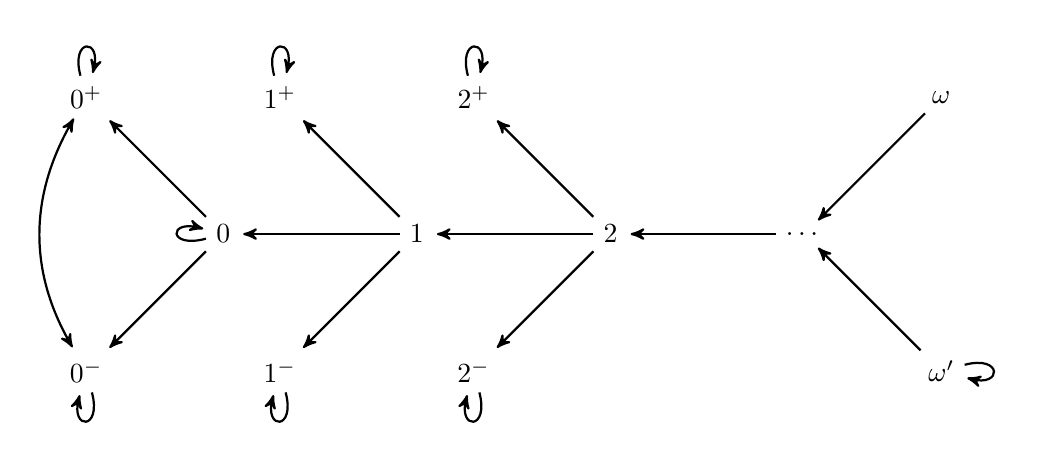
\begin{tikzpicture}[>=stealth',shorten >=1pt,auto,node distance=7em,thick]

      \node (0) {$0$};
      \node (0+) [above left of=0] {$0^+$};
      \node (0-) [below left of=0] {$0^-$};
      \node (1) [right of=0] {$1$};
      \node (1+) [above left of=1] {$1^+$};
      \node (1-) [below left of=1] {$1^-$};
      \node (2) [right of=1] {$2$};
      \node (2+) [above left of=2] {$2^+$};
      \node (2-) [below left of=2] {$2^-$};
      \node (3) [right of=2] {\ldots};
      \node (omega) [above right of=3] {$\omega$};
      \node (omega') [below right of=3] {$\omega'$};

      \path[every node/.style={font=\sffamily\small},->]
        (0) edge [loop left] node {} (0)
            edge node {} (0+)
            edge node {} (0-)
        (0+) edge [loop above] node  {} (0+)
            edge [<->,bend right] node {} (0-)
        (0-) edge [loop below] node  {} (0-)
        (1) edge node {} (0)
            edge node {} (1+)
            edge node {} (1-)
        (1+) edge [loop above] node {} (1+)
        (1-) edge [loop below] node {} (1-)
        (2) edge node {} (1)
            edge node {} (2+)
            edge node {} (2-)
        (2+) edge [loop above] node {} (2+)
        (2-) edge [loop below] node {} (2-)
        (3) edge node {} (2)
        (omega) edge node {} (3)
        (omega') edge node {} (3)
            edge [loop right] node {} (omega');
    \end{tikzpicture}
    \caption{The model $\kModel$, omitting implied transitive edges.}\label{model-caterpillar}
\end{figure}

To show that $\kPModel{\omega}$ and $\kPModel{\omega'}$ are indistinguishable by the refinement modal logic we show that $\kPModel{\omega} \bisimref[n] \kPModel{\omega'}$ for all $n \in \naturals$. To do so we first show that $\kPModel{\omega}$ and $\kPModel{\omega'}$ are mutual refinements.

That $\kPModel{\omega} \refines \kPModel{\omega'}$ is trivial, as $\omega$ is the same as $\omega'$ except for the reflexive edge, so we need only show that $\kPModel{\omega'} \refines \kPModel{\omega}$.

Let $\refinement \subseteq \kStates \times \kStates$ be defined as follows:
$$
\refinement = \{(\kStateS, \kStateS) \mid \kStateS \in \kStates\} \cup
\{(0, n), (n, 0), (0^+, n^+), (0^-, n^-), (\omega, n), (\omega', n) \mid n \in \naturals\} \cup
\{(0, \omega), (0, \omega'), (\omega, \omega')\}
$$

% TODO
We show that $\refinement$ satisfies {\bf atoms-$\atomP$} and {\bf back} for every $(\kStateS, \kStateSP) \in \refinement$.

\paragraph{atoms}
Trivial.

\paragraph{back-$a$}
Consider $(\kStateS, \kStateS) \in \refinement$ and let $\kStateT \in \kSuccessors{}{\kStateS}$. Then $(\kStateT, \kStateT) \in \refinement$.

Consider $(0, n) \in \refinement$ and let $\kStateT \in \kSuccessors{}{n}$. 
Suppose that $\kStateT = m$ for $m \in \naturals$. 
Then $0 \in \kSuccessors{}{0}$ and $(0, m) \in \refinement$.
Suppose that $\kStateT = m^+$ for $m \in \naturals$.
Then $0^+ \in \kSuccessors{}{0}$ and $(0^+, m^+) \in \refinement$.
Suppose that $\kStateT = m^-$ for $m \in \naturals$.
Then $0^- \in \kSuccessors{}{0}$ and $(0^-, m^-) \in \refinement$.

Consider $(n, 0) \in \refinement$ and let $\kStateT \in \kSuccessors{}{0}$.
Then $\kStateT \in \kSuccessors{}{n}$ and $(\kStateT, \kStateT) \in \refinement$.

Consider $(0^+, n^+) \in \refinement$ and let $\kStateT \in \kSuccessors{}{n^+}$. 
Then $t = n^+$, $0^+ \in \kSuccessors{}{0^+}$ and $(0^+, n^+) \in \refinement$.

Consider $(0^-, n^-) \in \refinement$ and let $\kStateT \in \kSuccessors{}{n^-}$. 
Then $t = n^-$, $0^- \in \kSuccessors{}{0^-}$ and $(0^-, n^-) \in \refinement$.

Consider $(0, \omega) \in \refinement$ and let $\kStateT \in \kSuccessors{}{\omega}$. 
This case follows the same reasoning as for the case for $(0, n) \in \refinement$.

Consider $(0, \omega') \in \refinement$ and let $\kStateT \in \kSuccessors{}{\omega}$. 
Suppose that $t \neq \omega'$. 
This case follows the same reasoning as for the case for $(0, n) \in \refinement$. 
Suppose that $t = \omega'$. 
Then $0 \in \kSuccessors{}{0}$ and $(0, \omega') \in \refinement$.

Consider $(\omega, \omega') \in \refinement$ and let $\kStateT \in \kSuccessors{}{\omega'}$. 
Suppose that $t \neq \omega'$. 
Then $t \in \kSuccessors{}{\omega}$ and $(t, t) \in \refinement$. 
Suppose that $t = \omega'$. 
Then $0 \in \kSuccessors{}{\omega}$ and $(0, \omega') \in \refinement$.

Consider $(\omega, n) \in \refinement$ and let $\kStateT \in \kSuccessors{}{n}$.
Then $\kStateT \in \kSuccessors{}{\omega}$ and $(t, t) \in \refinement$.

Consider $(\omega', n) \in \refinement$ and let $\kStateT \in \kSuccessors{}{n}$.
Then $\kStateT \in \kSuccessors{}{\omega'}$ and $(t, t) \in \refinement$.

We show that $\kPModel{\omega} \bisimref[n] \kPModel{\omega'}$ for every $n \in \naturals$. 
To do so we show the following intermediate results:

\begin{enumerate}
    \item $\kPModel{i} \bisimref[n] \kPModel{j}$ for $i, j, n \in \naturals$ where $i, j \geq n$.

    By induction on $n \in \naturals$.

    Suppose that $n = 0$. 
    From above, $\kPModel{i} \refines \kPModel{0} \refines \kPModel{j}$ and $\kPModel{i} \simulates \kPModel{0} \simulates \kPModel{j}$ so we have that $\kPModel{i} \bisimref[0] \kPModel{j}$.

    Suppose that $n > 0$.

    \paragraph{mutual refinements}

    From above, $\kPModel{i} \refines \kPModel{0} \refines \kPModel{j}$
    and $\kPModel{i} \simulates \kPModel{0} \simulates \kPModel{j}$.

    \paragraph{forth}

    Let $k^* \in \kSuccessors{}{i}$.
    Suppose that $k^* = k$ where $k \in \naturals$ and $k \geq n - 1$.
    Then from the induction hypothesis $\kPModel{k} \bisimilar [n-1] \kPModel{j - 1}$.
    Suppose that $k^* = k$ where $k \in \naturals$ and $k < n - 1$.
    Then $k < n - 1 < j$ so $k \in \kSuccessors{}{j}$ and we trivially have that $\kPModel{k} \bisimilar \kPModel{k}$.
    Suppose that $k^* = 0^+$.
    Then $0^+ \in \kSuccessors{}{j}$ and we trivially have that $\kPModel{0^+} \bisimilar \kPModel{0^+}$.
    Suppose that $k^* = k^+$ where $k \in \naturals$ and $k > 0$.
    Then $j^+ \in \kSuccessors{}{j}$ and as $j \geq n > 0$ we trivially have that $\kPModel{k^+} \bisimilar \kPModel{k^+}$.
    Suppose that $k^* = k^-$ for $k \in \naturals$. This follows from similar reasoning to the case where $k^* = k^+$.

    \paragraph{back}

    Symmetrical reasoning to {\bf forth}.

    \item $\kPModel{n} \bisimref[n] \kPModel{\omega'}$ for $n \in \naturals$.

    By induction on $n$.

    Suppose that $n = 0$. 
    From above, $\kPModel{n} \refines \kPModel{0} \refines \kPModel{\omega'}$ and $\kPModel{n} \simulates \kPModel{\omega'}$ so we have that $\kPModel{0} \bisimref[0] \kPModel{\omega'}$.

    Suppose that $n > 0$.

    \paragraph{mutual refinements}

    From above, $\kPModel{n} \refines \kPModel{0} \refines \kPModel{\omega'}$ and $\kPModel{n} \simulates \kPModel{\omega'}$.

    \paragraph{forth}

    Let $k \in \kSuccessors{}{n}$. 
    Then $k \in \kSuccessors{}{\omega'}$ and we trivially have that $\kPModel{k} \bisimilar \kPModel{k}$.

    \paragraph{back}

    Let $k \in \kSuccessors{}{\omega'}$. 
    Suppose that $k = \omega'$. 
    Then $n - 1 \in \kSuccessors{}{n}$ and by the induction hypothesis $\kPModel{n - 1} \bisimilar{n - 1} \kPModel{\omega'}$.
    Suppose that $k \neq \omega'$ and $k < n$. Then $k \in \kSuccessors{}{n}$ and we trivially have that $\kPModel{k} \bisimilar \kPModel{k}$.
    Suppose that $k \geq n$. Then $n - 1 \in \kSuccessors{}{n}$ and from above we have that $\kPModel{k} \bisimref[n - 1] \kPModel{n - 1}$.
    
    \item $\kPModel{\omega} \bisimref[n] \kPModel{\omega'}$ for $n \in \naturals$.

    By induction on $n$.

    Suppose that $n = 0$. 
    From above $\kPModel{\omega} \refines \kPModel{\omega'}$ and  $\kPModel{\omega} \simulates \kPModel{\omega'}$ so we have that $\kPModel{\omega} \bisimref[0] \kPModel{\omega'}$.

    Suppose that $n > 0$.

    \paragraph{mutual refinements}

    From above $\kPModel{\omega} \refines \kPModel{\omega'}$ and  $\kPModel{\omega} \simulates \kPModel{\omega'}$.

    \paragraph{forth}

    Let $k \in \kSuccessors{}{\omega}$.
    Then $k \in \kSuccessors{}{\omega'}$ and we trivially have that $\kPModel{k} \bisimilar \kPModel{k}$.

    \paragraph{back}

    Let $k \in \kSuccessors{}{\omega'}$.
    Suppose that $k = \omega'$.
    Then $n - 1 \in \kSuccessors{}{\omega}$ and from above we have that $\kPModel{n - 1} \bisimref[n - 1] \kPModel{\omega'}$.
    Suppose that $k \neq \omega'$.
    Then $k \in \kSuccessors{}{\omega}$ and we trivially have that $\kPModel{k} \bisimilar \kPModel{k}$.
\end{enumerate}

Therefore $\kPModel{\omega} \bisimref[n] \kPModel{\omega'}$ for every $n \in \naturals$ and so $\kPModel{\omega}$ and $\kPModel{\omega'}$ are indistinguishable to refinement modal logic.

We next show that the states $\kPModel{\omega}$ and $\kPModel{\omega'}$ are distinguishable by the tangled modal logic formula $\tangle \{\possible \necessary \atomP, \possible \necessary \neg \atomP\}$.
We first note that in the modal $\mu$-calculus we have that $\tangle \{\possible \necessary \atomP, \possible \necessary \neg \atomP\} \equiv \gfp{\varX} (\possible (\varX \land \possible \necessary \atomP) \land \possible (\varX \land \possible \necessary \neg \atomP))$.
We proceed with model checking using the modal $\mu$-calculus.

For any assignment $\kAssignment$ we have the following:
\begin{eqnarray*}
    \interpretation[\kAssignment]{\atomP} &=& \{n, n^+ \mid n \in \naturals\} \cup \{\omega, \omega'\}\\
    \interpretation[\kAssignment]{\necessary \atomP} &=& \{n^+ \mid n \in \naturals, n > 0\}\\
    \interpretation[\kAssignment]{\possible \necessary \atomP} &=& \{n, n^+ \mid n \in \naturals, n > 0\} \cup \{\omega, \omega'\}\\
    \interpretation[\kAssignment]{\neg \atomP} &=& \{n^- \mid n \in \naturals\}\\
    \interpretation[\kAssignment]{\necessary \neg \atomP} &=& \{n^- \mid n \in \naturals, n > 0\}\\
    \interpretation[\kAssignment]{\possible \necessary \neg \atomP} &=& \{n, n^- \mid n \in \naturals, n > 0\} \cup \{\omega, \omega'\}
\end{eqnarray*}

For any assignment $\kAssignment$ where $\kAssignment(\varX) = \kStates$ we have the following:
\begin{eqnarray*}
    \interpretation[\kAssignment]{\varX} &=& \kStates\\
    \interpretation[\kAssignment]{\varX \land \possible \necessary \atomP} &=& \{n, n^+ \mid n \in \naturals, n > 0\} \cup \{\omega, \omega'\}\\
    \interpretation[\kAssignment]{\possible (\varX \land \possible \necessary \atomP)} &=& \{n, n^+ \mid n \in \naturals, n > 0\} \cup \{\omega, \omega'\}\\
    \interpretation[\kAssignment]{\varX \land \possible \necessary \neg \atomP} &=& \{n, n^- \mid n \in \naturals, n > 0\} \cup \{\omega, \omega'\}\\
    \interpretation[\kAssignment]{\possible (\varX \land \possible \necessary \neg \atomP)} &=& \{n, n^- \mid n \in \naturals, n > 0\} \cup \{\omega, \omega'\}\\
    \interpretation[\kAssignment]{\possible (\varX \land \possible \necessary \atomP) \land \possible (\varX \land \possible \necessary \neg \atomP)} &=& \{n \mid n \in \naturals, n > 0\} \cup \{\omega, \omega'\}
\end{eqnarray*}

For any assignment $\kAssignment$ where $\kAssignment(\varX) = \{n \mid n \in \naturals, n > m\} \cup \{\omega, \omega'\}$ for some $m \in \naturals$ we have the following:
\begin{eqnarray*}
    \interpretation[\kAssignment]{\varX} &=& \{n \mid n \in \naturals, n > m\} \cup \{\omega, \omega'\}\\
    \interpretation[\kAssignment]{\varX \land \possible \necessary \atomP} &=& \{n \mid n \in \naturals, n > m\} \cup \{\omega, \omega'\}\\
    \interpretation[\kAssignment]{\possible (\varX \land \possible \necessary \atomP)} &=& \{n \mid n \in \naturals, n > m + 1\} \cup \{\omega, \omega'\}\\
    \interpretation[\kAssignment]{\varX \land \possible \necessary \neg \atomP} &=& \{n \mid n \in \naturals, n > m\} \cup \{\omega, \omega'\}\\
    \interpretation[\kAssignment]{\possible (\varX \land \possible \necessary \neg \atomP)} &=& \{n \mid n \in \naturals, n > m + 1\} \cup \{\omega, \omega'\}\\
    \interpretation[\kAssignment]{\possible (\varX \land \possible \necessary \atomP) \land \possible (\varX \land \possible \necessary \neg \atomP)} &=& \{n \mid n \in \naturals, n > m + 1\} \cup \{\omega, \omega'\}
\end{eqnarray*}

For any assignment $\kAssignment$ where $\kAssignment(\varX) = \{\omega, \omega'\}$ for some $m \in \naturals$ we have the following:
\begin{eqnarray*}
    \interpretation[\kAssignment]{\varX} &=& \{\omega, \omega'\}\\
    \interpretation[\kAssignment]{\varX \land \possible \necessary \atomP} &=& \{\omega, \omega'\}\\
    \interpretation[\kAssignment]{\possible (\varX \land \possible \necessary \atomP)} &=& \{\omega'\}\\
    \interpretation[\kAssignment]{\varX \land \possible \necessary \neg \atomP} &=& \{\omega, \omega'\}\\
    \interpretation[\kAssignment]{\possible (\varX \land \possible \necessary \neg \atomP)} &=& \{\omega'\}\\
    \interpretation[\kAssignment]{\possible (\varX \land \possible \necessary \atomP) \land \possible (\varX \land \possible \necessary \neg \atomP)} &=& \{\omega'\}
\end{eqnarray*}

Therefore for any assignment $\kAssignment$ we have that: $$\interpretation[\kAssignment]{\gfp{\varX} (\possible (\varX \land \possible \necessary \atomP) \land \possible (\varX \land \possible \necessary \neg \atomP))} = \{\omega'\}$$

Therefore $\kPModel{\omega'} \entails \gfp{\varX} (\possible (\varX \land \possible \necessary \atomP) \land \possible (\varX \land \possible \necessary \neg \atomP))$, 
but $\kPModel{\omega} \nentails \gfp{\varX} (\possible (\varX \land \possible \necessary \atomP) \land \possible (\varX \land \possible \necessary \neg \atomP))$
and so $\kPModel{\omega}$ and $\kPModel{\omega'}$ are distinguishable by the tangled modal logic.

\end{proof}

\begin{corollary}
The logic \logicRmlKF{} is strictly less expressive than \logicMuKF{}.
\end{corollary}

    \chapter{Arbitrary action model logic}\label{aaml}

\section{Syntax and semantics}\label{aaml-semantics}

In this section we introduce the syntax and semantics of the arbitrary action model logic.
Like our treatment of \logicRml{}, we consider \logicAaml{} in different settings, including \classK{}, \classKFF{}, and \classS{}.
The definitions that we give here generalise to these different settings.
Unlike our treatment of \logicRml{}, we don't give any semantic results that are common to all of these settings.
As our main results in \logicAaml{} are to show that the action model quantifiers of \logicAaml{} are equivalent to the refinement quantifiers of \logicRml{} in the settings we consider, all of the semantic results from \logicRml{} also apply to \logicAaml{} in these settings.
For the same reason we use the same syntax for action model quantifiers and refinement quantifiers.

We begin with a definition of the syntax of \logicAaml{}.
As in action model logic, the syntax of \logicAaml{} is parameterised by a class of Kripke models, \classC{}, and a set of action signatures, \aSignatureFamily{}.

\begin{definition}[Language of arbitrary action model logic]
Let \aSignatureFamily{} be a non-empty, countable set of action signatures.
The {\em language of arbitrary action model logic} with action signatures \aSignatureFamily{}, $\langAaml(\aSignatureFamily)$, is inductively defined as:
$$
\phi ::= 
    \atomP \mid
    \lnot \phi \mid
    \phi \land \phi \mid
    \necessaryA \phi \mid
    \actionA{\aSignature \aStatesT, \phi, \dots, \phi} \phi \mid
    \allactsBs \phi
$$
where $\atomP \in \atoms$, $\agentA \in \agents$, $\agentsB \subseteq \agents$, $\aSignatureAndTuple \in \aSignatureFamily$, $\aStatesT \subseteq \aStates$, and the number of parameters to a given action signature $\aSignature$ is determined by the number of designated actions in the action signature.
\end{definition}

We use all of the standard abbreviations from action model logic and refinement modal logic.

The formula $\allacts \phi$ may be read as ``every action model results in $\phi$ becoming true'' and the formula $\someacts \phi$ may be read as ``some action model results in $\phi$ becoming true''.

The use of the subscript $\agentsB$ in the quantifiers $\allactsBs$ and $\someactsBs$ restricts the action models under consideration to action models that result in a $\agentsB$-refinement of the original Kripke model.
So the formula $\allactsBs \phi$ may be reas as ``every action model results in $\phi$ becoming true if it results in a $\agentsB$-refinement'' and the formula $\someactsBs \phi$ may be read as ``some action model results in $\phi$ becoming true and results in a $\agentsB$-refinement''.
This addition is mostly for the purposes of showing a full correspondence between action model quantifiers and refinement quantifiers.
Although we do not consider it in greater detail here, the notion of restricting the results of executing action models to $\agentsB$-refinements seems like it would be useful.
For example, $\agentsB$-refinements can be partially characterised as those Kripke models that preserve the truth of $\agentsB$-positive formulas, restricting the learning of new information to agents in $\agentsB$.
So an alternative reading of the formula $\allactsBs \phi$ may be ``every action model where only agents in $\agentsB$ learn new information results in $\phi$ becoming true'' and an alternative reading of the formula $\someactsBs \phi$ may be ``some action model where only agents in $\agentsB$ learn new information results in $\phi$ becoming true''.

We define the semantics of \logicAaml{}.

\begin{definition}[Semantics of arbitrary action model logic]
Let \classC{} be a class of Kripke models and let \aSignatureFamily{} be a non-empty, countable set of action signatures, let $\phi \in \langAaml(\aSignatureFamily)$, and let $\kPModelAndTuple{\kStateS} \in \classC$ be a pointed Kripke model.
The interpretation of the formula $\phi$ in the logic \logicAamlC{} on the pointed Kripke model $\kPModel{\kStateS}$ is the same as its interpretation in action model logic, defined in Definition~\ref{aml-semantics}, with the additional inductive case:
$$
\begin{array}{lcl}
    \kPModel{\kStateS} \entails \allactsBs \phi & \text{ iff } & \text{for every } \aPModel{\aStateS} \in \aSignatureFamily \text{ if } \kPModel{\kStateS} \entails \aPrecondition(\aStateS) \text{ and } \kPModel{\kStateS} \simulatesBs \kPModel{\kStateS} \exec \aPModel{\aStateS}\\&&\quad \text{ then } \kPModel{\kStateS} \exec \aPModel{\aStateS} \entails \phi
\end{array}
$$
\end{definition}

We are interested in the following variants of arbitrary action model logic:
\begin{itemize}
    \item \logicAamlK{} interpreted over the class of \classK{} Kripke frames and the language of arbitrary action model logic $\langAaml(\classK)$ with action signatures defined on the class of finite \classK{} Kripke frames.
    \item \logicAamlKFF{} interpreted over the class of \classKFF{} Kripke frames and the language of arbitrary action model logic $\langAaml(\classKFF)$ with action signatures defined on the class of finite \classKFF{} Kripke frames.
    \item \logicAamlS{} interpreted over the class of \classS{} Kripke frames and the language of arbitrary action model logic $\langAaml(\classS)$ with action signatures defined on the class of finite \classS{} Kripke frames.
\end{itemize}

We note that by Proposition~\ref{action-models-refinements} the result of executing any action model is a $\agents$-refinement, so the action model quantifiers $\allactsAs$ and $\someactsAs$, abbreviated as $\allacts$ and $\someacts$ respectively, correspond to unrestricted action model quantification.
Given this we can observe that the semantics of the action model quantifiers $\allacts$ and $\someacts$ are defined similarly to the semantics of the public announcement quantifier of \logicApal{}.
One notable difference is that whilst \logicApal{} permits public announcements of formulas containing public announcement quantifiers, the public announcement quantifiers do not quantify over public announcements that themselves contain quantifiers, whereas the action model quantifier of \logicAaml{} makes no such restriction.
We will show in the following sections that such a restriction is unnecessary in the settings that we consider; the logics \logicAamlK{}, \logicAamlKFF{}, and \logicAamlS{} are expressively equivalent to their underlying modal logics, \logicK{}, \logicKFF{}, and \logicS{} respectively, so any action model containing quantifiers is equivalent to an action model without quantifiers.

\todo[inline]{Example of \logicAaml{}}

In the following sections we show that the action model quantifiers of \logicAaml{} are equivalent to the refinement quantifiers of \logicRml{} in the settings of \classK{}, \classKFF{}, and \classS{}.
We show the equivalence by showing that if there exists a refinement where a given formula is satisfied then we can construct a finite action model that results in that formula being satisfied.
The converse we have already shown; if there exists a (possibly infinite) action model that results in a given formula being satisfied then by Proposition~\ref{action-models-refinements} the result of executing the action model is itself a refinement, so there exists a refinement where the formula is satisfied.
We rely heavily on results from action model logic and \logicRml{}, particularly the axioms from both, so we find it useful to define a logic, which we call refinement action model logic (\logicRaml{}), that extends action model logic with refinement quantifiers.

\begin{definition}[Semantics of refinement action model logic]
Let \classC{} be a class of Kripke models and let \aSignatureFamily{} be a non-empty, countable set of action signatures, let $\phi \in \langAaml(\aSignatureFamily)$, and let $\kPModelAndTuple{\kStateS} \in \classC$ be a pointed Kripke model.
The interpretation of the formula $\phi$ in the logic \logicRamlC{} on the pointed Kripke model $\kPModel{\kStateS}$ is the same as its interpretation in action model logic, defined in Definition~\ref{aml-semantics}, with the additional inductive case:
$$
\begin{array}{lcl}
    \kPModel{\kStateS} \entails \allactsBs \phi & \text{ iff } & \text{for every } \kPModelP{\kStateSP} \in \classC \text{ if } \kPModel{\kStateS} \simulatesBs \kPModelP{\kStateSP} \text{ then } \kPModelP{\kStateSP} \entails \phi
\end{array}
$$
\end{definition}

As with \logicAaml{} we are interested in the following variants of refinement action model logic:
\begin{itemize}
    \item \logicRamlK{} interpreted over the class of \classK{} Kripke frames and the language of arbitrary action model logic $\langAaml(\classK)$ with action signatures defined on the class of finite \classK{} Kripke frames.
    \item \logicRamlKFF{} interpreted over the class of \classKFF{} Kripke frames and the language of arbitrary action model logic $\langAaml(\classKFF)$ with action signatures defined on the class of finite \classKFF{} Kripke frames.
    \item \logicRamlS{} interpreted over the class of \classS{} Kripke frames and the language of arbitrary action model logic $\langAaml(\classS)$ with action signatures defined on the class of finite \classS{} Kripke frames.
\end{itemize}

In the following sections we will show that results from action model logic and \logicRml{} apply to the combined logic \logicRaml{}, and use these results to show that formulas of \langAaml{} have the same interpretation in both \logicAaml{} and \logicRaml{}.

\section{K}

\begin{definition}[Axiomatisation \axiomAamlK{}]
The axiomatisation \axiomAamlK{} is a substitution schema consisting of the axioms and rules of \axiomAmlK{} and the axioms and rules of \axiomRmlK{}.
\end{definition}

\begin{theorem}\label{aaml-k-sound-complete}
The axiomatisation \axiomRmlK{} is sound and strongly complete with respect to the semantics of the logic \logicAamlK{}.
\end{theorem}

\begin{proof}[Proof (Sketch)]
Soundness of the axioms and rules from \axiomAmlK{} and \axiomRmlK{} follow from the same reasoning used to show that they are sound in \logicAmlK{} and \logicRmlK{} respectively.
Strong completeness follows from similar reasoning as in the proof of strong completeness of \axiomRmlK{} in Lemma~\ref{rml-k-sound-complete}.
We note that the axioms of \axiomAmlK{} form a set of reduction axioms that can be used to provably translate any formula containing action model operators but not refinement quantifiers into an equivalent modal formula.
Likewise the axioms of \axiomRmlK{} form a set of reduction axioms that can be used to provably translate any formula containing refinement quantifiers but not action model operators into an equivalent modal formula.
These methods can be combined to provably translate any formula containing action model operators and refinement quantifiers into an equivalent modal formula, by iteratively translating subformulas containing action model operators but not refinement quantifiers using the former method, and subformulas containing refinement quantifiers but not action model operators using the latter method.
\end{proof}

\begin{corollary}\label{aaml-k-expressive-equivalence}
The logic \logicAamlK{} is expressively equivalent to the logic \logicK{}.
\end{corollary}

\begin{corollary}
The logic \logicAamlK{} is compact.
\end{corollary}

\begin{corollary}
The satisfiability problem for the logic \logicAamlK{} is decidable.
\end{corollary}

\begin{lemma}\label{aaml-k-choice}
Let $\agentsB \subseteq \agents$, 
let $\phi = \alpha \lor \beta \in \langAaml$, and 
let $\aPModel[\alpha]{\aStatesT[\alpha]} \in \classAmK$ and $\aPModel[\beta]{\aStatesT[\beta]} \in \classAmK$ be action models such that 
$\entails \actionA{\aPModel[\alpha]{\aStatesT[\alpha]}} \alpha$, 
$\entails \actionE{\aPModel[\alpha]{\aStatesT[\alpha]}} \alpha \iff \someactsBs \alpha$, 
$\entails \actionA{\aPModel[\beta]{\aStatesT[\beta]}} \beta$,
$\entails \actionE{\aPModel[\beta]{\aStatesT[\beta]}} \beta \iff \someactsBs \beta$,
for every $\aStateT[\alpha] \in \aStatesT[\alpha]$, $\kPModel{\kStateS} \in \classK$ if $\kPModel{\kStateS} \entails \aPrecondition[\alpha](\aStateT[\alpha])$ then $\kPModel{\kStateS} \simulatesBs \kPModel{\kStateS} \exec \aPModel[\alpha]{\aStateT[\alpha]}$, and
for every $\aStateT[\beta] \in \aStatesT[\beta]$, $\kPModel{\kStateS} \in \classK$ if $\kPModel{\kStateS} \entails \aPrecondition[\beta](\aStateT[\beta])$ then $\kPModel{\kStateS} \simulatesBs \kPModel{\kStateS} \exec \aPModel[\beta]{\aStateT[\beta]}$.
Then there exists an action model $\aPModel{\aStatesT} \in \classAmK$ such that 
$\entails \actionA{\aPModel{\aStatesT}} \phi$,
$\entails \actionE{\aPModel{\aStatesT}} \phi \iff \someactsBs \phi$, and
for every $\aStateT \in \aStatesT$, $\kPModel{\kStateS} \in \classK$ if $\kPModel{\kStateS} \entails \aPrecondition(\aStateT)$ then $\kPModel{\kStateS} \simulatesBs \kPModel{\kStateS} \exec \aPModel{\aStateT}$.
\end{lemma}

\begin{proof}
Without loss of generality we assume that $\aModel[\alpha]$ and $\aModel[\beta]$ are disjoint.
We construct the action model $\aPModel{\aStatesT} = \aPModel[\alpha]{\aStatesT[\alpha]} \choice \aPModel[\beta]{\aStatesT[\beta]} = \aPModelTuple{\aStatesT}$ where the disjoint union of action models is defined in Definition~\ref{aml-choice}.  
As $\aModel$ is formed by the disjoint union of $\aModel[\alpha]$ and $\aModel[\beta]$ we note that each state of $\aModel[\alpha]$ and $\aModel[\beta]$ is bisimilar to the corresponding state in $\aModel$.

We first show that for every $\aStateT \in \aStatesT$, $\kPModel{\kStateS} \in \classK$ if $\kPModel{\kStateS} \entails \aPrecondition(\aStateT)$ then $\kPModel{\kStateS} \simulatesBs \kPModel{\kStateS} \exec \aPModel{\aStateT}$.
Let $\gamma \in \{\alpha, \beta\}$, $\aStateT[\gamma] \in \aStatesT[\gamma] \subseteq \aStatesT$, and $\kPModel{\kStateS} \in \classK$ such that $\kPModel{\kStateS} \entails \aPrecondition(\aStateT[\gamma])$.
By construction $\aPrecondition(\aStateT[\gamma]) = \aPrecondition[\gamma](\aStateT[\gamma])$ and so $\kPModel{\kStateS} \entails \aPrecondition[\gamma](\aStateT[\gamma])$. 
By hypothesis then $\kPModel{\kStateS} \simulatesBs \kPModel{\kStateS} \exec \aPModel[\gamma]{\aStateT[\gamma]}$.
From above $\aPModel{\aStateT[\gamma]} \bisimilar \aPModel[\gamma]{\aStateT[\gamma]}$ and so from Proposition~\ref{action-bisimulation-results} we have that $\kPModel{\kStateS} \exec \aPModel{\aStateT[\gamma]} \bisimilar \kPModel{\kStateS} \exec \aPModel[\gamma]{\aStateT[\gamma]}$.
From Corollary~\ref{bisimilar-refinement} and Proposition~\ref{refinements-preorder} we have that $\kPModel{\kStateS} \simulatesBs \kPModel{\kStateS} \exec \aPModel{\aStateT[\gamma]}$.

We next show that $\entails \actionA{\aPModel{\aStatesT}} \phi$.
\begin{eqnarray}
    &&\entails \actionA{\aPModel[\alpha]{\aStatesT[\alpha]}} \alpha \land \actionA{\aPModel[\beta]{\aStatesT[\beta]}} \beta \label{aaml-k-choice-1}\\
    &&\entails \actionA{\aPModel{\aStatesT[\alpha]}} \alpha \land \actionA{\aPModel{\aStatesT[\beta]}} \beta \label{aaml-k-choice-2}\\
    &&\entails \actionA{\aPModel{\aStatesT[\alpha]}} (\alpha \lor \beta) \land \actionA{\aPModel{\aStatesT[\beta]}} (\alpha \lor \beta) \label{aaml-k-choice-3}\\
    &&\entails \actionA{\aPModel{\aStatesT}} (\alpha \lor \beta) \label{aaml-k-choice-4}
\end{eqnarray}
(\ref{aaml-k-choice-1}) follows from hypothesis;
(\ref{aaml-k-choice-2}) follows from the above note that $\aPModel[\alpha]{\aStatesT[\alpha]} \bisimilar \aPModel{\aStatesT[\alpha]}$ and $\aPModel[\beta]{\aStatesT[\beta]} \bisimilar \aPModel{\aStatesT[\beta]}$ and Proposition~\ref{aml-bisimilar-actions};
(\ref{aaml-k-choice-3}) follows from propositional disjunction introduction; and
(\ref{aaml-k-choice-4}) follows from \axiomAamlK{} axiom {\bf AU}, as $\aStatesT = \aStatesT[\alpha] \cup \aStatesT[\beta]$.

Finally we show that $\entails \actionE{\aPModel{\aStatesT}} \phi \iff \someactsBs \phi$.
\begin{eqnarray}
    &&\entails \someactsBs (\alpha \lor \beta) \implies (\someactsBs \alpha \lor \someactsBs \beta) \label{aaml-k-choice-5}\\
    &&\entails \someactsBs (\alpha \lor \beta) \implies (\actionE{\aPModel[\alpha]{\aStatesT[\alpha]}} \alpha \land \actionE{\aPModel[\beta]{\aStatesT[\beta]}} \beta) \label{aaml-k-choice-6}\\
    &&\entails \someactsBs (\alpha \lor \beta) \implies (\actionE{\aPModel{\aStatesT[\alpha]}} \alpha \land \actionE{\aPModel{\aStatesT[\beta]}} \beta) \label{aaml-k-choice-7}\\
    &&\entails \someactsBs (\alpha \lor \beta) \implies (\actionE{\aPModel{\aStatesT[\alpha]}} (\alpha \lor \beta) \land \actionE{\aPModel{\aStatesT[\beta]}} (\alpha \lor \beta)) \label{aaml-k-choice-8}\\
    &&\entails \someactsBs (\alpha \lor \beta) \implies \actionE{\aPModel{\aStatesT}} (\alpha \lor \beta) \label{aaml-k-choice-9}
\end{eqnarray}
(\ref{aaml-k-choice-5}) follows from \axiomAamlK{} axiom {\bf R};
(\ref{aaml-k-choice-6}) follows from hypothesis;
(\ref{aaml-k-choice-7}) follows from the above note that $\aPModel[\alpha]{\aStatesT[\alpha]} \bisimilar \aPModel{\aStatesT[\alpha]}$ and $\aPModel[\beta]{\aStatesT[\beta]} \bisimilar \aPModel{\aStatesT[\beta]}$ and Proposition~\ref{aml-bisimilar-actions};
(\ref{aaml-k-choice-8}) follows from propositional disjunction introduction; and
(\ref{aaml-k-choice-9}) follows from \axiomAamlK{} axiom {\bf AU}, as $\aStatesT = \aStatesT[\alpha] \cup \aStatesT[\beta]$.

The converse, that $\entails \actionE{\aPModel{\aStatesT}} \phi \implies \someactsBs \phi$ follows from a simple semantic argument.
Let $\kPModel{\kStateS} \in \classK$ and suppose that $\kPModel{\kStateS} \entails \actionE{\aPModel{\aStatesT}} \phi$.
Then there exists $\aStateS \in \aStatesT$ such that $\kPModel{\kStateS} \entails \aPrecondition(\aStateS)$ and $\kPModel{\kStateS} \exec \aPModel{\aStateS} \entails \phi$.
From above, $\kPModel{\kStateS} \simulatesBs \kPModel{\kStateS} \exec \aPModel{\aStateS}$, so $\kPModel{\kStateS} \entails \someactsBs \phi$.
Therefore $\entails \actionE{\aPModel{\aStatesT}} \phi \implies \someactsBs \phi$.
\end{proof}

\begin{lemma}\label{aaml-k-covers}
Let $\agentsB, \agentsC \subseteq \agents$, 
let $\phi = \pi \land \bigwedge_{\agentC \in \agentsC} \coverC \Gamma_\agentC \in \langAaml$ where $\pi \in \langPl$, and 
for every $\agentC \in \agentsC$, $\gamma \in \agentsC$
let $\aPModelAndTuple[\gamma]{\aStatesT[\gamma]} \in \classAmK$ be a $\agentsB$-action model such that 
$\entails \actionA{\aPModel[\gamma]{\aStatesT[\gamma]}} \gamma$,
$\entails \actionE{\aPModel[\gamma]{\aStatesT[\gamma]}} \gamma \iff \someactsBs \gamma$, and
for every $\aStateT[\gamma] \in \aStatesT[\gamma]$, $\kPModel{\kStateS} \in \classK$ if $\kPModel{\kStateS} \entails \aPrecondition[\gamma](\aStateT[\gamma])$ then $\kPModel{\kStateS} \simulatesBs \kPModel{\kStateS} \exec \aPModel[\gamma]{\aStateT[\gamma]}$.
Then there exists a $\agentsB$-action model $\aPModel{\aStatesT} \in \classAmK$ such that 
$\entails \actionA{\aPModel{\aStatesT}} \phi$, and 
$\entails \actionE{\aPModel{\aStatesT}} \phi \iff \someactsBs \phi$.
for every $\aStateT \in \aStatesT$, $\kPModel{\kStateS} \in \classK$ if $\kPModel{\kStateS} \entails \aPrecondition(\aStateT)$ then $\kPModel{\kStateS} \simulatesBs \kPModel{\kStateS} \exec \aPModel{\aStateT}$.
\end{lemma}

\begin{proof}
Without loss of generality we assume that each $\aModel[\gamma]$ for every $\agentC \in \agentsC$, $\gamma \in \Gamma_\agentC$ is disjoint.

We construct the action model $\aPModelAndTuple{\aStateTest}$ where:
\begin{eqnarray*}
    \aStates &=& \{\aStateTest, \aStateSkip\} \cup \bigcup_{\agentC \in \agentsC, \gamma \in \Gamma_\agentC} \aStates[\gamma]\\
    \aAccessibilityA &=& \{(\aStateTest, \aStateT[\gamma]) \mid \gamma \in \Gamma_\agentA, \aStateT[\gamma] \in \aStatesT[\gamma]\} \cup \{(\aStateSkip, \aStateSkip)\} \cup \bigcup_{\agentC \in \agentsC, \gamma \in \Gamma_\agentC} \aAccessibilityA[\gamma] \text{ for } \agentA \in \agentsC\\
    \aAccessibilityA &=& \{(\aStateTest, \aStateSkip), (\aStateSkip, \aStateSkip)\} \cup \bigcup_{\agentC \in \agentsC, \gamma \in \Gamma_\agentC} \aAccessibilityA[\gamma] \text{ for } \agentA \in \agents \setminus \agentsC\\
    \aPrecondition &=& \{(\aStateTest, \someactsBs \phi), (\aStateSkip, \top)\} \cup \bigcup_{\agentC \in \agentsC, \gamma \in \Gamma_\agentC} \aPrecondition[\gamma]
\end{eqnarray*}

We note for every $\agentC \in \agentsC$, $\gamma \in \Gamma_\agentC$, $\aStateS[\gamma] \in \aStates[\gamma]$ that $\aPModel{\aStateS[\gamma]} \bisimilar \aPModel[\gamma]{\aStateS[\gamma]}$, as by construction $\aModel$ contains the disjoint union of each $\aModel[\gamma]$ and no outward-facing edges are added to any state from $\aStates[\gamma]$ in $\aModel$.

We first show that $\entails \actionA{\aPModel{\aStateTest}} \phi$, in several parts.
We note that from the definition of the cover operator:
$$
\phi = \pi \land \bigwedge_{\agentC \in \agentsC} (\necessaryC \bigvee_{\gamma \in \Gamma_\agentC} \gamma \land \bigwedge_{\gamma \in \Gamma_\agentC} \possibleC \gamma)
$$
Thus we will show individually that:
\begin{enumerate}
\item $\entails \actionA{\aPModel{\aStateTest}} \pi$
\item $\entails \actionA{\aPModel{\aStateTest}} \necessaryC \bigvee_{\gamma \in \Gamma_\agentC} \gamma$, for every $\agentC \in \agentsC$
\item $\entails \actionA{\aPModel{\aStateTest}} \bigwedge_{\gamma \in \Gamma_\agentC} \possibleC \gamma$, for every $\agentC \in \agentsC$
\end{enumerate}

We show that $\entails \actionA{\aPModel{\aStateTest}} \pi$.
\begin{eqnarray}
    && \entails \phi \implies \pi \label{aaml-covers-1}\\
    && \entails \lnot \pi \implies \lnot \phi \label{aaml-covers-2}\\
    && \entails  \allactsBs (\lnot \pi \implies \lnot \phi) \label{aaml-covers-3}\\
    && \entails  \allactsBs \lnot \pi \implies \allactsBs \lnot \phi \label{aaml-covers-4}\\
    && \entails  \someactsBs \phi \implies \someactsBs \pi \label{aaml-covers-5}\\
    && \entails  \aPrecondition(\aStateTest) \implies \pi \label{aaml-covers-6}\\
    && \entails  \actionA{\aPModel{\aStateTest}} \pi \label{aaml-covers-7}
\end{eqnarray}
(\ref{aaml-covers-1}) and
(\ref{aaml-covers-2}) follow from propositional reasoning;
(\ref{aaml-covers-3}) follows from \axiomAamlK{} rule {\bf NecR};
(\ref{aaml-covers-4}) follows from \axiomAamlK{} axiom {\bf R};
(\ref{aaml-covers-5}) follows from the definition of $\someactsBs$;
(\ref{aaml-covers-6}) follows from the construction of $\aPModel{\aStateTest}$; and
(\ref{aaml-covers-7}) follows from \axiomAamlK{} axiom {\bf AP}.

We show that $\entails \actionA{\aPModel{\aStateTest}} \necessaryC \bigvee_{\gamma \in \Gamma_\agentC} \gamma$, for every $\agentC \in \agentsC$.
Let $\agentC \in \agentsC$.
\begin{eqnarray}
    && \entails \actionA{\aPModel[\gamma]{\aStatesT[\gamma]}} \gamma \text{ for every } \gamma \in \Gamma_\agentC \label{aaml-covers-8}\\
    && \entails \actionA{\aPModel{\aStatesT[\gamma]}} \gamma \text{ for every } \gamma \in \Gamma_\agentC \label{aaml-covers-9}\\
    && \entails \bigwedge_{\aStateT \in \aStatesT[\gamma]} \actionA{\aPModel[\gamma]{\aStateT}} \gamma \text{ for every } \gamma \in \Gamma_\agentC \label{aaml-covers-10}\\
    && \entails \necessaryC \bigwedge_{\aStateT \in \aStatesT[\gamma]} \actionA{\aPModel[\gamma]{\aStateT}} \gamma \text{ for every } \gamma \in \Gamma_\agentC \label{aaml-covers-11}\\
    && \entails \bigwedge_{\gamma \in \Gamma_\agentC} \necessaryC \bigwedge_{\aStateT \in \aStatesT[\gamma]} \actionA{\aPModel[\gamma]{\aStateT}} \gamma \label{aaml-covers-12}\\
    && \entails \bigwedge_{\gamma \in \Gamma_\agentC} \bigwedge_{\aStateT \in \aStatesT[\gamma]} \necessaryC \actionA{\aPModel[\gamma]{\aStateT}} \gamma \label{aaml-covers-13}\\
    && \entails \bigwedge_{\gamma \in \Gamma_\agentC} \bigwedge_{\aStateT \in \aStatesT[\gamma]} \necessaryC \actionA{\aPModel[\gamma]{\aStateT}} \bigvee_{\gamma' \in \Gamma_\agentC} \gamma' \label{aaml-covers-14}\\
    && \entails \bigwedge_{\aStateT \in \aSuccessorsC{\aStateTest}} \necessaryC \actionA{\aPModel[\gamma]{\aStateT}} \bigvee_{\gamma \in \Gamma_\agentC} \gamma \label{aaml-covers-15}\\
    && \entails \aPrecondition(\aStateTest) \implies \bigwedge_{\aStateT \in \aSuccessorsC{\aStateTest}} \necessaryC \actionA{\aPModel{\aStateT}} \bigvee_{\gamma \in \Gamma_\agentC} \gamma \label{aaml-covers-16}\\
    && \entails \actionA{\aPModel{\aStateTest}} \necessaryC \bigvee_{\gamma \in \Gamma_\agentC} \gamma \label{aaml-covers-17}
\end{eqnarray}
(\ref{aaml-covers-8}) follows from hypothesis;
(\ref{aaml-covers-9}) follows from the above note that $\aModel[\gamma]{\aStateT[\gamma]} \bisimilar \aPModel{\aStateT[\gamma]}$;
(\ref{aaml-covers-10}) follows from \axiomAamlK{} axiom {\bf AU};
(\ref{aaml-covers-14}) follows from propositional disjunction introduction;
(\ref{aaml-covers-15}) follows from the construction of $\aModel$; and
(\ref{aaml-covers-17}) follows from \axiomAamlK{} axiom {\bf AK}.

We show that $\entails \actionA{\aPModel{\aStateTest}} \bigwedge_{\gamma \in \Gamma_\agentC} \possibleC \gamma$, for every $\agentC \in \agentsC$.
Let $\agentC \in \agentsC$.

Suppose that $\agentC \in \agentsB$.
Then:
\begin{eqnarray}
    &&\entails \someactsBs \phi \implies \someactsBs \coversC \Gamma_\agentC \label{aaml-covers-18}\\
    &&\entails \someactsBs \phi \implies \bigwedge_{\gamma \in \Gamma_\agentC} \possibleC \someactsBs \gamma \label{aaml-covers-19}
\end{eqnarray}
(\ref{aaml-covers-18}) follows from \axiomAamlK{} axiom {\bf R} and rule {\bf NecR}; and
(\ref{aaml-covers-19}) follows from \axiomAamlK{} axiom {\bf RK}.

Suppose that $\agentC \notin \agentsB$.
Then:
\begin{eqnarray}
    &&\entails \someactsBs \phi \implies \someactsBs \coversC \Gamma_\agentC \label{aaml-covers-20}\\
    &&\entails \someactsBs \phi \implies \coversC \{\someactsBs \gamma \mid \gamma \in \Gamma_\agentC \}\label{aaml-covers-21}\\
    &&\entails \someactsBs \phi \implies \bigwedge_{\gamma \in \Gamma_\agentC} \possibleC \someactsBs \gamma \label{aaml-covers-22}
\end{eqnarray}
(\ref{aaml-covers-20}) follows from \axiomAamlK{} axiom {\bf R} and rule {\bf NecR};
(\ref{aaml-covers-21}) follows from \axiomAamlK{} axiom {\bf RComm}; and
(\ref{aaml-covers-22}) follows from the definition of the cover operator.

So we have that $\entails \someactsBs \phi \implies \bigwedge_{\gamma \in \Gamma_\agentC} \possibleC \gamma$.
Then:
\begin{eqnarray}
    && \someactsBs \phi \implies \bigwedge_{\gamma \in \Gamma_\agentC} \possibleC \someactsBs \gamma \label{aaml-covers-23}\\
    && \someactsBs \phi \implies \bigwedge_{\gamma \in \Gamma_\agentC} \possibleC \actionE{\aPModel[\gamma]{\aStatesT[\gamma]}} \gamma \label{aaml-covers-24}\\
    && \someactsBs \phi \implies \bigwedge_{\gamma \in \Gamma_\agentC} \possibleC \actionE{\aPModel{\aStatesT[\gamma]}} \gamma \label{aaml-covers-25}\\
    && \someactsBs \phi \implies \bigwedge_{\gamma \in \Gamma_\agentC} \possibleC \bigvee_{\aStateT \in \aStatesT[\gamma]} \actionE{\aPModel{\aStateT}} \gamma \label{aaml-covers-26}\\
    && \someactsBs \phi \implies \bigwedge_{\gamma \in \Gamma_\agentC} \possibleC \bigvee_{\aStateT \in \aSuccessorsC{\aStateTest}} \actionE{\aPModel{\aStateT}} \gamma \label{aaml-covers-27}\\
    && \bigwedge_{\gamma \in \Gamma_\agentC} \left(\someactsBs \phi \implies \possibleC \bigvee_{\aStateT \in \aSuccessorsC{\aStateTest}} \actionE{\aPModel{\aStateT}} \gamma\right) \label{aaml-covers-28}\\
    && \bigwedge_{\gamma \in \Gamma_\agentC} \actionA{\aPModel{\aStateTest}} \possibleC \gamma \label{aaml-covers-29}
\end{eqnarray}
(\ref{aaml-covers-23}) follows from above;
(\ref{aaml-covers-24}) follows from hypothesis;
(\ref{aaml-covers-25}) follows from the above note that $\aModel[\gamma]{\aStateT[\gamma]} \bisimilar \aPModel{\aStateT[\gamma]}$;
(\ref{aaml-covers-26}) follows from \axiomAamlK{} axiom {\bf AU};
(\ref{aaml-covers-27}) follows from the construction of $\aModel$ and propositional disjunction introduction;
(\ref{aaml-covers-28}) follows from propositional reasoning; and
(\ref{aaml-covers-29}) follows from \axiomAamlK{} axiom {\bf AK}.

Therefore $\entails \actionA{\aPModel{\aStateTest}} \phi$.

Next we show that $\entails \actionE{\aPModel{\aStateTest}} \phi \iff \someactsBs \phi$. 
This is straight-forward, given what we have shown above.
\begin{eqnarray}
    && \entails \actionE{\aPModel{\aStateTest}} \phi \iff (\aPrecondition(\aStateTest) \land \actionA{\aPModel{\aStateTest}} \phi) \label{aaml-covers-30}\\
    && \entails \actionE{\aPModel{\aStateTest}} \phi \iff \aPrecondition(\aStateTest) \label{aaml-covers-31}\\
    && \entails \actionE{\aPModel{\aStateTest}} \phi \iff \someactsBs \phi \label{aaml-covers-32}
\end{eqnarray}
(\ref{aaml-covers-30}) follows from the definition of $\actionE{}$;
(\ref{aaml-covers-31}) follows from $\entails \actionA{\aPModel{\aStateTest}} \phi$ above;
(\ref{aaml-covers-32}) follows from the construction of $\aModel$.

Finally we show that for every $\kPModel{\kStateS} \in \classK$ if $\kPModel{\kStateS} \entails \aPrecondition(\aStateTest)$ then $\kPModel{\kStateS} \simulatesBs \kPModel{\kStateS} \exec \aPModel{\aStateTest}$.
Let $\kPModel{\kStateS} \in \classK$ such that $\kPModel{\kStateS} \entails \aPrecondition(\aStateTest)$.
For every $\agentC \in \agentsC$, $\gamma \in \Gamma_\agentC$, $\aStateT[\agentC, \gamma] \in \aStatesT[\agentC, \gamma]$, $\kStateT \in \kSuccessorsC{\kStateS}$ such that $\kPModel{\kStateT} \entails \aPrecondition[\agentC,\gamma](\aStateT[\agentC,\gamma])$ we have that $\kPModel{\kStateT} \simulatesBs \kPModel{\kStateT} \exec \aPModel[\agentC, \gamma]{\aStateT[\agentC, \gamma]}$.
From above $\aPModel[\agentC, \gamma]{\aStateT[\agentC, \gamma]} \bisimilar \aPModel{\aStateT[\agentC, \gamma]}$ and so by 
Proposition~\ref{action-bisimulation-results} we have that $\kPModel{\kStateT} \exec \aPModel[\agentC, \gamma]{\aStateT[\agentC, \gamma]} \bisimilar \kPModel{\kStateT} \exec \aPModel{\aStateT[\agentC, \gamma]}$.
From Corollary~\ref{bisimilar-refinement} and Proposition~\ref{refinements-preorder} we have that $\kPModel{\kStateT} \simulatesBs \kPModel{\kStateT} \exec \aPModel{\aStateT[\agentC, \gamma]}$ (say via a $\agentsB$-refinement $\refinement^{\kStateT, \aStateT[\agentC, \gamma]}$).

Let $\kPModelP{(\kStateS, \aStateTest)} = \kPModel{\kStateS} \exec \aPModel{\aStateTest}$.
We define $\refinement \subseteq \kStates \times \kStatesP$ where:
\begin{eqnarray*}
\refinement &=& 
\{(\kStateS, (\kStateS, \aStateTest))\} \cup 
\{(\kStateT, (\kStateT, \aStateSkip)) \mid \kStateT \in \kStates\}  \\&&\quad \cup
\bigcup \{\refinement^{\kStateT, \aStateT[\agentC, \gamma]} \mid \agentC \in \agentsC, \gamma \in \Gamma_\agentC, \aStateT[\agentC, \gamma] \in \aStatesT[\agentC, \gamma], \kStateT \in \kSuccessorsC{\kStateT}, \kPModel{\kStateT} \entails \aPrecondition(\aStateT[\agentC, \gamma])\}
\end{eqnarray*}

We claim that $\refinement$ is a $\agentsB$-refinement from $\kModel{\kStateS}$ to $\kModelP{(\kStateS, \aStateTest)}$.
Let $\atomP \in \atoms$, $\agentA \in \agents$ and $\agentD \in \agents \setminus \agentsB$.

\paragraph{atoms-$\atomP$}
Consider $(\kStateS, (\kStateS, \aStateTest)) \in \refinement$.
By construction $\kStateS \in \kValuation(\atomP)$ if and only if $(\kStateS, \aStateTest) \in \kValuationP(\atomP)$.

Consider $(\kStateT, (\kStateT, \aStateSkip)) \in \refinement$ where $\kStateT \in \kStates$.
By construction $\kStateT \in \kValuation(\atomP)$ if and only if $(\kStateT, \aStateSkip) \in \kValuationP(\atomP)$.

Consider $(\kStateT, \kStateTP) \in \refinement^{\kStateT, \aStateT[\agentC, \gamma]} \subseteq \refinement$ where $\agentC \in \agentsC$, $\gamma \in \Gamma_\agentC$, $\aStateT[\agentC, \gamma] \in \aStatesT[\agentC, \gamma]$, $\kStateT \in \kStates$, and $\kPModel{\kStateT} \entails \aPrecondition(\aStateT[\agentC, \gamma])$.
From {\bf atoms-$\atomP$} for $\refinement^{\kStateT, \aStateT[\agentC, \gamma]}$ we have that $\kStateT \in \kValuation(\atomP)$ if and only if $\kStateTP \in \kValuationP(\atomP)$.

\paragraph{forth-$\agentD$}
Consider $(\kStateS, (\kStateS, \aStateTest)) \in \refinement$.
Let $\kStateT \in \kSuccessorsD{\kStateS}$.
Suppose that $\agentD \in \agentsC$.
By hypothesis $\kPModel{\kStateS} \entails \someactsBs (\pi \land \bigwedge_{\agentC \in \agentsC} \coversC \Gamma_\agentC)$, and in particular $\kPModel{\kStateS} \entails \someactsBs \coversD \Gamma_\agentD$.
As $\agentD \neq \agentsB$, by the \axiomAamlK{} axiom {\bf RComm} we have that $\kPModel{\kStateS} \entails \coversD \{\someactsBs \gamma' \mid \gamma' \in \Gamma_\agentD\}$ and by the definition of the cover operator we have that $\kPModel{\kStateS} \entails \necessaryD \bigvee_{\gamma' \in \Gamma_\agentD} \someactsBs \gamma'$ so there exists $\gamma' \in \Gamma_\agentD$ such that $\kPModel{\kStateT} \entails \someactsBs \gamma'$.
By hypothesis $\entails \someactsBs \gamma' \implies \actionE{\aPModel[\agentC, \gamma']{\aStatesT[\agentC, \gamma']}} \gamma'$ so there exists $\aStateT[\agentC, \gamma'] \in \aStatesT[\agentC, \gamma']$ such that $\kPModel{\kStateT} \entails \aPrecondition[\agentC, \gamma'](\aStateT[\agentC, \gamma'])$.
By construction $\aStateT[\agentC, \gamma'] \in \aSuccessorsD{\aStateTest}$ and $\aPrecondition(\aStateT[\agentC, \gamma']) = \aPrecondition[\agentC, \gamma'](\aStateT[\agentC, \gamma'])$ so $\kPModel{\kStateT} \entails \aPrecondition(\aStateT[\agentC, \gamma'])$, $(\kStateT, \aStateT[\agentC, \gamma']) \in \kSuccessorsPD{(\kStateS, \aStateTest)}$, and $(\kStateT, (\kStateT, \aStateT[\agentC, \gamma'])) \in \refinement^{\kStateT, \aStateT[\agentC, \gamma']} \subseteq \refinement$.
Suppose that $\agentD \notin \agentsC$.
By construction $\aStateSkip \in \aSuccessorsD{\aStateTest}$ and $\kPModel{\kStateT} \entails \aPrecondition(\aStateSkip)$, so $(\kStateT, \aStateSkip) \in \kSuccessorsPD{(\kStateS, \aStateTest)}$ and $(\kStateT, (\kStateT, \aStateSkip)) \in \refinement$.

Consider $(\kStateT, (\kStateT, \aStateSkip)) \in \refinement$ where $\kStateT \in \kStates$.
Let $\kStateU \in \kSuccessorsD{\kStateT}$.
By construction $\aStateSkip \in \aSuccessorsD{\aStateSkip}$ and $\kPModel{\kStateU} \entails \aPrecondition(\aStateSkip)$, so $(\kStateU, \aStateSkip) \in \kSuccessorsPD{(\kStateT, \aStateSkip)}$ and $(\kStateU, (\kStateU, \aStateSkip)) \in \refinement$.

Consider $(\kStateT, \kStateTP) \in \refinement^{\kStateT, \aStateT[\agentC, \gamma]} \subseteq \refinement$ where $\agentC \in \agentsC$, $\gamma \in \Gamma_\agentC$, $\aStateT[\agentC, \gamma] \in \aStatesT[\agentC, \gamma]$, $\kStateT \in \kStates$, and $\kPModel{\kStateT} \entails \aPrecondition(\aStateT[\agentC, \gamma])$.
Let $\kStateU \in \kSuccessorsD{\kStateT}$.
By {\bf forth-$\agentD$} for $\refinement^{\kStateT, \aStateT[\agentC, \gamma]}$ there exists $\kStateUP \in \kSuccessorsPD{\kStateTP}$ such that $(\kStateU, \kStateUP) \in \refinement^{\kStateT, \aStateT[\agentC, \gamma]} \subseteq \refinement$.

\paragraph{back-$\agentA$}
Consider $(\kStateS, (\kStateS, \aStateTest)) \in \refinement$.
Suppose that $\agentA \in \agentsC$.
Let $(\kStateT, \aStateT[\agentA, \gamma]) \in \kSuccessorsPA{(\kStateS, \aStateTest)}$ where $\gamma \in \Gamma_\agentA$ and $\aStateT[\agentA, \gamma] \in \aStatesT[\agentA, \gamma]$.
By construction $\kStateT \in \kSuccessorsA{\kStateS}$ and $\kPModel{\kStateT} \entails \aPrecondition(\aStateT[\agentA, \gamma])$ so by hypothesis $(\kStateT, (\kStateT, \aStateT[\agentA, \gamma])) \in \refinement^{\kStateT, \aStateT[\agentC, \gamma]} \subseteq \refinement$.
Suppose that $\agentA \notin \agentsC$.
Let $(\kStateT, \aStateSkip) \in \kSuccessorsPA{(\kStateS, \aStateTest)}$.
By construction $\kStateT \in \kSuccessorsA{\kStateS}$ and $(\kStateT, (\kStateT, \aStateSkip)) \in \refinement$.

Consider $(\kStateT, (\kStateT, \aStateSkip)) \in \refinement$ where $\kStateT \in \kStates$.
Let $(\kStateU, \aStateSkip) \in \kSuccessorsPA{(\kStateT, \aStateSkip)}$.
By construction $\kStateU \in \kSuccessorsA{\kStateT}$ and $(\kStateU, (\kStateU, \aStateSkip)) \in \refinement$.

Consider $(\kStateT, \kStateTP) \in \refinement^{\kStateT, \aStateT[\agentC, \gamma]} \subseteq \refinement$ where $\agentC \in \agentsC$, $\gamma \in \Gamma_\agentC$, $\aStateT[\agentC, \gamma] \in \aStatesT[\agentC, \gamma]$, $\kStateT \in \kStates$, and $\kPModel{\kStateT} \entails \aPrecondition(\aStateT[\agentC, \gamma])$.
Let $\kStateUP \in \kSuccessorsPA{\kStateTP}$.
By {\bf back-$\agentA$} for $\refinement^{\kStateT, \aStateT[\agentC, \gamma]}$ there exists $\kStateU \in \kSuccessorsA{\kStateT}$ such that $(\kStateU, \kStateUP) \in \refinement^{\kStateT, \aStateT[\agentC, \gamma]} \subseteq \refinement$.

Therefore $\refinement$ is a $\agentsB$-refinement and $\kPModel{\kStateS} \simulatesBs \kPModel{\kStateS} \exec \aPModel{\aStateTest}$.

\end{proof}

\begin{theorem}\label{aaml-k-synthesis}
Let $\agentsB \subseteq \agents$ and let $\phi \in \langAaml$.
There exists an action model $\aPModelAndTuple{\aStatesT} \in \classAmK$ such that 
$\entails \actionA{\aPModel{\aStatesT}} \phi$,
$\entails \actionE{\aPModel{\aStatesT}} \phi \iff \someactsBs \phi$, and
for every $\aStateT \in \aStatesT$, $\kPModel{\kStateS} \in \classK$ if $\kPModel{\kStateS} \entails \aPrecondition(\aStateT)$ then $\kPModel{\kStateS} \simulatesBs \kPModel{\kStateS} \exec \aPModel{\aStateT}$.
\end{theorem}

\begin{proof}
Without loss of generality, by Corollary~\ref{aaml-k-expressive-equivalence} we may assume that $\phi \in \langMl$ and by Lemma~\ref{dnf-equivalent} we may further assume that $\phi$ is in disjunctive normal form.
Then we proceed by induction on the structure of $\phi$.  
Suppose that $\phi = \pi \land \bigwedge_{\agentC \in \agentsC} \Gamma_\agentC$ where $\pi \in \langPl$, $\agentsC \subseteq \agents$ and for every $\agentC \in \agentsC$, $\Gamma_\agentC \subseteq \langMl$ is a finite set of modal formulas.
We note that the base case for the induction occurs when for every $\agentC \in \agentsC$, $\Gamma_\agentC = \emptyset$.
By the induction hypothesis for every $\agentC \in \agentsC$, $\gamma \in \Gamma_\agentC$ there exists 
an action model $\aPModel[\gamma]{\aStatesT[\gamma]} \in \classAmK$ such that
$\entails \actionA{\aPModel[\gamma]{\aStatesT[\gamma]}} \gamma$,
$\entails \actionE{\aPModel[\gamma]{\aStatesT[\gamma]}} \gamma \iff \someactsBs \gamma$, and
for every $\aStateT[\gamma] \in \aStatesT[\gamma]$, $\kPModel{\kStateS} \in \classK$ if $\kPModel{\kStateS} \entails \aPrecondition[\gamma](\aStateT[\gamma])$ then $\kPModel{\kStateS} \simulatesBs \kPModel{\kStateS} \exec \aPModel[\gamma]{\aStateT[\gamma]}$.
By Lemma~\ref{aaml-k-covers} there exists a $\agentsB$-action model $\aPModel{\aStatesT} \in \classAmK$ such that 
$\entails \actionA{\aPModel{\aStatesT}} \phi$,
$\entails \actionE{\aPModel{\aStatesT}} \phi \iff \someactsBs \phi$, and
for every $\aStateT \in \aStatesT$, $\kPModel{\kStateS} \in \classK$ if $\kPModel{\kStateS} \entails \aPrecondition(\aStateT)$ then $\kPModel{\kStateS} \simulatesBs \kPModel{\kStateS} \exec \aPModel{\aStateT}$.

Suppose that $\phi = \alpha \lor \beta$ where $\alpha, \beta \in \langMl$.
By the induction hypothesis there exists $\agentsB$-action models
$\aPModel[\alpha]{\aStatesT[\alpha]} \in \classAmK$ and $\aPModel[\beta]{\aStatesT[\beta]} \in \classAmK$ such that 
$\entails \actionA{\aPModel[\alpha]{\aStatesT[\alpha]}} \alpha$, 
$\entails \actionE{\aPModel[\alpha]{\aStatesT[\alpha]}} \alpha \iff \someactsBs \alpha$, 
$\entails \actionA{\aPModel[\beta]{\aStatesT[\beta]}} \beta$,
$\entails \actionE{\aPModel[\beta]{\aStatesT[\beta]}} \beta \iff \someactsBs \beta$,
for every $\aStateT[\alpha] \in \aStatesT[\alpha]$, $\kPModel{\kStateS} \in \classK$ if $\kPModel{\kStateS} \entails \aPrecondition[\alpha](\aStateT[\alpha])$ then $\kPModel{\kStateS} \simulatesBs \kPModel{\kStateS} \exec \aPModel[\alpha]{\aStateT[\alpha]}$, and
for every $\aStateT[\beta] \in \aStatesT[\beta]$, $\kPModel{\kStateS} \in \classK$ if $\kPModel{\kStateS} \entails \aPrecondition[\beta](\aStateT[\beta])$ then $\kPModel{\kStateS} \simulatesBs \kPModel{\kStateS} \exec \aPModel[\beta]{\aStateT[\beta]}$.
By Lemma~\ref{aaml-k-choice} there exists a $\agentsB$-action model $\aPModel{\aStatesT} \in \classAmK$ such that 
$\entails \actionA{\aPModel{\aStateS}} \phi$,
$\entails \actionE{\aPModel{\aStateS}} \phi \iff \someactsBs \phi$, and
for every $\aStateT \in \aStatesT$, $\kPModel{\kStateS} \in \classK$ if $\kPModel{\kStateS} \entails \aPrecondition(\aStateT)$ then $\kPModel{\kStateS} \simulatesBs \kPModel{\kStateS} \exec \aPModel{\aStateT}$.
\end{proof}

\begin{corollary}\label{aaml-k-semantics-equivalent}
The semantics of \logicAamlK{} as defined in Definition~\ref{aaml-semantics} and the alternative semantics of Definition~\ref{aaml-semantics-alt} are equivalent.
\end{corollary}

\begin{proof}
For convenience we will use the notation $\kPModel{\kStateS} \entails_\exec \phi$ to denote that $\kPModel{\kStateS} \entails \phi$ according to the semantics of Definition~\ref{aaml-semantics} and the notation $\kPModel{\kStateS} \entails_{\simulates} \phi$ to denote that $\kPModel{\kStateS} \entails \phi$ according to the semantics of Definition~\ref{aaml-semantics-alt}.

Let $\phi \in \langAaml$.
We show by induction on the structure of $\phi$ that for every $\kPModel{\kStateS} \in \classK$, $\kPModel{\kStateS} \entails_\exec \phi$ if and only $\kPModel{\kStateS} \entails_{\simulates} \phi$.
The cases where $\phi = \atomP$, $\phi = \lnot \psi$,  $\phi = \psi \land \chi$, $\phi = \necessaryA \psi$ or $\phi = \actionA{\aPModel{\aStateS}} \psi$ where $\atomP \in \atoms$ and $\psi, \chi \in \langAaml$ are straight-forward as these cases are handled identically for the two definitions of the semantics.

Suppose that $\phi = \someactsBs \psi$ where $\psi \in \langAaml$.

Suppose that $\kPModel{\kStateS} \entails_\exec \someactsBs \psi$.
Then there exists an action model $\aPModelAndTuple{\aStateS} \in \aSignatureFamily$ such that $\kPModel{\kStateS} \entails_\exec \aPrecondition(\aStateS)$, $\kPModel{\kStateS} \simulatesBs \kPModel{\kStateS} \exec \aPModel{\aStateS}$, and $\kPModel{\kStateS} \exec \aPModel{\aStateS} \entails_\exec \psi$.
By the induction hypothesis we have $\kPModel{\kStateS} \entails_{\simulates} \aPrecondition(\aStateS)$ and $\kPModel{\kStateS} \exec \aPModel{\aStateS} \entails_{\simulates} \psi$.
As $\kPModel{\kStateS} \simulatesBs \kPModel{\kStateS} \exec \aPModel{\aStateS}$ then $\kPModel{\kStateS} \entails_{\simulates} \someactsBs \psi$.

Suppose that $\kPModel{\kStateS} \entails_{\simulates} \someactsBs \psi$.
From Theorem~\ref{aaml-k-synthesis} there exists an action model $\aPModel{\aStatesT} \in \classAmK$ such that 
$\entails_{\simulates} \actionA{\aPModel{\aStatesT}} \psi$,
$\entails_{\simulates} \actionE{\aPModel{\aStatesT}} \psi \iff \someactsBs \psi$, and
for every $\aStateT \in \aStatesT$, $\kPModel{\kStateS} \in \classK$ if $\kPModel{\kStateS} \entails_{\simulates} \aPrecondition(\aStateT)$ then $\kPModel{\kStateS} \simulatesBs \kPModel{\kStateS} \exec \aPModel{\aStateT}$.
Without loss of generality, by Corollary~\ref{aaml-k-expressive-equivalence} we assume that $\aPModel{\aStatesT}$ has preconditions defined on \langMl{}.
Then $\kPModel{\kStateS} \entails_{\simulates} \actionE{\aPModel{\aStatesT}} \psi$ and so there exists $\aStateT \in \aStatesT$ such that $\kPModel{\kStateS} \entails_{\simulates} \aPrecondition(\aStateT)$, $\kPModel{\kStateS} \simulatesBs \kPModel{\kStateS} \exec \aPModel{\aStateT}$, and $\kPModel{\kStateS} \exec \aPModel{\aStateT} \entails_{\simulates} \psi$.
As $\aPrecondition(\aStateT) \in \langMl$ then $\kPModel{\kStateS} \entails_{\exec} \aPrecondition(\aStateT)$
By the induction hypothesis $\kPModel{\kStateS} \exec \aPModel{\aStateT} \entails_{\exec} \psi$.
Therefore $\kPModel{\kStateS} \entails_\exec \someactsBs \psi$.
\end{proof}

\section{K45}

\begin{definition}[Axiomatisation \axiomAamlKFF{}]
The axiomatisation \axiomAamlKFF{} is a substitution schema consisting of the axioms and rules of \axiomAmlKFF{} and the axioms and rules of \axiomRmlKFF{}.
\end{definition}

\begin{theorem}
The axiomatisation \axiomRmlKFF{} is sound and strongly complete with respect to the semantics of the logic \logicAamlKFF{}.
\end{theorem}

\begin{proof}
Soundness of the axioms and rules from \axiomAmlKFF{} and \axiomRmlKFF{} follow from the same reasoning used to show that they are sound in \logicAmlKFF{} and \logicRmlKFF{} respectively.
Strong completeness follows from similar reasoning as in the proof of strong completeness of \axiomAamlK{} in Theorem~\ref{aaml-k-sound-complete}.
\end{proof}

\begin{corollary}
The logic \logicAamlKFF{} is expressively equivalent to the logic \logicKFF{}.
\end{corollary}

\begin{corollary}
The logic \logicAamlKFF{} is compact.
\end{corollary}

\begin{corollary}
The satisfiability problem for the logic \logicAamlKFF{} is decidable.
\end{corollary}

\begin{lemma}
Let $\agentsB \subseteq \agents$, 
let $\phi = \alpha \lor \beta \in \langAaml$, and 
let $\aPModelAndTuple[\alpha]{\aStatesT[\alpha]} \in \classAmKFF$ and $\aPModelAndTuple[\beta]{\aStatesT[\beta]} \in \classAmKFF$ be $\agentsB$-restricted action models such that 
$\entails \actionA{\aPModel[\alpha]{\aStatesT[\alpha]}} \alpha$, 
$\entails \actionE{\aPModel[\alpha]{\aStatesT[\alpha]}} \alpha \iff \someactsBs \alpha$, 
$\entails \actionA{\aPModel[\beta]{\aStatesT[\beta]}} \beta$, and 
$\entails \actionE{\aPModel[\beta]{\aStatesT[\beta]}} \beta \iff \someactsBs \beta$.
Then there exists a $\agentsB$-restricted action model $\aPModel{\aStatesT} \in \classAmKFF$ such that 
$\entails \actionA{\aPModel{\aStatesT}} \phi$, and 
$\entails \actionE{\aPModel{\aStatesT}} \phi \iff \someactsBs \phi$.
\end{lemma}

\begin{lemma}
Let $\agentsB, \agentsC \subseteq \agents$, 
let $\phi = \pi \land \bigwedge_{\agentC \in \agentsC} \coverC \Gamma_\agentC \in \langAaml$ where $\pi \in \langPl$, and 
for every $\agentC \in \agentsC$, $\gamma \in \agentsC$
let $\aPModelAndTuple[\gamma]{\aStatesT[\gamma]} \in \classAmKFF$ be a $\agentsB$-restricted action model such that 
$\entails \actionA{\aPModel[\gamma]{\aStatesT[\gamma]}} \gamma$, and 
$\entails \actionE{\aPModel[\gamma]{\aStatesT[\gamma]}} \gamma \iff \someactsBs \gamma$.
Then there exists a $\agentsB$-restricted action model $\aPModel{\aStatesT} \in \classAmKFF$ such that 
$\entails \actionA{\aPModel{\aStatesT}} \phi$, and 
$\entails \actionE{\aPModel{\aStatesT}} \phi \iff \someactsBs \phi$.
\end{lemma}

\begin{theorem}
Let $\agentsB \subseteq \agents$ and let $\phi \in \langAaml$.
There exists a $\agentsB$-restricted action model $\aPModel{\aStatesT} \in \classAmKFF$ such that 
$\entails \actionA{\aPModel{\aStatesT}} \phi$, and 
$\entails \actionE{\aPModel{\aStatesT}} \phi \iff \someactsBs \phi$.
\end{theorem}

\begin{corollary}
The semantics of \logicAamlK{} as defined in Definition~\ref{aaml-semantics} and the alternative semantics of Definition~\ref{aaml-semantics-alt} are equivalent.
\end{corollary}

\section{S5}

\begin{definition}[Axiomatisation \axiomAamlS{}]
The axiomatisation \axiomAamlS{} is a substitution schema consisting of the axioms and rules of \axiomAmlS{} and the axioms and rules of \axiomRmlS{}.
\end{definition}

\begin{theorem}
The axiomatisation \axiomRmlS{} is sound and strongly complete with respect to the semantics of the logic \logicAamlS{}.
\end{theorem}

\begin{proof}
Soundness of the axioms and rules from \axiomAmlS{} and \axiomRmlS{} follow from the same reasoning used to show that they are sound in \logicAmlS{} and \logicRmlS{} respectively.
Strong completeness follows from similar reasoning as in the proof of strong completeness of \axiomAamlK{} in Theorem~\ref{aaml-k-sound-complete}.
\end{proof}

\begin{corollary}
The logic \logicAamlS{} is expressively equivalent to the logic \logicS{}.
\end{corollary}

\begin{corollary}
The logic \logicAamlS{} is compact.
\end{corollary}

\begin{corollary}
The satisfiability problem for the logic \logicAamlS{} is decidable.
\end{corollary}

\begin{lemma}\label{aaml-s-choice}
Let $\agentsB \subseteq \agents$, 
let $\phi = \alpha \lor \beta \in \langAaml$, and 
let $\aPModel[\alpha]{\aStatesT[\alpha]} \in \classAmS$ and $\aPModel[\beta]{\aStatesT[\beta]} \in \classAmS$ be action models such that 
$\entails \actionA{\aPModel[\alpha]{\aStatesT[\alpha]}} \alpha$, 
$\entails \actionE{\aPModel[\alpha]{\aStatesT[\alpha]}} \alpha \iff \someactsBs \alpha$, 
$\entails \actionA{\aPModel[\beta]{\aStatesT[\beta]}} \beta$,
$\entails \actionE{\aPModel[\beta]{\aStatesT[\beta]}} \beta \iff \someactsBs \beta$,
for every $\aStateT[\alpha] \in \aStatesT[\alpha]$, $\kPModel{\kStateS} \in \classS$ if $\kPModel{\kStateS} \entails \aPrecondition[\alpha](\aStateT[\alpha])$ then $\kPModel{\kStateS} \simulatesBs \kPModel{\kStateS} \exec \aPModel[\alpha]{\aStateT[\alpha]}$, and
for every $\aStateT[\beta] \in \aStatesT[\beta]$, $\kPModel{\kStateS} \in \classS$ if $\kPModel{\kStateS} \entails \aPrecondition[\beta](\aStateT[\beta])$ then $\kPModel{\kStateS} \simulatesBs \kPModel{\kStateS} \exec \aPModel[\beta]{\aStateT[\beta]}$.
Then there exists an action model $\aPModel{\aStatesT} \in \classAmS$ such that 
$\entails \actionA{\aPModel{\aStatesT}} \phi$,
$\entails \actionE{\aPModel{\aStatesT}} \phi \iff \someactsBs \phi$, and
for every $\aStateT \in \aStatesT$, $\kPModel{\kStateS} \in \classS$ if $\kPModel{\kStateS} \entails \aPrecondition(\aStateT)$ then $\kPModel{\kStateS} \simulatesBs \kPModel{\kStateS} \exec \aPModel{\aStateT}$.
\end{lemma}

\begin{proof}[Proof (Sketch)]
We use the same construction and reasoning as in the proof of Lemma~\ref{aaml-k-choice}, noting additionally that the disjoint union of two $\classAmS$ action models is also a $\classAmS$ action model.
\end{proof}

\begin{lemma}\label{aaml-s-covers}
Let $\agentsB \subseteq \agents$, 
let $\phi = \gamma_0 \land \bigwedge_{\atomQ \in \atomsQ} \atomQ \land \bigwedge_{\atomQ' \in \atomsQ'} \atomQ' \land \bigwedge_{\agentA \in \agents} \coverA \Gamma_\agentA \in \langMl$ be an explicit formula where $\atomsQ, \atomsQ' \subseteq \atoms$, and 
for every $\agentA \in \agents$, $\gamma \in \agents$
let $\aPModelAndTuple[\agentA, \gamma]{\aStatesT[\agentA, \gamma]} \in \classAmS$ be an action model such that 
$\entails \actionA{\aPModel[\agentA, \gamma]{\aStatesT[\agentA, \gamma]}} \gamma$,
$\entails \actionE{\aPModel[\agentA, \gamma]{\aStatesT[\agentA, \gamma]}} \gamma \iff \someactsBs \gamma$, and
for every $\aStateT[\agentA, \gamma] \in \aStatesT[\agentA, \gamma]$, $\kPModel{\kStateS} \in \classS$ if $\kPModel{\kStateS} \entails \aPrecondition[\agentA, \gamma](\aStateT[\agentA, \gamma])$ then $\kPModel{\kStateS} \simulatesBs \kPModel{\kStateS} \exec \aPModel[\agentA, \gamma]{\aStateT[\agentA, \gamma]}$.
Then there exists an action model $\aPModel{\aStatesT} \in \classAmS$ such that 
$\entails \actionA{\aPModel{\aStatesT}} \phi$, and 
$\entails \actionE{\aPModel{\aStatesT}} \phi \iff \someactsBs \phi$.
for every $\aStateT \in \aStatesT$, $\kPModel{\kStateS} \in \classS$ if $\kPModel{\kStateS} \entails \aPrecondition(\aStateT)$ then $\kPModel{\kStateS} \simulatesBs \kPModel{\kStateS} \exec \aPModel{\aStateT}$.
\end{lemma}

\begin{proof}
Without loss of generality we assume that each $\aModel[\agentA, \gamma]$ for every $\agentA \in \agents$, $\gamma \in \Gamma_\agentC$ is disjoint.

We construct the action model $\aPModelAndTuple{\aStateTest}$ where:
\begin{eqnarray*}
    \aStates &=& \{\aStateTest\} \cup \{\aPStateT[\agentA, \gamma] \mid \agentA \in \agents, \gamma \in \Gamma_\agentA, \aStateT[\agentA, \gamma] \in \aStatesT[\agentA, \gamma]\} \cup \bigcup_{\agentA \in \agents, \gamma \in \Gamma_\agentA} \aStates[\agentA, \gamma]\\
    \aAccessibilityA &=& (\{\aStateTest\} \cup \{\aPStateT[\agentA, \gamma] \mid \gamma \in \Gamma_\agentA, \aStateT[\agentA, \gamma] \in \aStatesT[\agentA, \gamma]\})^2\\&&\quad \cup \bigcup_{\agentC \in \agents \setminus \{\agentA\}, \gamma \in \Gamma_\agentC, \aStateT[\agentC, \gamma] \in \aStatesT[\agentC, \gamma]} (\{\aPStateU[\agentC, \gamma] \mid \aStateU[\agentC, \gamma] \in \aSuccessorsA[\agentC, \gamma]{\aStateT[\agentC, \gamma]} \cap \aStatesT[\agentC, \gamma]\} \cup \aSuccessorsA[\agentC, \gamma]{\aStateT[\agentC, \gamma]})^2 \\&&\quad\cup \bigcup_{\agentC \in \agents, \gamma \in \Gamma_\agentC} \aAccessibilityA[\agentC, \gamma]\\
    \aPrecondition &=& \{(\aStateTest, \someactsBs \gamma_0)\} \cup \{(\aPStateT[\agentA, \gamma], \aPrecondition[\agentA, \gamma](\aStateT[\agentA, \gamma])) \mid \agentA \in \agents, \gamma \in \Gamma_\agentA, \aStateT[\agentA, \gamma] \in \aStatesT[\agentA, \gamma]\} \cup \bigcup_{\agentA \in \agents, \gamma \in \Gamma_\agentA} \aPrecondition[\agentA, \gamma]
\end{eqnarray*}

We note that by construction $\aModel \in \classAmS$.

Unlike the constructions used in \logicAamlK{} and \logicAamlKFF{}, the construction used here does not preserve the bisimilarity of states from each of the action models $\aModel[\agentA, \gamma]$, so we need a different approach to show that $\entails \actionA{\aPModel{\aStateS}} \phi$, and $\entails \actionE{\aPModel{\aStateS}} \phi \iff \someactsBs \phi$.
There is a parallel here with the different approach used to show the soundness of the axiomatisation of \logicRmlS{} as compared to the approaches used for \logicRmlK{} and \logicRmlKFF{}.

% TODO Show that \aPrecondition(\aStatesT[\agentA, \gamma]) = \someactsBs \gamma

Let $\Delta = \{\delta \in \langMl \mid \agentA \in \agents, \gamma \in \Gamma_\agentA, \delta \subseteq \gamma\}$.
By induction on the structure of formulas in $\Delta$ we show for every $\delta \in \Delta$ that:

\begin{enumerate}
    \item For every $\agentA \in \agents$: $\entails \actionA{\aPModel{\aPStatesT[\agentA, \gamma_0]}} \delta \iff \actionA{\aPModel{\aStateTest}} \delta$.
    \item For every $\agentA \in \agents$, $\gamma \in \Gamma_\agentA$, $\aStateT[\agentA, \gamma] \in \aStatesT[\agentA, \gamma]$: $\entails \actionA{\aPModel{\aPStateT[\agentA, \gamma]}} \delta \iff \actionA{\aPModel{\aStateT[\agentA, \gamma]}} \delta$.
    \item For every $\agentA \in \agents$, $\gamma \in \Gamma_\agentA$, $\aStateS[\agentA, \gamma] \in \aStates[\agentA, \gamma]$: $\entails \actionA{\aPModel{\aStateS[\agentA, \gamma]}} \delta \iff \actionA{\aPModel[\agentA, \gamma]{\aStateS[\agentA, \gamma]}} \delta$.
\end{enumerate}

Let $\delta \in \Delta$, $\agentA \in \agents$, $\gamma \in \Gamma_\agentA$, $\aStateT[\agentA, \gamma] \in \aStatesT[\agentA, \gamma]$, and $\aStateS[\agentA, \gamma] \in \aStates[\agentA, \gamma]$.

Suppose that $\delta = \atomP$ where $\atomP \in \atoms$.

By hypothesis $\entails \actionA{\aPModel[\agentA, \gamma_0]{\aStatesT[\agentA, \gamma_0]}} \gamma_0$, and $\entails \actionE{\aPModel[\agentA, \gamma_0]{\aStatesT[\agentA, \gamma_0]}} \gamma_0 \iff \someactsBs \gamma_0$ and so we have $\entails \actionE{\aPModel[\agentA, \gamma_0]{\aStatesT[\agentA, \gamma_0]}} \top \iff \someactsBs \gamma_0$.
By {\bf AU} and {\bf AP} we have that $\entails \bigvee_{\aStateT[\agentA, \gamma_0] \in \aStatesT[\agentA, \gamma_0]} \aPrecondition[\agentA, \gamma_0](\aStateT[\agentA, \gamma_0]) \iff \someactsBs \gamma_0$.
For every $\aStateT[\agentA, \gamma_0] \in \aStatesT[\agentA, \gamma_0]$ by construction $\aPrecondition(\aPStateT[\agentA, \gamma_0]) = \aPrecondition[\agentA, \gamma_0](\aStateT[\agentA, \gamma_0])$ so we have that $\entails \bigvee_{\aStateT[\agentA, \gamma_0] \in \aStatesT[\agentA, \gamma_0]} \aPrecondition(\aPStateT[\agentA, \gamma_0]) \iff \someactsBs \gamma_0$.
Then $\entails (\bigvee_{\aStateT[\agentA, \gamma_0] \in \aStatesT[\agentA, \gamma_0]} \aPrecondition(\aPStateT[\agentA, \gamma_0]) \implies \atomP) \iff (\someactsBs \gamma_0 \implies \atomP)$.
By {\bf AP} and {\bf AU} we have that $\entails \actionA{\aPModel{\aPStatesT[\agentA, \gamma_0]}} \atomP \iff \actionA{\aPModel{\aStateTest}} \atomP $.

By construction $\aPrecondition(\aPStateT[\agentA, \gamma]) = \aPrecondition[\agentA, \gamma](\aStateT[\agentA, \gamma]) = \aPrecondition(\aStateT[\agentA, \gamma])$ so $\entails \actionA{\aPModel{\aPStateT[\agentA, \gamma]}} \atomP \iff \actionA{\aPModel{\aStateT[\agentA, \gamma]}} \atomP$ follows trivially from {\bf AP}.

By construction $\aPrecondition(\aStateS[\agentA, \gamma]) = \aPrecondition[\agentA, \gamma](\aStateS[\agentA, \gamma])$ so $\entails \actionA{\aPModel{\aStateS[\agentA, \gamma]}} \atomP \iff \actionA{\aPModel[\agentA, \gamma]{\aStateS[\agentA, \gamma]}} \delta$ follows trivially from {\bf AP}.

Suppose that $\delta = \lnot \psi$ or $\delta = \psi \land \chi$ where $\psi, \chi \in \Delta$.
These cases follow directly from the induction hypothesis.

Suppose that $\delta = \necessaryA \psi$ where $\psi \in \Delta$.

By {\bf AU} and {\bf AK} we have $\entails \actionA{\aPModel{\aPStatesT[\agentA, \gamma_0]}} \necessaryA \psi \iff \bigwedge_{\aStateT[\agentA, \gamma_0] \in \aStatesT[\agentA, \gamma_0]} (\aPrecondition(\aPStateT[\agentA, \gamma_0]) \implies \necessaryA \bigwedge_{\aStateU \in \aSuccessorsA{\aPStateT[\agentA, \gamma_0]}} \actionA{\aPModel{\aStateU}} \psi)$.
By construction for every $\aStateT[\agentA, \gamma_0] \in \aStatesT[\agentA, \gamma_0]$ we have $\aSuccessorsA{\aPStateT[\agentA, \gamma_0]} = \{\aStateTest\} \cup \bigcup_{\gamma \in \Gamma_\agentA} \aPStatesT[\agentA, \gamma]$ so by {\bf AU} we have $\entails \actionA{\aPModel{\aPStatesT[\agentA, \gamma_0]}} \necessaryA \psi \iff \bigwedge_{\aStateT[\agentA, \gamma_0] \in \aStatesT[\agentA, \gamma_0]} (\aPrecondition(\aPStateT[\agentA, \gamma_0]) \implies \necessaryA (\actionA{\aPModel{\aStateTest}} \psi \land \bigwedge_{\gamma \in \Gamma_\agentA} \actionA{\aPModel{\aPStatesT[\agentA, \gamma]}} \psi))$.
By propositional reasoning we have $\entails \actionA{\aPModel{\aPStatesT[\agentA, \gamma_0]}} \necessaryA \psi \iff (\bigvee_{\aStateT[\agentA, \gamma_0] \in \aStatesT[\agentA, \gamma_0]} \aPrecondition(\aPStateT[\agentA, \gamma_0]) \implies \necessaryA (\actionA{\aPModel{\aStateTest}} \psi \land \bigwedge_{\gamma \in \Gamma_\agentA} \actionA{\aPModel{\aPStatesT[\agentA, \gamma]}} \psi))$.
From above we have $\entails \bigvee_{\aStateT[\agentA, \gamma_0] \in \aStatesT[\agentA, \gamma_0]} \aPrecondition(\aPStateT[\agentA, \gamma_0]) \iff \someactsBs \gamma_0$
so $\entails \actionA{\aPModel{\aPStatesT[\agentA, \gamma_0]}} \necessaryA \psi \iff (\someactsBs \gamma_0 \implies \necessaryA (\actionA{\aPModel{\aStateTest}} \psi \land \bigwedge_{\gamma \in \Gamma_\agentA} \actionA{\aPModel{\aPStatesT[\agentA, \gamma]}} \psi))$.
By construction $\aSuccessorsA{\aStateTest} = \{\aStateTest\} \cup \bigcup_{\gamma \in \Gamma_\agentA} \aPStatesT[\agentA, \gamma]$ so by {\bf AU} we have $\entails \actionA{\aPModel{\aPStatesT[\agentA, \gamma_0]}} \necessaryA \psi \iff (\someactsBs \gamma_0 \implies \necessaryA \bigwedge_{\aStateU \in \aSuccessorsA{\aStateTest}} \actionA{\aPModel{\aStateU}} \psi)$.
By {\bf AK} we have $\entails \actionA{\aPModel{\aPStatesT[\agentA, \gamma_0]}} \necessaryA \psi \iff \actionA{\aPModel{\aStateTest}} \necessaryA \psi$.

As $\phi$ is an explicit formula then either $\entails \gamma \implies \necessaryA \psi$ or $\entails \gamma \implies \lnot \necessaryA \psi$.
Suppose that $\entails \gamma \implies \necessaryA \psi$.
By hypothesis $\entails \actionA{\aPModel[\agentA, \gamma]{\aStateT[\agentA, \gamma]}} \gamma$ so we have $\entails \actionA{\aPModel[\agentA, \gamma]{\aStateT[\agentA, \gamma]}} \necessaryA \psi$.
By the properties of explicit formulas for every $\gamma' \in \Gamma_\agentA$ we have $\entails \gamma' \implies \psi$.
By hypothesis for every $\gamma' \in \Gamma_\agentA$ we have $\entails \actionA{\aPModel[\agentA, \gamma']{\aStatesT[\agentA, \gamma']}} \gamma'$ so we have $\entails \actionA{\aPModel[\agentA, \gamma']{\aStatesT[\agentA, \gamma']}} \psi$.
By the induction hypothesis for every $\gamma' \in \Gamma_\agentA$, $\aStateT[\agentA, \gamma'] \in \aStatesT[\agentA, \gamma']$ from
$\entails \actionA{\aPModel[\agentA, \gamma']{\aStateT[\agentA, \gamma']}} \psi$ we have
$\entails \actionA{\aPModel{\aPStateT[\agentA, \gamma']}} \psi$ and so we have
$\entails \actionA{\aPModel{\aPStatesT[\agentA, \gamma']}} \psi$.
By the properties of explicit formulas we have $\gamma_0 \in \Gamma_\agentA$, so $\entails \actionA{\aPModel{\aPStatesT[\agentA, \gamma_0]}} \psi$ and by the induction hypothesis $\entails \actionA{\aPModel{\aStateTest}} \psi$.
By {\bf AK} we have $\entails \actionA{\aPModel{\aPStateT[\agentA, \gamma]}} \necessaryA \psi \iff (\aPrecondition(\aPStateT[\agentA, \gamma]) \implies \necessaryA \bigwedge_{\aStateU \in \aSuccessorsA{\aPStateT[\agentA, \gamma]}} \actionA{\aPModel{\aStateU}} \psi)$.
By construction $\aPrecondition(\aPStateT[\agentA, \gamma]) = \aPrecondition(\aPStateT[\agentA, \gamma])$ so we have $\entails \actionA{\aPModel{\aPStateT[\agentA, \gamma]}} \necessaryA \psi \iff (\aPrecondition(\aStateT[\agentA, \gamma]) \implies \necessaryA \bigwedge_{\aStateU \in \aSuccessorsA{\aPStateT[\agentA, \gamma]}} \actionA{\aPModel{\aStateU}} \psi)$.
By construction $\aSuccessorsA{\aPStateT[\agentA, \gamma]} = \{\aStateTest\} \cup \bigcup_{\gamma' \in \Gamma_\agentA} \aPStatesT[\agentA, \gamma']$ so by {\bf AU} we have $\entails \actionA{\aPModel{\aPStateT[\agentA, \gamma]}} \necessaryA \psi \iff (\aPrecondition(\aStateT[\agentA, \gamma]) \implies \necessaryA (\actionA{\aPModel{\aStateTest}} \psi \land \bigwedge_{\gamma' \in \Gamma_\agentA} \actionA{\aPModel{\aPStatesT[\agentA, \gamma']}} \psi))$.
From above we have $\entails \actionA{\aPModel{\aStateTest}} \psi$ and for every $\gamma' \in \Gamma_\agentA$ we have $\entails \actionA{\aPModel{\aPStatesT[\agentA, \gamma']}} \psi$.
Therefore $\entails \actionA{\aPModel{\aPStateT[\agentA, \gamma]}} \necessaryA \psi \iff \actionA{\aPModel[\agentA, \gamma]{\aStateT[\agentA, \gamma]}} \necessaryA \psi$.
Suppose that $\entails \gamma \implies \lnot \necessaryA \psi$.
By hypothesis $\entails \actionA{\aPModel[\agentA, \gamma]{\aStatesT[\agentA, \gamma]}} \gamma$ so we have $\entails \lnot \actionA{\aPModel[\agentA, \gamma]{\aStatesT[\agentA, \gamma]}} \necessaryA \psi$.
By the properties of explicit formulas there exists $\gamma' \in \Gamma_\agentA$ such that $\entails \gamma' \implies \lnot \psi$.
By hypothesis we have $\entails \actionA{\aPModel[\agentA, \gamma']{\aStatesT[\agentA, \gamma']}} \gamma'$ so we have $\entails \actionA{\aPModel[\agentA, \gamma']{\aStatesT[\agentA, \gamma']}} \lnot \psi$.
Then for every $\aStateT[\agentA, \gamma'] \in \aStatesT[\agentA, \gamma']$ we have $\entails \lnot \actionA{\aPModel[\agentA, \gamma']{\aStateT[\agentA, \gamma']}} \psi$.
For every $\aStateT[\agentA, \gamma'] \in \aStatesT[\agentA, \gamma']$ by the induction hypothesis we have $\entails \actionA{\aPModel[\agentA, \gamma']{\aStateT[\agentA, \gamma']}} \psi \iff \actionA{\aPModel{\aPStateT[\agentA, \gamma']}} \psi$ and so $\entails \lnot \actionA{\aPModel{\aPStateT[\agentA, \gamma']}} \psi$.
By {\bf AK} we have $\entails \actionA{\aPModel{\aPStateT[\agentA, \gamma]}} \necessaryA \psi \iff (\aPrecondition(\aPStateT[\agentA, \gamma]) \implies \necessaryA \bigwedge_{\aStateU \in \aSuccessorsA{\aPStateT[\agentA, \gamma]}}  \actionA{\aPModel{\aStateU}} \psi)$.
As $\aPStateT[\agentA, \gamma'] \in \aSuccessorsA{\aPStateT[\agentA, \gamma]}$ and $\entails \lnot \actionA{\aPModel{\aPStateT[\agentA, \gamma']}} \psi$ then $\entails \lnot \actionA{\aPModel{\aPStateT[\agentA, \gamma]}} \necessaryA \psi$.
Therefore $\entails \actionA{\aPModel{\aPStateT[\agentA, \gamma]}} \necessaryA \psi \iff \actionA{\aPModel[\agentA, \gamma]{\aStateT[\agentA, \gamma]}} \necessaryA \psi$.

By {\bf AK} we have $\entails \actionA{\aPModel{\aStateS[\agentA, \gamma]}} \necessaryA \psi \iff (\aPrecondition(\aStateS[\agentA, \gamma]) \implies \necessaryA \bigwedge_{\aStateU[\agentA, \gamma] \in \aSuccessorsA{\aStateS[\agentA, \gamma]}} \actionA{\aPModel{\aStateU}} \psi)$.
By construction $\aPrecondition(\aStateS[\agentA, \gamma]) = \aPrecondition[\agentA, \gamma](\aStateS[\agentA, \gamma])$ so $\entails \actionA{\aPModel{\aStateS[\agentA, \gamma]}} \necessaryA \psi \iff (\aPrecondition[\agentA, \gamma](\aStateS[\agentA, \gamma]) \implies \necessaryA \bigwedge_{\aStateU[\agentA, \gamma] \in \aSuccessorsA{\aStateS[\agentA, \gamma]}} \actionA{\aPModel{\aStateU}} \psi)$.
By construction $\aSuccessorsA{\aStateS[\agentA, \gamma]} = \aSuccessorsA[\agentA, \gamma]{\aStateS[\agentA, \gamma]}$ so $\entails \actionA{\aPModel{\aStateS[\agentA, \gamma]}} \necessaryA \psi \iff (\aPrecondition[\agentA, \gamma](\aStateS[\agentA, \gamma]) \implies \necessaryA \bigwedge_{\aStateU[\agentA, \gamma] \in \aSuccessorsA[\agentA, \gamma]{\aStateS[\agentA, \gamma]}} \actionA{\aPModel{\aStateU[\agentA, \gamma]}} \psi)$.
By the induction hypothesis for every $\aStateU[\agentA, \gamma] \in \aSuccessorsA[\agentA, \gamma]{\aStateS[\agentA, \gamma]}$ we have $\entails \actionA{\aPModel{\aStateU[\agentA, \gamma]}} \psi \iff \actionA{\aPModel[\agentA, \gamma]{\aStateU[\agentA, \gamma]}} \psi$ so $\entails \actionA{\aPModel{\aStateS[\agentA, \gamma]}} \necessaryA \psi \iff (\aPrecondition[\agentA, \gamma](\aStateS[\agentA, \gamma]) \implies \necessaryA \bigwedge_{\aStateU[\agentA, \gamma] \in \aSuccessorsA[\agentA, \gamma]{\aStateS[\agentA, \gamma]}} \actionA{\aPModel[\agentA, \gamma]{\aStateU[\agentA, \gamma]}} \psi)$.
By {\bf AK} we have $\entails \actionA{\aPModel{\aStateS[\agentA, \gamma]}} \necessaryA \psi \iff \actionA{\aPModel[\agentA, \gamma]{\aStateS[\agentA, \gamma]}} \necessaryA \psi$.

Suppose that $\delta = \necessaryC \psi$ where $\agentC \neq \agentA$ and $\psi \in \Delta$.

By {\bf AK} we have $\entails \actionA{\aPModel{\aPStateT[\agentA, \gamma]}} \necessaryC \psi \iff (\aPrecondition(\aPStateT[\agentA, \gamma]) \implies \necessaryC \bigwedge_{\aStateU \in \aSuccessorsC{\aPStateT[\agentA, \gamma]}} \actionA{\aPModel{\aStateU}} \psi)$.
By construction $\aPrecondition(\aPStateT[\agentA, \gamma])= \aPrecondition[\agentA, \gamma](\aStateT[\agentA, \gamma]) = \aPrecondition(\aStateT[\agentA, \gamma])$ so we have $\entails \actionA{\aPModel{\aPStateT[\agentA, \gamma]}} \necessaryC \psi \iff (\aPrecondition(\aStateT[\agentA, \gamma]) \implies \necessaryC \bigwedge_{\aStateU \in \aSuccessorsC{\aPStateT[\agentA, \gamma]}} \actionA{\aPModel{\aStateU}} \psi)$.
By construction $\aSuccessorsC{\aPStateT[\agentA, \gamma]} = \aSuccessorsC{\aStateT[\agentA, \gamma]}$ so we have $\entails \actionA{\aPModel{\aPStateT[\agentA, \gamma]}} \necessaryC \psi \iff (\aPrecondition(\aStateT[\agentA, \gamma]) \implies \necessaryC \bigwedge_{\aStateU \in \aSuccessorsC{\aStateT[\agentA, \gamma]}} \actionA{\aPModel{\aStateU}} \psi)$.
By {\bf AK} we have $\entails \actionA{\aPModel{\aPStateT[\agentA, \gamma]}} \necessaryC \psi \iff \actionA{\aPModel{\aStateT[\agentA, \gamma]}} \necessaryC \psi$.

By {\bf AK} we have $\entails \actionA{\aPModel{\aStateS[\agentA, \gamma]}} \necessaryC \psi \iff (\aPrecondition(\aStateS[\agentA, \gamma]) \implies \necessaryC \bigwedge_{\aStateU[\agentA, \gamma] \in \aSuccessorsC{\aStateS[\agentA, \gamma]}} \actionA{\aPModel{\aStateU}} \psi)$.
By construction
$\aSuccessorsC{\aStateS[\agentA, \gamma]} = \aSuccessorsC[\agentA, \gamma]{\aStateS[\agentA, \gamma]}$ or 
$\aSuccessorsC{\aStateS[\agentA, \gamma]} = \{\aStateU[\agentA, \gamma] \mid \aStateU[\agentA, \gamma] \in \aSuccessorsC[\agentA, \gamma]{\aStateT[\agentA, \gamma]} \cap \aStatesT[\agentA, \gamma]\} \cup \aSuccessorsC[\agentA, \gamma]{\aStateT[\agentA, \gamma]}$ where $\aStateT[\agentA, \gamma] \in \aStatesT[\agentA, \gamma]$.
Suppose that $\aSuccessorsC{\aStateS[\agentA, \gamma]} = \aSuccessorsC[\agentA, \gamma]{\aStateS[\agentA, \gamma]}$.
By construction $\aPrecondition(\aStateS[\agentA, \gamma]) = \aPrecondition[\agentA, \gamma](\aStateS[\agentA, \gamma])$ so $\entails \actionA{\aPModel{\aStateS[\agentA, \gamma]}} \necessaryC \psi \iff (\aPrecondition[\agentA, \gamma](\aStateS[\agentA, \gamma]) \implies \necessaryC \bigwedge_{\aStateU[\agentA, \gamma] \in \aSuccessorsC{\aStateS[\agentA, \gamma]}} \actionA{\aPModel{\aStateU}} \psi)$.
From above $\aSuccessorsC{\aStateS[\agentA, \gamma]} = \aSuccessorsC[\agentA, \gamma]{\aStateS[\agentA, \gamma]}$ so $\entails \actionA{\aPModel{\aStateS[\agentA, \gamma]}} \necessaryC \psi \iff (\aPrecondition[\agentA, \gamma](\aStateS[\agentA, \gamma]) \implies \necessaryC \bigwedge_{\aStateU[\agentA, \gamma] \in \aSuccessorsC[\agentA, \gamma]{\aStateS[\agentA, \gamma]}} \actionA{\aPModel{\aStateU}} \psi)$.
By the induction hypothesis for every $\aStateU[\agentA, \gamma] \in \aSuccessorsC[\agentA, \gamma]{\aStateS[\agentA, \gamma]}$ we have $\entails \actionA{\aPModel{\aStateU[\agentA, \gamma]}} \psi \iff \actionA{\aPModel[\agentA, \gamma]{\aStateU[\agentA, \gamma]}} \psi$ so $\entails \actionA{\aPModel{\aStateS[\agentA, \gamma]}} \necessaryC \psi \iff (\aPrecondition[\agentA, \gamma](\aStateS[\agentA, \gamma]) \implies \necessaryC \bigwedge_{\aStateU[\agentA, \gamma] \in \aSuccessorsC[\agentA, \gamma]{\aStateS[\agentA, \gamma]}} \actionA{\aPModel[\agentA, \gamma]{\aStateU[\agentA, \gamma]}} \psi)$.
By {\bf AK} we have $\entails \actionA{\aPModel{\aStateS[\agentA, \gamma]}} \necessaryC \psi \iff \actionA{\aPModel[\agentA, \gamma]{\aStateS[\agentA, \gamma]}} \necessaryC \psi$.
Suppose that $\aSuccessorsC{\aStateS[\agentA, \gamma]} = \{\aStateU[\agentA, \gamma] \mid \aStateU[\agentA, \gamma] \in \aSuccessorsC[\agentA, \gamma]{\aStateT[\agentA, \gamma]} \cap \aStatesT[\agentA, \gamma]\} \cup \aSuccessorsC[\agentA, \gamma]{\aStateT[\agentA, \gamma]}$ where $\aStateT[\agentA, \gamma] \in \aStatesT[\agentA, \gamma]$.
By construction $\aPrecondition(\aStateS[\agentA, \gamma]) = \aPrecondition[\agentA, \gamma](\aStateS[\agentA, \gamma])$ so $\entails \actionA{\aPModel{\aStateS[\agentA, \gamma]}} \necessaryC \psi \iff (\aPrecondition[\agentA, \gamma](\aStateS[\agentA, \gamma]) \implies \necessaryC \bigwedge_{\aStateU[\agentA, \gamma] \in \aSuccessorsC{\aStateS[\agentA, \gamma]}} \actionA{\aPModel{\aStateU}} \psi)$.
By the induction hypothesis for every $\aStateU[\agentA, \gamma] \in \aSuccessorsC[\agentA, \gamma]{\aStateS[\agentA, \gamma]}$ we have $\entails \actionA{\aPModel{\aStateU[\agentA, \gamma]}} \psi \iff \actionA{\aPModel[\agentA, \gamma]{\aStateU[\agentA, \gamma]}} \psi$ and if $\aStateU[\agentA, \gamma] \in \aStatesT[\agentA, \gamma]$ we have $\entails \actionA{\aPModel{\aPStateU[\agentA, \gamma]}} \psi \iff \actionA{\aPModel[\agentA, \gamma]{\aStateU[\agentA, \gamma]}} \psi$, so $\entails \actionA{\aPModel{\aStateS[\agentA, \gamma]}} \necessaryC \psi \iff (\aPrecondition[\agentA, \gamma](\aStateS[\agentA, \gamma]) \implies \necessaryC \bigwedge_{\aStateU[\agentA, \gamma] \in \aSuccessorsC[\agentA, \gamma]{\aStateS[\agentA, \gamma]}} \actionA{\aPModel[\agentA, \gamma]{\aStateU[\agentA, \gamma]}} \psi)$.
By {\bf AK} we have $\entails \actionA{\aPModel{\aStateS[\agentA, \gamma]}} \necessaryC \psi \iff \actionA{\aPModel[\agentA, \gamma]{\aStateS[\agentA, \gamma]}} \necessaryC \psi$.

As $\phi$ is an explicit formula then either $\entails \gamma_0 \implies \necessaryC \psi$ or $\entails \gamma_0 \implies \lnot \necessaryC \psi$.
Suppose that $\entails \gamma_0 \implies \necessaryC \psi$.
By hypothesis $\entails \actionA{\aPModel[\agentA, \gamma_0]{\aStatesT[\agentA, \gamma_0]}} \gamma_0$ 
so we have $\entails \actionA{\aPModel[\agentA, \gamma_0]{\aStatesT[\agentA, \gamma_0]}} \necessaryC \psi$.
From the above cases we have
$\entails \actionA{\aPModel[\agentA, \gamma_0]{\aStatesT[\agentA, \gamma_0]}} \necessaryC \psi \iff \actionA{\aPModel{\aStatesT[\agentA, \gamma_0]}} \necessaryC \psi$, and
$\entails \actionA{\aPModel{\aStatesT[\agentA, \gamma_0]}} \necessaryC \psi \iff \actionA{\aPModel{\aPStatesT[\agentA, \gamma_0]}} \necessaryC \psi$, 
therefore $\entails \actionA{\aPModel{\aPStatesT[\agentA, \gamma_0]}} \necessaryC \psi$.
By hypothesis $\entails \actionA{\aPModel[\agentC, \gamma_0]{\aStatesT[\agentC, \gamma_0]}} \gamma_0$ 
so we have $\entails \actionA{\aPModel[\agentC, \gamma_0]{\aStatesT[\agentC, \gamma_0]}} \necessaryC \psi$.
From the above cases we have 
$\entails \actionA{\aPModel[\agentC, \gamma_0]{\aStatesT[\agentC, \gamma_0]}} \necessaryC \psi \iff \actionA{\aPModel{\aStatesT[\agentC, \gamma_0]}} \necessaryC \psi$, 
$\entails \actionA{\aPModel{\aStatesT[\agentC, \gamma_0]}} \necessaryC \psi \iff \actionA{\aPModel{\aPStatesT[\agentC, \gamma_0]}} \necessaryC \psi$, and
$\entails \actionA{\aPModel{\aPStatesT[\agentC, \gamma_0]}} \necessaryC \psi \iff \actionA{\aPModel{\aStateTest}} \necessaryC \psi$, 
therefore $\entails \actionA{\aPModel{\aStateTest}} \necessaryC \psi$.
Therefore $\entails \actionA{\aPModel{\aPStatesT[\agentA, \gamma_0]}} \necessaryC \psi \iff \actionA{\aPModel{\aStateTest}} \necessaryC \psi$.
Suppose that $\entails \gamma_0 \implies \lnot \necessaryC \psi$.
By hypothesis $\entails \actionA{\aPModel[\agentA, \gamma_0]{\aStatesT[\agentA, \gamma_0]}} \gamma_0$ 
so we have $\entails \actionA{\aPModel[\agentA, \gamma_0]{\aStatesT[\agentA, \gamma_0]}} \lnot \necessaryC \psi$ and
$\entails \lnot \actionA{\aPModel[\agentA, \gamma_0]{\aStatesT[\agentA, \gamma_0]}} \necessaryC \psi$.
From the above cases we have
$\entails \actionA{\aPModel[\agentA, \gamma_0]{\aStatesT[\agentA, \gamma_0]}} \necessaryC \psi \iff \actionA{\aPModel{\aStatesT[\agentA, \gamma_0]}} \necessaryC \psi$, and
$\entails \actionA{\aPModel{\aStatesT[\agentA, \gamma_0]}} \necessaryC \psi \iff \actionA{\aPModel{\aPStatesT[\agentA, \gamma_0]}} \necessaryC \psi$, 
therefore $\entails \lnot \actionA{\aPModel{\aPStatesT[\agentA, \gamma_0]}} \necessaryC \psi$.
By hypothesis $\entails \actionA{\aPModel[\agentC, \gamma_0]{\aStatesT[\agentC, \gamma_0]}} \gamma_0$
so we have $\entails \actionA{\aPModel[\agentC, \gamma_0]{\aStatesT[\agentC, \gamma_0]}} \lnot \necessaryC \psi$ and
$\entails \lnot \actionA{\aPModel[\agentC, \gamma_0]{\aStatesT[\agentC, \gamma_0]}} \necessaryC \psi$.
From the above cases we have 
$\entails \actionA{\aPModel[\agentC, \gamma_0]{\aStatesT[\agentC, \gamma_0]}} \necessaryC \psi \iff \actionA{\aPModel{\aStatesT[\agentC, \gamma_0]}} \necessaryC \psi$, 
$\entails \actionA{\aPModel{\aStatesT[\agentC, \gamma_0]}} \necessaryC \psi \iff \actionA{\aPModel{\aPStatesT[\agentC, \gamma_0]}} \necessaryC \psi$, and
$\entails \actionA{\aPModel{\aPStatesT[\agentC, \gamma_0]}} \necessaryC \psi \iff \actionA{\aPModel{\aStateTest}} \necessaryC \psi$, 
therefore $\entails \lnot \actionA{\aPModel{\aStateTest}} \necessaryC \psi$.
Therefore $\entails \actionA{\aPModel{\aPStatesT[\agentA, \gamma_0]}} \necessaryC \psi \iff \actionA{\aPModel{\aStateTest}} \necessaryC \psi$.

\end{proof}

\begin{theorem}\label{aaml-s-synthesis}
Let $\agentsB \subseteq \agents$ and let $\phi \in \langAaml$.
There exists an action model $\aPModelAndTuple{\aStatesT} \in \classAmK$ such that 
$\entails \actionA{\aPModel{\aStatesT}} \phi$,
$\entails \actionE{\aPModel{\aStatesT}} \phi \iff \someactsBs \phi$, and
for every $\aStateT \in \aStatesT$, $\kPModel{\kStateS} \in \classK$ if $\kPModel{\kStateS} \entails \aPrecondition(\aStateT)$ then $\kPModel{\kStateS} \simulatesBs \kPModel{\kStateS} \exec \aPModel{\aStateT}$.
\end{theorem}

\begin{corollary}\label{aaml-s-semantics-equivalent}
The semantics of \logicAamlS{} as defined in Definition~\ref{aaml-semantics} and the alternative semantics of Definition~\ref{aaml-semantics-alt} are equivalent.
\end{corollary}

This follows from the same reasoning as used by Corollary~\ref{aaml-k-semantics-equivalent}.


    \chapter{Conclusion}\label{conclusion}

In this work we considered a number of logics for quantifying over epistemic updates: 
arbitrary action model logic (\logicAaml{}), which quantifies over action models; and
refinement modal logic (\logicRml{}), which quantifies over refinements, which have a partial correspondence with the results of action models, but are more general.
Compared to previous dynamic epistemic logics such as the public announcement logic of Plaza~\cite{plaza:1989} and Gerbrandy and Groenveld~\cite{gerbrandy:1997}, and the action model logic of Baltag, Moss and Solecki~\cite{baltag:1998,baltag:2004}, which reason about the results of specific epistemic updates, the logics we consider reason about the results of arbitrary epistemic updates, allowing us to ask questions such as ``Is there an epistemic update that results in the desired change in knowledge?'', and ``What is a specific epistemic update that results in the desired change in knowledge?''.
Compared to previous dynamic epistemic logics such as the arbitrary public announcement logic (\logicApal{}) of Balbiani, et al.~\cite{balbiani:2007} and the group announcement logic (GAL) of {\AA}gotnes, et al.~\cite{agotnes:2008,agotnes:2010}, which quantify over relatively restricted forms of epistemic updates, the logics we consider quantify over very general forms of epistemic updates.

We justified our interpretation of refinements as a very general form of epistemic updates by partially characterising the refinements of a Kripke model as the Kripke models that preserve the truth of positive formulas.
The preservation of positive formulas ensures that refinements are purely informative and only provide additional information, in line with our general notion of an epistemic update.
The characterisation of refinements as the Kripke models that preserve the truth of positive formulas is analogous to the characterisation of bisimilar Kripke models as the Kripke models that preserve the truth of modal formulas.
This forms a strong case in favour of refinements as a very general notion of epistemic updates.
We further justified our interpretation of refinements as a very general form of epistemic updates by partially characterising the refinements of a Kripke model as the results of executing action models on that Kripke model.
Refinements are actually more general than action models, as there are refinements that do not correspond to the result of any action model, however it turns out that the action model quantifiers of \logicAaml{} are equivalent to the refinement quantifiers of \logicRml{}.

\logicRml{} was first introduced by van Ditmarsch and French~\cite{vanditmarsch:2009}, and initial results were given by van Ditmarsch, French and Pinchinat~\cite{vanditmarsch:2010} in the setting of single-agent \classK{}.
This work has generalised these results to other modal settings, particularly multi-agent settings.
We considered \logicRml{} in the settings of multi-agent \classK{}, \classKF{}, \classKFF{}, \classKD{}, and \classS{}.
In the settings of multi-agent \classK{}, \classKFF{}, \classKD{} and \classS{} we provided sound and complete axiomatisations for \logicRml{}, we showed that \logicRml{} is compact and decidable, and that \logicRml{} is expressively equivalent to modal logic, via a provably correct translation from the language of \logicRml{} to the language of the underlying modal logic.
In the setting of \classKF{} we showed that \logicRml{} is decidable, and that its expressivity lies strictly between that of modal logic and the modal $\mu$-calculus.
We also showed a variety of semantic results that apply to all variants of \logicRml{} and some that apply to several of the variants of \logicRml{} that we considered in this work.

\logicAaml{} was first proposed by Balbiani, et al.~\cite{balbiani:2007} as a possible generalisation for \logicApal{}, and the syntax and semantics of \logicAaml{} and \logicApal{} are accordingly very similar.
We considered \logicAaml{} in the settings of multi-agent \classK{}, \classKFF{}, and \classS{}.
In these settings we provided sound and complete axiomatisations, we showed that \logicAaml{} is compact and decidable, and that \logicAaml{} is expressively equivalent to modal logic, via a provably correct translation from the language of \logicAaml{} to the language of the underlying modal logic.
We achieved these results simply by showing that the action model quantifiers of \logicAaml{} are equivalent to the refinement quantifiers of \logicRml{}, and we 
showed this equivalence by providing a synthesis procedure that, given a desired change in knowledge, constructs a specific action model that will result in the desired change in knowledge whenever a refinement exists where that change in knowledge is satisfied.

There are several immediate avenues for future work based on the results presented in this work.

We have not shown complexity or succinctness results for the multi-agent variants of \logicRml{} and \logicAaml{}.
Bozzelli, van Ditmarsch and Pinchinat~\cite{bozzelli:2014a} gave complexity bounds for the decision problem and succinctness results for the single-agent variant of \logicRmlK{}, and Achilleos and Lampis~\cite{achilleos:2013} provided complexity results for the model-checking problem in addition to tighter complexity bounds for the decision problem, both for the single-agent variant of \logicRmlK{}.
Hales, French and Davies~\cite{hales:2011b} described a decision procedure for the single-agent variants of \logicRmlKD{} and \logicRmlS{}.
Decision procedures for the multi-agent logics \logicRmlK{}, \logicRmlKFF{}, \logicRmlKD{}, and \logicRmlS{}, can be formed by combining the provably correct translation for each with a decision procedure for the respective underlying modal logic.
However the provably correct translations result in a non-elementary increase in formula size, so such decision procedures will have a non-elementary complexity, which is less than ideal.

Although we provided decidability and expressivity results for \logicRmlKF{} we do not yet have a sound and complete axiomatisation.
As \logicRmlKF{} is strictly more expressive than \logicKF{} a provably correct translation from \langRml{} to modal logic is not possible, so a different strategy for proving the completeness of a candidate axiomatisation is required.
A candidate axiomatisation must also greatly differ from the axiomatisations of \logicRmlK{}, \logicRmlKFF{}, \logicRmlKD{}, and \logicRmlS{}, as these axiomatisations admit provably correct translations, which would be unsound in \logicRmlKF{}.

As this work has focussed on generalising \logicRml{} to different modal settings, a natural avenue for future work would be generalisation to even more modal settings.
Bozzelli, et al.~\cite{bozzelli:2014b} suggest that refinement quantifiers may be applicable to any modal logic, not just epistemic modal logics.
A strong candidate for future consideration is \logicRmlSF{}, in the setting of reflexive and transitive Kripke frames.
We have briefly considered expressivity and decidability results for \logicRmlSF{}, and we conjecture that the expressivity results of \logicRmlKF{} can be adapted to \logicRmlSF{}.
We conjecture that the expressivity of \logicRmlSF{} lies strictly between that of the modal logic \logicSF{} and the modal $\mu$-calculus \logicMuSF{}, similar to the expressivity of \logicRmlKF{}.
Work on these results is on-going.

We have not yet considered the addition of common knowledge operators to \logicRml{} and \logicAaml{}.
Many natural questions in epistemic logics and dynamic epistemic logics are about common knowledge, so it seems natural that we would want to consider common knowledge in connection with quantifiers over epistemic updates.
In principle this would allow us to answer questions such as whether or not desired common knowledge is attainable, or how desired common knowledge can be achieved through a specific epistemic update.

Although we provided a synthesis procedure for \logicAaml{} we have not yet considered efficient or optimal synthesis procedures for \logicAaml{}.
The provided synthesis procedure relies on the expressive equivalence of \logicAaml{} with the corresponding underlying modal logic.
Expressive equivalence of \logicAaml{} and modal logic is shown via a provably correct translation that results in a non-elementary increase in formula size, so a synthesis procedure that uses this provably correct translation will have a non-elementary complexity.
In addition to an efficient synthesis procedure it would be desirable to have a synthesis procedure that results in ``optimal'' action models, such as by minimising the overall size of the action model as measured by the number of states, the size of the preconditions, and so on.

Finally, we have not yet considered in detail the relationship between \logicAaml{} and the DEL-sequents of Aucher~\cite{aucher:2011,aucher:2012}.
In contrast to \logicAaml{}, which introduces syntactic quantifiers over action models, the system of DEL-sequents does not extend the syntax or semantics of action model logic with quantifiers.
However the DEL-sequents can answer similar questions to those considered by \logicAaml{} by performing reasoning at the meta-logical level.
We showed most of our results in \logicAaml{} by showing that the action model quantifiers of \logicAaml{} are equivalent to the refinement quantifiers of \logicRml{}, however it may be possible to show similar results by relating the action model quantifiers of \logicAaml{} to the meta-logical reasoning that can be performed with the DEL-sequents.
As we have shown that the action model quantifiers of \logicAaml{} are equivalent to the refinement quantifiers of \logicRml{} this also suggests that results in \logicAaml{} derived from the DEL-sequents would also be valid in \logicRml{}.


    \appendix
    \chapter{Modal $\mu$-calculus}\label{mu}

In this appendix we define the syntax and semantics of the modal $\mu$-calculus.
The modal $\mu$-calculus extends modal logic with a least fixed point operator $\mu$ and a greatest fixed point operator $\nu$.
We use the modal $\mu$-calculus in Chapter~\ref{rml-k4} to show that the refinement modal logic \logicRmlKF{} is strictly less expressive than the modal $\mu$-calculus \logicMuKF{}.
The proof of this result relies only on the semantics of the modal $\mu$-calculus.
For an introductory text on the modal $\mu$-calculus we direct the reader to the book by Arnold and Niwinski~\cite{arnold:2001}.

Let $\variables$ be a non-empty, countable set of variables.

\begin{definition}[Language of modal $\mu$-calculus]
The {\em language of modal $\mu$-calculus}, \langMu{}, is inductively defined as:
$$
\phi ::= 
    \atomP \mid
    \varX \mid
    \lnot \phi \mid
    (\phi \land \phi) \mid
    \necessaryA \phi \mid
    \lfpX \phi
$$
where $\atomP \in \atoms$, $\agentA \in \agents$ and $\varX \in \variables$, and in $\lfpX \phi$ every free occurrence of $\varX$ in $\phi$ occurs positively (i.e. within the scope of an even number of negations).
\end{definition}

We use all of the standard abbreviations from modal logic, in addition to the abbreviation $\gfpX \phi ::= \lnot \lfpX \lnot \phi$.

We now define the semantics of the modal $\mu$-calculus.
The semantics are defined in terms of a parameterised class of Kripke frames, \classC{}, which could stand for \classK{}, \classKF{}, \classKFF{}, etc. or for any other class of Kripke frames so defined.

\begin{definition}[Semantics of modal $\mu$-calculus]\label{mu-semantics}
Let $\classC$ be a class of Kripke frames, let $\phi \in \langMu$, let $\kPModelAndTuple{\kStateS} \in \classC$ be a pointed Kripke model and let $\kAssignment : \varX \to \powerset(\kStates)$ be a function from variables to sets of states.
The set of states $\interpretation[\kAssignment]{\phi} \subseteq \kStates$ where $\phi$ is satisfied with respect to an assignment $\kAssignment$ is defined inductively as follows:
\begin{eqnarray*}
    \interpretation[\kAssignment]{\atomP} &=& \kValuation(\atomP)\\
    \interpretation[\kAssignment]{\varX} &=& \kAssignment(\varX)\\
    \interpretation[\kAssignment]{\phi \land \psi} &=& \interpretation[\kAssignment]{\phi} \cap \interpretation[\kAssignment]{\psi}\\
    \interpretation[\kAssignment]{\necessaryA \phi} &=& \{ \kStateS \in \kStates \mid \kStateS \kAccessibility{\agentA} \subseteq \interpretation[\kAssignment]{\phi} \}\\
    \interpretation[\kAssignment]{\lfp{\varX} \phi} &=& \bigcap \{ \kStatesT \subseteq \kStates \mid \interpretation[\kAssignmentSubstitute{\kStatesT}{\varX}]{\phi} \subseteq \kStatesT \}
\end{eqnarray*}
where $\kAssignmentSubstitute{\kStatesT}{\varX}$ is the assignment such that $\kAssignmentSubstitute{\kStatesT}{\varX}(\varX) = \kStatesT$ and $\kAssignmentSubstitute{\kStatesT}{\varX}(\varY) = \kAssignment(\varY)$ for $\varY \neq \varX$. 
\end{definition}

    \chapter{Bisimulation quantified modal logic}

\todo[inline]{Semantics of BQML}


    \bibliographystyle{acm}
    \bibliography{thesis}
\end{document}
